\documentclass[fontsize=12pt,paper=a4,twoside=semi,parskip=half-,headsepline,headinclude]{scrreprt}
% Grundgröße 12pt, zweiseitig
\usepackage[headsepline,automark]{scrlayer-scrpage}
% Seitenköpfe automatisch 
\usepackage[ngerman]{babel}
% Sprachpaket für Deutsch (Umlaute, Trennung,deutsche Überschriften)
\usepackage{blindtext}
% macht nur den Blindtext, den Sie aktuell sehen
\usepackage{lmodern}
% schöne PDF-Schrift
\usepackage{graphicx,hyperref,amssymb}
\hypersetup{pdfborder=0 0 0}
\usepackage{float}
%Graphikeinbindung, Hyperref (alles klickbar, Bookmarks),
%Math. Symbole aus AmsTeX
\usepackage[utf8]{inputenc}
% Umlaute und über Tastatur einzugeben
\usepackage{listings}
\usepackage{xcolor}

\usepackage{tcolorbox}

\usepackage[table]{xcolor}
\usepackage{colortbl}      % Für Hintergrundfarben
\usepackage{array}         % Für Tabellenanpassungen
\usepackage{booktabs}      % Für \Xhline
\usepackage{tabularx} % Dynamische Anpassung von Tabellenbreiten
\usepackage{makecell}

%Pseudo Code
\usepackage{amsmath}
\usepackage{algorithm}
\usepackage{algorithmic}

%CSV
\usepackage{pgfplots}
\usepackage{pgfplotstable}
\usepackage{csvsimple}
\usepackage{siunitx}

\sisetup{
	round-mode = places,   % Rundet auf eine festgelegte Anzahl Dezimalstellen
	round-precision = 4,   % Präzision von 4 Dezimalstellen
	group-separator = {.}, % Tausendernnnnzeichen als Punkt
	group-minimum-digits = 3, % Mindestens 3 Ziffern pro Gruppe
	output-decimal-marker = {,}, % Dezimaltrennzeichen als Komma
	zero-decimal-to-integer = true, % Entfernt die Dezimalstellen bei Ganzzahlen
}

\newcolumntype{L}[1]{>{\raggedright\arraybackslash}p{#1}}
\newcolumntype{Y}{>{\raggedright\arraybackslash}X}

\setlength{\arrayrulewidth}{0.8pt} % Globale Dicke für alle Linien in der Tabelle

% nette Listing-Formatierung
%\usepackage[backend=bibtex]{biblatex}
\usepackage[sorting=none, style=nature]{biblatex}
\addbibresource{literatur.bib}

\usepackage{geometry}
\geometry{a4paper, left=2.3cm, right=2.3cm, top=3.5cm, bottom=3.5cm}

% Festlegung Kopf- und Fußzeile     
\defpagestyle{meinstil}{%
{\headmark \hfill}
{\hfill \headmark}
{\hfill \headmark\hfill }
(\textwidth,.4pt)
}{%
(\textwidth,.4pt)
{\pagemark\hfill Philipp Ermer}
{\today \hfill \pagemark}
{\today\hfill\pagemark} 
}
\pagestyle{meinstil} 


\raggedbottom
\renewcommand{\topfraction}{1}
\renewcommand{\bottomfraction}{1}

\newcommand{\code}[1]{\texttt{#1}}


%%%%%%%%%%%%%%%%%%%%%%%%%%%%%%%%%%%%%%%%%%%%%%%%%%%%%%%%%%%%%%%%%%%%%%%%%%

\definecolor{dkgreen}{rgb}{0,0.6,0}
\definecolor{gray}{rgb}{0.5,0.5,0.5}
\definecolor{mauve}{rgb}{0.58,0,0.82}
\definecolor{blue}{rgb}{0,0,1}

% Globale Einstellungen für lstlisting
\lstset{
	frame=topbottom,                  % Nur oben und unten ein Strich (kein Kasten)
	framesep=5pt,                      % Abstand zwischen Rahmen und Text
	rulecolor=\color{gray},            % Rahmenfarbe
	backgroundcolor=\color{white},     % Weißer Hintergrund (kein grauer Hintergrund)
	basicstyle=\ttfamily\small,        % Monospace-Schriftart in kleiner Größe
	captionpos=b,                      % Überschrift unten
	xleftmargin=15pt,                  % Linker Rand
	xrightmargin=15pt,                 % Rechter Rand
	showstringspaces=false,            % Leerzeichen in Strings nicht markieren
	keywordstyle=\bfseries\color{blue}, % Optional: Hervorhebung für Schlüsselwörter (falls notwendig)
	commentstyle=\color{green!50!black}\itshape, % Optional: Stil für Kommentare
	stringstyle=\color{red!80!black},  % Optional: Stil für Strings
	breaklines=true,                   % Automatischer Zeilenumbruch
	breakatwhitespace=true,            % Zeilenumbruch an Leerzeichen
	tabsize=3,                         % Tabulatorgröße
	aboveskip=3mm,                     % Abstand vor dem Listing
	belowskip=3mm,                     % Abstand nach dem Listing
	literate=% Global literate definitions
	{ä}{{\"a}}1
	{ö}{{\"o}}1
	{ü}{{\"u}}1
	{Ä}{{\"A}}1
	{Ö}{{\"O}}1
	{Ü}{{\"U}}1
	{ß}{{\ss}}1
}

\lstdefinelanguage{Java}{
	keywords={abstract, assert, boolean, break, byte, case, catch, char, class, const, continue, default, do, double, else, enum, extends, final, finally, float, for, goto, if, implements, import, instanceof, int, interface, long, native, new, null, package, private, protected, public, return, short, static, strictfp, super, switch, synchronized, this, throw, throws, transient, try, void, volatile, while},
	keywordstyle=\color{blue}\bfseries,
	ndkeywords={@Override, @Deprecated, @SuppressWarnings},
	ndkeywordstyle=\color{gray},
	identifierstyle=\color{black},
	sensitive=true,
	comment=[l]{//},
	morecomment=[s]{/*}{*/},
	commentstyle=\color{dkgreen}\ttfamily,
	stringstyle=\color{mauve}\ttfamily,
	morestring=[b]",
	morestring=[b]',
}

\lstdefinelanguage{Kotlin}{
	keywords={package, import, as, typealias, class, interface, this, super, val, var, fun, for, null, true, false, is, in, throw, return, break, continue, object, if, else, while, do, try, when, companion, override, init, constructor, by, catch, finally, where, enum, sealed, annotation, data, inner, tailrec, operator, inline, infix, external, suspend, lateinit, vararg, reified, dynamic, public, private, protected, internal, out},
	keywordstyle=\color{blue}\bfseries,
	ndkeywords={@file, @property, @field, @get, @set, @receiver, @param, @setparam, @delegate},
	ndkeywordstyle=\color{gray},
	identifierstyle=\color{black},
	sensitive=true,
	comment=[l]{//},
	morecomment=[s]{/*}{*/},
	commentstyle=\color{dkgreen}\ttfamily,
	stringstyle=\color{mauve}\ttfamily,
	morestring=[b]",
	morestring=[b]',
}

\lstdefinelanguage{Go}{
	keywords={break, case, chan, const, continue, default, defer, else, fallthrough, for, func, go, goto, if, import, interface, map, package, range, return, select, struct, switch, type, var},
	keywordstyle=\color{blue}\bfseries,
	ndkeywords={append, cap, close, complex, copy, delete, imag, len, make, new, panic, print, println, real, recover},
	ndkeywordstyle=\color{gray},
	identifierstyle=\color{black},
	sensitive=true,
	comment=[l]{//},
	morecomment=[s]{/*}{*/},
	commentstyle=\color{dkgreen}\ttfamily,
	stringstyle=\color{mauve}\ttfamily,
	morestring=[b]",
	morestring=[b]'}

	\DeclareUnicodeCharacter{03BB}{$\lambda$}
\begin{document}    % hier gehts los
	% Vorspann: Römische Seitenzahlen
	\pagenumbering{roman}
	
	\renewcommand{\figurename}{Abb.}
	
  \thispagestyle{empty} % Titelseite

\includegraphics[width=0.2\textwidth]{hsh_icons/Wortmarke_WI_schwarz}

   {  ~ \sffamily
  \vfill
  {\Huge\bfseries Leistungsanalyse von Thread-Abstraktionen in verschiedenen Programmiersprachen}
  \bigskip

  {\Large 
  Philipp Ermer \\[2ex]
 Master-Arbeit im Studiengang "`Angewandte Informatik"' 
 \\[5ex]
   \today } 
}
 \vfill
  
  ~ \hfill
  
\includegraphics[height=0.3\paperheight]{hsh_icons/H_WI_Pantone1665} 

\vspace*{-3cm}


\newpage 
\thispagestyle{empty}
\quad 


  \newpage \thispagestyle{empty}
 \begin{tabular}{ll}
{\bfseries\sffamily Autor} &  Philipp Ermer \\ 
            & Matrikelnummer: 1313395 \\
            & philipp.ermer@web.de \\[5ex]
{\bfseries\sffamily Erstprüfer:} & Prof. Dr. Holger Peine \\
          & Abteilung Informatik, Fakultät IV \\
         & Hochschule Hannover \\
        & holger.peine@hs-hannover.de \\[5ex]
{\bfseries\sffamily Zweitprüfer:} &Prof. Dr. Robert Garmann \\
          & Abteilung Informatik, Fakultät IV \\
         & Hochschule Hannover \\
        & robert.garmann@hs-hannover.de
\end{tabular}

\vfill

%%%%%%%%%%%%%%%%%%%%%%%%%%%%%%%%%%%%%%%%%%%%%%%%%%%%%%%%%%%%%%%%%%%%%%%%%%%%%%%
% Die folgende Lizenz kann die weitere Verwertung Ihrer Arbeit vereinfachen.
% Wenn Sie Ihre Arbeit nicht unter dem genannten Lizenzvertrag lizenzieren
% möchten, können Sie diesen Abschnitt entfernen.
% Dies hat keinerlei Einfluss auf die Bewertung Ihrer Arbeit.
Soweit nicht anders gekennzeichnet, ist dieses Werk unter einem
Creative-Commons-Lizenzvertrag Namensnennung 4.0 lizenziert.
Dies gilt nicht für Zitate und Werke, die aufgrund einer anderen Erlaubnis
genutzt werden.
Um die Bedingungen der Lizenz einzusehen, folgen Sie bitte dem Hyperlink:\\
\url{https://creativecommons.org/licenses/by/4.0/deed.de}

\vfill
%%%%%%%%%%%%%%%%%%%%%%%%%%%%%%%%%%%%%%%%%%%%%%%%%%%%%%%%%%%%%%%%%%%%%%%%%%%%%%%

\begin{center} \sffamily\bfseries Selbständigkeitserklärung \end{center}
% fett und zentriert in der minipage

Hiermit erkläre ich, dass ich die eingereichte Master-Arbeit
selbständig und ohne fremde Hilfe verfasst, andere als die von mir angegebenen Quellen
und Hilfsmittel nicht benutzt und die den benutzten Werken wörtlich oder
inhaltlich entnommenen Stellen als solche kenntlich gemacht habe. 
\vspace*{7ex}

Hannover, den \today \hfill Unterschrift


\newpage 
\thispagestyle{empty}
\quad 
\newpage


\pdfbookmark[0]{Inhalt}{contents}
\tableofcontents  % Inhaltsverzeichnis

\listoffigures      % Abbildungsverzeichnis

\listoftables       % Tabellenverzeichnis

\newpage

% Hauptteil: Arabische Seitenzahlen
\pagenumbering{arabic}

\chapter{Einführung}

\section{Motivation}

In den letzten Jahren hat die Bedeutung von nebenläufigen Prozessen in der Softwareentwicklung erheblich zugenommen. Mit dem Anstieg der Anforderungen an die Perfor\-mance und Effizienz von Softwareanwendungen, insbesondere im Bereich von Echtzeit- und Cloud\-basierten Systemen, sind robuste und leistungsfähige Nebenläufigkeits\-kon\-zep\-te unerlässlich geworden. Dabei ist es nicht ungewöhnlich, dass mehr Zeit mit der Kommunikation zwischen Systemen verbracht wird, als mit den eigentlichen Berechnungen und dass Systeme deshalb mehr warten als arbeiten. Dadurch gewinnt die Anforderung an Anwendungen eine hohe Parallelität und Nebenläufigkeit zu gewährleisten immer mehr an Wichtigkeit. Programmiersprachen wie Java, Kotlin und Go tragen dieser neuen Entwicklung Rechnung und bieten unterschiedliche Ansätze zur Umsetzung von Nebenläufigkeit, die jeweils ihre eigenen Vor- und Nachteile haben. Als Motivation für diese Arbeit dient die aktuelle Veröffentlichung von Virtual Threads in Java im September 2023. Diese Veröffentlichung diente als Anlass für eine fundierte Bewertung der Performance von aktuellen Thread-Abstraktionen in den ausgewählten Programmiersprachen, da es bislang nur begrenzte vergleichende Analysen, für die Performance dieser Konzepte gibt. Wobei der Fokus vor allem auf die Ausführungszeit, Ressourcennutzung und Skalierbarkeit der Thread-Abstraktionen gerichtet wird. Diese Masterarbeit soll ein besseres Verständnis dafür schaffen, welche Technologien sich für spezifische Anwendungsfälle am besten eignen.

\section{Ziel der Arbeit}

Das Ziel dieser Arbeit ist es, eine umfassende Leistungsanalyse der verschiedenen Thread-Abstraktionen in den Programmiersprachen Java, Kotlin und Go durchzuführen. Die Auswahl ist auf diese Sprachen gefallen, da als Ausgangspunkt für diese Arbeit die aktuelle Veröffentlichung von Virtual Threads in Java diente. Als zweite Sprache wurde Kotlin gewählt, da diese ebenfalls in der Java Virtual Machine (JVM) läuft und somit eine direkte Konkurrenz zu Java darstellt. Zuletzt wurde Go als eine weitere zu untersuchende Sprache gewählt, da es sich bei Go um eine Sprache handelt, die von Beginn an mit dem Fokus auf Nebenläufigkeit entwickelt wurde und somit als ein guter Vergleichspunkt für Nebenläufigkeit dient. Die zu vergleichenden Nebenläufigkeitskonzepte sind dabei im Detail: Java Threads (Platform Threads), Java Virtual Threads, Kotlin Coroutinen und Go Goroutinen. Diese unterschiedlichen Ansätze sollen hinsichtlich ihrer Effizienz, Skalierbarkeit und Ressourcennutzung verglichen werden.

Um dieses Ziel zu erreichen, werden, im Rahmen dieser Masterarbeit, spezifische Benchmarks konzeptioniert und implementiert, die die Leistung der einzelnen Neben\-läufig\-keits\-konzepte unter verschiedenen Bedingungen messen. Die Ergebnisse dieser Benchmarks sollen Aufschluss darüber geben, welches Nebenläufigkeitskonzepte für bestimmte Anwendungsfälle am besten geeignet sind und welche Vor- und Nachteile die jeweiligen Modelle bieten.

Ein weiteres Ziel dieser Arbeit ist es, praktische Empfehlungen für Entwickler zu erarbeiten, die ihnen helfen sollen, die passende Thread-Abstraktion für ihre spezifischen Anforderungen auszuwählen. Durch die Analyse der Stärken und Schwächen der einzelnen Konzepte soll ein tiefgehendes Verständnis dafür geschaffen werden, wie sich die Wahl einer Thread-Abstraktion auf die Gesamtperformance und die Effizienz einer Anwendung auswirkt.

\section{Verwandte Arbeiten}

Zwar gibt es bereits eine breite Auswahl an Arbeiten, die sich mit dem Vergleich von Thread-Abstraktionen in unterschiedlichen Programmiersprachen beschäftigen, jedoch handelt es sich dabei um Momentaufnahmen, die nur den aktuellen Stand der Technik vergleichen. So können die Ergebnisse, durch die Einführung einer neuen Technologie wie Virtual Threads, schnell überholt sein. Deshalb folgt in diesem Kapitel eine Auswahl an Arbeiten, die am nächsten mit dem Thema dieser Arbeit verwandt sind.

In dem Paper \textbf{Concurrency in Go and Java: Performance Analysis} \cite{Togashi2014} von Naohiro Togashi und Vitaly Klyuev wird die Performance von Nebenläufigkeit in Go und Java verglichen. Dafür werden als Benchmark Matrix-Multiplikationen verwendet. Go erzielt dabei deutlich bessere Ergebnisse als Java, jedoch ist das Paper aus dem Jahr 2014 und deshalb kommen bei Java klassische Threads zum Einsatz, bei Go hingegen Goroutinen. Es wird also interessant sein, wie die neueren Virtual Threads im Vergleich zu den Goroutinen abschneiden werden.

In dem Paper \textbf{Comparison of Structured Concurrency Constructs in Java and Kotlin – Virtual Threads and Coroutines} \cite{Modric2022} von D. Beronić, L. Modrić, B. Mihaljević und A. Radovan werden die Nebenläufigkeitskonzepte von Threads und Coroutinen in Kotlin mit Threads und Virtual Threads in Java verglichen. Als Benchmark diente ein von den Autoren implementierter HTTP-Server, jeweils in Java und Kotlin, an welchen Anfragen gesendet wurden. Als Ergebnis zeigte sich, dass sowohl Threads in Kotlin und Java, sowie Coroutinen und Virtual Threads, jeweils dicht beieinander lagen und insgesamt die neuen Technologien deutlich besser als die alten abgeschnitten haben. Da das Paper aus dem Jahr 2022 stammt, konnte nur auf eine Vorabversion von den Virtual Threads zurückgegriffen werden. Es wird also interessant sein, ob sich die Performance von Virtual Threads beim finalen Release noch einmal geändert hat. Außerdem wurde die Performance nur anhand eines Benchmarks verglichen, es wird also ebenfalls interessant sein, wie sich die Performance bei anderen Benchmarks verhält.

Arbeiten die Goroutinen in Go mit Coroutinen in Kotlin vergleichen, konnten nicht gefunden werden, dabei könnte ein Vergleich sehr lohnenswert sein, da sie auf sehr ähnliche Konzepte zurückgreifen. Diese Masterarbeit zielt darauf ab diese Lücke zu schließen.

\section{Gliederung und Aufbau}

Die vorliegende Arbeit ist in fünf Hauptkapitel gegliedert, die systematisch aufeinander aufbauen, um eine umfassende Untersuchung der Thread-Abstraktionen und ihrer Performance in den ausgewählten Programmiersprachen Java, Kotlin und Go abzubilden.

\subsubsection{Kapitel 2: Thread-Abstraktionen}

Dieses Kapitel bildet die theoretische Grundlage der Arbeit. Es werden die spezifischen Thread-Abstraktionen in den für diese Arbeit ausgewählten Programmiersprachen vorgestellt: Java (Platform Threads und Virtual Threads), Kotlin (Coroutinen) und Go (Goroutinen). Abschließend erfolgt ein theoretischer Vergleich dieser Konzepte, um die Gemeinsamkeiten und Unterschiede zu verdeutlichen, die in den späteren Benchmarks untersucht werden.

\subsubsection{Kapitel 3: Testaufbau}

In diesem Kapitel wird die methodische Herangehensweise dieser Arbeit erläutert. Es beschreibt den Testaufbau, sowie die verwendete Hard- und Software. Besondere Aufmerksamkeit wird den Performancefaktoren gewidmet, anhand derer die Leistung der Neben\-läufig\-keits\-kon\-zep\-te in den Benchmarks verglichen wird. Darüber hinaus werden die Werkzeuge zur Datenerhebung vorgestellt und ihre Funktionsweise erläutert. Dieses Kapitel stellt somit die methodische Basis für die Durchführung der Benchmarks dar und sichert die Reproduzierbarkeit der Ergebnisse.

\subsubsection{Kapitel 4: Benchmarks}

Dieses Kapitel widmet sich der Beschreibung der durchgeführten Benchmarks. Für jeden Benchmark wird das zugrundeliegende Szenario vorgestellt, die Motivation für den Benchmarkt erläutert und der Aufbau des Benchmarks erklärt. Außerdem wird auf Besonderheiten bei der Implementierung der Benchmarks eingegangen. Die Ergebnisse der einzelnen Tests werden anschließend präsentiert, wobei der Fokus auf der Messung der Performancefaktoren liegt. Um eine nachvollziehbare Übersicht über die Ergebnisse zu bieten, werden die Daten grafisch aufbereitet. Auf Basis der präsentierten Daten erfolgt eine Analyse der Benchmark-Ergebnisse. Es wird untersucht, wie die unterschiedlichen Nebenläufigkeitskonzepte die Performance beeinflussen. Besonderes Augenmerk liegt auf der Identifikation von Stärken und Schwächen der jeweiligen Konzepte in verschiedenen Anwendungsszenarien.

\subsubsection{Kapitel 5: Zusammenfassung und Ausblick}

Im abschließenden Kapitel werden die wesentlichen Erkenntnisse der Arbeit zusammengefasst. Es wird ein Überblick über die wichtigsten Resultate und die daraus folgenden Schlüsse gegeben. Außerdem wird ein Ausblick auf zukünftige Forschungsmöglichkeiten in diesem Bereich gegeben. Dabei wird auf potenzielle Weiterentwicklungen der betrachteten Konzepte sowie auf offene Fragen und Herausforderungen eingegangen.

\chapter{Thread-Abstraktionen}

Im folgenden Kapitel werden die unterschiedlichen Thread-Abstraktionen der verschiedenen Programmiersprachen vorgestellt, welche im Rahmen der Master-Arbeit verglichen werden. Dabei werden ihre Funktionsweisen, sowie ihre Stärken und Schwächen beleuchtet.

\section{Java: Platform Threads}

Java Threads sind die verbreitetste Technik um Nebenläufigkeit in Java-Programmen zu erreichen. Mittlerweile werden Threads auch als Platform Threads bezeichnet, um sie leichter von den neu entwickelten Virtual Threads unterschieden zu können. Der Name leitet sich davon ab, dass es sich bei Platform Threads um sogenannte Wrapper handelt, welche einen Betriebssystem Thread umschließen. Das bedeutet, dass für jeden Platform Thread ein Betriebssystem Thread erstellt wird.

\begin{figure}[h]
	\centering
	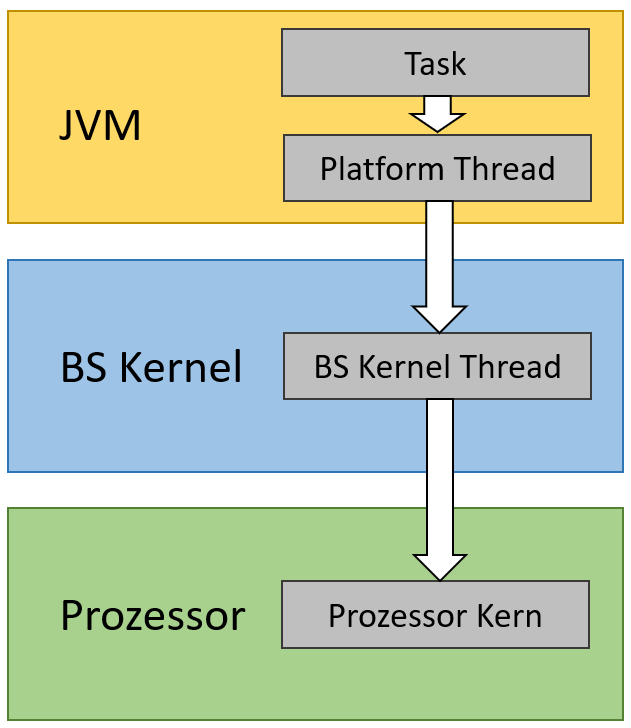
\includegraphics[scale=0.5]{figures/PlatformThreads.png}
	\caption{Aufbau: Java Platform Threads}
	\label{fig:PlatformThreads}
\end{figure}

Dieser Aufbau hat zur Folge, dass Platform Threads schwergewichtig sind. Schwergewichtig meint in diesem Fall, dass ein Platform Thread viel Speicher verbraucht($\sim$ 2-3 MB) und es lange dauert ihn zu erstellen($\sim$ 1ms). Platform Threads und die dazugehörigen Betriebssystem Threads sind also ressourcenintensiv und ihre maximale Anzahl ist somit für ein ausführendes System begrenzt. Dies führt dazu, dass die maximale Anzahl der Platform Threads, weit vor anderen Ressourcen, zum limitierenden Faktor wird. 

Eine Lösung, um zumindest die Kosten für das Erstellen von neuen Platform Threads zu senken, ist das Verwenden von Thread Pools. Hierbei wird eine Gruppe von Aufgaben einem Pool von Platform Threads zugewiesen. In der Regel übersteigt dabei die Anzahl der Aufgaben die Anzahl an Platform Threads. Dies hat zur Folge, dass einem Platform Thread, nachdem er die ihm zugewiesene Aufgabe abgearbeitet hat, direkt eine neue Aufgabe zugewiesen bekommt. Das hat den Vorteil, dass nicht mehr für jede Aufgabe ein neuer Platform Thread erstellt werden muss. Stattdessen können die gleichen Platform Threads wiederverwendet werden um mehrere Aufgaben hintereinander auszuführen. Damit lassen sich zwar die Kosten für das Erstellen von neuen Platform Threads senken, es lässt sich jedoch nicht die maximale Anzahl an Platform Threads erhöhen.

Ein weiteres Problem ist, dass die Verwaltung der Threads vom Betriebssystem über\-nommen wird und die JRE (Java Runtime Environment) keinen Einfluss darauf nehmen kann. Die Verwaltung der Threads auf Betriebssystemebene muss jedoch sehr allgemein gehalten werden, da sie nicht nur für Java, sondern für alle Programmiersprachen funktionieren muss.

\section{Java: Virtual Threads}

Seit dem JDK 21, welches im September 2023 veröffentlicht wurde, sind Virtual Threads ein fester Bestandteil von Java. Sie wurden ursprünglich im Rahmen des Project Loom \cite{loom2024} als sogenannte Fibers entwickelt. Das Ziel war es, die schwergewichtigen Java Threads durch eine leichtgewichtigere Lösung zu ersetzen, welche auf die gleiche API (Application Programming Interface) zurückgreift. Dies soll, Anwendungsentwicklern den Umstieg von Platform Threads auf Virtual Threads erleichtern.

Virtual Threads wurden entwickelt, um die Schwächen von Platform Threads zu adressieren, insbesondere bei Anwendungen, die eine große Zahl von Threads oder häufige Blockierungen aufweisen. Dies gelingt, indem eine große Anzahl Virtual Threads auf eine kleine Zahl Betriebssystem Threads verteilt wird. Dadurch werden die Nachteile von Platform Threads umgangen, dass ihre Anzahl stark begrenzt ist und die Verwaltung der Threads auf Betriebssystemebene stattfindet. Stattdessen können Virtual Threads in großer Zahl erstellt werden und die Verwaltung der Threads findet in der JRE statt.

Im Detail sieht dies wie folgt aus:

Es wird eine kleine Anzahl an Platform Threads(Wrapper) erstellt, die ihrerseits einen Betriebssystem Thread umschließen. Diese Platform Threads werden als Carrier Threads bezeichnet, da sie sozusagen den Virtual Thread tragen. Die Anzahl der Carrier Threads entspricht standardmäßig der Anzahl der Prozessorkerne des ausführenden Systems, kann jedoch je nach Anwendungsfall leicht variieren. Die Carrier Threads werden von einem Fork-Join-Pool verwaltet, der nach dem FIFO-Prinzip (First In - First Out) und mit work-stealing arbeitet.\cite{Pressler2023a}

Für jede neue Aufgabe (task) im System, die nebenläufig ausgeführt werden kann, wird ein neuer Virtual Thread erstellt. Die Aufgabe bleibt dabei die ganze Zeit im gleichen Virtual Thread. Der Virtual Thread wiederum wird zum Bearbeiten der Aufgabe in einen Carrier Thread eingesetzt (mount). 

\begin{figure}[h]
	\centering
	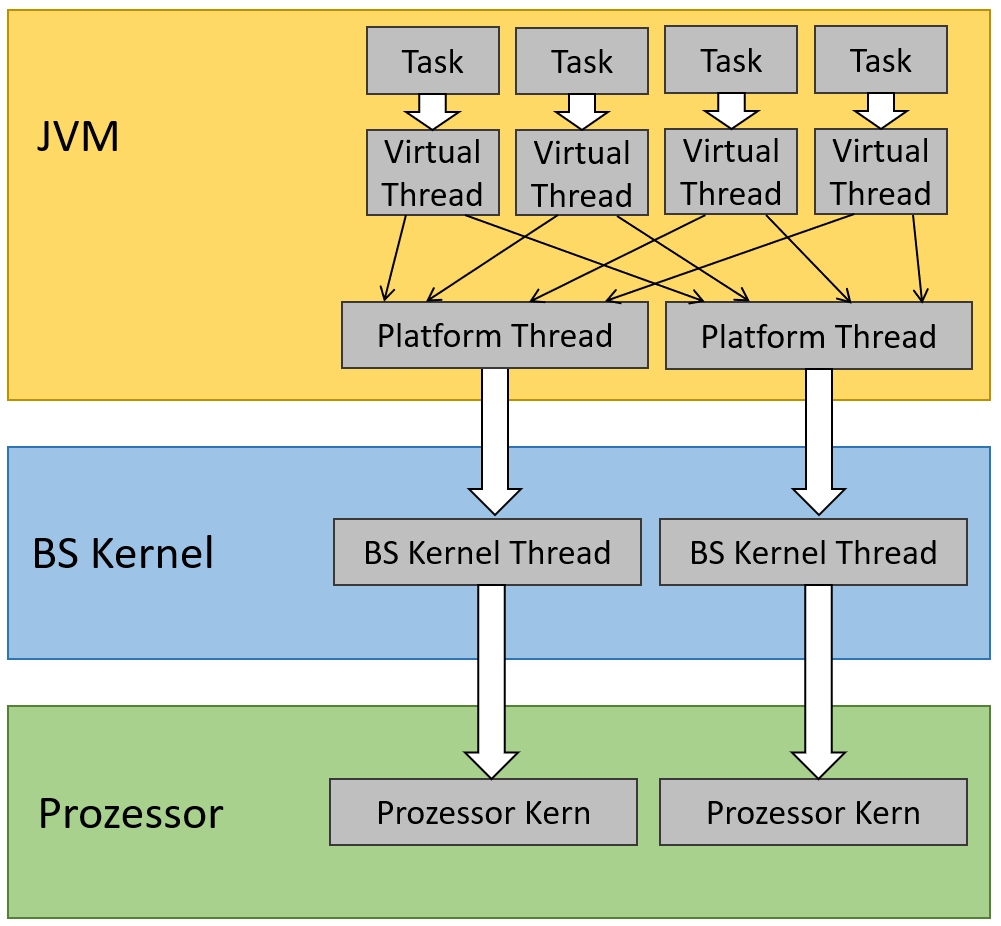
\includegraphics[scale=0.5]{figures/VirtualThreads.png}
	\caption{Aufbau: Java Virtual Threads}
	\label{fig:VirtualThreads}
\end{figure}

Dort bleibt der Virtual Thread so lange, bis die Aufgabe abgeschlossen ist oder der Thread blockiert. Sollte es zu einer Blockade, zum Beispiel durch eine I/O-Operation, kommen, wird der Virtual Thread aus dem Carrier Thread entnommen (unmount) und so lange geparkt, bis er nicht mehr blockiert ist und die Bearbeitung der Aufgabe fortgesetzt werden kann. Der Virtual Thread wird dann wieder in einen freien Carrier Thread eingesetzt, dies kann aber ein anderer sein als zu Beginn. Daraus folgt, eine Aufgabe wird ihre gesamte Lebenszeit vom gleichen Virtual Thread ausgeführt, welcher jedoch in unterschiedliche Carrier Threads eingesetzt werden kann. 

Dies stellt eine entschiedene Neuerung gegenüber den Platform Threads dar. War es bisher so, dass ein Platform Thread fest mit einem Betriebssystem Thread verknüpft war, wurde diese Verknüpfung für Virtual Threads aufgehoben. Dies hat den Vorteil, dass ein Virtual Thread einen Carrier Thread und den damit verbundenen Betriebssystems Thread nur dann benutzt, wenn der Virtual Thread Berechnungen auf dem Prozessor ausführt. Ist ein Virtual Thread blockiert macht er Platz auf dem Betriebssystem Thread für einen anderen Virtual Thread. Bei Platform Threads hingegen blockiert nicht nur der Platform Thread, sondern auch der zugrunde liegende Betriebssystem Thread. \cite{Bateman2023}

\begin{figure}[h]
	\centering
	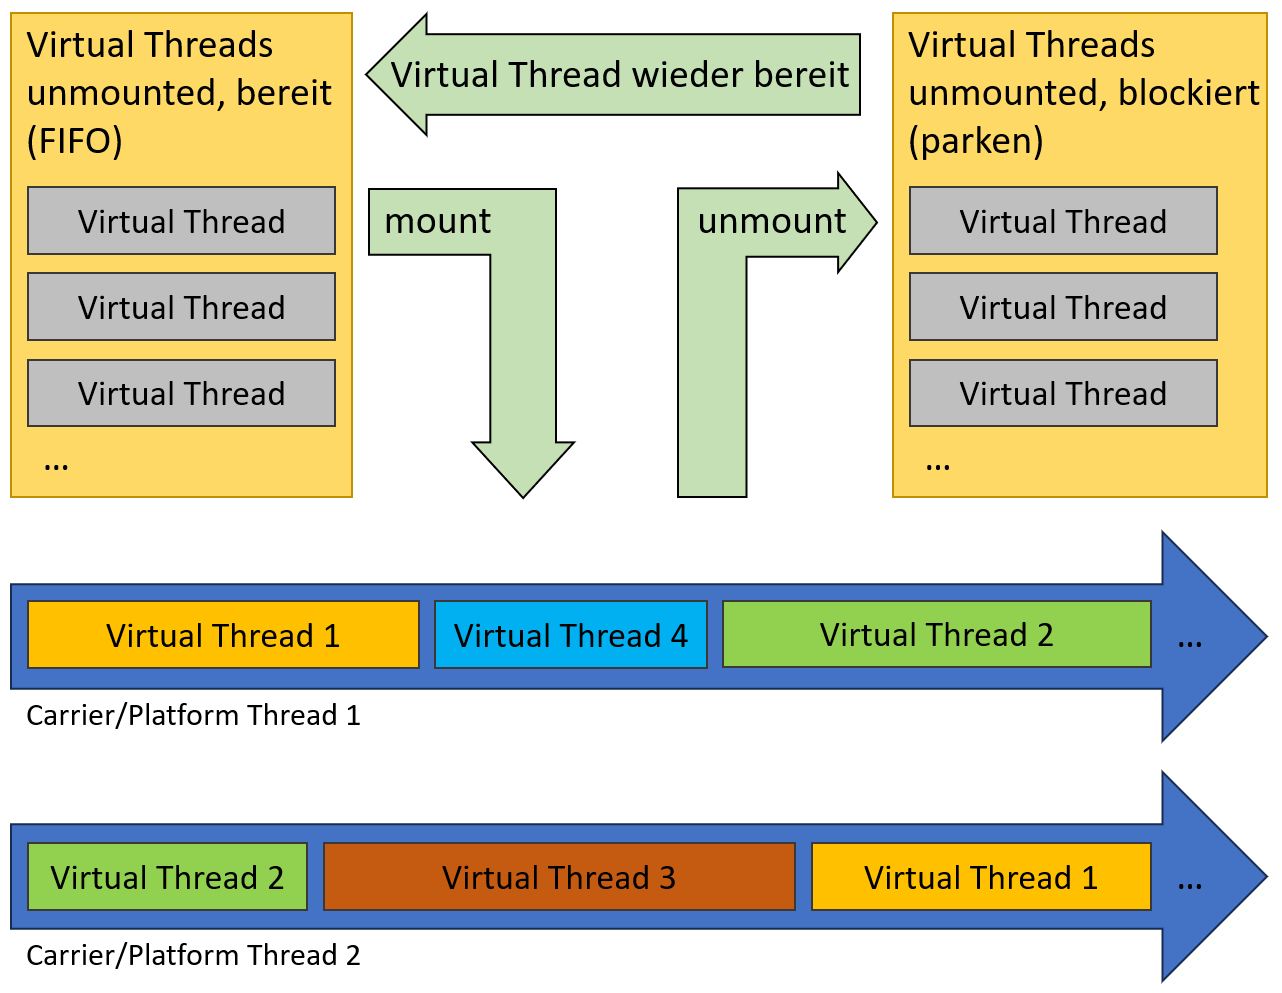
\includegraphics[scale=0.5]{figures/VirtualThreadsAblauf.png}
	\caption{Verwaltung: Java Virtual Threads}
	\label{fig:VirtualThreadsAblauf}
\end{figure}

\subsection{Continuations}

Das beschriebene Starten (mount) und Parken (unmount) von Virtual Threads wird mit Continuations gelöst. Ein Virtual Thread umschließt die ihm übergeben Aufgabe mit einer Continuation. Diese bietet die Methode \code{Continuation.run()} an, um die enthaltene Aufgabe entweder zum ersten Mal zu starten oder sie nach dem Parken fortzusetzen. Letzteres wird auf der Ebene der Continuations als Auftauen (thaw) bezeichnet. Des weiteren gibt es die Methode \code{Continuation.yield()} um eine Aufgabe zu pausieren, wenn sie blockiert. Dies wird im Kontext der Continuations als einfrieren (freeze) bezeichnet. Zuletzt stellen Continuations noch die Methode \code{Continuation.isDone()}(Rückgabewert: boolean) zur Verfügung um zu überprüfen, ob die enthaltene Aufgabe abgeschlossen wurde. Um die Funktionalität der Continuations umzusetzen, musste das gesamte JDK auf Stellen überprüft werden, an denen eine Aufgabe potenziell blockieren kann. An entsprechenden Stellen wurde neuer Code hinzugefügt, der mit den Continuations kommuniziert, um so eine Aufgabe entweder einzufrieren oder später wieder aufzutauen.\cite{Pressler2023b}

Wenn es um das Blockadeverhalten von Virtual Threads, geht gibt es einen Spezialfall, der nach Möglichkeit vermieden werden sollte, das sogenannte Feststecken (pinning). Dies beschreibt den Fall, wenn die im Virtual Thread enthaltene Aufgabe blockiert und der Virtual Thread nicht aus dem ausführenden Carrier Thread entnommen werden kann. Dies führt dazu, dass nicht nur der Virtual Thread, sondern auch der Carrier Thread blockiert. Dies kann entweder dadurch ausgelöst werden, dass der Thread blockiert während er nativen Code aufruft oder der Thread blockiert, während er Code ausführt der sich in einem Synchronized Block befindet. Synchronized wird verwendet, um den gleichzeitigen Zugriff auf eine Methode oder einen Codeblock zu verhindern, damit nur ein Thread zu einem bestimmten Zeitpunkt Zugriff auf den synchronisierten Code hat. Sollte der Code im Synchronized Block lange blockieren kann es sinnvoll sein, das Synchronized durch ein Reentrant Lock zu ersetzen und dieses freizugeben und dann den Platform-Thread abzugeben (unmount). Die Beschränkung durch Synchronized, soll laut den Virtual Thread Entwicklern in einer zukünftigen Version aufgehoben werden\cite{Chilano2024}. Die Beschränkung durch das Aufrufen von nativem Code wird jedoch bestehen bleiben.\cite{Bateman2024}

\subsection{Thread per request Modell}

Ein typischer Anwendungsfall für Virtual Threads ist eine Server-Anwendung, die Anfragen im Thread per request Modell bearbeitet. Für jede neue Anfrage wird ein neuer Thread erstellt, der diese Anfrage bearbeitet. So können mehrere Anfragen nebenläufig bearbeitet werden. Dies würde bei Platform Threads bedeuten, dass für jede neue Anfrage nicht nur ein neuer Platform Thread, sondern auch ein neuer Betriebssystem Threads erstellt werden muss. Da aber die Anzahl an Betriebssystem Threads für ein System stark limitiert ist, in der Regel auf einige Tausend, ist damit auch die Anzahl der nebenläufig zu bearbeitenden Anfragen limitiert. So werden Platform Threads zum limitierenden Faktor des Systems. Virtual Threads hingegen sind deutlich leichtgewichtiger, da ihre Anzahl nicht an die zur Verfügung stehenden Betriebssystem Threads gebunden ist. Dadurch lässt sich eine große Anzahl von ihnen erstellen, bis zu mehrere Millionen.

Der Vorteil von Virtual Threads gegenüber Platform Threads bei dem Thread per request Modell, lässt sich gut an Little's Gesetz \cite{Little1961} zeigen. Es besagt, dass die sich gleichzeitig in Bearbeitung befindlichen Aufgaben(L) davon abhängig sind, wie hoch der Durchsatz($\lambda$) und die Durchlaufzeit (W) sind.

\begin{eqnarray}
	L = \lambda \cdot W \nonumber
\end{eqnarray}

Auf das Thread per request Modell angewandt bedeutet das, dass der Durchsatz die pro Sekunde in das System eingehenden Anfragen ist. Die Durchlaufzeit wird dadurch beschrieben, wie hoch die durchschnittliche Latenz des Systems ist, um eine Anfrage zu beantworten. L ist weiterhin die sich gleichzeitig in Bearbeitung befindlichen Aufgaben.

\begin{align*}
	\text{gleichzeitig in Bearbeitung befindliche Aufgaben} &= 
	\text{Anfragen pro Sekunde} \cdot \text{Latenz}
\end{align*}

Gehen wir also von einem System aus, das 200 Anfragen pro Sekunde verarbeitet, bei einer Latenz von 50ms pro Anfrage. Dafür ist es nötig 10 Anfragen gleichzeitig nebenläufig zu verarbeiten. Soll das System nun auf 2000 Anfragen pro Sekunde, bei gleichbleibender Latenz, skaliert werden, muss das System nun 100  Anfragen gleichzeitig nebenläufig verarbeiten \cite{Pressler2023a}.

Da wir vom Thread per request Modell ausgehen, müssen also im Fall von  Platform Threads 100 von ihnen erstellt werden und damit auch 100 Betriebssystem Threads. Somit ist die Skalierbarkeit auf die maximal zur Verfühgung stehenden Betriebssystem Threads (einige Tausend) begrenzt. Virtual Threads hingegen lassen sich in einer deutlich größeren Anzahl erstellen (mehrere Millionen) und werden so nicht zum limitierenden Faktor wenn es um die Skalierbarkeit des beschriebenen Beispiels geht.

Diese Annahme stimmt allerdings nur so lange, wie die nebenläufig bearbeiteten Aufgaben weiterhin mit der gleichen Latenz bearbeitet werden. Dies ist zum Beispiel dann der Fall, wenn eine Aufgabe pausiert wird, um auf eine I/O-Operation zu warten. Wenn die einzelne Aufgaben jedoch rechenintensiv sind und möglicherweise niemals pausieren, verlieren Virtual Threads ihren Vorteil gegenüber Platform Threads. Virtual Threads können nicht einzelne Aufgaben schneller ausführen als Platform Threads, sondern mehr Aufgaben nebenläufig bearbeiten, falls die Aufgaben manchmal blockieren. 

Damit lässt sich abschließend sagen, dass Virtual Threads den Durchsatz einer Anwendung gegenüber Platform Threads steigern, wenn viele Aufgaben nebenläufig ausgeführt werden und diese Aufgaben manchmal pausieren müssen.

\subsection{Softwareentwicklung mit Virtual Threads}

Eine weitere Zielsetzung von Virtual Threads war es, Softwareentwicklern den Umstieg von Plattform Threads zu Virtual Threads so einfach wie möglich zu gestalten. Deshalb sind Virtual Threads genau wie Plattform Threads eine Instanz der \code{java.lang.Thread} API. So ist es relativ einfach möglich Virtual Threads zu integrieren, ohne die bestehende Codebasis wesentlich zu verändern.

Am folgendem Code-Beispiel wird deutlich, dass lediglich der Aufruf \code{new Thread())} durch \code{Thread.ofVirtual().start()} ersetzt werden muss. Das Starten des Virtual Threads passiert jetzt direkt beim Aufruf. Der restliche Code bleibt jedoch unberührt.

\begin{lstlisting}[language=Java]
	// erstellen eines einzelnen Platform Threads	
	Thread platformThread = new Thread(() -> System.out.println("Platform Thread"));
	platformThread.start();
	platformThread.join();

	// erstellen eines einzelnen Virtual Threads
	Thread virtualThread = Thread.ofVirtual().start(() -> System.out.println("Virtual Thread"));
	virtualThread.join();
\end{lstlisting}

Für Virtual Threads wurde der neue Executor Service \code{Executors.""new""Virtual""Thread""Per""Task""Executor()} entwickelt. Für jeden Aufruf von \texttt{ExecutorService.""submit(""Run""nable)} wird ein neuer Virtual Thread erstellt, der die ihm zugewiesene Aufgabe ausführt. Der Rückgabewert des Executor Service ist ein Future, welches das Ergebnis der Aufgabe enthält, sobald der erstellte Virtual Thread ausgeführt wurde. Mit Hilfe von \code{Executors.""new""Virtual""Thread""Per""Task""Executor()} lässt sich ein bestehender Code leicht von Platform Threads auf Virtual Threads umstellen. Oft wird für das Verwalten von Platform Threads ein Thread Pool erstellt und für das Erstellen eines Thread Pools ein Executor Service verwendet. So könnten die Plattform Threads beispielsweise bisher in \code{Executors.newCachedThreadPool()} verwaltet worden sein. Dieser lässt sich nun leicht durch \code{Executors.new""Virtual""Thread""Per""Task""Executor()} ersetzen. Dies wird auch am folgenden Beispiel deutlich:

\begin{lstlisting}[language=Java]
	// mehrere Platform Threads mit Executors.newCachedThreadPool() erstellen
	try (var cachedPool = Executors.newCachedThreadPool()) {
		var future1 = cachedPool.submit(() -> powerFunction(task1.base, task1.exponent));
		var future2 = cachedPool.submit(() -> powerFunction(task2.base, task2.exponent));
		int ptResult1 = future1.get();
		int ptResult2 = future2.get();
		System.out.println("Platform Thread Result 1: " + ptResult1);
		System.out.println("Platform Thread Result 2: " + ptResult2);
	} catch (ExecutionException | InterruptedException e) {
		throw new RuntimeException(e);
	}
	// mehrere Virtual Threads mit Executors.newVirtualThreadPerTaskExecutor() erstellen
	try (var executor = Executors.newVirtualThreadPerTaskExecutor()) {
		var future1 = executor.submit(() -> powerFunction(task1.base, task1.exponent));
		var future2 = executor.submit(() -> powerFunction(task2.base, task2.exponent));
		int vtResult1 = future1.get();
		int vtResult2 = future2.get();
		System.out.println("Virtual Thread Result 1: " + vtResult1);
		System.out.println("Virtual Thread Result 2: " + vtResult2);
	} catch (ExecutionException | InterruptedException e) {
		throw new RuntimeException(e);
	}
\end{lstlisting}
Der \code{Executors"".new""Virtual""Thread""Per""Task""Executor()} erstellt für jede Aufgabe einen neuen Virtual Thread und dient nicht als klassischer Thread Pool, wie der \code{Executors.""new""Cached""Thread""Pool()}. Stattdessen wird jede Aufgabe direkt in einem neuen Virtual Thread ausgeführt. Virtual Threads benötigen keinen von der Anwendung explizit verwalteten Thread Pool, da sie von der JVM automatisch auf Plattform-Threads ausgeführt werden. Diese Plattform-Threads werden intern in einem eigenen Thread Pool verwaltet. Der \code{Executors.new""Virtual""Thread""Per""Task""Executor()} nutzt lediglich die gleiche API wie der \code{Executors.new""Cached""ThreadPool()} um den Wechsel von Platform Threads auf Virtual Threads so unkompliziert wie möglich zu gestalten.

Die maximale Anzahl von Virtual Threads ist deutlich größer als die von Platform Threads und die Zeit sie zu erstellen sowie ihr Speicherverbrauch sind deutlich geringer. Bei der Umstellung auf Virtual Threads werden Platform Threads also nicht direkt durch Virtual Threads ersetzt. Stattdessen werden die Aufgaben durch Virtual Threads ersetzt, beziehungsweise für jede Aufgabe wird ein neuer Virtual Thread erstellt. 

Falls ein Thread Pool bei Platform Threads bisher verwendet wurde um die Anzahl an maximal nebenläufig ausgeführten Aufgaben zu limitieren, sollte dafür bei Virtual Threads stattdessen auf Semaphore zurückgegriffen werden. Auch mit Semaphoren lässt sich die maximale Anzahl gleichzeitiger Zugriffe auf eine Ressource limitieren.

\subsection{Zusammenfassung: Java Virtual Threads}

Virtual Threads stellen eine bedeutende Weiterentwicklung in der Nebenläufigkeits\-mo\-del\-lie\-rung in Java dar. Durch die Entkopplung von Virtual Threads und Betriebssystem-Threads wird ein hoher Grad an Parallelisierung ermöglicht, ohne die Einschränkungen der herkömmlichen Thread-Pools, in denen für jeden Platform Thread ein Betriebssystem-Thread erstellt wird.

Ein weiterer Vorteil ist die verbesserte Thread-Verwaltung: Die Verwaltung der Threads findet in der Java Runtime Environment (JRE) statt, was eine optimierte und anwendungsspezifische Steuerung ermöglicht. Dies erlaubt der JRE, Virtual Threads effizient auf Carrier Threads zu verteilen, wodurch eine bessere Ressourcennutzung erreicht wird.

In typischen Anwendungsfällen wie dem Thread-per-Request-Modell zeigen Virtual Threads ihre Stärke, indem sie die Skalierbarkeit erheblich erhöhen, da Millionen von Threads effizient verwaltet werden können. Allerdings bleibt ihr Nutzen auf Szenarien beschränkt, in denen Aufgaben regelmäßig blockieren und somit Platz für andere Threads auf den Carrier Threads schaffen. In CPU-intensiven Szenarien, bei denen keine Pausierung stattfindet, können Virtual Threads keinen signifikanten Vorteil gegenüber Platform Threads bieten.

Die Kompatibilität mit bestehenden Thread-API macht eine einfache Migration von Platform Threads zu Virtual Threads möglich. Dennoch existieren Einschränkungen, wie das Risiko des „Pinnings“ bei nativen oder synchronisierten Codeabschnitten, die bei der Verwendung von Virtual Threads berücksichtigt werden müssen.

Insgesamt sind Virtual Threads ein leistungsstarkes Werkzeug für Entwickler, um Anwendungen mit hoher Nebenläufigkeit effizient zu implementieren, solange deren spezifische Einschränkungen beachtet werden.

\newpage

\section{Kotlin: Coroutinen}

Coroutinen sind ein zentrales Konzept in Kotlin und werden für die asynchrone Programmierung sowie für nebenläufige Prozesse genutzt. Sie ermöglichen es, komplexe Abläufe einfacher zu schreiben und verständlicher zu gestalten. Im Gegensatz zu herkömmlichen Threads sind Coroutinen jedoch leichtgewichtiger und blockieren keinen Thread während ihrer Ausführung. Dies wird durch die Nutzung eines Thread-Pools ermöglicht, auf dem Coroutinen kooperativ ausgeführt werden. Dieses Kapitel wird die Grundlagen von Coroutinen, deren Implementierung und fortgeschrittene Anwendungsfälle erklären.

\subsection{Motivation}

Bevor es Coroutinen in Kotlin gab, wurde asynchroner Code häufig mit Callbacks umgesetzt. Dabei handelt es sich um ein Programmierkonzept, bei dem einer Funktion als Argument eine andere Funktion übergeben wird, um zu einem späteren Zeitpunkt aufgerufen zu werden. Dies ermöglicht eine flexible und modulare Strukturierung von Programmen, da verschiedene Operationen oder Ereignisse mit spezifischen Reaktionen verknüpft werden können. 

In der Programmierung unterscheidet man zwischen synchroner und asynchroner Aus\-füh\-rung:

Synchrone Ausführung bedeutet, dass der Code in der Reihenfolge ausgeführt wird, in der er geschrieben steht. Das heißt, die Ausführung einer Funktion blockiert den weiteren Ablauf des Programms, bis sie abgeschlossen ist. Ein Beispiel für synchrone Ausführung wäre, wenn wir auf das Ergebnis einer Dateioperation warten und das Programm erst dann fortsetzt wird, wenn das Ergebnis vorliegt.

Asynchrone Ausführung bedeutet, dass eine Funktion gestartet wird, aber das Programm nicht darauf wartet, dass sie abgeschlossen wird. Stattdessen kann das Programm während der Ausführung dieser Funktion andere Aufgaben fortsetzen, ohne blockiert zu werden. Bei asynchroner Ausführung können Callbacks genutzt werden, um das Ergebnis der Funktion zu verarbeiten, wenn sie abgeschlossen ist.

Callbacks sind besonders nützlich in der asynchronen Programmierung, da Operationen wie das Lesen von Dateien, das Abrufen von Daten über das Netzwerk oder das Warten auf Benutzereingaben ohne Blockieren des Hauptprogramms ausgeführt werden können.

Das folgende Beispiel zeigt, wie asynchrone Operationen mithilfe von Callbacks umgesetzt werden:

\begin{lstlisting}[language=Kotlin]
	import java.io.File
	import kotlin.concurrent.thread
	
	fun readFileAsync(filename: String, callback: (String) -> Unit) {
		thread {
			val content = File(filename).readText()
			callback(content)
		}
	}
	
	fun main() {
		readFileAsync("example.txt") { content ->
			println("File Content: $content")
		}
		println("Read File...")
	}
\end{lstlisting}

In dem gezeigten Beispiel liest die Funktion \texttt{readFileAsync} den Inhalt einer Datei in einem separaten Thread ein und verwendet einen Callback, um das Ergebnis zu verarbeiten. Der Callback wird als Lambda-Ausdruck an \texttt{readFileAsync} übergeben und ausgeführt, nachdem das Einlesen abgeschlossen ist. Der Haupt-Thread wird währenddessen nicht blockiert und kann andere Aufgaben ausführen.

Da es sich bei dem gezeigten Beispiel um eine asynchrone Ausführung handelt kann nicht vorhergesehen werden ob erst \texttt{"File Content: [Dateiinhalt]"} oder \texttt{"Read File..."} ausgegeben wird, da die Dateioperation auf einem separaten Thread ausgeführt wird.

Würde das Starten des Threads in \texttt{readFileAsync} weggelassen, würde es sich um einen synchronen Aufruf handeln. Die Ausgabe wäre dann zuerst \texttt{"File Content: ""[Datei""inhalt]"} und danach \texttt{"Read File..."}, da der Haupt-Thread auf das Ergebnis der Dateioperation warten würde, bevor er fortfährt.

Callbacks sind folglich eine gängige Variante um asynchronen Code zu schreiben. Ein Nachteil jedoch ist die Verwendung vieler verschachtelter Callbacks, welche umgangssprachlich als Callback Hell bezeichnet werden\cite{Leger2021}. Die Callback Hell führt dazu, dass der Code schwer lesbar wird. Daraus resultiert eine erhöhte Komplexität bei der Wartung und dem Debuggen. Die Verschachtelungen machen die Rückverfolgung des Programmflusses kompliziert und  die Fehlerbehandlung wird immer aufwendiger, da sie auf jeder Ebene der Verschachtelungen stattfinden muss.

\begin{lstlisting}[language=Kotlin]
	import kotlin.concurrent.thread
	import kotlin.Result

	// Simuliert eine asynchrone, zeitaufwändige I/O-Operation (z.B. Datei lesen)
	fun readFileAsync(callback: (Result<String>) -> Unit) {
		thread {
			try {
				Thread.sleep(500)
				callback(Result.success("File Content"))
			} catch (e: Exception) {
				callback(Result.failure(e))
			}
		}
	}

	// Simuliert eine asynchrone, zeitaufwändige Netzwerkoperation, bei der Daten verarbeitet werden (z.B. API-Anfrage)
	fun processData(input: String, callback: (Result<String>) -> Unit) {
		thread {
			try {
				Thread.sleep(500)
				callback(Result.success("$input -> Processed Data"))
			} catch (e: Exception) {
				callback(Result.failure(e))
			}
		}
	}

	// Simuliert das asynchrone, zeitaufwändige Speichern von Daten (z.B. in einer Datenbank oder Datei)
	fun saveData(input: String, callback: (Result<String>) -> Unit) {
		thread {
			try {
				Thread.sleep(500)
				callback(Result.success("$input -> Data Saved"))
			} catch (e: Exception) {
				callback(Result.failure(e))
			}
		}
	}

	fun main() {
		// Callbacks werden verwendet, um das Ergebnis schrittweise zu erhalten
		readFileAsync { result1 ->
			result1.onSuccess { res1 ->
				processData(res1) { result2 ->
					result2.onSuccess { res2 ->
						saveData(res2) { result3 ->
							result3.onSuccess { res3 ->
								println("Final Result: $res3") // Ausgabe des finalen Ergebnisses
							}
							// Fehlerbehandlung für saveData
							result3.onFailure { error ->
								println("Error in saveData: ${error.message}")
							}
						}
					}
					// Fehlerbehandlung für processData
					result2.onFailure { error ->
						println("Error in processData: ${error.message}")
					}
				}
			}
			// Fehlerbehandlung für readFileAsync
			result1.onFailure { error ->
				println("Error in readFileAsync: ${error.message}")
			}
		}
		// Zeigt an, dass die asynchronen 	Operationen gestartet wurden
		println("Started operations...")
	}
\end{lstlisting}
Konsolenausgabe:
\begin{lstlisting}[frame=shadowbox, rulecolor=\color{black}, backgroundcolor=\color{gray!10}]
	Started operations...
	Final Result: File Content -> Processed Data -> Data Saved
\end{lstlisting}

In diesem Beispiel werden drei Operationen asynchron mit Callbacks ausgeführt, die jeweils das Ergebnis der vorausgehenden Operation benötigen. Dies führt zu einer Verschachtelung der Aufrufe in der Main-Funktion. Selbst in diesem einfachen Bespiel wird der Code schon deutlich schwerer lesbar im Vergleich zu einer synchronen Programmierweise, nicht zuletzt auf Grund der ebenfalls verschachtelten Fehlerbehandlung.

Genau an diesem Punkt setzt die Entwicklung von Coroutinen an, welche als Ziel haben die Nachteile der Callback Hell zu umgehen und dabei trotzdem die Vorteile der Callbacks zu behalten\cite{Elizarov2017a}. Ermöglicht werden soll das nebenläufige Ausführen von Aufgaben, ohne das Hauptprogramm zu blockieren, bei weiterhin gut lesbarem Code.


\subsection{suspend-Modifier}
\label{subsec:suspend}

Um die Nachteile der Callback-Hell zu umgehen, verfolgen die Coroutinen den Ansatz, synchronen Code zu schreiben, der anschließend asynchron ausgeführt wird. Dafür wurde das Schlüsselwort \texttt{suspend} eingeführt\cite{Akhin2024}. Es wird verwendet um Funktionen als suspendierbar (oder "pausierbar") zu kennzeichnen. Es ermöglicht einer Funktion, ihre Ausführung zu unterbrechen und später fortzusetzen, ohne dabei den aktuellen Thread zu blockieren (wird im Detail in Abschnitt \ref{subsec:csp} erläutert). Dies ist besonders nützlich für die asynchrone Programmierung, da es den Code im Vergleich zu traditionellen Callback- oder Thread-basierten Lösungen lesbarer und einfacher zu handhaben macht. Außerdem werden mit \texttt{async} Coroutinen gestartet, welche die \texttt{suspend}-Funktionen ausführen. Dadurch kann das Code-Beisipiel aus dem vorausgehenden Abschnitt folgendermaßen optimiert werden:

\begin{lstlisting}[language=Kotlin]
	import kotlinx.coroutines.*

	// Simuliert eine asynchrone, zeitaufwändige I/O-Operation (z.B. Datei lesen)
	suspend fun readFileAsync(): String {
		delay(500)
		return "File Content"
	}

	// Simuliert eine asynchrone, zeitaufwändige Netzwerkoperation, bei der Daten verarbeitet werden (z.B. API-Anfrage)
	suspend fun processData(input: String): String {
		delay(500)
		return "$input -> Processed Data"
	}

	// Simuliert das asynchrone, zeitaufwändige Speichern von Daten (z.B. in einer Datenbank oder Datei)
	suspend fun saveData(input: String): String {
		delay(500)
		return "$input -> Data Saved"
	}

	fun main() = runBlocking {
		try {
			// Startet alle Operationen gleichzeitig mit 'async' und wartet auf deren Ergebnisse
			val deferred1 = 
				async { readFileAsync() }
			val deferred2 = 
				async { processData(deferred1.await()) }
			val deferred3 = 
				async { saveData(deferred2.await()) }
		
			// Warten auf die Ergebnisse und Ausgabe des finalen Ergebnisses
			println("Final Result: ${deferred3.await()}")
		} catch (e: Exception) {
			println("Error: ${e.message}")
		}
		// Zeigt an, dass die asynchronen Operationen gestartet wurden
		println("Started operations...")  
	}
\end{lstlisting}
Konsolenausgabe:
\begin{lstlisting}[frame=shadowbox, rulecolor=\color{black}, backgroundcolor=\color{gray!10}]
	Started operations...
	Final Result: File Content -> Processed Data -> Data Saved
\end{lstlisting}

In dem Beispiel werden jene Funktionen mit dem \texttt{suspend}-Schlüsselwort gekennzeichnet, die als asynchrone Operationen ausgeführt werden sollen. Generell ist bei der Verwendung von \texttt{suspend}-Funktionen zu beachten, dass sie nur von anderen \texttt{suspend}-Funktionen oder Coroutinen ausgeführt werden können. Deshalb werden mit \texttt{async} insgesamt drei Coroutinen gestartet welche die {suspend}-Funktionen asynchron ausführen. Wie genau Coroutinen gestartet werden wird im nächsten Abschnitt gezeigt.

Durch das Verwenden des suspend-Modifiers ist es möglich, in der Main-Funktion eine synchrone Schreibweise zu verwenden, obwohl der Code asynchron ausgeführt wird ohne Threads zu blockieren. Dadurch haben Coroutinen zwei entscheidende Vorteile gegenüber Callbacks. Ersten ist der Code deutlich besser lesbar, da es weder bei den Funktionsaufrufen noch bei der Fehlerbehandlung zu Verschachtelungen kommt und zweitens blockieren keine Threads bei der asynchronen Ausführung der \texttt{suspend}-Funktionen. Damit stellen Coroutinen einen deutlichen Fortschritt gegenüber Callbacks dar. 

\subsection{Coroutinen starten}
\label{subsec:corostarten}

Um in Kotlin eine Coroutine zu starten wird ein Coroutinen-Builder verwendet. Nachfolgend werden  die am häufigsten verwendeten Coroutinen-Builder aufgeführt:

\begin{itemize}
	\item \textbf{launch} ist der am häufigsten verwendete Coroutinen-Builder und startet eine neue Coroutine, die kein Ergebnis zurückgibt. Er wird hauptsächlich für asynchron auszuführende Aufgaben verwendet, die nach dem fire-and-forget Prinzip gestartet werden.
	\item \textbf{async} startet ebenfalls eine neue Coroutine, gibt aber ein Deferred-Objekt zurück, das ein zukünftiges Ergebnis repräsentiert. Bei Deferred handelt sich um das Äquivalent eines Promise oder Future in Kotlin. Mit \texttt{await()} ist es möglich, auf das Ergebnis zu warten.
	\item \textbf{runBlocking} blockiert den aktuellen Thread, bis der Coroutine-Block abgeschlossen ist. Dies ermöglicht es, asynchronen Code in einer synchronen Umgebung auszuführen. Er wird hauptsächlich in Main-Funktionen und Testfällen verwendet.
	\item \textbf{produce} ist ein spezieller Coroutine-Builder, der einen \texttt{ReceiveChannel} erstellt und Werte in diesen Kanal sendet. Der Kanal wird automatisch geschlossen, wenn die Coroutine beendet wird oder eine Ausnahme auftritt. Der Builder wird haupt\-säch\-lich für Producer-Consumer-Muster verwendet.
\end{itemize}


\subsubsection{Coroutinen-Builder}

Das folgende Beispiel zeigt den Aufbau eines Coroutinen-Builders anhand der Funktionssignatur des Builders \texttt{launch}.

\begin{lstlisting}[language=Kotlin]
	fun CoroutineScope.launch(
		context: CoroutineContext = EmptyCoroutineContext,
		start: CoroutineStart = CoroutineStart.DEFAULT,
		block: suspend CoroutineScope.() -> Unit
	): Job
\end{lstlisting}

Die Funktionssignatur besteht aus dem Empfänger-Typ \texttt{CoroutineScope}, dem Funktionsnamen \texttt{launch}, den Parametern \texttt{context}, \texttt{start}, \texttt{block} und dem Rückgabewert \texttt{Job}.

Der Empfänger-Typ \texttt{CoroutineScope} gibt an, in welchem Scope die Coroutine ausgeführt wird. Builder werden als Erweiterungsfunktionen von Scopes ausgeführt und starten die Coroutine in dem entsprechenden Scope. Durch Scopes lassen sich große Mengen von Coroutinen strukturieren. Dies wird im Kapitel \ref{subsec:coroutinescope} genauer erörtert.

Der Parameter \texttt{context} gibt die Rahmenbedingungen vor, unter denen die Coroutine ausgeführt werden soll. Die einzelnen Bestandteile eines Contextes werden im Kapitel \ref{subsec:coroutinecontext} erklärt.

Der Parameter \texttt{start} gibt an, wann die Coroutine gestartet wird. Dafür kann eine \texttt{Coroutine""Start} Enumeration übergeben werden. Der Standardwert ist \texttt{Coroutine""Start.""DEFAULT}, was bewirkt, dass die Coroutine sofort gestartet wird.

Im Parameter \texttt{block} wird der von der Coroutine auszuführende Code gespeichert. Wie der Code konkret von der Coroutine ausgeführt wird, wird im Kapitel \ref{subsec:csp} genauer erklärt.

Abschließend hat der Builder als Rückgabewert ein Job-Objekt. Seine Funktionsweise wird im nachfolgendem Kapitel beschrieben.


\subsection{Job}

Ein Job-Objekt in Kotlin repräsentiert eine Coroutine und ihreren Lebenszyklus. Ein Job wird verwendet, um den Status einer Coroutine zu überwachen und zu kontrollieren. Der Coroutinen-Builder \texttt{launch} hat zum Beispiel ein Job-Objekt als Rückgabewert für genau diesen Zweck. Um den Status der Coroutine zu überwachen stehen folgende Eigenschaften zur Verfügung:

\begin{itemize}
	\item \textbf{isActive:} Gibt \texttt{true} zurück, wenn der Job aktiv und nicht abgeschlossen oder abgebrochen ist.
	\item \textbf{isCompleted:} Gibt \texttt{true} zurück, wenn der Job abgeschlossen ist.
	\item \textbf{isCancelled:} Gibt \texttt{true} zurück, wenn der Job abgebrochen wurde.
\end{itemize}

Um eine Coroutine zu kontrollieren stellt ein Job folgende Funktionen zur Verfügung:

\begin{itemize}
	\item \textbf{start():} Startet den Job, falls er noch nicht gestartet wurde.
	\item \textbf{cancel():} Bricht den Job ab. Alle untergeordneten Coroutinen werden ebenfalls abgebrochen.
	\item \textbf{join():} Eine suspend-Funktion, die wartet, bis der Job abgeschlossen ist.
	\item \textbf{invokeOnCompletion(handler: CompletionHandler):} Fügt einen Handler hinzu, der ausgeführt wird, wenn der Job abgeschlossen ist.
\end{itemize}

Auch das Deferred-Objekt ist ein Job-Objekt für Coroutinen die ein Ergebnis liefern. Dieses wird beispielsweise von dem \texttt{async} Coroutinen-Builder zurückgeben. Neben den oben genannten Eigenschaften und Methoden bietet es folgende weitere Funktionen, um die Funktionalität eines Futures erfüllen zu können:

\begin{itemize}
	\item \textbf{await():} Eine suspend-Funktion, die auf das Ergebnis der Coroutine wartet und es zurückgibt.
	\item \textbf{getCompleted():} Gibt das Ergebnis zurück, wenn die Coroutine abgeschlossen ist, oder löst eine Ausnahme aus, wenn die Coroutine noch nicht abgeschlossen ist oder mit einem Fehler beendet wurde.
\end{itemize}

\subsection{Dispatcher}

Beim Starten einer Coroutine mittels Coroutinen-Builder kann ein sogenannter Dispatcher für die Coroutine festgelegt werden. Der Dispatcher bestimmt auf welchem Thread oder Thread-Pool die Coroutine ausgeführt wird. In der Regel wird einer der vier folgenden Dispatcher verwendet:

\subsubsection{Dispatchers.Default}

\begin{itemize}
	\item Wird für CPU-intensive Aufgaben verwendet.
	\item Nutzt einen gemeinsamen Pool von Hintergrund-Threads. Die Anzahl der Threads entspricht der Anzahl der CPU-Kerne, mindestens jedoch 2 Threads.
	\item Der Scheduler nutzt eine Work-Stealing-Strategie für eine maximierte CPU-Auslastung.
	\item Ideal für rechenintensive Operationen, die keine sofortige Benutzerinteraktion erfordern.
	\item Ist der Standard Dispatcher in gängigen Buildern wie launch oder asynch.
\end{itemize}


\subsubsection{Dispatchers.IO}

\begin{itemize}
	\item Optimiert für I/O-intensive Aufgaben wie Netzwerk- und Datenbankoperationen oder das Lesen und Schreiben von Dateien.
	\item Nutzt einen Pool von Threads, der für I/O-Operationen konfiguriert ist.  Standardmäßig enthält er 64 Threads, kann aber bei Bedarf erweitert werden.
	\item Der Scheduler nutzt eine FIFO-Warteschlange für die effiziente Bearbeitung von I/O-Operationen.
	\item Hilft, die Haupt-Threads von langwierigen I/O-Operationen zu entlasten.
\end{itemize}

\subsubsection{Dispatchers.Main}

\begin{itemize}
	\item Wird für Aufgaben verwendet, die auf dem Haupt-Thread ausgeführt werden müssen, z.B. UI-Aktualisierungen.
	\item In Android-Anwendungen ist dies der Haupt-Thread, der für die Benutzeroberfläche verantwortlich ist.
\end{itemize}

\subsubsection{Dispatchers.Unconfined}

\begin{itemize}
	\item Führt Coroutinen im aktuellen Thread aus, bis sie suspendiert werden.
	\item Nach der Suspendierung wird die Coroutine in dem Thread fortgesetzt, der die Wiederaufnahme vornimmt.
	\item Ist hauptsächlich für spezielle Anwendungsfälle gedacht, zum Beispiel  Testing.
\end{itemize}

\subsubsection{StandardTestDispatcher}

\begin{itemize}
	\item Speziell für Tests entwickelt, um deterministisches und kontrolliertes Verhalten von Coroutinen zu gewährleisten.
	\item Bietet eine manuelle Kontrolle über die Ausführung von Coroutinen, sodass Testfälle vorhersehbar und präzise gestaltet werden können.
	\item Im Gegensatz zu anderen Dispatchern führt er keine Coroutinen automatisch aus. Stattdessen müssen sie explizit durch den Test gesteuert werden, z.B. durch Methoden wie \texttt{advanceTimeBy} oder \texttt{runCurrent}.
	\item Ersetzt \texttt{Dispatchers.Unconfined} in Tests, um unerwartetes Verhalten durch spontane Thread-Wechsel zu vermeiden.
\end{itemize}

Die Vorteile des Dispatcher-Ansatzes sind dabei leicht ersichtlich. Mit Hilfe der Dispatcher findet eine Abstrahierung der Thread-Verwaltung statt und es wird Komplexität reduziert. Ein Anwender muss nur noch einen Dispatcher wählen, der für die zugewiesene Aufgabe optimiert wurde. Außerdem wird der Code besser lesbar, da sich einem Außenstehenden sofort erschließt, für was für eine Sorte von Aufgabe die Coroutine erstellt wurde. Die Herausforderung für den Anwender ist dabei die Wahl des passenden Dispatchers, da diese für bestimmte Anwendungsfälle optimiert wurden. Außerdem sollte von häufigen Kontextwechseln während der Laufzeit einer Coroutine abgesehen werden, da dies jedes Mal zu einem kleinen  Performance-Overhead führt.

Die Zuweisung eines Dispatchers während des Startens einer Coroutine mit dem Builder \texttt{launch} sieht folgendermaßen aus:

\begin{lstlisting}[language=Kotlin]
	launch(Dispatchers.Default) {
		// CPU-intensive Aufgabe
	}
\end{lstlisting}

\subsection{Coroutinen-Context}
\label{subsec:coroutinecontext}

Das Code-Beispiel aus dem vorangegangenen Kapitel für die Zuweisung eines Dispatchers ist etwas verkürzt, denn ein Coroutinen-Builder benötigt eigentlich einen Coroutinen-Context. Ein Coroutinen-Context wiederum setzt sich aus einem Job, einem Dispatcher und einem Coroutinen-Namen zusammen. Diese Elemente geben die Rahmenbedingungen vor, unter denen eine Coroutine ausgeführt werden soll. Möchte man alle drei Elemente selber festlegen sähe dies wie folgt aus:

\begin{lstlisting}[language=Kotlin]
	import kotlinx.coroutines.*

	fun main() = runBlocking {
		val customContext = Job() + Dispatchers.Default + CoroutineName("MyCoroutine")
	
		launch(customContext) {
			// CPU-intensive Aufgabe
		}
	}
\end{lstlisting}

Das Pluszeichen (+) \cite{Operator2024} wird verwendet, um die einzelnen Elemente des Coroutinen-Contextes zu kombinieren, wobei jeder Aufruf des Pluszeichen-Operators einen neuen Context erstellt, der die Eigenschaften der kombinierten Elemente enthält.

Werden beim Erstellen eines Coroutinen-Contextes nicht alle Elemente festgelegt, wird für die weiteren Elemente auf ihre Standardwerte zurückgegriffen. Der Coroutinen-Name ist standardmäßig \texttt{null}, da er nur aus Debugging-Gründen benötigt wird. Der Standard-Dispatcher ist \texttt{Dispatchers.Default}. Wenn kein Job explizit übergeben wird, wird von dem Builder ein neuer Job erstellt. Dies hat Auswirkungen auf die Coroutinen Hierarchie, auf die im Nachfolgenden genauer eingegangen wird.

\subsection{Coroutinen-Scope}
\label{subsec:coroutinescope}

Wie bereits im Abschnitt zu Coroutinen-Buildern erwähnt, sind Builder als  Erweiterungsfunktionen von Coroutinen-Scopes definiert. Das hat zur Folge, dass jede Coroutine in einem Scope ausgeführt wird. Jeder Coroutinen-Scope besitzt einen Context. Dieser kann entweder dem Scope als Übergabeparameter übergeben oder mittels Builder festgelegt werden. Mithilfe von Scopes lassen sich Coroutinen strukturieren. So entsteht eine Hierarchie durch Vererbung. Im Ergebnis lassen sich die Lebenszyklen von Coroutinen leichter kontrollieren und es ist einfacher Coroutinen zu beenden. Der folgende Code ist ein Beispiel für Vererbung:

\begin{lstlisting}[language=Kotlin]
	import kotlinx.coroutines.*

	fun main() = runBlocking {
	
    	val customScope = CoroutineScope(Job() + Dispatchers.Default)
		val parentJob = customScope.launch {
			println("Parent coroutine started")
			
			// Starten von Kind-Coroutinen, die den Eltern-Job erben
			val childJob1 = launch {
				delay(1000)
				println("Child coroutine 1 completed")
			}
			val childJob2 = launch {
				delay(2000)
				println("Child coroutine 2 completed")
			}
			
			// Warten auf den Abschluss aller Kind-Coroutinen
			childJob1.join()
			childJob2.join()
			println("Parent coroutine completed")
		}
		parentJob.join()
	}
\end{lstlisting}

Zuerst wird der Coroutinen-Scope \texttt{customScope} erstellt, mit einem neuen Job und dem \texttt{Dispatchers.Default}. Dieser Scope definiert die Umgebung, in der alle Coroutinen ausgeführt werden, die innerhalb dieses Scopes gestartet werden. Dann wird die Coroutine \texttt{parentJob} im \texttt{customScope} gestartet. Innerhalb der Eltern-Coroutine werden zwei weitere Coroutinen (\texttt{childJob1} und \texttt{childJob2}) gestartet. Diese Kind-Coroutinen erben den Job und den Dispatcher der Eltern-Coroutine, außerdem werden sie im gleichem Scope ausgeführt. Da sie den gleichen Job erben, werden sie als Kinder der Eltern-Coroutine betrachtet. Bei der Vererbung von Jobs ist anzumerken, dass der Builder dennoch ein neues Job Element für die Kind-Coroutine erstellt, der neue Job ist jedoch ein Kind des Eltern-Jobs. Daraus folgt, dass wenn der Eltern Job abgebrochen wird auch alle seine Kinder-Jobs abgebrochen werden. Das gleiche gilt für den Scope. Sollte dieser abgebrochen werden, werden alle Coroutinen, die in ihm gestartet wurden, ebenfalls abgebrochen. Möchte man eine Coroutine zwar innerhalb einer anderen Coroutine starten, sie aber unabhängig von ihr laufen lassen, ist dies auch möglich, indem man sie explizit innerhalb eines eigenen Scopes startet.

Außerdem gibt es bereits vordefinierte Scopes für spezifische Anwendungsfälle. Die drei häufigsten sind: \texttt{lifecycleScope}, \texttt{viewModelScope} und \texttt{GlobalScope}.

\subsubsection{lifecycleScope}

Der \texttt{lifecycleScope} kommt in der Android-Entwicklung zum Einsatz. Der Scope ist mit dem Lebenszyklus einer Komponente (z. B. Activity oder Fragment) verknüpft. Dadurch wird sichergestellt, dass Coroutinen, die im \texttt{lifecycleScope} gestartet wurden, automatisch mit der Zerstörung der Komponente abgebrochen werden. Dies verhindert unnötigen Ressourcenverbrauch, sobald die Komponente nicht mehr aktiv ist

\subsubsection{viewModelScope}

Der \texttt{viewModelScope} wurde speziell für ViewModels in Android entwickelt. Coroutinen, die in \texttt{viewModelScope} gestartet wurden, enden automatisch, wenn das ViewModel gelöscht wird. Dies ist nützlich für Aufgaben, die nur während der aktiven Lebensdauer des ViewModels ausgeführt werden, wie etwa das Laden von Daten für die Benutzeroberfläche.

\subsubsection{GlobalScope}

Zuletzt gibt es noch den \texttt{GlobalScope}. Dieser wird verwendet, um Top-Level-Coroutinen zu starten, die während der gesamten Lebensdauer der Anwendung laufen sollen und nicht vorzeitig abgebrochen werden. \texttt{GlobalScope} ist als "delicate API" (heikle API) markiert, da er leicht zu Ressourcen- oder Speicherlecks führen kann, wenn er nicht richtig verwendet wird. Das rührt daher, dass Coroutinen, die im \texttt{GlobalScope} erstellt werden, außerhalb der Hierarchie der anderen Scopes laufen und deshalb nicht automatisch abgebrochen werden.

\subsection{Cancellation}

Es kann der Fall eintreten, dass eine Coroutine vorzeitig abgebrochen werden soll. Der Abbruch wird als Cancellation bezeichnetet. Eine Cancellation kann viele Ursachen haben, zum Beispiel wurde die Coroutine direkt über die Methode \texttt{cancel()} abgebrochen oder es wurde die Eltern-Coroutine abgebrochen. Das gleiche gilt wenn der Scope, in dem die Coroutine läuft, abgebrochen wurde oder in der Coroutine eine unbehandelte Ausnahme auftritt.

Kommt es in einer Coroutine zu einer Cancellation, wird auf das Konzept der cooperative Cancellation\cite{Cancellation2024} zurückgegriffen. Das bedeutet eine Coroutine muss an erwartbaren Punkten abbrechbar sein. Im Detail heißt das, dass eine Coroutine in regelmäßigen Abständen selbständig überprüfen muss ob sie noch aktiv ist oder abgebrochen wurde. Dies geschieht zum Beispiel indem in der Coroutine der Zustand von \texttt{isActive} überprüft wird oder die Methode \texttt{ensureActive()} aufgerufen wird.

\begin{lstlisting}[language=Kotlin]
	// nicht abbrechbare Coroutine
	launch {
		while (true) {
			// do something
		}
	}
	// abbrechbare Coroutine
	launch {
		while (this.isActive) {
			// do something
		}
	}
\end{lstlisting}

Alternativ kann auch jede suspend-Funktion aus der kotlinx-Bibliothek verwendet werden, zum Beispiel \texttt{delay()} oder \texttt{yield()}. Alle suspend-Funktionen aus der kotlinx-""Bibliothek sind abbrechbar (cancelable) und  durch ihre Verwendung wird auch die aufrufende Coroutine abbrechbar. Letztendlich liegt es jedoch in der Verantwortung der entwickelnden Person die Coroutine so zu gestalten, dass sie cooperative cancelable ist.

\subsection{Continuations}

Continuations sind in Kotlin ein zentraler Bestandteil des Coroutinenen-Konzepts. Continuations repräsentieren den verbleibenden Berechnungsweg ab einem bestimmten Punkt innerhalb einer Coroutine. Eine Continuation ist im Wesentlichen ein Objekt, das den Zustand einer Coroutine zu einem bestimmten Zeitpunkt speichert und es ermöglicht, die Coroutine von diesem Punkt aus fortzusetzen. Sie erfasst, wo die Coroutine ihre Ausführung fortsetzen soll und welche Daten sie dabei mitnehmen muss.

Der Ablauf sieht dafür wie folgt aus. Eine Coroutine führt eine suspend-Funktion aus. Dabei kommt es zu der Situation, dass die suspend-Funktion blockiert. Daraufhin wird die ausführende Coroutine von der suspend-Funktion suspendiert. Der Zustand der Coroutine wird in einer Continuation gespeichert, einschließlich ihrer Position im Code als auch aller lokalen Variablen. Das Suspendieren der Coroutine hat den Vorteil, dass der Thread, der die Coroutine ausführt, nicht blockiert wird und wieder frei ist, um in der Zwischenzeit andere Coroutinen auszuführen. Wenn die suspend-Funktion nicht mehr blockiert ist, kann die Ausführung der Coroutine wieder fortgesetzt werden. Dazu wird das Continuation-Objekt verwendet, mit dessen Hilfe die Coroutine wieder in den Zustand versetzt werden kann, den sie vor der Suspendierung hatte.

Das Continuation Interface sieht dabei folgendermaßen aus:

\begin{lstlisting}[language=Kotlin]
	interface Continuation<in T> {
		val context: CoroutineContext
		fun resumeWith(result: Result<T>)
	}
\end{lstlisting}

\begin{itemize}
	\item \textbf{context:} enthält den Coroutine-Kontext der ausführenden Coroutine und stellt sicher, dass sie bei Wiederaufnahme im selben Context ausgeführt wird.
	\item \textbf{resumeWith(result: Result$<$T$>$):} ist eine Funktion, um die Coroutine mit einem Ergebnis fortzusetzen. Der Result-Typ kann entweder ein erfolgreiches Ergebnis oder einen Fehler enthalten.
\end{itemize}

Außerdem gibt es die beiden Erweiterungsfunktionen \texttt{resume} und \texttt{resumWithException}, welche anstelle von \texttt{resumeWith} verwendet werden können. Die Funktion \texttt{resume} wird eingesetzt um eine Coroutine mit einem erfolgreichen Ergebnis fortzusetzen, die Funktion \texttt{resumWithException} hingegen, wenn es zu einem Fehler gekommen ist.


\subsection{countinuation-passing style}
\label{subsec:csp}

Für die Verwendung von Continuations in Coroutinen wird auf den countinuation-passing style\cite{sus75} zurückgegriffen. Der zuvor in Kotlin synchron geschriebene Code wird während der Kompilierung in Bytecode in den countinuation-passing style umgewandelt\cite{Elizarov2017b}. Betrachten wir dafür folgenden Beispiel-Code:

\begin{lstlisting}[language=Kotlin]
	import kotlinx.coroutines.*

	fun main() = runBlocking {
		val localVar1 = "Hello"
		val result1 = firstOperation(localVar1)
	
		val localVar2 = 3.14
		val result2 = secondOperation(result1, localVar2)
	
		println("Final Result: $result2")
	}

	suspend fun firstOperation(localVar1: String): String {
		// Hier würde eine asynchrone Operation ausgeführt werden
		return "Result1: $localVar1"
	}

	suspend fun secondOperation(input: String, localVar2: Double): String {
		// Hier würde eine asynchrone Operation ausgeführt werden
		return "$input - Result2: $localVar2"
	}
\end{lstlisting}
Konsolenausgabe:
\begin{lstlisting}[frame=shadowbox, rulecolor=\color{black}, backgroundcolor=\color{gray!10}]
	Final Result: Result1: Hello - Result2: 3.14
\end{lstlisting}

In dem Beispiel wird die \texttt{main}-Funktion mit \texttt{runBlocking} in einer Coroutine ausgeführt. Innerhalb dieser Coroutine werden zwei \texttt{suspend}-Funktionen (\texttt{firstOperation} und \texttt{second""Operation}) nacheinander ausgeführt. Dabei werden zwei lokale Variablen (\texttt{local""Var1}, \texttt{local""Var2}) erstellt, die als Eingaben für die Funktionen dienen. Obwohl \texttt{suspend}-Funktionen in Kotlin asynchrone Operationen ermöglichen, enthalten sie in diesem Beispiel nur synchrone Logik. Zuletzt gibt die \texttt{main}-Funktion das finale Ergebnis auf der Konsole aus. Durch den Einsatz von \texttt{runBlocking} wird sichergestellt, dass die Coroutine vollständig ausgeführt wird, bevor das Programm endet.

Das nachfolgende Beispiel zeigt in vereinfachter Form, wie der Code nach der Kompilierung in Bytecode aussehen würde. Zum besseren Verständnis wird er in pseudo-Kotlin dargestellt:

\begin{lstlisting}[language=Kotlin]
	fun block(cont: Continuation<Any?>) {
		val sm = if (cont is ThisSM) {
			cont
		} else {
			var label = 0
			var localVar1: String = ""
			var result1: String = ""
			var localVar2: Double = 0.0
			var stateResult: Any? = null
		
			override fun resume(value: Any?) {
				this.stateResult = value
				block(this)
			}
		}
	
		when (sm.label) {
			0 -> {
				sm.label = 1
				sm.localVar1 = "Hello"
				val stateResult = firstOperation(sm.localVar1, sm)
				if (stateResult == COROUTINE_SUSPENDED) return COROUTINE_SUSPENDED
			}
			1 -> {
				sm.label = 2
				sm.result1 = sm.stateResult as String
				sm.localVar2 = 3.14
				val stateResult = secondOperation(sm.result1, sm.localVar2, sm)
				if (stateResult == COROUTINE_SUSPENDED) return COROUTINE_SUSPENDED
			}
			2 -> {
				sm.label = -1
				val result2 = sm.stateResult as String
				println("Final Result: $result2")
				return Unit
			}
		}
		return Unit
	}

	fun firstOperation(localVar1: String, continuation: Continuation<String>): Any? {
		return suspendCoroutine { cont ->
			// Hier würde normalerweise eine asynchrone Operation stattfinden
			// Für dieses Beispiel führen wir sie sofort aus
			cont.resume("Result1: $localVar1")
		}
		// Hier würde implizit COROUTINE_SUSPENDED zurückgegeben, wenn die Coroutine blockieren würde
	}

	fun secondOperation(input: String, localVar2: Double, continuation: Continuation<String>): Any? {
		return suspendCoroutine { cont ->
			// Hier würde normalerweise eine asynchrone Operation stattfinden
			// Für dieses Beispiel führen wir sie sofort aus
			cont.resume("$input - Result2: $localVar2")
		}
		// Hier würde implizit COROUTINE_SUSPENDED zurückgegeben, wenn die Coroutine blockieren würde
	}
\end{lstlisting}

Die Funktion \texttt{block} repräsentiert den Code, der innerhalb der Coroutine ausgeführt werden soll. Als Übergabeparameter besitzt die Funktion eine Continuation.

\subsubsection{State Machine}

Als erstes wird die State Machine \texttt{sm} erstellt. Sie ist eine Continuation und repräsentiert den aktuellen Zustand der Coroutine\cite{Elizarov2021}. Wenn der Übergabeparameter \texttt{cont} bereits eine State Machine ist (vom Typ \texttt{ThisSM}), wird er direkt weiterverwendet. Andernfalls wird eine neue Continuation erstellt, die als State Machine fungiert. Beim ersten Aufrufen der Funktion \texttt{block} entspricht der Übergabeparameter \texttt{cont} in der Regel noch keiner State Machine, weshalb eine neue Continuation erzeugt und initialisiert wird. Um den aktuellen Zustand der Coroutine durchgehend abzubilden müssen zuerst einige Variablen definiert werden.  Die Variable \texttt{lable} gibt an in welchem Zustand sich die State Machine befindet. Außerdem werden die lokalen Variablen \texttt{localVar1}, \texttt{result1}, \texttt{localVar2} initialisiert, da sie in der ebenfalls ursprünglichen \texttt{main}-Funktion vorkamen und ihr Inhalt deshalb gespeichert werden muss. Zuletzt wird in der Funktion \texttt{resume} festgelegt was passieren soll, wenn eine suspendierende Operation abgeschlossen ist. In diesem Fall wird das Ergebnis der Operation in \texttt{stateResult} gespeichert und die Funktion \texttt{block} aufgerufen. Der Funktion \texttt{block} wird die Continuation übergeben. An dieser Stelle wird schon deutlich, was sich hinter dem countinuation-passing style verbirgt, nämlich eine Form von rekursiven Aufrufen die nicht allzu weit von Callbacks entfernt sind.

\subsubsection{when-Statement}

Nachdem die State Machine erstellt wurde folgt ein \texttt{when}-Statement. Es beinhaltet, in einer modifizierten Weise, den eigentlichen Code aus der ursprünglichen \texttt{main}-Funktion. Der Code wurde dabei auf mehrere Zustände aufgeteilt. Die Unterteilungen fanden jeweils an so genannten suspension-Punkten statt. Dies sind Stellen, an denen der Code potenziell blockieren könnte. In der Regel sind dies Aufrufe von \texttt{suspend}-Funktionen, so auch in diesem Fall. Die Variable \texttt{lable} der State Machine gibt dabei an, welcher der Zustände des \texttt{when}-Blocks ausgeführt werden soll. Zu Beginn hat \texttt{lable} den Wert 0, dementsprechend wird zuerst der Zustand 0 ausgeführt. 

\subsubsection{Zustand 0}

Als erstes in diesem Abschnitt wird \texttt{sm.lable} auf 1 gesetzt. Das bedeutet in der State Machine wird vermerkt, dass beim erneuten Aufrufen von \texttt{block} der Code in Zustand 1 ausgeführt werden soll. Danach wird der eigentliche Code aus der ursprünglichen \texttt{main}-Funktion ausgeführt. Die lokale Variable \texttt{sm.localVar1} erhält den Wert \texttt{Hello}. Sie ist Teil der State Machine, deshalb bleibt ihr Inhalt über alle Zustände hinweg gespeichert. Als nächstes wird die Funktion \texttt{firstOperation} aufgerufen. Bei dieser handelt es sich um eine \texttt{suspend}-Funktion. Deshalb ist sie ein potenzieller suspension-Punkt und dem entsprechend der letzte Aufruf in dem Zustand. Es fallen zwei Veränderungen im Vergleich zum Kotlin Code auf. Erstens wird der \texttt{suspend}-Funktion \texttt{firstOperation} die State Machine in Form einer Continuation als zusätzliches Übergabeparameter mit übergeben und zweitens schreibt sie ihr Ergebnis nicht mehr in die Variable \texttt{result1}. Stattdessen wird überprüft ob die Funktion \texttt{COROUTINE\_SUSPENDED} zurückgibt\cite{Akhin2024}. Dies würde passieren wenn die die \texttt{suspend}-Funktion \texttt{first""Operation} nicht sofort ein Ergebnis zurückgibt, sondern blockiert. Was zur Folge hätte, dass die Coroutine suspendiert würde und sich ihr aktueller Zustand, der in der State Machine gespeichert ist, gemerkt würde. Wenn die Funktion \texttt{firstOperation} zu einem Ergebnis gekommen ist, würde die Coroutine erneut gestartet werden, indem die Funktion \texttt{resume} aufgerufen wird.

Bei einer genauen Betrachtung der Funktion \texttt{firstOperation} fällt auf, dass sie intern die Low-Level-Funktion \texttt{suspendCoroutine} verwendet, mit der eine Coroutine an der aktuellen Stelle suspendiert wird. Sie nimmt als Lambda-Parameter \texttt{cont} entgegen, der ein Continuation-Objekt ist. Innerhalb dieses Blocks wird definiert, wie und wann die Coroutine fortgesetzt wird. In diesem Fall wird die Coroutine sofort fortgesetzt und der Coroutine wird mit \texttt{resume} der Rückgabewert (Result1: Hello) von \texttt{firstOperation} übermittelt.

In \texttt{resume} wird in der Variable \texttt{stateResult} der State Machine der Rückgabewert von \texttt{firstOperation} gespeichert. Dann wird die Funktion \texttt{block} erneut aufgerufen, wobei sich die State Machine selber als Continuation mit übergibt.

\subsubsection{Zustand 1}

Beim erneuten Aufruf von \texttt{block} wird diesmal keine neue State Machine erstellt, sonder die übergebene State Machine genutzt, so bleiben alle gespeicherten Informationen aus dem vorausgegangenen Zustand erhalten. Außerdem hat das \texttt{sm.lable} den Wert 1, weshalb diesmal der Zustand 1 ausgeführt wird. Hier zeigt sich noch einmal die Funktionsweise einer Continuation. Sie repräsentiert den noch auszuführenden Code und merkt sich den aktuellen Zustand der Coroutine. 

Der eigentliche Ablauf von Zustand 1 ist sehr ähnlich zu Zustand 0. Zuerst wird wieder der Wert der Variable \texttt{lable} erhöht, diesmal auf 2. Als nächstes wird der Variable \texttt{result1} das Ergebnis von \texttt{first""Operation} übergeben, welches in \texttt{sm.""result} gespeichert wurde. Dann wird der lokalen Variable \texttt{sm.localVar2} der Wert \texttt{3.14} zugewiesen. Zuletzt wird die \texttt{suspend}-Funktion \texttt{second""Operation} aufgerufen. Dieser wird erneut, neben dem eigentlichen Übergabeparameter, auch die State Machine übergeben und es wird überprüft ob sie \texttt{COROUTINE\_SUSPENDED} zurück gibt. In \texttt{second""Operation} wir erneut \texttt{resume} aufgerufen, was letztendlich dazu führt, dass \texttt{block} erneut ausgeführt wird. Diesmal für den Zustand 2.

\subsubsection{Zustand 2}

Zustand 2 ist der letzte Zustand des \texttt{when}-Blocks, deshalb wird \texttt{lable} auf den Wert -1 gesetzt, was signalisiert, dass die Coroutine mit Beendigung dieses Zustands ebenfalls beendet ist. Zuletzt wird das finale Ergebnis ausgegeben und damit die Coroutine beendet.

\subsection{Zusammenfassung: Coroutinen}

Zusammenfassend lässt sich sagen: Kotlin Coroutinen sind ein leistungsfähiges Werkzeug für die asynchrone Programmierung, das sich durch eine hohe Lesbarkeit und Wartbarkeit des Codes auszeichnet. Im Vergleich zu traditionellen Callbacks vermeiden Coroutinen die sogenannte "Callback-Hell".

Der zentrale Mechanismus der Coroutinen ist die Suspension, die es Funktionen erlaubt, ihre Ausführung zu pausieren und später fortzusetzen, ohne dabei den zugrunde liegenden Thread zu blockieren. Dies wird durch Continuations ermöglicht, die den Zustand einer Coroutine speichern. Kotlin übersetzt \texttt{suspend}-Funktionen automatisch in den Continuation-Passing Style (CPS), wodurch der Kontrollfluss explizit über Continuations verwaltet wird. Dieses Modell erlaubt eine effiziente Verwaltung von Zuständen und die Wiederaufnahme der Ausführung an suspension-Punkten.

Zusätzlich stellen Coroutine-Builder wie \texttt{launch}, \texttt{async} und \texttt{run""Blocking} einfache Mög\-lich\-kei\-ten zur Verfügung, Coroutinen zu starten und sie flexibel mit synchronem Code zu kombinieren. Die Ausführung von Coroutinen erfolgt dabei auf spezifischen Dispatchern, die definieren, auf welchen Threads oder Thread-Pools sie ausgeführt werden. Der Coroutine-Context bietet weitere Steuerungsmöglichkeiten, indem er die Rahmenbedingungen jeder Coroutine festlegt. Für eine strukturierte Organisation und Kontrolle über den Lebenszyklus von Coroutinen sorgen Konzepte wie Jobs und Scopes, die Abbruchmechanismen und hierarchische Abhängigkeiten abbilden.

Kotlin Coroutinen bieten eine elegante Lösung für die Herausforderungen der Ne\-ben\-läu\-fig\-keit, indem sie komplexe, asynchrone Abläufe auf einfache Weise modellierbar machen. Sie verbessern nicht nur die Lesbarkeit und Wartbarkeit des Codes durch eine synchrone Schreibweise, sondern gewährleisten auch eine hohe Performance und Skalierbarkeit durch eine asynchrone Ausführung ohne Threads zu blockieren.

\newpage

\section{Go: Goroutinen}

Goroutinen sind ein grundlegendes Konzept der Programmiersprache Go. Zusammen mit Channels bilden Goroutinen das Rückgrat von Go's Thread-Abstraktion zur nebenläufigen Programmierung. Sie sind seit Beginn ein Teil von Go, da Go schon mit dem Fokus auf effiziente und leicht zu handhabende Nebenläufigkeit entwickelt wurde. Goroutinen und Channels sind ein direkter Bestandteil von Go und nicht Teil einer Bibliothek. Das hat den Vorteil, dass sich die Syntax für Nebenläufigkeit in Go auf wenige Schlüsselwörter und Operatoren begrenzt. Dadurch lässt sich ein effizienter und leicht zu lesender Code schreiben.

Goroutinen wurden von ihrem Designer Rob Pike als eine ''independently executing function, launched by a go statement''\cite{Pike2012} bezeichnet. Damit wollte er unterstreichen, dass Goroutinen unabhängig vom restlichen Code ausgeführt werden, dabei aber im wesentlichen den Aufbau einer Funktion behalten. So lässt sich eine Goroutine starten indem eine herkömmliche Funktion, unter der Verwendung des Schlüsselwortes \texttt{go}, aufgerufen wird, wie das folgende Beispiel zeigt:

\begin{lstlisting}[language=Go,extendedchars=true]
	package main
	
	import (
		"fmt"
		"time"
	)
	
	func hello(name string) {
		fmt.Printf("Hallo, %s!\n", name)
	}
	
	func main() {
		// Starteten der Goroutine
		go hello("Philipp")
		// Warten, damit Goroutine ausgeführt werden kann
		time.Sleep(time.Second)
	}
\end{lstlisting}
Konsolenausgabe:
\begin{lstlisting}[frame=shadowbox, rulecolor=\color{black}, backgroundcolor=\color{gray!10}]
	Hallo, Philipp!
\end{lstlisting}

In dem gezeigten Beispiel gibt es eine herkömmliche Funktion \texttt{hello}. Diese Funktion wiederum wird in der \texttt{main}-Funktion aufgerufen. Da das Schlüsselwort \texttt{go} verwendet wird, wird die Funktion \texttt{hello} nebenläufig zu der \texttt{main}-Funktion in einer eigenen Goroutine ausgeführt. Eine Goroutine kann also als ein leichtgewichtiger Thread angesehen werden, der von der Go Runtime gestartet und verwaltet wird. 

Das hat verschiedene Vorteile. So hat die Runtime unter anderem eine eingebaute Dead\-lock-Erkennung. Sie kann einfache globale Deadlocks erkennen, bei denen alle Goroutinen blockiert sind. Dies funktioniert automatisch ohne zusätzlichen Code oder Konfiguration.

Ein wesentliches Merkmal von Goroutinen ist ihr gemeinsamer Adressraum, der sowohl Vor- als auch Nachteile mit sich bringt. Einerseits ermöglicht dieser geteilte Speicherbereich eine effiziente Kommunikation und Ressourcennutzung zwischen Goroutinen. Andererseits birgt er das Risiko einer Wettlaufsituation (Race Condition), wenn mehrere Goroutinen gleichzeitig auf dieselben Speicherbereiche zugreifen und mindestens ein Zugriff schreibend erfolgt. Um potenzielle Wettlaufsituationen zu identifizieren, bietet die Go-Runtime einen integrierten Race Detector\cite{DataRace2024}, der durch die Kompilierungs-Flag \texttt{-race} aktiviert werden kann. Dieses Tool überwacht zur Laufzeit Speicherzugriffe und meldet verdächtige Zugriffsmuster, die auf Wettlaufsituationen hindeuten könnten. Eine effektive Strategie zur Reduzierung der Wahrscheinlichkeit von Wettlaufsituationen ist die Verwendung von Channels, welche im folgenden Abschnitt genauer beleuchtet werden.

\subsection{Channels}
\label{subsec:channel}

Um in Go mit Goroutinen zu kommunizieren werden Channels\cite{donovan2015} verwendet. Mit ihnen ist es sowohl möglich Daten an eine Goroutine zu senden, als auch Daten von einer Goroutine zu empfangen. Dafür wird in go der Operator \texttt{<-} verwendet. Der Pfeil zeigt dabei den Datenfluss an. Ein Channel kann als eine Leitung mit einem spezifischen Datentyp betrachtet werden. Beim Senden und Empfangen handelt es sich um eine blockierende Operation, da der Sender oder Empfänger wartet bis die Gegenseite bereit ist. Dadurch haben Channels auch eine synchronisierende Funktion. Alternativ gibt es auch Buffered Channels. Diese sind jedoch unüblicher und auch nicht synchronisierend. Mit Hilfe von \texttt{close(ch)} lässt sich ein Channel schließen. So wird der Gegenseite mitgeteilt, dass keine weiteren Daten gesendet werden. Das folgende Beispiel zeigt die Verwendung eines Channels, um mit einer Goroutine zu kommunizieren:

\begin{lstlisting}[language=Go,extendedchars=true]
	package main

	import (
		"fmt"
	)

	func helloCounter(name string, recevCh chan<- string) {
		for i := 0; i < 5; i++ {
			// Senden der Nachrichten über den Channel
			recevCh <- fmt.Sprintf("Hallo %s, %d!\n", name, i)
		}
		// Schließen des Channels
		close(recevCh)
	}

	func main() {
		// Erstellen des Channels
		recevCh := make(chan string)
		// Starten der Goroutine und Übergabe des Channels und des Namens
		go helloCounter("Philipp", recevCh)
		// Empfangen der Nachrichten über den Channel
		for value := range recevCh {
			fmt.Print(value)
		}
	}
\end{lstlisting}
Konsolenausgabe:
\begin{lstlisting}[frame=shadowbox, rulecolor=\color{black}, backgroundcolor=\color{gray!10}]
	Hallo Philipp, 0!
	Hallo Philipp, 1!
	Hallo Philipp, 2!
	Hallo Philipp, 3!
	Hallo Philipp, 4!
\end{lstlisting}

In dem gezeigten Beispiel wird in der \texttt{main}-Funktion ein Channel \texttt{recevCh} erstellt. Dieser hat als Datentyp String. Der Channel wird der Funktion \texttt{helloCounter} übergeben, welche mit Hilfe des Schlüsselwortes \texttt{go}, nebenläufig, als Goroutine ausgeführt wird. Diese sendet mit einer \texttt{for}-Schleife insgesamt fünf Nachrichten an den Channel. Da es sich bei dem Senden um eine blockierende Funktion handelt, blockiert die Goroutine nach jedem Senden bis die Nachricht empfangen wurde. Das Empfangen der Nachrichten geschieht in der \texttt{main}-Funktion. Dafür wird eine sogenannte \texttt{range}-Schleife verwendet. Diese empfängt solange Nachrichten über einen Channel, bis dieser geschlossen wird.  Jedes Mal, wenn eine Nachricht übermittelt wird, synchronisieren sich die Goroutine und die \texttt{main}-Funktion. Dies geschieht fünfmal. Danach wird der Channel von der Goroutine geschlossen und somit auch die \texttt{range}-Schleife in der \texttt{main}-Funktion beendet.

Alternativ könnte die Nachricht beziehungsweise der Status des Channels auch folgendermaßen abgefragt werden: \texttt{v, ok := <-c}. Der Ausdruck liest einen Wert aus dem Channel \texttt{c} und weist ihn der Variablen \texttt{v} zu, während die boolesche Variable \texttt{ok} angibt, ob der Empfang erfolgreich war (true) oder der Channel geschlossen ist (false).

\subsection{Select}

Ein elementarer Bestandteil bei der Kommunikation über Channels ist die \texttt{select}-An\-wei\-sung\cite{GoSpecification2024}. Sie lässt sich mit einer \texttt{switch}-Anweisung vergleichen, die so lange blockiert bis einer ihrer Fälle (\texttt{case}) fortgesetzt werden kann. Bei den Fällen handelt es sich dabei entweder um das Senden oder Empfangen von Daten über Channels. Somit ist es möglich in einer Goroutine auf mehrere Channel-Operationen gleichzeitig zu warten und innerhalb einer Goroutine Daten aus unterschiedlichen Channels zu verarbeiten. Außerdem können so Deadlocks vermieden werden, indem ein Abbruchsignal gesendet werden kann (Abschnitt: \ref{subsubsec:closingchannel}) oder ein Timeout-Channel erstellt wird.

\begin{lstlisting}[language=Go,extendedchars=true]
	select {
		case msg1 := <-ch1:
			fmt.Println("Received from ch1:", msg1)
		case msg2 := <-ch2:
			fmt.Println("Received from ch2:", msg2)
		case ch3 <- "message3":
			fmt.Println("Send message3 to ch3")
		case <-time.After(time.Second):
			fmt.Println("Timeout after 1 second")
	}
\end{lstlisting}

In dem gezeigten Beispiel wird mit der \texttt{select}-Anweisung auf die Kommunikation mit mehreren Channels gewartet. Je nachdem welcher Channel zuerst bereit ist, wird der entsprechende Fall ausgeführt. Sollten mehrere Fälle gleichzeitig bereit sein wird einer von ihnen zufällig ausgewählt. In diesem Beispiel wird in den ersten zwei Fällen darauf gewartet, dass eine Nachricht über einen Channel empfangen werden kann. Im dritten Fall wird darauf gewartet, dass eine Nachricht gesendet werden kann. Im vierten Fall handelt es sich um einen sogenannten Timeout-Channel. Die Funktion \texttt{time.After} erstellt einen Channel, der nach einer vorgegebenen Zeit einen Wert sendet. In dem Beispiel geschieht dies nach einer Sekunde. Falls es innerhalb einer Sekunde keine Kommunikation in einem der ersten drei Fälle gab wird der vierte Fall ausgeführt. Damit wird verhindert, dass das Programm unbegrenzt auf eine Channel-Operation wartet und die \texttt{select}-Anweisung unendlich lang blockiert ist. Es gibt auch die Möglichkeit einen \texttt{default}-Fall der \texttt{select}-Anweisung hinzuzufügen. Dieser würde ausgeführt werden, wenn keiner der anderen Fälle bereit ist. Dadurch wäre die \texttt{select}-Anweisung nicht mehr blockierend.

\subsection{Goroutine als Strukturtyp}

Bis jetzt wurde eine Goroutine als leichtgewichtiger Thread bezeichnet und diese Betrachtungsweise ist für einen Programmierer auch ausreichend, um zu verstehen was eine Goroutine macht und wie sie zu handhaben ist. In der Praxis handelt es sich aber um einen Strukturtyp mit dem Namen \texttt{g} der in der \texttt{runtime2.go} \cite{goruntime2024} definiert wird. Das folgende Beispiel ist ein Auszug des Strukturtyps \texttt{g} bei dem sich auf die wichtigsten Parameter beschränkt wird:

\newpage
\begin{lstlisting}[language=Go,extendedchars=true,breaklines=false]
	type g struct {
		stack	    stack   // Goroutinen-Stack
		m       	 *m      // aktueller BS-Thread (m)
		sched   	 gobuf   // Goroutinen-Buffer
		atomicstatus atomic.Uint32 // Goroutinen-Status
		...
	}
\end{lstlisting}

\subsubsection{Goroutinen-Stack}

 Der Goroutinen-Stack ist ein separater Speicherbereich, der der Goroutine zugewiesen wird. Er dient zur Speicherung lokaler Variablen, Funktionsaufrufinformationen und Rück\-sprung\-adres\-sen. Der belegte Speicher einer Goroutine kann je nach Bedarf dynamisch wachsen und schrumpfen. Goroutinen verbrauchen zum Zeitpunkt ihrer Erzeugung zwei Kilobyte Speicher. Falls der Speicher nicht ausreicht, ruft die Goroutine den Befehl \texttt{morestack} auf. Dies hat zur Folge, dass die Runtime einen neuen Bereich auf dem Heap reserviert, der die doppelte Größe des alten Stacks hat. Dann wird der Stack in den neuen Bereich kopiert und der  alte Speicherbereich auf dem Heap freigegeben. Sollte der Speicher jetzt ausreichen wird die Goroutine ausgeführt, sonst wiederholt sich der Ablauf bis genug Speicher reserviert wurde.
 
\subsubsection{BS-Thread}
 Der Parameter \texttt{m} verweist auf den aktuellen Betriebssystem Thread auf dem die Goroutine ausgeführt wird. Dies wird genauer im Abschnitt Scheduler (\ref{subsec:scheduler}) erläutert.

\subsubsection{Goroutinen-Buffer}
Der Zweck des Goroutinen-Buffer ist es, den Zustand einer Goroutine zu speichern, wenn sie unterbrochen wird, und ihn wiederherzustellen, wenn die Ausführung fortgesetzt wird. Es ermöglicht dem Scheduler, effizient zwischen Goroutinen zu wechseln, indem er den Zustand jeder Goroutine schnell speichern und wiederherstellen kann.
 
\subsubsection{Goroutinen-Status}

Eine Goroutine hat in der Regel einen der drei Zustände:

\begin{itemize}
	\item \textbf{Running:} Die Goroutine wird gerade ausgeführt.
	\item \textbf{Runnable:} Die Goroutine ist bereit zur Ausführung, aber läuft noch nicht.
	\item \textbf{Waiting:} Die Goroutine ist blockiert und wartet auf ein Ereignis.
\end{itemize}	

Es gibt noch weitere spezielle Zustände, die für das Verstehen der Funktionsweise einer Goroutine vernachlässigt werden können.
	
\subsection{Scheduler}
\label{subsec:scheduler}

Der Go-Runtime-Scheduler \cite{goScheduler2024} ist dafür verantwortlich, Goroutinen effizient auf ver\-füg\-bare Prozessorkerne zu verteilen und ihre Ausführung zu koordinieren. Seine Hauptaufgabe besteht darin, die Parallelität und Nebenläufigkeit von Go-Programmen zu optimieren. Dafür nutzt er drei Schlüsselkonzepte:

\begin{itemize}
	\item \textbf{G - Goroutine:} G steht für Goroutine und wurde bereits im vorherigen Abschnitt vorgestellt. Sie kann als Repräsentation der nebenläufige Aufgaben betrachtet werden.
	\item \textbf{M - Machine:} M steht für Machine und repräsentiert einen Betriebssystem-Thread. Diese Threads werden vom Scheduler verwaltet, um Goroutinen auszuführen.
	\item \textbf{P - Processor:} P steht für Processor und repräsentiert einen logischen Prozessor. Es handelt sich dabei um eine Abstraktionsschicht zwischen Goroutinen und Betriebssystem-Threads. P's dienen als Kontext für die Ausführung von Goroutinen und ermöglichen eine effiziente Verwaltung und Verteilung der Arbeitslast.
\end{itemize}	

Bei dem Go-Runtime-Scheduler handelt es sich um einen sogenannten M:N Scheduler. M steht dabei für die Anzahl der Goroutinen und N für die Anzahl der Betriebssystem-Threads. Dies ermöglicht das so genannte Multiplexing, also M Aufgaben effizient auf eine begrenzte Anzahl von N Ressourcen zu verteilen. Diese flexible Architektur führt zu einer möglichst optimalen Ressourcenausnutzung, unabhängig von dem ausführenden System.

Dafür ist es wichtig, dass die Betriebssystem-Threads möglichst durchgehend Goroutinenen ausführen, die nicht blockiert sind. Sollte eine Goroutine in den Status waiting wechseln, also blockieren, wird sie aus dem Betriebssystem-Thread entfernt und von dem Scheduler durch eine Goroutine ersetzt, die bereit zur Ausführung ist. Typische Situation für das Blockieren einer Goroutine könnten das Warten auf die Kommunikation über einen Channel, die Kommunikation über ein Netzwerk oder Systemaufrufe sein. Im Folgenden werden diese drei Fälle im Detail beleuchtet um die Arbeitsweise des Schedulers zu erklären.

\subsubsection{Channel-Kommunikation}

Dieses Beispiel zeigt wie der Scheduler mit Goroutinen umgeht, die aufgrund von Channel-Kommunikation blockieren. Für dieses Beispiel wird zum leichteren Verständnis von einem System mit nur einem Prozessorkern ausgegangen. Die Anzahl der logischen Prozessoren P ist gleich der Anzahl an Prozessorkernen des ausführenden Systems.  Dementsprechend wird auch nur ein logischer Prozessor P1 erstellt. Diesem wird vom Scheduler die Goroutine G1 als auszuführende Aufgabe zugewiesen und der Betriebssystem Thread M1 als Ort an dem die Aufgabe ausgeführt werden soll. Außerdem besitzt ein logischer Prozessor noch eine local Run Queue (LRQ), dieser werden vom Scheduler weitere Goroutinen hinzugefügt, die vom logischen Prozessor als nächstes bearbeitet werden sollen. In diesem Fall enthält die LRQ von P1 die Goroutinen G2 und G3.

\begin{figure}[H]
	\centering
	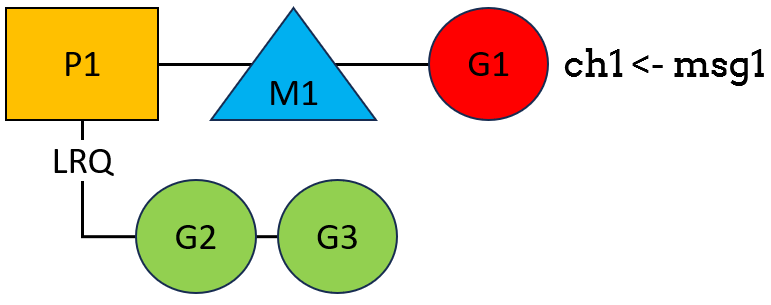
\includegraphics[scale=0.5]{figures/GoroutineChannel1.png}
	\caption{Go Channel-Kommunikation: Goroutine 1 wird ausgeführt und blockiert}
	\label{fig:GoroutineChannel1}
\end{figure}

In der Abbildung ist die oben beschriebene Ausgangssituation zu sehen. P1 führt aktuell G1 aus. G1 möchte die Nachricht \texttt{msg1} an den Channel \texttt{ch1} senden. Da es aktuell keinen Empfänger gibt blockiert G1 und wechselt in den Status Waiting. Dies registriert der Scheduler und entnimmt G1 aus P1, wie in der nächsten Abbildung deutlich wird.

\begin{figure}[H]
	\centering
	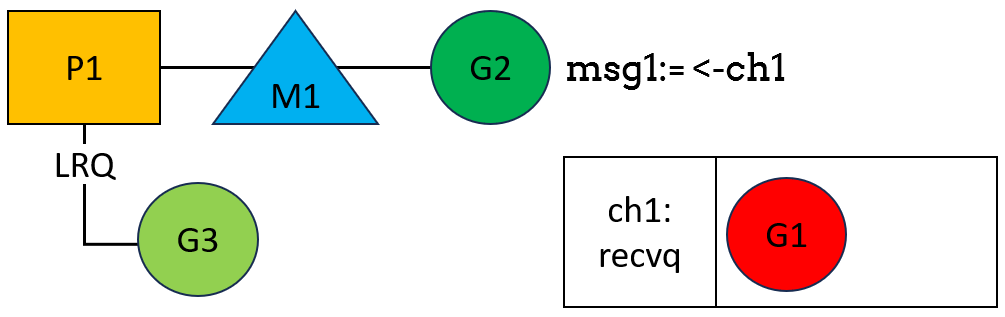
\includegraphics[scale=0.5]{figures/GoroutineChannel2.png}
	\caption{Go Channel-Kommunikation: Goroutine 1 wird entfernt, Goroutine 2 wird ausgeführt}
	\label{fig:GoroutineChannel2}
\end{figure}

Der Scheduler hat G1 aus P1 entfernt und der Empfänger-Warteschlange \texttt{recvq} des Channels \texttt{ch1} zugewiesen. Dort wartet G1 auf einen Empfänger für die Nachricht. Da P1 jetzt keine Goroutine mehr ausführt, entnimmt er die vorderste Goroutine aus seiner LRQ und beginnt mit der Bearbeitung. In diesem Fall ist dies G2. Dafür wird weiterhin der Betriebssystem Thread M1 genutzt dem P1 bereits zugewiesen war. Der Status von G2 wird dementsprechend von runnable auf running geändert. G2 wiederum empfängt eine Nachricht vom Channel \texttt{ch1}, was zur Folge hat, dass G1 nicht länger blockiert ist, wie in der folgenden Abbildung zu sehen ist.

\begin{figure}[H]
	\centering
	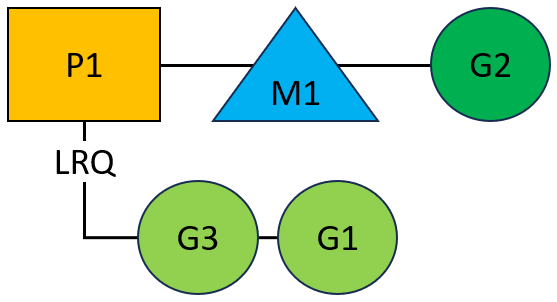
\includegraphics[scale=0.5]{figures/GoroutineChannel3.png}
	\caption{Go Channel-Kommunikation: Goroutine 1 ist nicht mehr blockiert und wird in die LRQ verschoben}
	\label{fig:GoroutineChannel3}
\end{figure}

Da G2 die Nachricht von G1 empfangen hat ist G1 nicht mehr blockiert und wechselt auf den Status Runnable. Deshalb verschiebt der Scheduler G1 in die LRQ von P1.

Diese Beispiel hat verdeutlicht wie der Scheduler mit einer Goroutine umgeht die aufgrund von Channel-Kommunikation blockiert. In der Praxis hat ein System jedoch meist mehr als einen Prozessorkern, was dem Go-Scheduler zusätzliche Möglichkeiten zur Optimierung der Ausführung bietet. Dies wird im Abschnitt Workstealing(\ref{subsubsec:workstealing}) genauer erläutert.

\subsubsection{Systemaufrufe}

In dem folgenden Beispiel wird gezeigt wie der Scheduler mit Systemaufrufen innerhalb von Goroutinen umgeht. In diesem Beispiel gehen wir wieder von einem System mit einem Prozessorkern aus. Deshalb gibt es auch wieder nur einen logischen Prozessor P1. Dieser führt die Goroutine G1 auf dem Betriebssystemthread M1 aus. Außerdem wartet eine zweite Goroutine G2 in der LRQ von P1 darauf ausgeführt zu werden. Schlussendlich gibt es noch einen zweiten untätigen Betriebssystemthread M2, der aktuell nicht genutzt wird.

\begin{figure}[H]
	\centering
	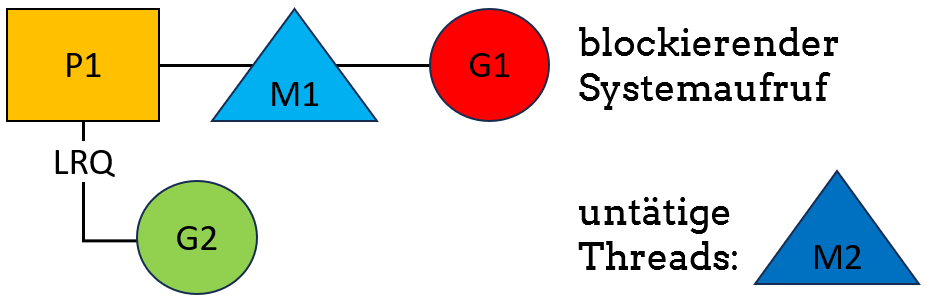
\includegraphics[scale=0.5]{figures/GoroutineSystemaufrufe1.png}
	\caption{Go Systemaufrufe: Goroutine 1 ist auf Grund eines Systemaufrufs blockiert}
	\label{fig:GoroutineSystemaufrufe1}
\end{figure}

G1 führt einen Systemaufruf aus, der dazu führt, dass G1 blockiert. Dies könnte beispielsweise eine I/O-Operation sein. Go hat keine direkte Kontrolle über die Ausführung von Systemaufrufen auf Betriebssystemebene. Sobald ein Systemaufruf initiiert wird, liegt die Kontrolle beim Betriebssystem. Deshalb blockiert nicht nur G1 sondern auch der ausführende Betriebssystemthread M1. Damit P1 weiterhin ausgelastet ist, werden sowohl G1 als auch M1 vom Scheduler freigegeben. P1 wird dann ein neuer Betriebssystemthread, in diesem Fall M2, zugewiesen und P1 kann die nächste Goroutine aus der LRQ ausführen, in diesem Fall G2.

\begin{figure}[H]
	\centering
	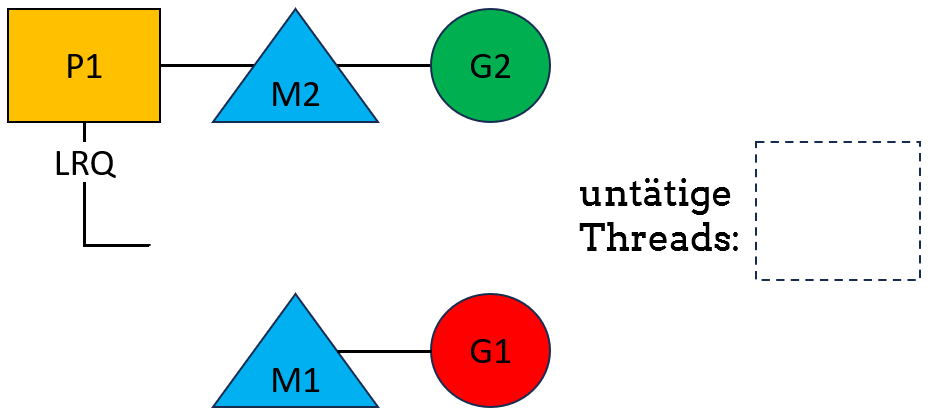
\includegraphics[scale=0.5]{figures/GoroutineSystemaufrufe2.png}
	\caption{Go Systemaufrufe: Goroutine 1 wird zusammen mit dem Betriebssystemthread M1 aus P1 entfernt, Goroutine 2 wird auf M2 ausgeführt}
	\label{fig:GoroutineSystemaufrufe2}
\end{figure}

Wenn G1 nicht mehr blockiert ist, überprüft der Scheduler, ob es einen freien logischen Prozessor gibt, der G1 auf M1 ausführen kann. In diesem Beispiel ist P1 aber mit der Ausführung von G2 beschäftigt. Deshalb wird G1 in die Global Run Queue (GRQ) verschoben. Dort gespeicherte Goroutinen werden von den logischen Prozessoren abgearbeitet sollte ihre eigene LRQ leer sein. M1 hingegen wird zu einem untätigen Thread.

\begin{figure}[H]
	\centering
	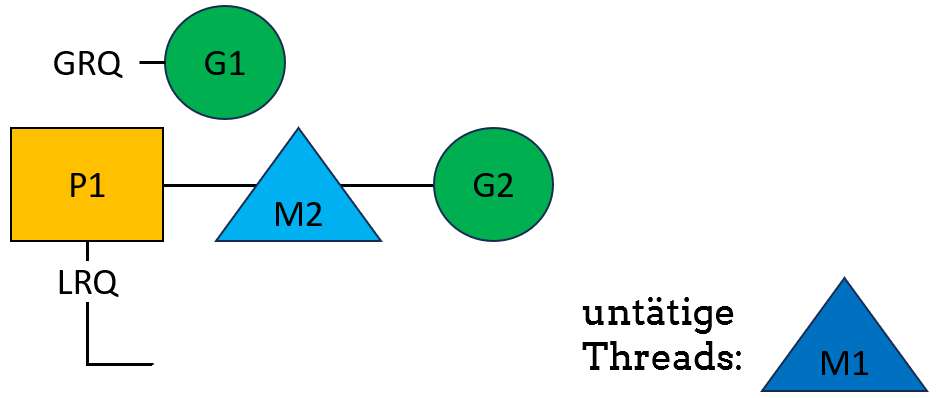
\includegraphics[scale=0.5]{figures/GoroutineSystemaufrufe3.png}
	\caption{Go Systemaufrufe: Goroutine 1 ist nicht mehr blockiert und wird in die GRQ verschoben}
	\label{fig:GoroutineSystemaufrufe3}
\end{figure}

Der Vorteil diese Verfahrens ist, dass die logischen Prozessoren nicht mit den Goroutinen blockieren. Sie können weiterhin Goroutinen ausführen. Jedoch wird für jeden Systemaufruf ein eigener Betriebssystemthread benötigt.

\subsubsection{Netzwerk-Kommunikation}

Eine weitere Kategorie häufig blockierender Operationen ist die Kommunikation über Netzwerke. Für diesen Fall stellt Go den Net Poller\cite{netpoll2024} zur Verfügung. Er ist ein spezieller Goroutinen-Scheduler, der für die effiziente Verwaltung von Netzwerk-I/O-Operationen zu\-stän\-dig ist. Er nutzt betriebssystemspezifische Mechanismen wie \texttt{epoll} (Linux), \texttt{kqueue} (BSD) oder \texttt{IOCP} (Windows), um asynchrone I/O-Operationen zu ermöglichen.

Wenn eine Goroutine eine potenziell blockierende Netzwerkoperation durchführt (z.B. Lesen von einem Socket), übergibt sie die Kontrolle an den Net Poller. Der Net Poller registriert die Operation beim Betriebssystem und überwacht sie asynchron ohne einen OS-Thread zu blockieren. Während der Net Poller auf die Fertigstellung der I/O-Operation wartet, kann der Go-Scheduler andere Goroutinen auf dem verfügbaren OS-Thread ausführen. Sobald die I/O-Operation abgeschlossen ist, benachrichtigt das Betriebssystem den Net Poller. Der Net Poller setzt die ursprüngliche Goroutine zur Ausführung fort, sobald ein Thread verfügbar ist.

Der Net Poller ermöglicht es, eine große Anzahl von gleichzeitigen Netzwerkverbindungen mit einer begrenzten Anzahl von Betriebssystemthreads zu verwalten. Durch die Vermeidung von blockierten Betriebssystemthreads wird die CPU-Auslastung optimiert. Programmierer können blockierende I/O-Operationen in Goroutinen schreiben, ohne sich um die zugrunde liegende asynchrone Implementierung kümmern zu müssen, da der Net Poller tief in die Go-Laufzeitumgebung integriert ist. Er arbeitet eng mit dem Goroutine-Scheduler zusammen, um eine nahtlose Integration von Netzwerk-I/O und Goroutinen-Ausführung zu gewährleisten. 

\subsubsection{Work-Stealing}
\label{subsubsec:workstealing}

Dieser Abschnitt zeigt wie der Work-Stealing-Algorithmus im Goroutinen-Scheduler funktioniert. Er sorgt für eine effiziente Verteilung der Arbeitslast zwischen den verfügbaren logischen Prozessoren (P). Jeder Prozessor (P) hat eine eigene lokale Warteschlange (LRQ) für Goroutinen. Neue Goroutinen werden normalerweise in die lokale Warteschlange des erzeugenden P gelegt. Ein P arbeitet primär an Goroutinen aus seiner eigenen lokalen Warteschlange. In diesem Beispiel gibt es zwei Prozessorkerne und damit zwei logische Prozessoren P1 und P2. Diese arbeiten die ihnen zugewiesenen Goroutinen ab.

\begin{figure}[H]
	\centering
	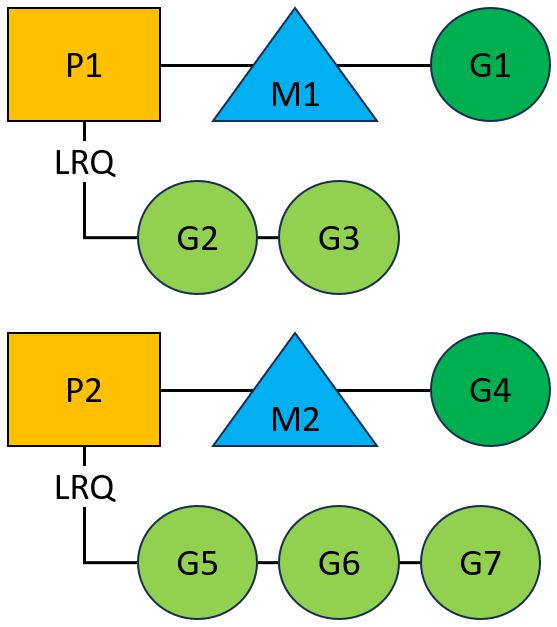
\includegraphics[scale=0.5]{figures/GoroutineWorkstealing1.png}
	\caption{Go Work-Stealing: P1 und P2 führen Goroutinen aus und haben gefüllte LRQs}
	\label{fig:GoroutineWorkstealing1}
\end{figure}

Wenn ein P keine Goroutinen mehr in seiner LRQ hat, versucht er, Goroutinen zu ``stehlen''. Er wählt zufällig einen anderen P aus und versucht, Goroutinen aus dessen LRQ zu entnehmen. In diesem Fall hat P1 alle seine Goroutinen abgearbeitet während P2 immer noch beschäftigt ist.

\begin{figure}[H]
	\centering
	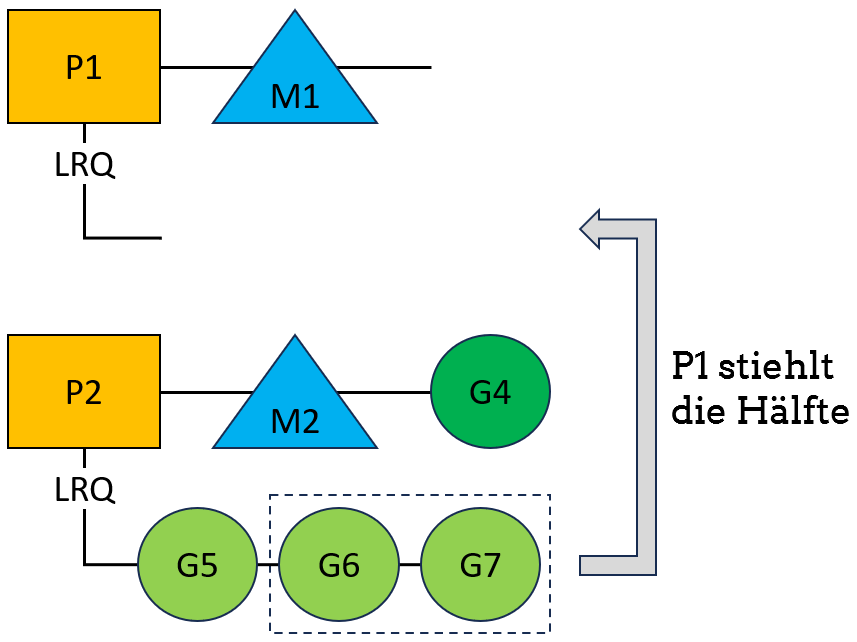
\includegraphics[scale=0.5]{figures/GoroutineWorkstealing2.png}
	\caption{Go Work-Stealing: P1 hat keine Goroutinen mehr und stiehlt die Hälfte der Goroutinen aus der LRQ von P2}
	\label{fig:GoroutineWorkstealing2}
\end{figure}

Deshalb stiehlt P1 die hintere Hälfte der LRQ von P2 und verschiebt sie in seine eigene LRQ. Wenn das Stehlen von anderen Ps nicht erfolgreich ist, greift der P auf die GRQ zurück.

Der Work-Stealing-Algorithmus ist ein Schlüsselelement, das zur hohen Effizienz und Skalierbarkeit von Go's Nebenläufigkeitsmodell beiträgt. Er ermöglicht es, eine große Anzahl von Goroutinen effizient auf einer begrenzten Anzahl von Betriebssystem-Threads zu verwalten.

\subsection{Goroutinen-Programmiermuster}

Um das volle Potenzial von Goroutinen auszuschöpfen und typische Herausforderungen der nebenläufigen Programmierung zu bewältigen, haben sich in der Go-Community verschiedene Programmiermuster (Pattern) etabliert. Die Verwendung dieser Muster trägt dazu bei, komplexe Probleme in überschaubare Teilaufgaben zu zerlegen und die Kommunikation zwischen Goroutinen zu strukturieren. Die im Folgenden vorgestellten Programmiermuster stammen dabei aus den Vorträgen ''Go Concurrency Patterns''\cite{Pike2012} und ''Advanced Go Concurrency Patterns''\cite{Ajmani2013}.

\subsubsection{Generator-Programmiermuster}
\label{subsubsec:generator}

Das Generator-Muster ermöglicht das Erstellen von Funktionen, die Sequenzen von Werten produzieren, ohne alle Werte auf einmal im Speicher zu halten. Stattdessen werden die Werte bei Bedarf generiert und über einen Channel zurückgegeben. Bei dem folgenden Code-Beispiel handelt es sich um eine Modifizierung des Codes aus dem Channel-Abschnitt (\ref{subsec:channel}).

\begin{lstlisting}[language=Go,extendedchars=true]
	package main
	
	import (
		"fmt"
	)

	// Generator-Funktion mit Namensparameter
	func helloCounter(name string) <-chan string {
		ch := make(chan string)
		// Starten der Goroutine
		go func() {
			for i := 0; i < 5; i++ {
				ch <- fmt.Sprintf("Hallo %s, %d!\n", name, i)
			}
			close(ch)
		}()
		return ch
	}

	func main() {
		philipp := helloCounter("Philipp")
		michael := helloCounter("Michael")
		for i := 0; i < 5; i++{
			fmt.Print(<-philipp)
			fmt.Print(<-michael)
		}
	}
\end{lstlisting}
Konsolenausgabe:
\begin{lstlisting}[frame=shadowbox, rulecolor=\color{black}, backgroundcolor=\color{gray!10}]
	Hallo Philipp, 0!
	Hallo Michael, 0!
	Hallo Philipp, 1!
	Hallo Michael, 1!
	Hallo Philipp, 2!
	Hallo Michael, 2!
	Hallo Philipp, 3!
	Hallo Michael, 3!
	Hallo Philipp, 4!
	Hallo Michael, 4!
\end{lstlisting}

Die auffälligste Veränderung ist, dass die Funktion \texttt{helloCounter} in der \texttt{main}-Funktion nicht mehr mit dem Schlüsselwort \texttt{go} als Goroutine gestartet werden muss. Stattdessen wird die Goroutine in der Funktion \texttt{helloCounter} intern gestartet. Außerdem wird auch der Channel von \texttt{helloCounter} erstellt und als Rückgabewert zurückgegeben. Das hat den Vorteil, dass sich, wie im Beispiel gezeigt, leicht mehrere Instanzen der Generatorfunktion nebenläufig starten lassen. Im Prinzip lässt sich eine Generatorfunktion als Service betrachten, bei dem sich der Anwender nicht mehr um die Nebenläufigkeit kümmern muss, da sie bereits intern sichergestellt wurde.

\subsubsection{Fan-In-Programmiermuster}

Die Aufgabe einer Fan-In-Funktion ist es, Ausgaben mehrerer Goroutinen zu sammeln und sie in einem einzigen Datenstrom zusammenzuführen. Durch die Zusammenführung mehrerer Datenströme in einem einzelnen Kanal wird die Verarbeitung der Ergebnisse effizienter gestaltet. In der Praxis wird die Fan-In-Funktion oft in Szenarien eingesetzt, wo Daten parallel verarbeitet werden müssen und die Ergebnisse anschließend zusammengeführt werden sollen, wie beispielsweise bei verteilten Berechnungen oder bei der Verarbeitung großer Datenmengen. Das nachfolgende Beispiel stellt eine Modifizierung des Codes aus dem Generator-Muster Abschnitt (\ref{subsubsec:generator}) dar.

\begin{lstlisting}[language=Go,extendedchars=true]
	func fanIn(ch1 <-chan string, ch2 <-chan string) <-chan string {
		new_ch := make(chan string)
		go func() {
			for {
				select {
					case s, ok := <-ch1:
					if !ok {
						ch1 = nil
						break
					}
					new_ch <- s
					case s, ok := <-ch2:
					if !ok {
						ch2 = nil
						break
					}
					new_ch <- s
				}
				if ch1 == nil && ch2 == nil {
					close(new_ch)
					return
				}
			}
		}()
		return new_ch
	}

	func main() {
		ch := fanIn(helloCounter("Philipp"), helloCounter("Michael"))
		for msg := range ch {
			fmt.Println(msg)
		}
	}
\end{lstlisting}
Mögliche Konsolenausgabe:
\begin{lstlisting}[frame=shadowbox, rulecolor=\color{black}, backgroundcolor=\color{gray!10}]
	Hallo Michael, 0!
	Hallo Michael, 1!
	Hallo Michael, 2!
	Hallo Michael, 3!
	Hallo Philipp, 0!
	Hallo Philipp, 1!
	Hallo Philipp, 2!
	Hallo Philipp, 3!
	Hallo Philipp, 4!
	Hallo Michael, 4!
\end{lstlisting}

In dem Beispiel wurde der Code um eine Fan-In-Funktion erweitert. Dieser Funktion werden in der \texttt{main}-Funktion die beiden Channels der \texttt{helloCounter}-Funktionen übergeben. Die Aufgabe der Fan-In-Funktion ist es, die Ausgaben der beiden Channels zusammenzufassen und in einem neuen Channel (\texttt{new\_ch}) gebündelt an die \texttt{main}-Funktion weiterzugeben. Dafür wird in der Fan-In-Funktion das Generator-Muster verwendet. Es wird innerhalb der Funktion eine Goroutine gestartet. In der Goroutine wird eine \texttt{select}-Anweisung verwendet um auf beiden Channels parallel auf eine Antwort zu warten. Diese Antworten werden dann auf den \texttt{new\_ch} weiter geleitet. Dies geschieht so lange, bis beide Channels der \texttt{helloCounter}-Funktionen geschlossen sind. Dann wird auch der \texttt{new\_ch} geschlossen. Der Vorteil der Verwendung einer Fan-In-Funktion in der \texttt{main}-Funktion wird schnell deutlich. Dadurch ist es möglich mehrere Nachrichten hintereinander von der gleichen \texttt{helloCounter}-Funktion zu empfangen. Außerdem muss in der \texttt{main}-Funktion auch nur noch ein Channel verarbeitet werden. 

Als Gegenstück zum Fan-In-Muster gibt es das Fan-Out-Muster. Bei diesem werden Nachrichten aus einer einzelnen Quelle auf mehrere Goroutinen verteilt.

\subsubsection{Closing Channels-Programmiermuster}
\label{subsubsec:closingchannel}

Das Closing Channels-Muster ist ein wichtiges Konzept in Go, um Goroutinen sauber zu beenden und Ressourcen freizugeben. Das grundlegende Prinzip lautet: Der Sender eines Channels sollte den Channel schließen, nicht der Empfänger. Dies verhindert Ausnahmen (Panic) durch das Senden auf bereits geschlossene Kanäle. Das folgende Beispiel zeigt eine mögliche Implementierung des Closing Channels-Muster:

\begin{lstlisting}[language=Go,extendedchars=true]
package main

import (
	"fmt"
	"time"
)

func worker(id int, done <-chan struct{}, c <-chan int) {
	for {
		select {
			case <-done:
			fmt.Printf("Worker %d: Beende Arbeit\n", id)
			return
			case value := <-c:
			fmt.Printf("Worker %d: Verarbeite Wert %d\n", id, value)
			time.Sleep(time.Second) // Simuliere Verarbeitungszeit
		}
	}
}

func main() {
	done := make(chan struct{}) // Closing Channel
	c := make(chan int)
	
	// Starte drei Worker
	for i := 1; i <= 3; i++ {
		go worker(i, done, c)
	}
	
	// Sende Werte an die Worker
	for i := 1; i <= 5; i++ {
		c <- i
		fmt.Printf("Hauptroutine: Sende Wert %d\n", i)
		time.Sleep(500 * time.Millisecond) // Kurze Pause zwischen den Sendungen
	}
	
	fmt.Println("Hauptroutine: Beende alle Worker")
	close(done) // Signal zum Beenden senden
	
	// Warte kurz, damit die Worker-Ausgaben sichtbar sind
	time.Sleep(2 * time.Second)
}
\end{lstlisting}
Mögliche Konsolenausgabe:
\begin{lstlisting}[frame=shadowbox, rulecolor=\color{black}, backgroundcolor=\color{gray!10}]
	Hauptroutine: Sende Wert 1
	Worker 1: Verarbeite Wert 1
	Hauptroutine: Sende Wert 2
	Worker 3: Verarbeite Wert 2
	Hauptroutine: Sende Wert 3
	Worker 2: Verarbeite Wert 3
	Hauptroutine: Sende Wert 4
	Worker 1: Verarbeite Wert 4
	Hauptroutine: Sende Wert 5
	Worker 3: Verarbeite Wert 5
	Hauptroutine: Beende alle Worker
	Worker 2: Beende Arbeit
	Worker 1: Beende Arbeit
	Worker 3: Beende Arbeit
\end{lstlisting}

In der \texttt{main}-Funktion wird ein neuer separater Channel mit dem Namen \texttt{done} erstellt. Dies ist der so genannte Closing Channel. Danach werden drei \texttt{worker}-Goroutinen ge\-star\-tet. Diese erhalten Werte über den Channel \texttt{c} und geben sie auf der Konsole aus. Nachdem die Hauptroutine alle Werte gesendet hat schließt sie den Closing Channel. Dies signalisiert den  \texttt{worker}-Goroutinen, dass keine weiteren Werte gesendet werden und sie beenden sich selbst.

\subsection{Zusammenfassung: Goroutinen}

Bei Goroutinen handelt es sich um leichtgewichtige Threads, die nebenläufige Ausführungen ermöglichen. Sie lassen sich durch das Schlüsselwort \texttt{go} starten und laufen unabhängig von der Hauptfunktion, wobei sie einen gemeinsamen Adressraum teilen. Die Kommunikation und Synchronisation zwischen Goroutinen erfolgt über Channels, die den Datenaustausch ermöglichen. Die Go-Laufzeitumgebung enthält einen Scheduler, der Goroutinen effizient verwaltet. Um eine ausgewogene Auslastung der Prozessoren zu gewährleisten, nutzt der Scheduler verschiedene Warteschlangen(LRQ und GRQ) und einen Work-Stealing-Algorithmus. Verschiedene Programmiermuster, wie das Fan-In-Muster und das gezielte Schließen von Channels, unterstützen eine strukturierte Handhabung der Nebenläufigkeit und optimieren die Gesamtleistung der Programme.

\section{Vergleich der Konzepte}

Im Folgenden werden die Erkenntnisse, die über Java Platform Threads, Java Virtual Threads, Kotlin Coroutinen und Go Goroutinen gesammelt wurden, miteinander verglichen, um sowohl Gemeinsamkeiten als auch Unterschiede hervorzuheben.

\subsubsection{Unterstützte Sprachen}

Platform Threads sind in Java, Kotlin und anderen JVM-Sprachen verfügbar, was ihre breite Anwendbarkeit unterstreicht. Virtual Threads hingegen sind eine neuere Entwicklung und stehen ab Java Version 21 zur Verfügung. Kotlin Coroutinen sind spezifisch für die Kotlin-Sprache konzipiert, während Goroutinen exklusiv in Go implementiert sind.

\subsubsection{Ausführungskontrolle und Blockierverhalten}

Der Mechanismus zur Ausführungskontrolle variiert stark zwischen den Konzepten. Platform Threads nutzen betriebssystembasiertes Scheduling, was zu einer direkten Blockierung des BS-Threads führt. Im Gegensatz dazu verwenden Virtual Threads, Coroutinen und Goroutinen fortschrittlichere Mechanismen, die es ermöglichen, den BS-Thread freizugeben, wenn eine Operation blockiert. Virtual Threads und Kotlin Coroutinen basieren auf Continuations, während Go einen eigenen Goroutinen-Scheduler implementiert.

\subsubsection{Thread-Pool-Nutzung und Ressourcenverbrauch}

Auch bei der Thread-Pool-Nutzung zeigen sich Unterschiede: Platform Threads und Coroutinen erfordern eine explizite Nutzung, während Virtual Threads und Goroutinen dies implizit handhaben. Der Ressourcenverbrauch ist bei Platform Threads deutlich höher (schwergewichtig), während die anderen drei Konzepte als leichtgewichtig gelten.

\subsubsection{Stackgröße und maximale Anzahl}

Die Stackgröße variiert erheblich, von großen Stacks bei Platform Threads (oft 1 MB oder mehr), bis zu sehr kleinen bei Virtual Threads und Go Goroutinen. Kotlin Coroutinen nutzen keinen eigenen Stack, sondern den Hauptstack kurzzeitig. Diese Unterschiede wirken sich direkt auf die maximale Anzahl aus, die bei Platform Threads auf einige tausend begrenzt, bei den anderen Konzepten mit mehreren Millionen jedoch sehr hoch ist.

\subsubsection{Synchronisationsmechanismen}

Die Synchronisationsmechanismen reichen von klassischen Locks, Monitoren und Futures bei Platform und Virtual Threads bis zu spezialisierten Konzepten wie suspend und Scope bei Kotlin Coroutinen oder Channels bei Go Goroutinen. 

\begin{table}[h]
	\centering
	\renewcommand{\arraystretch}{1.2}
	\begin{tabularx}{\textwidth}{L{4cm}Y Y Y Y}
		\toprule
		\rowcolor{gray!20}
		\textbf{Eigenschaft} & \textbf{\makecell[l]{Java \\ Platform \\ Threads}} & \textbf{\makecell[l]{Java \\ Virtual \\ Threads}} & \textbf{\makecell[l]{Kotlin \\ Coroutinen}} & \textbf{\makecell[l]{Go \\ Goroutinen}} \\
		\midrule
		Unterstützte Sprachen & Java, Kotlin, JVM-Sprachen & Java (ab Version 21) & Kotlin & Go \\
		\rowcolor{gray!10}
		Mechanismus zur Ausführungskontrolle & BS-basiertes Scheduling & Continuations (Scheduling durch JVM) & Continuations (Kotlin Runtime) & Goroutinen-Scheduler (Go Runtime) \\
		Blockierverhalten & Blockiert BS-Thread & Gibt BS-Thread frei & Gibt BS-Thread frei & Gibt BS-Thread frei \\
		\rowcolor{gray!10}
		Thread-Pool-Nutzung & Explizit & Implizit & Explizit (Dispatcher) & Implizit \\
		Ressourcenverbrauch & \makecell[l]{Schwer-\\gewichtig} & \makecell[l]{Leicht-\\gewichtig} & \makecell[l]{Leicht-\\gewichtig} & \makecell[l]{Leicht-\\gewichtig} \\
		\rowcolor{gray!10}
		Stackgröße & Groß (oft 1 MB oder mehr) & Klein (oft ein paar KB) & Kein eigener Stack, nutzt Hauptstack kurz & Klein (einige KB, wächst dynamisch) \\
		Maximale Anzahl & Begrenzt & Hoch & Sehr hoch & Sehr hoch \\
		\rowcolor{gray!10}
		\makecell[l]{Synchronisations-\\mechanismen} & Locks, Monitore, Future & Locks, Monitore, Future & suspend, Scope & Channels \\
	\end{tabularx}
	\caption{Vergleich von Thread-Abstraktionen in verschiedenen Programmiersprachen}
	\label{tab:thread-comparison}
\end{table}

Mit diesem Kapitel endet der theoretische Teil der Masterarbeit, in dem die unterschiedlichen Konzepte zur Thread-Abstraktion ausführlich vorgestellt und miteinander verglichen wurden. Die behandelten Technologien – Java Platform Threads, Java Virtual Threads, Kotlin Coroutinen und Go Goroutinen – wurden hinsichtlich ihrer Funktionsweise, Stärken und Schwächen gegenübergestellt. Diese theoretische Grundlage bildet das Fundament für den nun folgenden praktischen Teil der Arbeit, in dem die vorgestellten Aussagen durch Benchmarks überprüft werden. Ziel ist es, die Leistungsfähigkeit und Skalierbarkeit der Konzepte unter realistischen Bedingungen zu verifizieren oder gegebenenfalls zu falsifizieren.



\chapter{Testaufbau}

Das folgende Kapitel beschreibt den Testaufbau für die praktische Umsetzung der Leistungsanalyse der verschiedenen Thread-Abstraktionen in Java, Kotlin und Go. 

Um eine fundierte und aussagekräftige Bewertung der Per\-for\-mance\-un\-ter\-schiede zu erzielen, wurde in Rahmen dieser Masterarbeit ein sorgfältig konzipierter Testaufbau entwickelt. Dieser Aufbau gewährleistet nicht nur die Vergleichbarkeit der Ergebnisse zwischen den verschiedenen Programmiersprachen und ihren Thread-Implementierungen, sondern stellt auch die Reproduzierbarkeit der Messungen sicher.

In den folgenden Abschnitten wird zunächst die verwendete Testumgebung, einschließlich der Hardware- und Software-Konfiguration, beschrieben. Anschließend werden die für die Leistungsanalyse relevanten Performancefaktoren erläutert und begründet. Diese Faktoren bilden die Grundlage für die quantitative Bewertung der verschiedenen Thread-Abs\-trak\-tio\-nen. Abschließend werden die speziell für diese Untersuchung entwickelten Werkzeuge zur Datenerhebung vorgestellt. Diese maßgeschneiderten Tools ermöglichen eine präzise und konsistente Erfassung der Leistungsdaten über alle getesteten Implementierungen hinweg.

\section{Testumgebung}

Um eine konsistente und reproduzierbare Testumgebung für die Leistungsanalyse der verschiedenen Thread-Abs\-trak\-tio\-nen zu gewährleisten, wurde eine spezifische Hard- und Soft\-ware-Konfiguration verwendet. Diese Konfiguration wurde für alle durchgeführten Benchmarks beibehalten, um vergleichbare Ergebnisse zu erzielen.

Alle Tests wurden in einer kontrollierten Umgebung durchgeführt, wobei darauf geachtet wurde, dass keine anderen ressourcenintensiven Prozesse parallel liefen. Das System wurde vor jedem Testlauf neu gestartet, um konsistente Ausgangsbedingungen zu gewährleisten. Zudem wurden alle Netzwerkverbindungen deaktiviert, um mögliche Interferenzen durch externe Faktoren zu minimieren.

\newpage
\subsection{Hardware}

\begin{itemize}
	\item \textbf{Prozessor:} Intel(R) Core(TM) i5-8300H CPU @ 2.30GHz
	\item[] \hspace{0.8cm}\textbf{Kerne:} 4 physische Kerne, 8 logische Prozessoren
	\item[] \hspace{0.8cm}\textbf{Basistakt:} 2.30GHz
	\item \textbf{Arbeitsspeicher:} 16,0 GB (15,9 GB verwendbar)
	\item \textbf{Festplatte:} SSD 256 GB
\end{itemize}

\subsection{Software}

\begin{itemize}
	\item \textbf{Betriebssystem:} Microsoft Windows 11 Home (Version 26100.2161, 64-Bit)
	\item \textbf{Java Development Kit (JDK):} openjdk 21.0.2
	\item \textbf{Kotlin JVM:} 1.9.22
	\item \textbf{Go:} 1.23.3
	\item \textbf{Python:} 3.12.5
	\item \textbf{Docker:} 27.3.1
	\item \textbf{PostgreSQL:} 17.2
	\item \textbf{PostgREST:} 12.2.3
\end{itemize}

\section{Performancefaktoren}

Bei der Analyse und dem Vergleich verschiedener Thread-Abstraktionen ist es entscheidend, aussagekräftige und messbare Kriterien heranzuziehen. Diese Kriterien, die als Performancefaktoren bezeichnet werden, ermöglichen eine objektive Bewertung der Leistungsfähigkeit und Effizienz der unterschiedlichen Implementierungen. In dieser Masterarbeit liegt der Fokus auf vier Faktoren: Zeitmessung, CPU-Auslastung, Arbeitsspeicherverbrauch und Thread-Anzahl. Jeder dieser Faktoren beleuchtet einen spezifischen Aspekt der Leistung und trägt zu einem umfassenden Verständnis der Stärken und Schwächen der jeweiligen Thread-Abstraktionen bei. Die Performancefaktoren ermöglichen es, die Effizienz, Skalierbarkeit und Ressourcennutzung der verschiedenen Thread-\-Imple\-mentie\-rungen detailliert zu untersuchen und zu vergleichen. Im Folgenden wird jeder dieser Faktoren genauer betrachtet und erläutert.

\subsubsection{Zeitmessung}

Die Ausführungszeit ist einer der wichtigsten Indikatoren für die Leistungsfähigkeit der Thread-Abstraktionen. Durch präzise Zeitmessungen können verschiedene Implementierungen objektiv miteinander verglichen werden, um die effizienteste Lösung zu identifizieren. In der Praxis ist die Einhaltung von zeitlichen Vorgaben in Systemen mit Echtzeitanforderungen maßgebend. Durch Zeitmessungen mit unterschiedlichen Eingabegrößen oder Lastszenarien kann die Skalierbarkeit eines Systems analysiert werden. So lässt sich abschätzen, wie sich die Leistung bei wachsenden Anforderungen entwickelt.

\subsubsection{CPU-Auslastung}

Die CPU-Auslastung gibt direkten Aufschluss darüber, wie effizient die verfügbaren Prozessorressourcen von den Threads genutzt werden. Eine hohe Auslastung deutet auf eine gute Ausnutzung der Rechenkapazität hin, während eine niedrige Auslastung auf Ineffizienzen oder Engpässe in anderen Bereichen hinweisen kann. Durch die Analyse der CPU-Auslastung lässt sich der Grad der Parallelisierung eines multithreaded Systems beurteilen. Eine gleichmäßige Auslastung über mehrere Kerne hinweg zeigt, dass die Arbeitslast effektiv auf die verfügbaren Ressourcen verteilt wird.

Im zweiten Benchmark wird zusätzlich die CPU-Auslastung der PostgreSQL-Datenbank gemessen, die als Backend für die betrachteten Anwendungen dient.

\subsubsection{Arbeitsspeicherverbrauch}

Ein effizienter Umgang mit dem Arbeitsspeicher ist entscheidend für die Gesamtleistung eines multithreaded Programms. Jeder Thread benötigt Speicher für seinen Stack und andere thread-spezifische Daten. Ein hoher Speicherverbrauch kann zu einer Verlangsamung des Systems führen und die Anzahl der möglichen gleichzeitigen Threads begrenzen. Der Speicherverbrauch beeinflusst direkt die Skalierbarkeit eines multithreaded Programms. Ein geringer Speicherverbrauch pro Thread ermöglicht mehr gleichzeitige Threads, während ein hoher Speicherbedarf die maximale Anzahl der Threads und damit die Parallelisierung limitiert.  Außerdem führt ein steigender Speicherverbrauch auch zu steigenden Betriebskosten. Schließlich schont ein effizienter Speicherverbrauch die Systemressourcen, indem mehr verfügbarer Speicher für andere Prozesse und den Betriebssystem-Cache bleibt und die Belastung des Speichermanagements des Betriebssystems geringer ausfällt.

\subsubsection{Thread-Anzahl}

Die Anzahl der Betriebssystemthreads ist ein bedeutender Performancefaktor bei der Messung der Benchmarks. Betriebssystemthreads sind eine begrenzte Ressource. Jeder Thread benötigt Speicher und andere Systemressourcen, was bedeutet, dass eine zu hohe Anzahl von Threads zu Ressourcenengpässen führen und die Gesamtleistung des Systems beeinträchtigen kann. Mit steigender Anzahl von Threads erhöht sich auch der Aufwand für das Betriebssystem, diese zu verwalten und zu planen. Dieser erhöhte Scheduling-Overhead kann zu einem höheren CPU-Verbrauch für Verwaltungsaufgaben und häufigeren Kontextwechseln führen, was die Effizienz des Gesamtsystems beeinträchtigt. Ab einem bestimmten Punkt kann eine Erhöhung der Threadanzahl sogar zu Leistungseinbußen führen, da die Threads um begrenzte Ressourcen konkurrieren.

\section{Werkzeuge zur Datenerhebung}

Für die Durchführung der Benchmarks und die Erhebung der relevanten Performance\-daten wurden zwei speziell für diese Masterarbeit neu entwickelte Python-Skripte verwendet. Diese Skripte ermöglichen eine präzise und konsistente Messung der Leistungsparameter über alle getesteten Thread-Abstraktionen hinweg. Ein drittes Skript kann die so erhobenen Daten aggregieren und aus ihnen Graphen generieren.

\subsubsection{Überwachung: Mergesort}

Um den Mergesort-Benchmark durchzuführen und dabei die Performancedaten der unterschiedlichen Implementierungen zu sammeln, wurde das Python-Script \texttt{monitoring""Merge""sort.py} für diese Masterarbeit entwickelt.

Es startet die einzelnen Implementierungen mit vorher definierten Parametern, misst die Ausführungszeit in Sekunden sowie die Nutzung von CPU, Arbeitsspeicher und Threads während der Ausführung und speichert diese Daten in CSV-Dateien zur späteren Analyse. Das Skript ermöglicht es, verschiedene Algorithmen zu vergleichen, indem es für jede Implementierung die Leistung unter unterschiedlichen Bedingungen, wie zum Beispiel verschiedenen Maximal-Tiefen des Mergesort-Algorithmus, protokolliert. Eine genauere Aufschlüsselung der möglichen Parameter befinden sich in Abschnitt \ref{subsec:mergsortpara}.

Um die Performancefaktoren zu erfassen, nutzt das Skript mehrere Python-Bibliotheken und Funktionen. Ein zentraler Bestandteil ist die Bibliothek \texttt{psutil}, die die Möglichkeit bietet, einen Prozess anhand seiner Prozess-ID zu überwachen. Der Arbeitsspeicherverbrauch wird mit Hilfe der Funktion \texttt{.memory\_info().rss} gemessen. Für die Messung der Betriebssystem-Threads wird die Funktion \texttt{.num\_threads()} verwendet. Beide Funktionen geben den aktuellen Wert zum Zeitpunkt des Aufrufs zurück. Deshalb wurde die Abtastrate auf 0,2 Sekunden gesetzt. In der Praxis hat sich gezeigt, dass bei dieser Rate annähernd alle Wertveränderungen erfasst werden.

Zur Messung der CPU-Auslastung wird die Funktion \texttt{psutil.cpu\_count()} genutzt. Im Gegensatz zu den zuvor vorgestellten Funktionen handelt es sich hierbei um eine aggregierende Funktion, die die durchschnittliche CPU-Nutzung seit dem letzten Aufruf zurückgibt. Deshalb wurde der Messabstand zwischen den Aufrufen mit 2 Sekunden größer gewählt.

Um die Ausführungszeit zu messen, wird die \texttt{time}-Bibliothek von Python verwendet. Es wird die Gesamtzeit über alle Sortierungsdurchläufe hinweg gemessen. Dabei beginnt die Messung erst, nachdem die zu sortierende Liste importiert wurde und alle Aufwärmdurchläufe abgeschlossen sind, und endet, nachdem alle Sortierdurchläufe beendet wurden. Auch die anderen Messungen der anderen Parameter finden nur in diesem Zeitfenster statt. 

Abschließend werden die so erhobenen Rohdaten in entsprechenden CSV-Dateien gespeichert.

\subsubsection{Überwachung: Bank}
\label{subsubsec:monibank}

Für die Überwachung des Bank-Benchmarks wurde ein weiteres Python-Skript namens \texttt{monitoring""Bank.py} entwickelt.

Zu Beginn des Skripts wird die Java-Anwendung \texttt{bankDataGenerator.jar} (Abschnitt: \ref{para:datagenerator}) gestartet, diese erzeugt den für den Benchmark nötigen Datensatz, der von allen Implementierungen genutzt wird. 

Da die unterschiedlichen Implementierungen des Benchmarks in Docker Containern laufen (siehe Abschnitt \ref{para:docker} für den genauen Aufbau), wird im nächsten Schritt die Datei \texttt{docker-""compose\_""modify"".yaml} erzeugt. In dieser werden die für den Durchlauf wichtigen Parameter gesetzt, wie zum Beispiel die Anzahl der Accounts und Transaktionen oder die Wahl der Implementierung. Eine vollständige Auflistung der Parameter befindet sich in Abschnitt \ref{subsec:parabank}.

Anschließend wird der eigentliche Benchmark mit Hilfe der \texttt{docker-""compose\_""modify"".yaml} gestartet. Die Überwachung der Performancefaktoren kann in diesem Benchmark jedoch nicht mit der \texttt{psutil} Bibliothek durchgeführt werden, da dafür die Prozess ID nötig wäre, welche aber nicht auslesbar ist, da die Implementierungen in einem Docker Container laufen. Deshalb werden die Performancefaktoren: CPU-Auslastung, Arbeitsspeicherverbrauch und Thread-Anzahl in diesem Skript mit \texttt{docker stats} erhobenen. Die Abtastrate von \texttt{docker stats} liegt bei einer Sekunde. Da aber pro Messung auch einmal \texttt{docker inspect} aufgerufen wird ergibt sich eine faktische Abtastrate von zwei Sekunden. Dies hat sich als ausreichend erwiesen, da die Schwankungen zwischen den Messungen sehr gering sind und die Messungen lange laufen. 

Die Ausführungszeit kann erneut mit der \texttt{time}-Bibliothek gemessen werden. Für alle Performancefaktoren gilt erneut, die Messungen beginnen erst, wenn alle nötigen Daten importiert wurden und enden mit der Beendigung des Programms. Abschließend werden alle gesammelten Daten in CSV-Dateien gespeichert. 

\subsubsection{Datenaufbereitung}

Zur Aufbereitung und Visualisierung der erhobenen Daten aus den Benchmarks wurde ein drittes Python-Skript erstellt, das mit Hilfe der Bibliotheken \texttt{numpy}, \texttt{pandas}, und \texttt{matplotlib} die gesammelten Performance-Daten verarbeitet und in anschauliche Diagramme umwandelt. Dieses Skript liest die Messdaten aus den CSV-Dateien, berechnet für jeden Algorithmus die maximalen und durchschnittlichen Werte für verschiedene Performance-Kennzahlen und erstellt daraufhin eine Reihe von Balkendiagrammen, die die Leistung der verschiedenen Implementierungen veranschaulichen. Zusätzlich werden die so für die Diagramme aggregierten Daten in Tabellenform in CSV-Dateien gespeichert.

\chapter{Benchmarks}

\section{Benchmark 1: Mergesort}

\subsection{Motivation: Mergesort}
Mergesort eignet sich hervorragend als Benchmark für den Vergleich verschiedener Thread-Abstraktionen. Der Algorithmus basiert auf dem Teile-und-herrsche-Prinzip, was eine na\-tür\-li\-che Parallelisierung ermöglicht. Durch seine rekursive Struktur lässt sich Mergesort in kleinere, unabhängige Teilaufgaben zerlegen, die ideal für die parallele Verarbeitung geeignet sind. Dies macht den Algorithmus zu einem aussagekräftigen Testfall für die Effizienz und Skalierbarkeit verschiedener Nebenläufigkeitsimplementierungen.

Ein weiterer Vorteil von Mergesort als Benchmark ist seine vorhersehbare Zeitkomplexität von $\Theta(n\log{}n)$ für alle Eingabegrößen. Diese Eigenschaft ermöglicht es, die Leistung der verschiedenen Thread-Abstraktionen unter kontrollierten Bedingungen zu vergleichen. Zudem erfordert Mergesort sowohl Rechenoperationen als auch Speicherzugriffe, was eine umfassende Bewertung der Leistungsfähigkeit der untersuchten Technologien erlaubt.

Die Wahl von Mergesort als Benchmark hat tatsächlich auch praktische Relevanz, da der Algorithmus häufig in realen Anwendungen zum Einsatz kommt, insbesondere bei der Verarbeitung großer Datenmengen. Somit können die gewonnenen Erkenntnisse direkt auf praxisnahe Szenarien übertragen werden. Durch die Verwendung von Mergesort als Benchmark lassen sich wertvolle Einblicke in die Stärken und Schwächen der verschiedenen Thread-Abstraktionen und Nebenläufigkeitskonzepte gewinnen, was für die Auswahl der geeigneten Technologie in spezifischen Anwendungsfällen von großer Bedeutung ist.

\subsection{Theoretische Grundlagen: Mergesort}

Mergesort ist ein effizienter, auf dem Teile-und-herrsche-Prinzip basierender Sortieralgorithmus. Er wurde 1945 von John von Neumann entwickelt \cite{vonNeumann1945} und zeichnet sich durch seine stabile Sortierung und vorhersagbare Leistung aus.

\subsubsection{Funktionsweise}

Der Mergesort-Algorithmus lässt sich in zwei Hauptphasen unterteilen: die Teilungsphase und die Zusammenführungsphase.

In der Teilungsphase wird die zu sortierende Liste rekursiv in immer kleinere Teillisten zerlegt, bis jede Teilliste nur noch ein Element enthält. Dies geschieht, indem die Liste in der Mitte geteilt wird, wodurch zwei etwa gleich große Hälften entstehen.

In der Zusammenführungsphase werden die sortierten Teillisten schrittweise wieder zusammengeführt. Dabei werden jeweils zwei benachbarte, sortierte Teillisten zu einer größeren sortierten Liste verschmolzen. Dieser Prozess wird fortgesetzt, bis die gesamte Liste sortiert ist.

Die rekursive Natur des Mergesort-Algorithmus lässt sich anschaulich als Baumstruktur darstellen, die während der Teilungsphase entsteht. Die Wurzel des Baums repräsentiert die ursprüngliche, unsortierte Liste. Jeder innere Knoten stellt eine Teilung der Liste dar. Die Blätter des Baums sind die einzelnen Elemente der Liste. Die Tiefe des Baums entspricht der Anzahl der rekursiven Teilungen, die durchgeführt werden müssen, um zu einzelnen Elementen zu gelangen. Sie beträgt etwa $\log_2(n)$, wobei $n$ die Anzahl der Elemente in der ursprünglichen Liste ist.

Beim Aufstieg im Baum, also während der Zusammenführungsphase, werden die sortierten Teillisten schrittweise verschmolzen. Jede Ebene im Baum repräsentiert dabei einen Schritt im Sortierprozess, bei dem längere sortierte Sequenzen entstehen.

Diese Baumstruktur verdeutlicht nicht nur die Arbeitsweise des Algorithmus, sondern auch sein Parallelisierungspotenzial: Unterschiedliche Zweige des Baums können unabhängig voneinander bearbeitet werden, was eine effiziente parallele Implementierung ermöglicht.

\subsubsection{Komplexität}

Mergesort weist in allen Fällen (Best-Case, Average-Case und Worst-Case) eine Zeitkomplexität von $\Theta(n \log n)$ auf, wobei $n$ die Anzahl der zu sortierenden Elemente ist \cite{Cormen2022}. Dies macht Mergesort zu einem sehr effizienten Sortieralgorithmus, insbesondere für große Datenmengen. Außerdem sind dies sehr gute Voraussetzungen für die Eignung als Benchmark, da die zeitliche Performance nicht von dem Inhalt der zu verarbeitenden Daten abhängt.

Die Speicherkomplexität von Mergesort beträgt $\Theta(n)$, da zusätzlicher Speicherplatz für die temporären Teillisten benötigt wird. Dies kann bei sehr großen Datenmengen zu einem Nachteil werden.


\subsection{Implementierung: Mergesort}

In diesem Abschnitt wird die parallelisierte Implementierung von Mergesort vorgestellt. Als erstes wird der grundlegende Ansatz anhand von Pseudocode vorgestellt, danach wird auf die technischen Besonderheiten der einzelnen Implementierungen eingegangen, welche im Rahmen dieser Masterarbeit programmiert wurden.

\subsubsection{Basisimplementierung: Mergesort}
\label{subsubsec:implms}

Der grundlegende Ansatz zur Parallelisierung von Mergesort ist für alle vier Implementierungen gleich und basiert auf der Version aus \emph{Introduction to Algorithms} von Cormen et al. \cite[S. 775]{Cormen2022}, jedoch wurde er leicht modifiziert. Die Funktion wurde um zwei weitere Übergabeparameter erweiter: \texttt{currentDepth} und \texttt{maxDepth}. Mit diesen lässt sich mit Hilfe einer if-else-Bedingung regulieren, bis zu welcher Tiefe des durch die Rekursion enstehenden Baums parallelisiert werden soll. Die Rekursion wird auch danach weiter fortgesetzt, jedoch sequentiell.

\begin{algorithm}[H]
	\caption{P-MERGE-SORT(array, tempArray, left, right, currentDepth, maxDepth)}
	\begin{algorithmic}[1]
		\IF{$left \geq right$}
		\RETURN
		\ENDIF
		\STATE $mid \gets \lfloor (left + right) / 2 \rfloor$ \hfill // Mitte des Bereichs
		\IF{$currentDepth < maxDepth$} 
		\STATE \textbf{spawn} P-MERGE-SORT(array, tempArray, left, mid, currentDepth + 1, maxDepth)
		\STATE \textbf{spawn} P-MERGE-SORT(array, tempArray, mid + 1, right, currentDepth + 1, maxDepth)
		\STATE \textbf{sync} \hfill // Warte auf parallele Aufgaben
		\ELSE
		\STATE P-MERGE-SORT(array, tempArray, left, mid, currentDepth + 1, maxDepth)
		\STATE P-MERGE-SORT(array, tempArray, mid + 1, right, currentDepth + 1, maxDepth)
		\ENDIF
		\STATE MERGE(array, tempArray, left, mid, right) \hfill // Merge der Teilbereiche
	\end{algorithmic}
\end{algorithm}

Des weiteren gibt  es einen Vorschlag wie sich zusätzlich die merge-Funktion parallelisieren lässt \cite[S. 776-782]{Cormen2022}. In der Praxis hat sich jedoch gezeigt, dass der Vorschlag sogar zu einer Verschlechterung der Laufzeit führt, deshalb wurde statt dessen ein sequentieller Ansatz genutzt \cite[S. 36]{Cormen2022}. Das schlechtere Abschneiden der parallelen merge-Implementierung hat verschiedene Gründe. So bietet eine Parallelisierung von merge ab einer bestimmten Baumtiefe keinen Vorteil mehr, da die Mergesort-Funktion bereits parallelisiert wurde und  die CPU-Kerne ab einer bestimmten Baumtiefe bereits vollständig ausgelastet sind, sodass eine zusätzliche Parallelisierung von merge keinen weiteren Vorteil bringt. Außerdem entsteht Overhead für die Verwaltung der parallelen Aufgaben, sowie für die wiederholte Suche nach dem Pivot-Element.

\begin{algorithm}[H]
	\caption{MERGE(array, tempArray, left, mid, right)}
	\begin{algorithmic}[1]
		\STATE Kopiere $array[left..right]$ in $tempArray[left..right]$
		\STATE $i \gets left, j \gets mid + 1, k \gets left$
		\WHILE{$i \leq mid$ \AND $j \leq right$}
		\IF{$tempArray[i] \leq tempArray[j]$}
		\STATE $array[k] \gets tempArray[i]$
		\STATE $i \gets i + 1$
		\ELSE
		\STATE $array[k] \gets tempArray[j]$
		\STATE $j \gets j + 1$
		\ENDIF
		\STATE $k \gets k + 1$
		\ENDWHILE
		\STATE Kopiere verbleibende Elemente aus $tempArray[i..mid]$ nach $array[k..]$
	\end{algorithmic}
\end{algorithm}

Durch die Verwendung der sequentiellen merge-Implementierung kommt es jedoch zu einer Besonderheit bei der durchschnittlichen CPU-Auslastung. Diese liegt bei ungefähr 82\%. Der Grund dafür ist, dass auf höheren Baumebenen noch nicht genug Knoten vorhanden sind, um die CPU vollständig auszulasten. Auf der ersten Ebene gibt es nur einen Knoten, weshalb nur ein Kern genutzt werden kann. Auf der zweiten Ebene existieren zwei Knoten, was es ermöglicht, zwei Kerne zu verwenden, und auf der dritten Ebene gibt es vier Knoten, was vier Kerne beansprucht, und so weiter. Diese zunehmende Anzahl an Knoten führt dazu, dass mit jeder weiteren Ebene mehr CPU-Kerne aktiviert werden, bis irgendwann alle Kerne des Prozessors genutzt werden. Aufgrund dieser Struktur wird die CPU-Auslastung auf den höheren Ebenen des Baums nicht optimal maximiert, was zu einer durchschnittlichen Auslastung von etwa 82\% führt. Hinzu kommt, dass vor jedem Sortierdurchlauf erst eine Kopie der zu sortierenden Liste erstellt wird, damit die Ausgangsliste für weitere Sortierdurchläufe bestehen bleibt. 

Um sicherzustellen, dass der Performancevergleich zwischen den verschiedenen Mergesort-Implementierungen fair und konsistent ist, wird in allen Implementierungen die gleiche Liste verwendet. Diese Liste wird als Textdatei  gespeichert und in jede der Implementierungen importiert. Dies gewährleistet, dass jede Implementierung mit denselben Eingabedaten arbeitet und somit vergleichbare Ergebnisse erzielt werden.

\subsubsection{Platform Threads: Mergesort}

Die Implementierung für Java Platform Threads ist Teil der Anwendung \texttt{mergesort""Java"".jar}, und die relevante Klasse in dieser Implementierung ist \texttt{Mergesort""Platform""Threads"".java}.

Zur Verwaltung der Threads wird in dieser Implementierung ein ExecutorService verwendet, der über die Methode \texttt{.newCachedThreadPool()} einen Thread-Pool erstellt. Dieser Thread-Pool kann bei Bedarf beliebig viele Threads erstellen und verwalten, was eine dynamische und effiziente Handhabung der parallelen Aufgaben ermöglicht. Im Vergleich zu anderen Thread-Pool-Typen kann newCachedThreadPool() Threads wiederverwenden, die nicht mehr benötigt werden, wodurch der Overhead durch das Erstellen und Zerstören von Threads minimiert wird.

Die eigentliche Parallelisierung des Mergesort-Algorithmus erfolgt mittels \texttt{.submit()}, mit der Aufgaben an den Executor übergeben werden. Diese Methode sorgt dafür, dass Teilaufgaben, wie das Sortieren von Subarrays, parallel ausgeführt werden. Jede dieser Aufgaben wird als \texttt{Future<?>} zurückgegeben, was es ermöglicht, die Ergebnisse der parallelen Aufgaben später abzurufen und auf deren Abschluss zu warten.

Um sicherzustellen, dass alle parallelen Sortieroperationen abgeschlossen sind bevor mit dem Mergen der Teillisten fortgefahren wird, wird die Methode \texttt{.get()} auf den \texttt{Future<?>}-Objekten aufgerufen. Diese Methode blockiert den aktuellen Thread, bis die entsprechenden Aufgaben abgeschlossen sind. Dadurch wird gewährleistet, dass die Teillisten vor der eigentlichen Merging-Phase vollständig sortiert sind und keine parallelen Operationen über\-schnei\-dend oder unvollständig ausgeführt werden.

\subsubsection{Virtual Threads: Mergesort}

Die Implementierung von Virtual Threads für den Mergesort-Algorithmus erfolgt ebenfalls in \texttt{mergesort""Java"".jar}, wobei die Klasse \texttt{Mergesort""Vir""tu""al""Threads"".java} verantwortlich ist. Ähnlich wie bei der Platform Threads-Implementierung wird auch hier ein ExecutorService verwendet, jedoch mit der Methode \texttt{new""Virtual""Thread""Per""Task""Executor()}. Diese Methode erstellt für jede Aufgabe einen neuen Virtual Thread.

Die restliche Implementierung kann im Vergleich zu Platform Threads unverändert bleiben. Aufgaben werden mit der Methode \texttt{.submit()} an den Executor übergeben und jede Aufgabe wird durch ein \texttt{Future<?>} repräsentiert. Die Synchronisation erfolgt durch das Aufrufen von \texttt{.get()} auf dem \texttt{Future<?>}-Objekt.

Die Anpassung von der Platform-Thread-Implementierung zu Virtual Threads ist sehr einfach, da lediglich der ExecutorService geändert werden muss. Statt \texttt{new""Cached""Thread""Pool()} wird \texttt{new""Virtual""Thread""Per""Task""Executor()} verwendet.

\subsubsection{Coroutinen: Mergesort}

Die Implementierung des Mergesort-Algorithmus mit Kotlin-Coroutinen ist Teil der Anwendung \texttt{mergesortKotlin.jar}, wobei die Klasse \texttt{MergeSortCoroutines.kt} die zentrale Rolle spielt.

Der Einstiegspunkt der Implementierung ist die \texttt{main}-Funktion, die mit \texttt{runBlocking} ausgeführt wird. Dies erlaubt es, asynchrone Funktionen innerhalb einer synchronen Umgebung zu verwenden. In diesem Fall die mergesort-Implementierung, welche als suspend-Funktion umgesetzt wurde.

Die Parallelisierung wird durch den Coroutinen-Builder \texttt{async} erreicht, welcher asynchrone Aufgaben erstellt, die unabhängig voneinander ausgeführt werden. Die Ergebnisse dieser Aufgaben werden als \texttt{Deferred}-Objekte zurückgegeben, die eine ähnliche Funktion wie \texttt{Future<?>} in Java haben.

Die Synchronisation der parallelen Aufgaben erfolgt durch Aufrufen von \texttt{.await()} auf den \texttt{Deferred}-Objekten. Dies blockiert den aktuellen Coroutine-Context, bis die jeweiligen Aufgaben abgeschlossen sind und ermöglicht so eine saubere Synchronisation. Da kein spezifischer Dispatcher angegeben wird, verwendet die Implementierung den Standard-Dispatcher (Default) von Kotlin.

Eine Besonderheit ist die Nutzung von \texttt{GlobalScope} für die Erstellung der Coroutinen. Dies führt zu einer Halbierung der Laufzeit im Vergleich zu der Verwendung eines selbst\-erstellten Scopes. Dieser Geschwindigkeitsvorteil entsteht durch die geringen Scheduling-Kosten für Coroutinen, die im \texttt{GlobalScope} ausgeführt werden.

\subsubsection{Goroutinen: Mergesort}

Die Implementierung des Mergesort-Algorithmus mit Go-Goroutinen ist Teil der Anwendung \texttt{mergesortGO.exe} bzw. \texttt{mergesortGO}, wobei die Datei \texttt{mergesort.go} den Code enthält.

Die Parallelisierung wird mit dem Schlüsselwort \texttt{go} erreicht, das eine Goroutine startet. Der parallele Aufruf des Mergesort-Algorithmus erfolgt durch \texttt{go merge""Sort""Go""rou""ti""nes(...)}. 

Für die Synchronisation der Goroutinen wird das ''Closing Channels''-Muster verwendet. Dazu wird ein \texttt{done}-Channel für beide Rekursionsaufrufe erstellt und mit \texttt{<-doneLeft} und \texttt{<-doneRight} auf ihren Abschluss gewartet. Das Schließen der Channels innerhalb der Goroutinen erfolgt mit dem Aufruf \texttt{defer close(done)}.

\subsection{Messparameter: Mergesort}
\label{subsec:mergsortpara}

Für die einzelnen Messungen können Parameter individuell angepasst werden, um unterschiedliche Szenarien zu testen und die Leistung der verschiedenen Implementierungen des MergeSort-Algorithmus unter verschiedenen Bedingungen zu 
vergleichen.

\subsubsection{Sortierdurchläufe}

Der Parameter Sortierdurchläufe gibt die Anzahl der Sortierdurchläufe an, die der Algorithmus ausführen soll. Dieser Wert beeinflusst die Genauigkeit und Verlässlichkeit der Messungen. Eine höhere Anzahl an Durchläufen ermöglicht 
eine genauere Einschätzung der Performance, da zufällige Schwankungen bei jeder einzelnen Ausführung geglättet werden. Gleichzeitig erhöht sich aber die Gesamtlaufzeit des Tests.

\begin{tabularx}{\textwidth}{@{}lX@{}}
	\textbf{Parameter:}    & \texttt{RUNS} \\
	\textbf{Beschreibung:} & Gibt die Anzahl der vollständigen Sortierdurchläufe an, die durchgeführt werden. \\
	\textbf{Typischer Wert:} & z.B. 100 (100 Sortierdurchläufe)
\end{tabularx}

\subsubsection{Listenlänge}

Die Listenlänge ist ein zentraler Parameter, der die Größe der zu sortierenden Liste festlegt. Die Listenlänge beeinflusst maßgeblich die Laufzeit des Algorithmus, da ein größerer Datensatz zu einem höheren Rechenaufwand führt. Dieser Parameter ist besonders wichtig, um die Skalierbarkeit des Algorithmus zu testen und zu sehen, wie gut er mit größeren Datenmengen umgehen kann.

\begin{tabularx}{\textwidth}{@{}lX@{}}
	\textbf{Parameter:}    & \texttt{LIST\_LENGTH} \\
	\textbf{Beschreibung:} & Legt die Länge der Liste fest, die für das Sortieren verwendet wird. Je größer die Liste, desto mehr Rechenleistung wird benötigt. \\
	\textbf{Typischer Wert:} & z.B. 10.000.000
\end{tabularx}

\subsubsection{Maximale Baumebene}

Die maximale Baumebene gibt an, bis zu welcher Tiefe des rekursiven Sortierbaums des Mergesort-Algorithmus parallelisiert wird. Es handelt sich hierbei also um die Schwelle, bis zu der die Teilsortierungen parallel ausgeführt werden. Dieser Parameter ermöglicht es, die Parallelisierung gezielt zu steuern und zu testen, wie die Performance in Abhängigkeit von der Tiefe der Parallelisierung variiert. Wichtig zu beachten ist, dass die Rekursion des Mergesort-Algorithmus trotz dieses Parameters weitergeht, auch über die angegebene maximale Baumebene hinaus. Der Algorithmus wird weiterhin die Liste rekursiv aufteilen und die Teillisten sortieren, aber die Parallelisierung erfolgt nur bis zur angegebenen maximalen Baumebene.

\begin{tabularx}{\textwidth}{@{}lX@{}}
	\textbf{Parameter:}    & \texttt{MAX\_DEPTH} \\
	\textbf{Beschreibung:} & Bestimmt die Ebene des rekursiven Sortierbaums, 
	bis zu der parallelisiert werden soll. \\
	\textbf{Typischer Wert:} & z.B. Werte von 0 bis 22 (je nachdem, wie tief der Algorithmus parallelisiert werden soll)
\end{tabularx}

\subsubsection{Parallelisierungs-Implementierungen}

Die Parallelisierungs-Implementierungen stellen den zentralen Aspekt der Performance-Ver\-glei\-che dar. Hier werden verschiedene Techniken zur Parallelisierung des Mergesort-Al\-go\-rith\-mus getestet, um zu sehen, wie gut die Implementierungen mit der parallelen Ausführung umgehen und welche Strategie am effizientesten ist. Die 4 Implementierungen sind: Java Platform Threads(platform), Java Virtual Thread(virtual), Kotlin Coroutinen(coroutines) und, Go Goroutinen(goroutines).

\begin{tabularx}{\textwidth}{@{}lX@{}}
	\textbf{Parameter:}    & \texttt{ALGORITHMS} \\
	\textbf{Beschreibung:} & Bestimmt, welche Implementierungen von Parallelisierung getestet werden (z. B. virtual, platform, coroutines, goroutines). \\
	\textbf{Typischer Wert:} & z.B. \texttt{virtual, platform, coroutines, goroutines}
\end{tabularx}

\subsubsection{Aufwärmläufe}

Die Aufwärmläufe sind eine wichtige Komponente der Leistungsbewertung. Diese Läufe werden zu Beginn des Tests durchgeführt, um den Algorithmus und das System ''auf Betriebstemperatur'' zu bringen, damit die tatsächliche Leistungsmessung weniger durch systembedingte Verzögerungen oder die Initialisierung des Programms beeinflusst wird. Diese Aufwärmläufe sorgen dafür, dass der Algorithmus unter realistischeren Bedingungen ausgeführt wird.

\begin{tabularx}{\textwidth}{@{}lX@{}}
	\textbf{Parameter:}    & \texttt{WARMUP\_RUNS} \\
	\textbf{Beschreibung:} & Gibt die Anzahl der Aufwärmläufe an, die vor den eigentlichen Messungen durchgeführt werden, um die Stabilität des Systems und des Algorithmus zu gewährleisten. \\
	\textbf{Typischer Wert:} & z.B. 10 (10 Aufwärmläufe vor den eigentlichen Messungen)
\end{tabularx}

\subsubsection{Fazit}

Durch die Kombination dieser Parameter lässt sich eine Vielzahl von Testszenarien erstellen, die es ermöglichen, die Performance des Mergesort-Algorithmus unter verschiedenen Bedingungen zu untersuchen. Insbesondere die Wahl der Parallelisierungs-Implementierung und die Anpassung der maximalen Baumtiefe können signifikante Auswirkungen auf die Effizienz und Skalierbarkeit des Mergesort-Algorithmus haben. Die Möglichkeit, Sortierdurchläufe, Listenlängen, 
Baumtiefe und Aufwärmläufe anzupassen sorgt für eine hohe Flexibilität und ermöglicht eine präzise Analyse der Performance.

\subsection{Messungen: Mergesort}

Im folgenden Abschnitt werden die Ergebnisse der Messungen 
als Graphen aufbereitet. Für die genauen Werte befindet sich im 
Anhang zu jeder Grafik eine entsprechende Tabelle.

\subsubsection{Messung 1: Mergesort - Baumebenen:1-6}

\begin{tabularx}{\textwidth}{@{}lX@{}}
	\textbf{Sortierdurchläufe:} & 100 \\
	\textbf{Listenlänge:} & 10.000.000 \\
	\textbf{Maximale Baumebene:} & \textbf{1-6} \\
	\textbf{Implementierungen:} & Java Platform Threads, Java Virtual Threads, Kotlin Coroutinen, Go Goroutinen \\
	\textbf{Aufwärmläufe:} & 10
\end{tabularx}

In dieser Messung wird untersucht, wie sich die Performance der vier Thread-Ab\-strak\-tio\-nen bei unterschiedlichen maximalen Baumebenen verhalten. Dabei werden die Messungen für die Werte eins bis sechs für die maximale Baumebene verglichen. Ziel der Messung ist es, zu überprüfen, wie sich die Skalierbarkeit der Implementierungen im Verhältnis zu steigender Nebenläufigkeit verhält.

\begin{figure}[H]
	\centering
	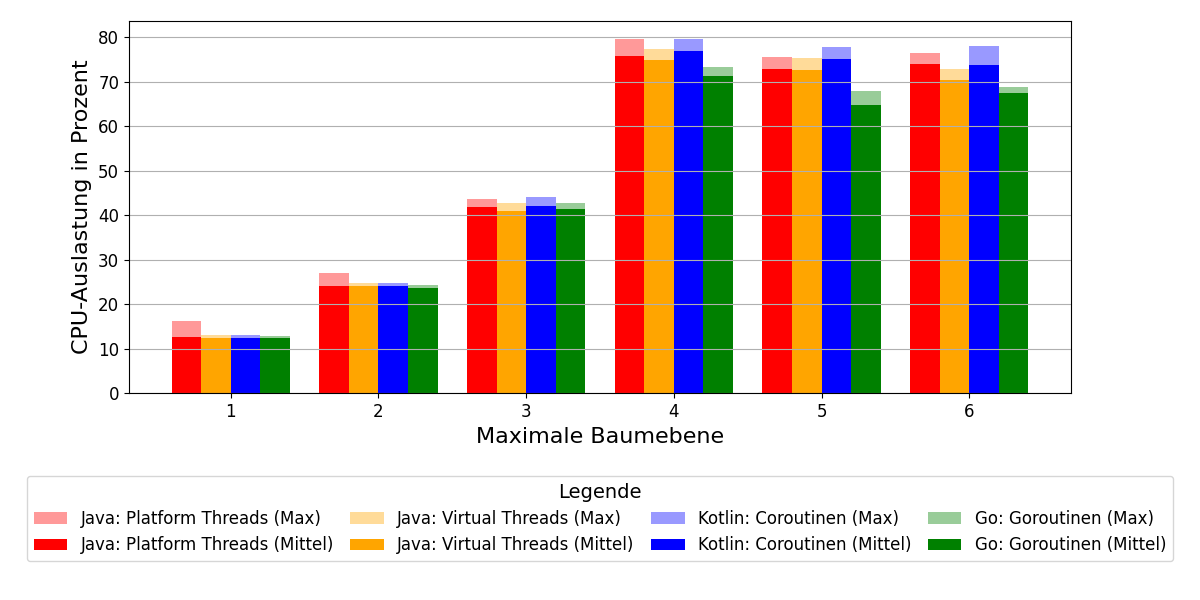
\includegraphics[scale=0.5]{figures/mergesort/Maximalebauebenen1-6/cpu_usage_bar_plot.png}
	\caption{CPU-Auslastung pro maximaler Baumebene,\\ Mergesort Messung 1: max. Baumebenen 1-6}
	\label{fig:ms1-6CPU}
\end{figure}

Die Grafik \ref{fig:ms1-6CPU} zeigt die durchschnittliche und maximale Auslastung der CPU pro maximale Baumebene. Die CPU-Auslastung wird in Prozent angegeben, wobei 100\% eine komplette Auslastung aller zur Verfügung stehenden Kerne des ausführenden Systems bedeutet.

Dabei fällt auf, dass die Werte pro maximaler Baumebene für die vier Implementierungen fast gleich sind, bei etwas geringerer Auslastung bei der Goroutinen-Implementierung. Auch die Maximalwerte für die CPU-Auslastung weichen kaum von den Mittelwerten ab. Die durchschnittliche Auslastung bei einer maximalen Baumebene 1 beträgt 12\%. Wenn der Schwellwert für die Parallelisierung bei Baumebene 1 liegt, wird der gesamte Sortier-Algorithmus auf einem Kern ausgeführt. Die Messungen wurden auf einem 8-Kern System ausgeführt, was bedeutet, dass die CPU-Auslastung bei einem ausgelasteten Kern bei 12,5\% liegt. Bei einer maximalen 
Baumebene von zwei, werden zwei Teillisten parallel sortiert. Was es den Implementierungen ermöglicht zwei Kerne auszulasten, also 25\% CPU-Auslastung. Das wird mit 24\% auch fast erreicht. Auch bei den Ergebnissen für die maximale Baumebene drei und vier wäre wieder jeweils theoretisch eine Verdoppelung zu erwarten gewesen. Dies wird jedoch nicht mehr ganz erreicht, mit einer Steigerung auf 41\% für die maximale Baumebene 3 und auf 74\% für die Ebene 4. Warum dies zu erwarten war wurde bereits in Abschnitt \ref{subsubsec:implms} erläutert. Auf Ebene fünf und sechs stagnieren die Werte, beziehungsweise gehen sogar leicht zurück, da auf Ebene vier bereits alle 8 Kerne beansprucht werden und die Parallelität nicht mehr weiter gesteigert werden kann. Der leichte Rückgang ist mit einem steigenden Overhead beim Scheduling zu erklären.

\begin{figure}[H]
	\centering
	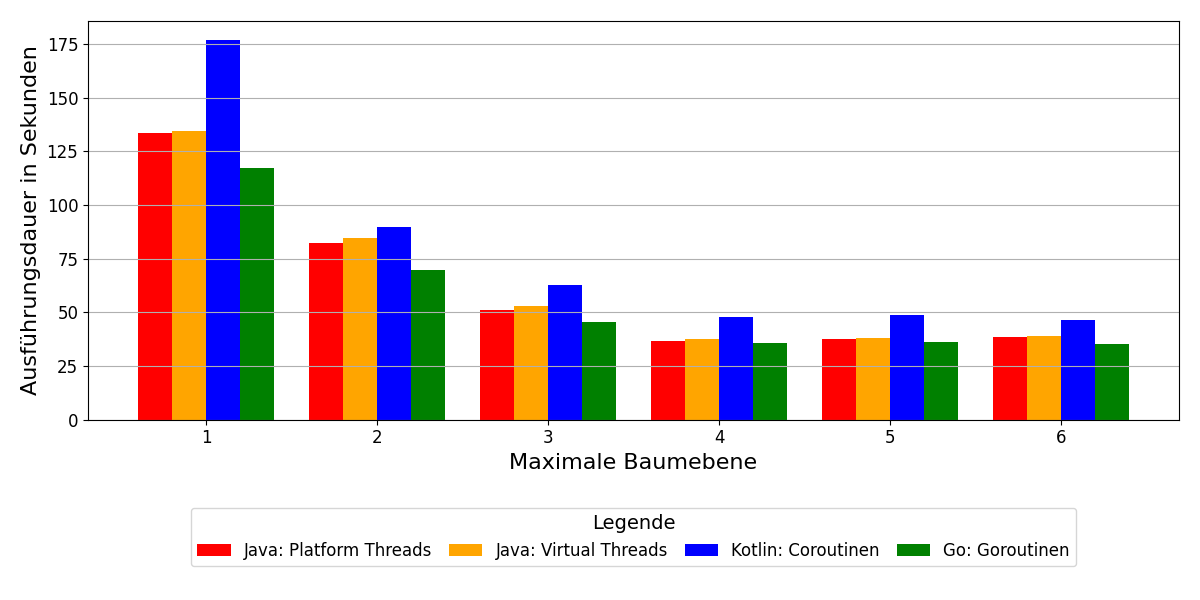
\includegraphics[scale=0.5]{figures/mergesort/Maximalebauebenen1-6/execution_time_plot.png}
	\caption{Ausführungszeit pro maximaler Baumebene,\\ Mergesort Messung 1: max. Baumebenen 1-6}
	\label{fig:ms1-6Zeit}
\end{figure}

Die Grafik \ref{fig:ms1-6Zeit} zeigt die Ausführungszeit für alle Sortierdurchläufe in Abhängigkeit von der maximalen Baumebene. Die Zeit wird in Sekunden angegeben.

Es fällt auf, dass mit steigender maximaler Baumtiefe und damit erhöhter Parallelität die Ausführungszeit abnimmt. Diese Abnahme flacht jedoch zunehmend ab, bis sie ab Baumebene 4 stagniert. Dies lässt sich durch den 8-Kern-Prozessor des ausführenden Systems erklären. Die Ausführungszeiten für Java Virtual Threads und Java Platform Threads sind nahezu identisch, mit einem leichten Vorteil für die Platform Threads. Goroutinen haben konstant eine etwas kürzere Laufzeit als die Java-Implementierungen. Coroutinen hingegen benötigen deutlich mehr Zeit.

\begin{figure}[H]
	\centering
	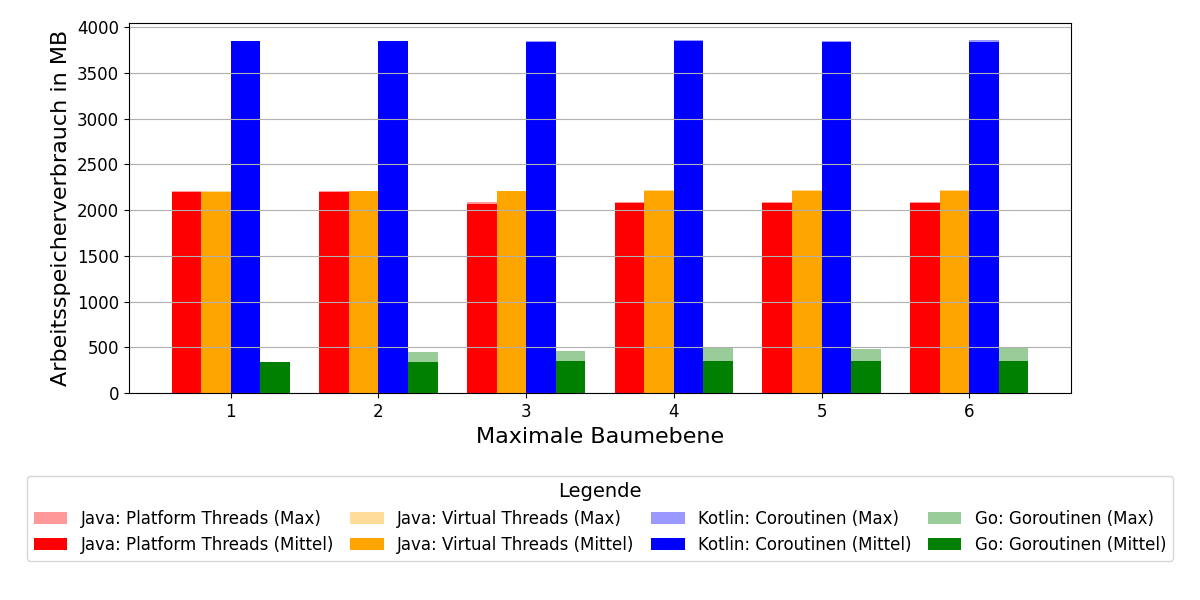
\includegraphics[scale=0.5]{figures/mergesort/Maximalebauebenen1-6/memory_usage_bar_plot.png}
	\caption{Arbeitsspeicherverbrauch pro maximaler Baumebene,\\ Mergesort Messung 1: max. Baumebenen 1-6}
	\label{fig:ms1-6RAM}
\end{figure}

Die Grafik \ref{fig:ms1-6RAM} zeigt den Arbeitsspeicherverbrauch für alle Sortierdurchläufe in Ab\-hän\-gig\-keit von der maximalen Baumtiefe. Der Arbeitsspeicherverbrauch wird in Megabyte (MB) angegeben.

Dabei ist zu beachten, dass es zwischen den maximalen und mittleren Werten kaum Unterschiede gibt, und der Verbrauch über die verschiedenen Baumebenen hinweg konstant bleibt.

Der Speicherverbrauch der Java Virtual Threads und Java Platform Threads liegt nahezu gleichauf bei etwa 2200 MB und zeigt somit fast keinen Unterschied. Hierbei ist ein leichter Vorteil für die Platform Threads zu beobachten, die einen minimal niedrigeren Speicherverbrauch aufweisen.

Im Vergleich dazu liegt der Arbeitsspeicherverbrauch der Goroutinen deutlich niedriger, bei etwa 350 MB, weist aber die größten Schwankungen zwischen den maximalen und mittel Werten auf.

Coroutinen hingegen benötigen erheblich mehr Arbeitsspeicher. Der Verbrauch liegt bei etwa  3800 MB, was eine deutlich höhere Speichernutzung im Vergleich zu den anderen Implementierungen ist.

\begin{figure}[H]
	\centering
	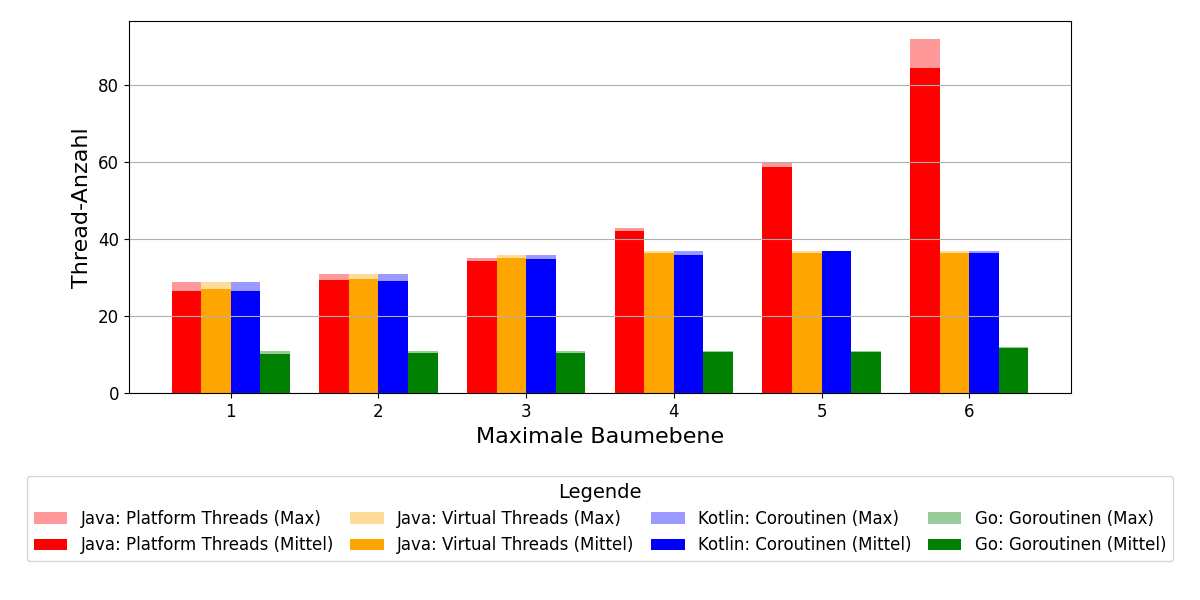
\includegraphics[scale=0.5]{figures/mergesort/Maximalebauebenen1-6/num_threads_bar_plot.png}
	\caption{Thread-Anzahl pro maximaler Baumebene,\\ Mergesort Messung 1: max. Baumebenen 1-6}
	\label{fig:ms1-6Threads}
\end{figure}

Die Grafik \ref{fig:ms1-6Threads} zeigt die Anzahl der verwendeten Betriebssystem-Threads für alle Sortierdurchläufe in Abhängigkeit von der maximalen Baumtiefe. Es werden sowohl die maximalen als auch die mittleren Thread-Anzahlen angegeben.

Es fällt auf, dass die Anzahl der verwendeten Threads, mit Ausnahme der Platform Threads, mit steigender Baumtiefe konstant bleibt oder nur moderat ansteigt. Bei Virtual Threads und Coroutinen stagnieren die verwendeten Threads ab Baumtiefe 4, bei durchschnittlich 36 Threads. Dies ist durch die Begrenzung des 8-Kern-Prozessors des Systems erklärbar. Goroutinen zeigen einen konstanten Thread-Verbrauch von durchschnittlich 10 Threads. Was mit Abstand das beste Ergebnis ist. 

Die Anzahl der verwendeten Threads bei der Implementierung mit Platform Threads zeigt mit zunehmender Baumtiefe eine exponentielle Steigerung, die in etwa den Potenzen von 2 folgt. Bei Baumtiefe 1 werden maximal 29 Threads verwendet, bei Baumtiefe 2 steigt Anzahl der maximal verwendeten Threads auf 31, bei Baumtiefe 3 auf 35 und so weiter. Die mittleren Werte liegen nur leicht darunter. Diese exponentielle Zunahme ist darauf zurückzuführen, dass für jede neue Teilliste ein neuer BS-Thread erstellt wird, was die Anzahl der verwendeten Threads mit der Baumtiefe ansteigen lässt. Die maximale Thread-Anzahl wächst also ungefähr im Muster $2^n$, wobei die Anzahl bei jeder weiteren Ebene exponentiell zunimmt.


\subsubsection{Messung 2: Mergesort - Baumebenen:1-19}

\begin{tabularx}{\textwidth}{@{}lX@{}}
	\textbf{Sortierdurchläufe:} & 100 \\
	\textbf{Listenlänge:} & 10.000.000 \\
	\textbf{Maximale Baumebene:} & \textbf{1-19} (Fokus auf 13-19) \\
	\textbf{Implementierungen:} & Java Platform Threads, Java Virtual Threads, Kotlin Coroutinen, Go Goroutinen \\
	\textbf{Aufwärmläufe:} & 10
\end{tabularx}

Im folgenden Abschnitt wird der Fokus auf die Messungen für die maximalen Baum\-ebenen 13 bis 19 gelegt. Diese spezifischen Werte werden detailliert untersucht, um die Auswirkungen der zunehmenden Baumtiefe auf die Performance der verschiedenen Implementierungen zu analysieren. Die vollständigen Messergebnisse für alle  Baumebenen von 1 bis 19 sind in Tabellenform im Anhang zu finden. Dabei werden wieder die vier Thread-Abstraktionen, Java Platform Threads, Java Virtual Threads, Kotlin Coroutinen und Go Goroutinen, verglichen. Ziel dieser Untersuchung ist es, die Skalierbarkeit und Effizienz der Implementierungen bei einem extremen Parallelisierungsgrad zu überprüfen. Allein bis einschließlich Baumebene 19 besitzt der Mergesort-Baum insgesamt 524.287 Knoten, was die immense Skalierung bei dieser Baumtiefe verdeutlicht.

Die Entscheidung, sich auf die Baumebenen 13 bis 19 zu konzentrieren, basiert auf den Ergebnissen der ersten Messung, bei der die Baumebenen 1 bis 6 detailliert untersucht wurden. Zwischen den Ebenen 4 und 13 wurden kaum Veränderungen in der Performance festgestellt, weshalb sich die Untersuchung auf die höheren Ebenen  fokussiert, um mögliche Unterschiede und Trends bei sehr großen Werten für die maximale Baumebene zu erfassen.

Die entscheidenden Performance Parameter sind dabei die Ausführungszeit pro maximaler Baumebene (Abb.: \ref{fig:ms1-19Zeit}) und Thread-Anzahl pro maximaler Baumebene (Abb.:\ref{fig:ms1-19Threads}).

\begin{figure}[H]
	\centering
	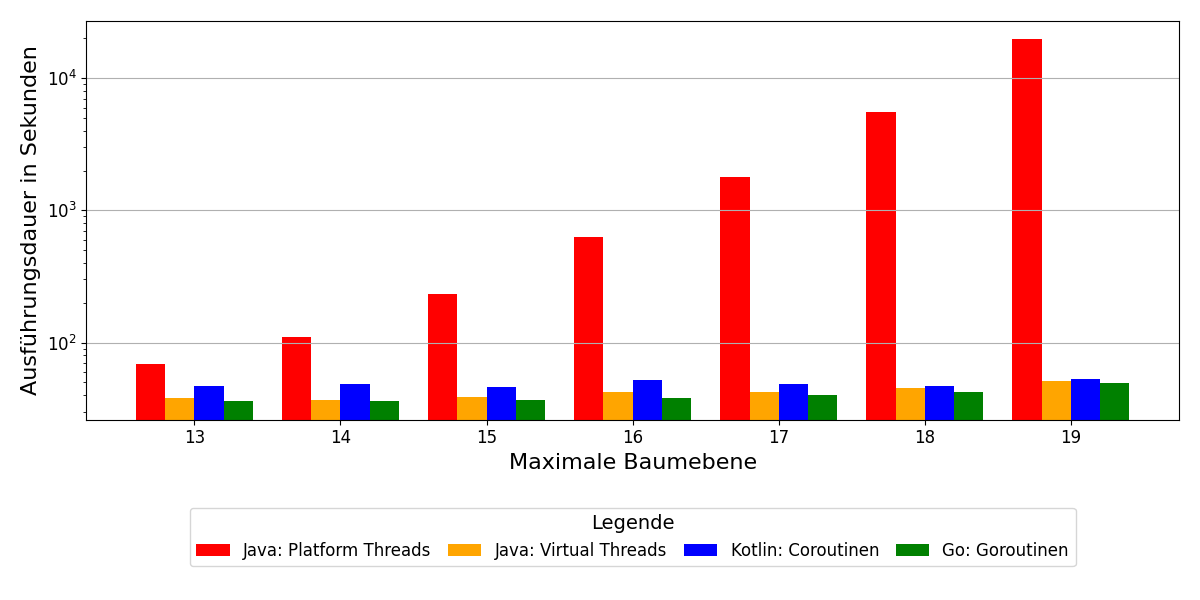
\includegraphics[scale=0.48]{figures/mergesort/Maximalebauebenen1-19_pvcg/execution_time_plot.png}
	\caption{Ausführungszeit pro maximaler Baumebene,\\ Mergesort Messung 2: max. Baumebenen 13-19}
	\label{fig:ms1-19Zeit}
\end{figure}

Die Abbildung \ref{fig:ms1-19Zeit} zeigt die Ausführungszeit pro maximaler Baumebene für die verschiedenen Thread-Abstraktionen im Bereich von 13 bis 19 Ebenen. Aufgrund der großen Unterschiede in den Ausführungszeiten wurde die y-Achse logarithmisch mit Basis 10 skaliert. Virtual Threads, Coroutinen und Goroutinen zeigen eine nahezu konstante Ausführungszeit über alle Baumebenen hinweg. Ihre Leistung bleibt stabil und ähnelt den Ergebnissen, die bereits bei der maximalen Baumebene 4 beobachtet wurden. Im Gegensatz dazu weisen Platform Threads ein exponentielles Wachstum der Ausführungszeit auf. Mit zunehmender Baumtiefe steigt die benötigte Zeit drastisch an. Die Messungen für Platform Threads wurden nach der maximalen Baumebene 19 abgebrochen, da die Ausführungszeiten für das Sortieren der Liste zu lang wurden. Diese Ergebnisse verdeutlichen die Skalierungsprobleme von Platform Threads bei extrem parallelen Aufgaben, während die anderen Thread-Abstraktionen eine bemerkenswerte Effizienz und Stabilität aufweisen.

\begin{figure}[H]
	\centering
	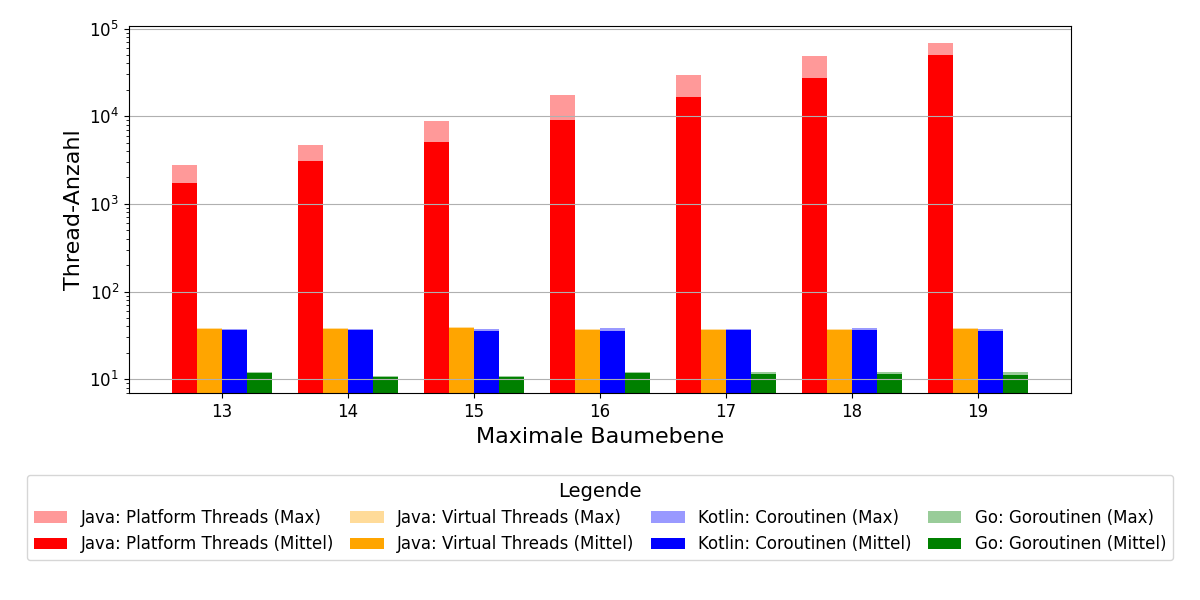
\includegraphics[scale=0.48]{figures/mergesort/Maximalebauebenen1-19_pvcg/num_threads_bar_plot.png}
	\caption{Thread-Anzahl pro maximaler Baumebene,\\ Mergesort Messung 2: max. Baumebenen 13-19}
	\label{fig:ms1-19Threads}
\end{figure}

Die Abbildung \ref{fig:ms1-19Threads} illustriert die Thread-Anzahl pro maximaler Baumebene für die verschiedenen Implementierungen. Die y-Achse ist, aufgrund der erheblichen Unterschiede in der Thread-Anzahl, ebenfalls logarithmisch mit Basis 10 skaliert. Virtual Threads, Coroutinen und Goroutinen zeigen eine konstante Thread-Anzahl über alle Baumebenen hinweg. Diese Werte entsprechen den Ergebnissen, die bereits bei der maximalen Baumebene 4 beobachtet wurden. Platform Threads hingegen weisen ein exponentielles Wachstum der Thread-Anzahl auf. Dies lässt sich dadurch erklären, dass für jeden Knoten im Baum bis zur maximalen Baumebene ein neuer Betriebssystem-Thread erstellt wird. Auf Ebene 19 werden durchschnittlich 49.881 Betriebssystem-Threads erstellt, mit einem Maximalwert von 68.210 Threads. Diese Beobachtungen führen zu zwei wichtigen Schlussfolgerungen: Erstens zeigen sich Platform Threads ineffizient bei extrem großen Thread-Zahlen und skalieren nicht mehr adäquat. Zweitens erweist sich die Implementierung trotz der enormen Thread-Anzahl als überraschend robust. Entgegen der aufgestellten Vermutungen stürzt die Anwendung nicht ab. Die Robustheit lässt sich durch die Standardkonfigurationen der verwendeten Systeme erklären: Die Java Virtual Machine (JVM) ist standardmäßig so konfiguriert, dass sie eine große Anzahl von Threads handhaben kann. Windows 11 ist ebenfalls darauf ausgelegt, mit einer hohen Anzahl von Threads umzugehen. 

Bei der CPU-Auslastung (Abb.: \ref{fig:ms1-19CPU}) lassen sich kaum Veränderungen im Vergleich zur ersten Messung feststellen und auch der Arbeitsspeicherverbrauch (Abb.: \ref{fig:ms1-19RAM}) bleibt konstant, außer für Java Platform Threads, was aber ebenfalls mit der steigenden Zahl an Threads zu erklären ist.

Diese Ergebnisse unterstreichen die Effizienz und Skalierbarkeit von Virtual Threads, Coroutinen und Goroutinen bei hochparallelen Aufgaben, während sie gleichzeitig die Grenzen von Platform Threads bei extremer Parallelisierung aufzeigen.

\subsubsection{Messung 3: Mergesort - Baumebenen:1-23}

\begin{tabularx}{\textwidth}{@{}lX@{}}
	\textbf{Sortierdurchläufe:} & 100 \\
	\textbf{Listenlänge:} & 10.000.000 \\
	\textbf{Maximale Baumebene:} & \textbf{1-23} (Fokus auf 18-23) \\
	\textbf{Implementierungen:} & \textbf{Java Virtual Threads, Kotlin Coroutinen, Go Goroutinen} (keine Java Platform Threads) \\
	\textbf{Aufwärmläufe:} & 10
\end{tabularx}

Die dritte Messung des Mergesort-Benchmarks konzentriert sich auf die extremen Bereiche der Parallelisierung, indem sie die maximalen Baumebenen von 18 bis 23 untersucht. Diese Messung zielt darauf ab, die Grenzen der Leistungsfähigkeit und Skalierbarkeit von Java Virtual Threads, Kotlin Coroutinen und Go Goroutinen unter Bedingungen extremer Parallelität zu erforschen. Java Platform Threads wurden aufgrund ihrer Limitierungen bei hoher Parallelität bewusst aus dieser Messung ausgeschlossen.

Mit bis zu 8.388.607 Knoten im Mergesort-Baum bei Ebene 23 stellt dieser Benchmark die Thread-Abstraktionen vor eine enorme Herausforderung. Die Untersuchung soll Aufschluss darüber geben, bis zu welchem Grad diese modernen Konzepte mit der zunehmenden Parallelität umgehen können und ab wann mögliche Leistungseinbrüche oder Ressourcenengpässe auftreten.

Besonders aussagekräftig sind die Ergebnisse der Ausführungszeit und der Thread-Anzahl, die in den Abbildungen \ref{fig:ms1-23Zeit} und \ref{fig:ms1-23Threads} dargestellt sind (andere Abbildungen siehe Anhang).

\begin{figure}[H]
	\centering
	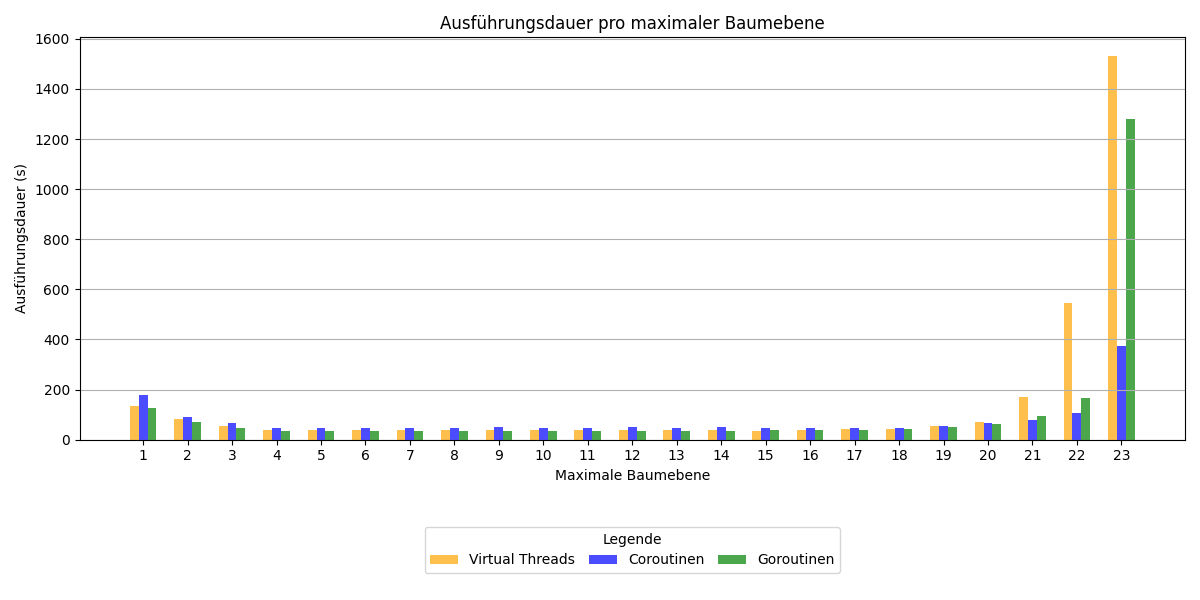
\includegraphics[scale=0.5]{figures/mergesort/Maximalebauebenen1-23_vcg/execution_time_plot.png}
	\caption{Ausführungszeit pro maximaler Baumebene,\\ Mergesort Messung 3: max. Baumebenen 18-23}
	\label{fig:ms1-23Zeit}
\end{figure}

Die Abbildung \ref{fig:ms1-23Zeit} zeigt die Ausführungszeit pro maximaler Baumebene. Dabei fällt auf, dass die Ausführungszeiten für alle drei Implementierungen lange konstant auf den Werten der maximalen Baumebene 4 bleiben. Ein Anstieg ist für Virtual Threads ab Ebene 16, für Goroutinen ab Ebene 17 und für Coroutinen ab Ebene 19 zu beobachten. Eine Verdopplung der Ausführungszeiten ist bei Ebene 20 für Virtual Threads, bei Ebene 21 für Goroutinen und bei Ebene 22 für Coroutinen festzustellen. Trotz dieser leichten Unterschiede zeigen alle Implementierungen eine ähnlich gute Performance.

\begin{figure}[H]
	\centering
	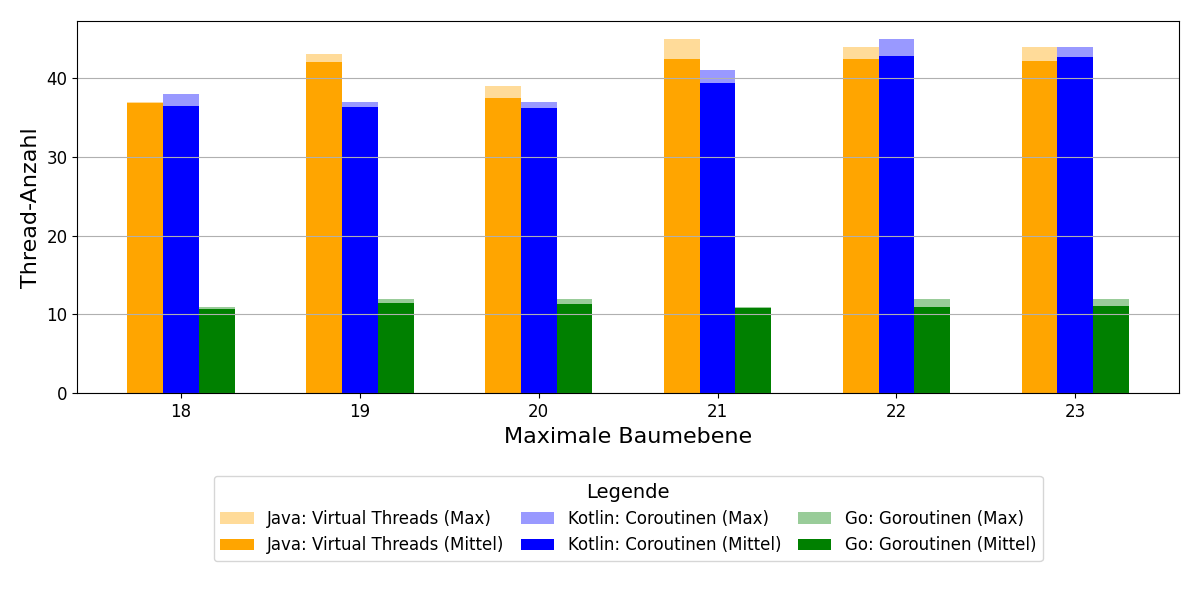
\includegraphics[scale=0.5]{figures/mergesort/Maximalebauebenen1-23_vcg/num_threads_bar_plot.png}
	\caption{Thread-Anzahl pro maximaler Baumebene,\\ Mergesort Messung 3: max. Baumebenen 18-23}
	\label{fig:ms1-23Threads}
\end{figure}

Die Abbildung \ref{fig:ms1-23Threads} stellt die Thread-Anzahl pro maximaler Baumebene dar. Bemerkenswert ist, dass die Thread-Anzahlen konstant niedrig bleiben, fast auf dem Niveau der maximalen Baumebenen. Dies deutet darauf hin, dass die Entkopplung von logischen und physischen Threads weiterhin effektiv funktioniert.

Die CPU-Auslastung, dargestellt in Abbildung \ref{fig:ms1-23CPU}, bleibt konstant hoch beziehungsweise steigt für Virtual Threads und Coroutinen sogar an. Dies lässt sich dadurch erklären, dass die Verarbeitung länger auf tieferen Baumebenen stattfindet. Lediglich Goroutinen zeigen einen leichten Abfall der CPU-Auslastung auf Ebene 22.

Der Arbeitsspeicherverbrauch, zu sehen in Abbildung \ref{fig:ms1-23RAM}, zeigt interessante Entwicklungen. Virtual Threads nähern sich im Verbrauch den Coroutinen an, während Goroutinen lange niedrig bleiben und erst ab Ebene 21 einen deutlichen Anstieg verzeichnen.

Zusammenfassend lässt sich sagen, dass alle drei Thread-Abstraktionen einen hohen Grad an Parallelität bewältigen können und in ihrer Performance dicht beieinander liegen. Die Messung gibt Aufschluss darüber, ab welchem Punkt die Effizienz nachlässt, wobei jede Implementierung leicht unterschiedliche Grenzen aufweist.

\subsubsection{Messung 4: Mergesort - Listenlänge}

\begin{tabularx}{\textwidth}{@{}lX@{}}
	\textbf{Sortierdurchläufe:} & 10000 \\
	\textbf{Listenlänge:} & \textbf{10.000 - 10.000.000} \\
	\textbf{Maximale Baumebene:} & 4 \\
	\textbf{Implementierungen:} & Java Platform Threads, Java Virtual Threads, Kotlin Coroutinen, Go Goroutinen \\
	\textbf{Aufwärmläufe:} & 10
\end{tabularx}

Die vierte Messung des Mergesort-Benchmarks konzentriert sich auf den Einfluss der Listenlänge auf die Performance-Unterschiede zwischen den verschiedenen Thread-Abs\-trak\-ti\-onen. Für diese Untersuchung wurden Listenlängen von 10.000 bis 10.000.000 Elementen getestet, wobei die maximale Baumebene konstant bei 4 gehalten wurde. So können alle 8 Kerne des Prozessors genutzt werden.

Das Hauptziel dieser Messung war es, festzustellen, ob die Listenlänge einen signifikanten Einfluss auf die relativen Leistungsunterschiede zwischen den verschiedenen Thread-Abstraktionen hat. Die Ergebnisse zeigten jedoch, dass alle getesteten Implementierungen gleichermaßen mit der Listenlänge skalierten. Die beobachteten Performance-Unterschiede zwischen den Thread-Abstraktionen blieben über den gesamten Bereich der getesteten Listenlängen weitgehend konstant.

Aufgrund dieser Beobachtung und da keine neuen Erkenntnisse gewonnen wurden, die über die vorherigen Messungen hinausgingen, wurden die detaillierten Ergebnisse dieser Messung in den Anhang verschoben. Für tiefergehende Analysen können die entsprechenden Graphen im Abschnitt \ref{subsec:mergsort4graph} und die zugehörigen Tabellen im Abschnitt \ref{subsec:mergsort4tabellen} eingesehen werden.

\subsubsection{Fazit: Mergesort}

Der Mergesort-Benchmark erwies sich letztendlich als ein rechenintensiver Benchmark, bei dem der Grad der Parallelisierung durch die Anpassung der maximalen Baumebenen gesteuert werden konnte. Bei niedrigen Baumebenen zeigten alle vier Thread-Abstraktionen eine vergleichbare Skalierung hinsichtlich der CPU-Auslastung. Infolgedessen konnten Virtual Threads, Coroutinen und Goroutinen keine signifikant besseren Ergebnisse bei der Ausführungszeit erzielen als Platform Threads. Interessanterweise benötigten Coroutinen sogar die längste Ausführungszeit.

Bezüglich des Arbeitsspeicherverbrauchs lagen Virtual Threads und Platform Threads gleichauf, während Coroutinen den mit Abstand höchsten Verbrauch aufwiesen. Goroutinen hingegen zeichneten sich durch den deutlich geringsten Arbeitsspeicherverbrauch aus.

Die Anzahl der Threads offenbarte den markantesten Unterschied zwischen den neuen Technologien und Platform Threads. Während die Anzahl der Threads bei den neuen Technologien konstant niedrig blieb, stieg sie bei Platform Threads mit zunehmenden maximalen Baumebenen und damit steigender Parallelisierung kontinuierlich an. Dieser Anstieg führte zu einer Verlangsamung der Ausführung.

Die neuen Technologien konnten aufgrund ihrer Entkoppelung von BS-Threads eine deutlich größere Zahl an Threads handhaben. Performanceeinbrüche traten bei ihnen erst bei einem  hohen Grad an Parallelisierung auf, jedoch deutlich später als bei Platform Threads.

\newpage

\section{Benchmark 2: Bank}

\subsection{Motivation: Bank}

Um die Leistungsfähigkeit und Praxistauglichkeit der verschiedenen Thread-Abs\-trak\-tio\-nen in einem realitätsnahen Szenario zu untersuchen, wurde im Rahmen der Masterarbeit ein Bankensystem-Bench\-mark entwickelt. Dieser Benchmark simuliert eine rudimentäre Bank, die nicht den Anspruch erhebt die Komplexität eines realen Bankensystems abzubilden, sondern vielmehr als anschauliches Beispiel für nebenläufige Operationen in einer typischen Ge\-schäfts\-an\-wen\-dung dient.

Das simulierte Bankensystem verwaltet Konten und führt Überweisungen zwischen diesen Konten durch. Bei jeder Überweisung wird ein Betrag von einem Konto abgebucht und einem anderen gutgeschrieben, wobei die Konsistenz des Datensatzes zu jedem Zeitpunkt gewährleistet sein muss. Diese Anforderung stellt eine klassische Herausforderung für nebenläufige Systeme dar, da gleichzeitige Zugriffe auf dieselben Konten koordiniert werden müssen, um Race Conditions und inkonsistente Zustände zu vermeiden.

Ein wesentlicher Aspekt dieses Benchmarks ist die Integration verschiedener Technologien, die in modernen Softwarearchitekturen häufig zum Einsatz kommen:

\begin{itemize}
	\item \textbf{PostgreSQL:} Als robuste, relationale Datenbank zur Speicherung der Kontoinformationen.
	\item \textbf{PostgREST:} Ein RESTful API-Server für PostgreSQL, der eine zusätzliche Abstraktionsebene zwischen Anwendung und Datenbank bietet.
	\item \textbf{Docker:} Zur Containerisierung und einfachen Bereitstellung der einzelnen Komponenten sowie zur Zuweisung von Hardwareressourcen.
	\item \textbf{Datenbanktreiber / Datenbankverbindungspools:} Zur effizienten Verwaltung von Datenbankverbindungen.
\end{itemize}

Die Verwendung dieser Technologien stellt sicher, dass die Thread-Abs\-trak\-tio\-nen in einer Umgebung getestet werden, die typischen Produktivsystemen ähnelt. Insbesondere die Interaktion mit der Datenbank repräsentiert eine blockierende I/O-Operation, wie sie in vielen realen Anwendungen vorkommt.

Durch diesen Aufbau kann nicht nur die reine Leistungsfähigkeit der Thread-Abs\-trak\-tio\-nen gemessen werden, sondern auch ihre Fähigkeit zur effektiven Zusammenarbeit mit externen Systemen und zur Handhabung von I/O-gebundenen Aufgaben evaluiert werden. Dies ermöglicht eine umfassendere Beurteilung ihrer Praxistauglichkeit und Effizienz in komplexen, verteilten Systemen.

Der Bank-Benchmark wird somit zu einem aussagekräftigen Indikator für die Leis\-tungs\-fä\-hig\-keit und Skalierbarkeit der verschiedenen Thread-Abstraktionen in einem Szenario, das typische Herausforderungen moderner Softwarearchitekturen widerspiegelt.

\subsection{Implementierung: Bank}

\subsubsection{Basisimplementierung: Bank}

\paragraph{Testdatengenerierung:}
\label{para:datagenerator}

 Vor dem Ausführen des Benchmarks müssen zuerst die Testdaten generiert werden. Konkret sind dies einerseits die Bankkonten (Accounts), welche sich aus einer Kontonummer und einem Kontostand zusammen setzen, andererseits die Überweisungen (Transactions) welche aus einem Sender, einem Empfänger und dem zu überweisenden Betrag bestehen. Dieses Daten werden von der separaten Anwendung \texttt{bankDataGenerator.jar} generiert. Diese erhält zwei Übergabeparameter: die Anzahl der Konten und die Anzahl der Überweisungen. Auf dieser Grundlage werden zwei Textdateien erstellt, welche dann von den unterschiedlichen Implementierungen importiert werden können, sodass gewährleistet ist, dass alle mit den gleichen Daten arbeiten. Das Ausführen von \texttt{bankDataGenerator.jar} findet zu Beginn des Python-Scripts \texttt{monitoring""Bank.py} (Abschnitt: \ref{subsubsec:monibank}) statt.
 
\paragraph{PostgreSQL:}

PostgreSQL dient als robuste, relationale Datenbank zur Speicherung der Kontodaten. Die Kontoinformationen werden in einer Tabelle mit zwei Spalten gespeichert: Kontonummer (accountId) und Kontostand (balance). Ein zentrales Ziel des Benchmarks ist es, die Datenkonsistenz zu wahren, weshalb jede Überweisung als Transaktion behandelt wird.

PostgreSQL bietet ein leistungsfähiges Transaktionskonzept, das die ACID-Eigenschaften (Atomicity, Consistency, Isolation, Durability) gewährleistet. Eine Transaktion in PostgreSQL ist eine Sequenz von Datenbankoperationen, die als eine einzige, unteilbare Einheit behandelt wird. Sie beginnt mit dem Befehl BEGIN und endet entweder mit COMMIT, um die Änderungen zu speichern, oder mit ROLLBACK, um sie rückgängig zu machen.

Für die Verwaltung konkurrierender Zugriffe verwendet PostgreSQL Zeilensperren. Wenn eine Transaktion bereits Sperren auf den betroffenen Konten hält, wartet eine konkurrierende Transaktion, bis diese Sperren freigegeben werden. Dies stellt sicher, dass keine inkonsistenten Zustände entstehen.

PostgreSQL verfügt über eine integrierte Deadlock-Erkennung. Wenn zwei Transaktionen gegenseitig aufeinander warten, erkennt PostgreSQL den Deadlock und bricht eine der Transaktionen ab, um die Blockade aufzulösen.
Um die Häufigkeit von Deadlocks zu reduzieren, wird eine Strategie implementiert, bei der bei Überweisungen immer zuerst das Konto mit der kleineren Kontonummer gesperrt wird. Dies gewährleistet eine konsistente Reihenfolge beim Sperren von Ressourcen und minimiert das Risiko von Deadlocks.

Durch die Verwendung von PostgreSQL als Datenbank für den Bank-Benchmark wird eine realitätsnahe Umgebung geschaffen, die typische Herausforderungen in Bezug auf Datenkonsistenz und Nebenläufigkeit in Geschäftsanwendungen widerspiegelt. Dies er\-mög\-licht eine aussagekräftige Evaluation der verschiedenen Thread-Abstraktionen in einem praxisnahen Szenario.

\paragraph{PostREST:}

PostgREST ist ein leistungsfähiges Open-Source-Tool, das automatisch eine RESTful-API für PostgreSQL-Datenbanken generiert. Es erstellt dynamisch Endpunkte für Tabellen und Views in der Datenbank, wodurch eine schnelle und flexible Schnittstelle zwischen der Datenbank und den Anwendungen geschaffen wird.

Ein wesentlicher Vorteil von PostgREST ist, dass es PostgreSQL-Funktionen als Remote Procedure Calls (RPC) verfügbar macht. Für den Bank-Benchmark wurden entsprechende Funktionen in der Datei \texttt{init.sql} definiert und in der Datenbank gespeichert. Diese Funktionen sind:

\begin{itemize}
	\item \texttt{create\_account}: Zum Erstellen neuer Bankkonten
	\item \texttt{delete\_all\_accounts}: Zum Löschen aller Konten (nützlich für das Zurücksetzen des Benchmarks)
	\item \texttt{transfer\_balance}: Zur Durchführung von Überweisungen zwischen Konten
\end{itemize}

Die Verwendung von PostgREST als Schnittstelle wurde mit dem Ziel gewählt, eine faire Vergleichsbasis für alle Implementierungen zu schaffen. Durch die einheitliche REST-Schnitt\-stel\-le wird sichergestellt, dass alle Thread-Abstraktionen unter gleichen Bedingungen auf die Datenbank zugreifen. Ein weiterer Vorteil ist, dass keine spezifischen Datenbanktreiber für die verschiedenen Programmiersprachen benötigt werden, was die Implementierung vereinfacht und mögliche Unterschiede in der Leistungsfähigkeit der Treiber ausschließt.

In der praktischen Durchführung des Benchmarks hat sich jedoch gezeigt, dass PostgREST zum limitierenden Faktor bei der Skalierung wurde und letztendlich in diesem Aufbau eine ähnliche Funktion wie ein Datenbankverbindungspool übernehmen würde. Deshalb ist PostgREST kein Teil der finalen Messungen für diesen Benchmark.

\paragraph{Docker:}
\label{para:docker}

Docker spielt eine zentrale Rolle in der Implementierung des Bank-Bench\-marks, indem es ermöglicht, alle Komponenten in isolierten Containern laufen zu lassen. Diese Containerisierung ist heutzutage typisch für moderne Softwarearchitekturen und bietet mehrere Vorteile für den Benchmark-Aufbau.

\begin{itemize}
	\item Konsistenz: Alle Tests laufen in der gleichen, reproduzierbaren Umgebung.
	\item Isolation: Jede Komponente läuft in ihrem eigenen Container, was Interferenzen minimiert.
	\item Portabilität: Der gesamte Benchmark-Stack kann leicht auf verschiedenen Systemen ausgeführt werden.
\end{itemize}

Die Hauptkomponenten des Benchmarks, die in Docker-Containern laufen, sind:

\begin{itemize}
	\item Benchmark-Implementierungen: bank-java, bank-go, bank-kotlin
	\item PostgreSQL-Datenbank
	\item PostgREST (in der finalen Version nicht mehr verwendet)
\end{itemize}

Der gesamte Benchmark-Stack wird über eine \texttt{docker-compose.yaml} Datei orchestriert und gestartet. Diese Konfiguration ermöglicht es, die gesamte Benchmark-Umgebung mit einem einzigen Befehl zu starten und zu verwalten.
Ein wichtiger Aspekt des Setups ist das Python-Skript \texttt{monitoringBank.py}, welches die Möglichkeit bietet die docker-compose-Datei zu modifiziern, um Umgebungsvariablen zu setzen und Messparameter zu verändern. Dies erlaubt es, verschiedene Szenarien für den Benchmark zu konfigurieren und zu testen. Eine detaillierte Auflistung der verfügbaren Messparameter findet sich im Abschnitt \ref{subsec:parabank}.

Um sicherzustellen, dass die Benchmark-Implementierungen erst starten, wenn die Post\-greSQL-Datenbank vollständig initialisiert und betriebsbereit ist, wurde ein Healthcheck für den PostgreSQL-Container implementiert. Dies verhindert Fehlstarts und ge\-währ\-leis\-tet konsistente Testbedingungen.

Ein entscheidender Aspekt des Docker-Setups ist die Zuweisung fester Hardwareressourcen (CPU und RAM) zu den einzelnen Containern. Dies wird über die \texttt{resources}-Konfiguration in der Docker-Compose-Datei realisiert. Durch diese Ressourcenbegrenzung wird simuliert, dass die verschiedenen Komponenten auf getrennten Systemen laufen, was die Realitätsnähe des Benchmarks erhöht und eine fairere Vergleichsbasis für die verschiedenen Implementierungen schafft.

Durch diesen Aufbau wird eine realitätsnahe und gut kontrollierbare Umgebung für den Vergleich der verschiedenen Thread-Abstraktionen geschaffen, die moderne Softwarearchitekturen widerspiegelt und gleichzeitig eine hohe Reproduzierbarkeit der Ergebnisse gewährleistet.

\paragraph{Allgemeingültige Implementierungsdetails:}

Um eine effiziente und vergleichbare Aus\-füh\-rung zu gewährleisten, wurden bei der Implementierung des Bank-Bench\-marks  mehrere allgemeingültige Designentscheidungen getroffen:

Zunächst wurde das Interface BankAccountRepository implementiert. Dieses ermöglicht sowohl Implementierungen für Datenbanktreiber als auch für REST-Schnittstellen, was die Vergleichbarkeit zwischen verschiedenen Ansätzen erhöht und eine flexible Architektur schafft.

Der implementierte Code enthält zudem einen Retry-Mechanismus, der hauptsächlich für die PostgREST-Implementierung konzipiert wurde. Obwohl dieser Mechanismus auch in die direkte Datenbankimplementierung integriert wurde, erwies er sich während der Testdurchläufe dort als nicht notwendig. Die Integration dieses Mechanismus in beide Implementierungen dient der Vergleichbarkeit der Ergebnisse und gewährleistet eine konsistente Fehlerbehandlung über verschiedene Szenarien hinweg.

Durch die Verwendung eines gemeinsamen Interfaces und die Integration verschiedener Ansätze lässt sich der Benchmark in Zukunft leicht um weitere Lösungen erweitern, was eine kontinuierliche Evaluation neuer Technologien und Methoden ermöglicht.


\subsubsection{Platform Threads: Bank}

Die Implementierung der Bank-Anwendung mit Java Platform Threads erfolgt in der Anwendung \texttt{bankJava.jar}, die in einem Docker Container namens \texttt{bank-java} ausgeführt wird.

Die Klasse \texttt{JDBCBankAccountRepository} implementiert das Interface \texttt{Bank""Account""Re""po""si""to""ry} und stellt die Datenbankzugriffe bereit. Für die Datenbankverbindung wird JDBC in Verbindung mit dem PostgreSQL-Treiber (Version 42.7.2) verwendet. 

Zur effizienten Verwaltung der Datenbankverbindungen kommt HikariCP (Version 6.0.0) zum Einsatz, ein leistungsstarker Connection Pool. HikariCP wurde aufgrund seiner hervorragenden Performance und seines geringen Overheads ausgewählt. Außerdem ist es eine weitverbreitete Technologie, die so dem Anspruch auf Realitätsnähe gerecht wird.

Die Auswahl der spezifischen Implementierung wird über die Klasse \texttt{Transaction""Exe""cu""tor} gesteuert. Für die Ausführung mit Platform Threads ist die Methode \texttt{execute""Trans""ac""ti""ons""Platform} zuständig. Diese Methode nutzt einen Fixed Thread Pool, der mit \texttt{Executors"".new""Fixed""Thread""Pool""(maxConnections*2)} initialisiert wird. Es werden also doppelt so viele Platform Threads wie Datenbankverbindungen erstellt. Dadurch ist gewährleistet, dass theoretisch alle Datenbankverbindungen aus dem Connection Pool genutzt werden können. Die Anzahl der Threads bleibt dennoch überschaubar, sodass die Systemressourcen nicht übermäßig belastet werden.


\subsubsection{Virtual Threads: Bank}

Die Implementierung der Bank-Anwendung mit Java Virtual Threads erfolgt ebenfalls in der Anwendung \texttt{bankJava.jar}, die im gleichen Docker Container \texttt{bank-java} ausgeführt wird wie die Platform Threads Variante.

Auch hier kommt die Klasse \texttt{JDBCBankAccountRepository} zum Einsatz, die das Interface \texttt{BankAccountRepository} implementiert. Die Datenbankzugriffe werden weiterhin über JDBC mit dem PostgreSQL-Treiber (Version 42.7.2) realisiert. Die Verwendung von JDBC ermöglicht eine konsistente Implementierung zwischen Java Platform Threads und Virtual Threads, was den Vergleich der Leistung erleichtert. Es ist anzumerken, dass die Unterstützung für Virtual Threads in JDBC-Treibern noch relativ neu ist und stetig verbessert wird.

Für das Verbindungs-Pooling wird ebenfalls HikariCP (Version 6.0.0) verwendet. HikariCP hat in neueren Versionen Optimierungen für die Arbeit mit Virtual Threads eingeführt, um deren Vorteile optimal zu nutzen. Die Beibehaltung von HikariCP für Virtual Threads ermöglicht eine faire Vergleichsbasis und nutzt gleichzeitig die spezifischen Optimierungen für diese neue Technologie.

Die Auswahl der spezifischen Implementierung wird, wie bei den Platform Threads, über die Klasse \texttt{TransactionExecutor} gesteuert. Für die Ausführung mit Virtual Threads ist die Methode \texttt{executeTransactionsVirtual} zuständig.
Im Gegensatz zur Platform Threads Implementierung wird hier \texttt{Executors.newVirtualThreadPerTaskExecutor()} verwendet. Dieser Executor erstellt für jede Aufgabe einen neuen Virtual Thread.

Um die Anzahl der gleichzeitigen Datenbankzugriffe zu begrenzen, wird eine Semaphore mit \texttt{maxConnections*2} Genehmigungen verwendet. Dies entspricht der Anzahl der Threads im Fixed Thread Pool der Platform Threads Implementierung, gewährleistet aber eine flexiblere Handhabung der Nebenläufigkeit. In der Praxis hat sich gezeigt, dass HikariCP zwar auch deutlich mehr gleichzeitige Anfragen von Virtual Threads verarbeiten kann (zehntausende), aber der Overhead für die Verwaltung steigt und es deshalb sinnvoll ist, die gleichzeitigen Anfragen an den Pool zu limitieren.

Der Hauptunterschied zwischen den beiden Implementierungen liegt also in der Art, wie auf den Connection Pool zugegriffen wird: Bei Platform Threads geschieht dies über einen festen Thread Pool, während bei Virtual Threads für jede Aufgabe ein neuer Thread erstellt wird, der aber durch die Semaphore in seiner Zugriffshäufigkeit auf den Pool begrenzt wird.

\subsubsection{Coroutinen: Bank}

Die Implementierung der Bank-Anwendung mit Kotlin Coroutinen erfolgt in der Anwendung \texttt{bankKotlinFat.jar}, die in einem Docker Container namens \texttt{bank-kotlin} ausgeführt wird.

Die Klasse \texttt{R2DBCBankAccountRepository} implementiert das Interface \texttt{Bank""Account""Repo""si""tory} und stellt die Datenbankzugriffe bereit. Für die Datenbankverbindung wird der R2DBC-Treiber (Version 1.0.7.RELEASE) in Verbindung mit einem Connection Pool (Version 1.0.0.RELEASE) verwendet. 

Die Wahl fiel auf R2DBC, da es eine der wenigen Kombinationen aus Datenbankteiber und Connection Pool ist, die native Unterstützung für Coroutinen bietet. Allerdings wird dabei ein reaktiver Ansatz verfolgt.

Zur Unterstützung der reaktiven Programmierung mit Coroutinen wird die Bibliothek \texttt{kot""linx-""coroutines-""reactive} verwendet. Diese ermöglicht eine nahtlose Integration zwischen reaktiven Streams und Coroutinen, was die Verarbeitung asynchroner Datenbankoperationen erheblich vereinfacht.

Die Ausführung der Transaktionen wird über die Klasse \texttt{TransactionExecutor} und speziell die Methode \texttt{executeTransactionsCoroutine} gesteuert. Ein bemerkenswerter Aspekt dieser Implementierung ist, dass die Zugriffe auf den Connection Pool nicht limitiert wurden. Diese Entscheidung basiert auf praktischen Erfahrungen, die gezeigt haben, dass dieser Ansatz in Verbindung mit Coroutinen die besten Ergebnisse liefert.

Für die Ausführung der Datenbankoperationen wurde der \texttt{Dispatchers.IO} verwendet. Dieser Dispatcher ist speziell für I/O-intensive Aufgaben wie Datenbankzugriffe optimiert.

Durch den Einsatz von R2DBC in Verbindung mit Coroutinen wird eine reaktive und nicht-blockierende Verarbeitung der Datenbankoperationen erreicht. Dies führt zu einer verbesserten Ressourcennutzung und potenziell höherem Durchsatz, insbesondere bei einer großen Anzahl gleichzeitiger Anfragen.

\subsubsection{Goroutinen: Bank}

Die Implementierung der Bank-Anwendung mit Go Goroutinen erfolgt in der Anwendung \texttt{bankGo.exe} (für Windows) beziehungsweise \texttt{bankGo} (für Unix-basierte Systeme), die in einem Docker Container namens \texttt{bank-go} ausgeführt wird.

Die Datei \texttt{SQLBankAccountRepository.go} implementiert das Interface \texttt{Bank""Account""Repo""sitory"".go} und stellt die Datenbankzugriffe bereit. Für die Datenbankverbindung wird der Treiber pgx (Version 5.7.1) verwendet. Pgx ist ein leistungsstarker Postgre\-SQL-Treiber und -Toolkit für Go, der mehrere Vorteile bietet:

\begin{itemize}
	\item Integrierte Verbindungspooling-Funktionalität
	\item Automatische Nutzung des Go-eigenen Net Pollers für effiziente Netzwerk-I/O
	\item Optimierte Performance durch effiziente Protokollimplementierung
\end{itemize}

Die Verwendung des Net Pollers ermöglicht es, eine große Anzahl von Datenbankverbindungen effizient zu verwalten, ohne für jede Verbindung einen separaten Betriebssystem-Thread zu blockieren.

Die Steuerung der Überweisungen erfolgt in der Datei \texttt{TransactionExecutor.go} durch die Funktion \texttt{executeTransactionsGoroutine}. Diese Funktion nutzt Goroutinen, um die Überweisungen parallel auszuführen.

Um die Anzahl der gleichzeitigen Datenbankzugriffe zu begrenzen, wird ein Semaphore mit \texttt{maxConnections*2} Genehmigungen verwendet. Dies entspricht der Anzahl der Threads im Fixed Thread Pool der Java Platform Threads Implementierung und der Semaphore-Größe in der Virtual Threads Implementierung. Es ist durchaus möglich mehr Anfragen gleichzeitig an den Pool zu senden, jedoch führt dies zu einer leicht erhöhten Ausführungszeit und deutlich erhöhtem Arbeitsspeicherverbrauch.

Die Verwendung von Goroutinen in Kombination mit dem effizienten pgx-Treiber und dem integrierten Scheduler von Go ermöglicht eine hochgradig skalierbare und effiziente Verarbeitung von Datenbankoperationen.

\subsection{Messparameter: Bank}
\label{subsec:parabank}

Für den Bank-Benchmark können verschiedene Parameter variiert werden, um die Leistungsfähigkeit der unterschiedlichen Thread-Abstraktionen zu testen. Die Parameter werden in der \texttt{docker-compose\_modify.yaml} Datei festgelegt und können von dem Python-Skript \texttt{monitoringBank.py} verändert werden. Im Folgenden werden die wichtigsten Messparameter vorgestellt, die für die Durchführung und Auswertung des Benchmarks von Bedeutung sind.

\subsubsection{Implementierungen}

Der Parameter gibt an, welche Thread-Abstraktion für die Implementierung des Benchmarks verwendet wird. Diese Auswahl bestimmt maßgeblich, wie die nebenläufigen Operationen im Benchmark ausgeführt werden. Jede Thread-Abstraktion hat ihre eigenen Charakteristiken und Optimierungen, was einen direkten Einfluss auf die Performance und das Verhalten des Benchmarks hat.

\begin{tabularx}{\textwidth}{@{}lX@{}}
	\textbf{Parameter:} & \texttt{ALGORITHM} \\
	\textbf{Beschreibung:} & Legt die zu verwendende Thread-Abstraktion für den Benchmark fest. \\
	\textbf{Typischer Wert:} & \texttt{PLATFORM, VIRTUAL, COROUTINE, GOROUTINE}
\end{tabularx}

\subsubsection{Datenbankschnittstelle}

Der Parameter gibt an, welche Datenbankschnittstelle für die Implementierung des Benchmarks verwendet wird. Diese Auswahl bestimmt, wie die Datenbankoperationen im Benchmark ausgeführt werden.

\begin{tabularx}{\textwidth}{@{}lX@{}}
	\textbf{Parameter:} & \texttt{INTERFACE\_TYPE} \\
	\textbf{Beschreibung:} & Legt die zu verwendende Datenbankschnittstelle für den Benchmark fest. \\
	\textbf{Typischer Wert:} & \texttt{PGX, JDBC, R2DBC, REST}
\end{tabularx}

\subsubsection{Anzahl der Bankkonten}

Der Parameter gibt die Gesamtzahl der Bankkonten an, die für den Benchmark verwendet werden. Diese Zahl beeinflusst die Komplexität und den Umfang der Simulation. Ein Bankkonto besteht immer aus einer Kontonummer und einem Kontostand.

\begin{tabularx}{\textwidth}{@{}lX@{}}
	\textbf{Parameter:} & \texttt{NUMBER\_OF\_ACCOUNTS} \\
	\textbf{Beschreibung:} & Legt die Anzahl der Bankkonten fest, die im Benchmark simuliert werden. \\
	\textbf{Typischer Wert:} & 1000 (Eintausend Bankkonten)
\end{tabularx}

\subsubsection{Anzahl der Überweisungen}

Der Parameter gibt die Gesamtzahl der Überweisungen an, die während des Benchmarks durchgeführt werden sollen. Diese Zahl beeinflusst die Laufzeit und den Umfang des Tests sowie die Menge der zu verarbeitenden Daten. Eine höhere Anzahl von Überweisungen erhöht die statistische Zuverlässigkeit der Testergebnisse, da zufällige Schwankungen ausgeglichen werden. Gleichzeitig steigt mit der Anzahl der Transaktionen auch die Gesamtlaufzeit des Benchmarks. Eine Überweisung besteht immer aus einem Sender, einem Empfänger und dem zu überweisenden Betrag. 

\begin{tabularx}{\textwidth}{@{}lX@{}}
	\textbf{Parameter:} & \texttt{NUMBER\_OF\_TRANSACTIONS} \\
	\textbf{Beschreibung:} & Legt die Anzahl der Überweisungen fest, die im Benchmark durchgeführt werden. \\
	\textbf{Typischer Wert:} & 100.000 (Einhunderttausend Transaktionen)
\end{tabularx}

\subsubsection{Maximale Datenbankverbindungen}

Der Parameter gibt die maximale Anzahl gleichzeitiger Datenbankverbindungen an, die der Verbindungspool verwalten kann. Diese Begrenzung beeinflusst direkt die Skalierbarkeit und Ressourcennutzung des Systems.

\begin{tabularx}{\textwidth}{@{}lX@{}}
	\textbf{Parameter:} & \texttt{MAX\_CONNECTIONS} \\
	\textbf{Beschreibung:} & Legt die maximale Anzahl gleichzeitiger Datenbankverbindungen fest. \\
	\textbf{Typischer Wert:} & 80 (Achtzig Verbindungen)
\end{tabularx}

\subsubsection{Verzögerung der Überweisungen}

Der Parameter gibt an, ob und wie lange eine künstliche Verzögerung (in Sekunden) für jede Transaktion in der Datenbank eingefügt werden soll. Diese Verzögerung wird direkt in der PostgreSQL-Datenbank mittels der \texttt{pg\_sleep}-Funktion implementiert. Dieser Parameter erlaubt es, die Leistungsfähigkeit der verschiedenen Thread-Abstraktionen unter unterschiedlicher Latenz der Datenbank zu vergleichen, ohne die Anwendungslogik selbst zu verändern.

\begin{tabularx}{\textwidth}{@{}lX@{}}
	\textbf{Parameter:} & \texttt{DELAY\_TRANSACTION} \\
	\textbf{Beschreibung:} & Legt die Dauer der künstlichen Verzögerung für jede Transaktion in Sekunden fest. \\
	\textbf{Typischer Wert:} & 0.0 (Keine künstliche Verzögerung)
\end{tabularx}

\subsubsection{Ressourcenbeschränkungen}
\label{subsubsec:bankRes}

Für die Durchführung des Bank-Benchmarks wurden spezifische Ressourcenbe\-schrän\-kun\-gen für die Docker-Container festgelegt. Diese Einschränkungen dienen dazu, eine konsistente und kontrollierte Testumgebung zu gewährleisten und die Vergleichbarkeit der Ergebnisse zwischen verschiedenen Implementierungen sicherzustellen.

Für den Postgres-Datenbankcontainer wurden folgende Ressourcenlimits definiert:
\begin{itemize}
	\item \textbf{CPU-Reservierung/Limit}: 3 CPUs
\end{itemize}

Für den Bank-Benchmark-Container wurden folgende Ressourcenbeschränkungen festgelegt:
\begin{itemize}
	\item \textbf{CPU-Reservierung/Limit}: 4 CPUs
	\item \textbf{Arbeitsspeicher-Reservierung/Limit}: 4000 MB
\end{itemize}

\subsection{Messungen: Bank}

Der Abschnitt präsentiert die Messergebnisse des Bank-Benchmarks. Die Resultate werden in Form von Graphen dargestellt, während die konkreten Messwerte in Tabellen im Anhang zu finden sind.

Bei allen durchgeführten Messungen kamen Datenbanktreiber und Verbindungs-Pools zum Einsatz. Da diese Komponenten durchgängig verwendet wurden, wird dies nicht bei jeder einzelnen Messung explizit erwähnt.

Die Ressourcenbeschränkungen, die in Abschnitt \ref{subsubsec:bankRes} definiert wurden, blieben für alle Messungen unverändert. Dies gewährleistet eine konsistente Testumgebung und ermöglicht einen aussagekräftigen Vergleich der Ergebnisse.

\subsubsection{Messung 1: Bank - Maximale Verbindungen}

\begin{tabularx}{\textwidth}{@{}lX@{}}
	\textbf{Maximale Datenbankverbindungen:} & \textbf{10-40} \\
	\textbf{Anzahl der Bankkonten:} & 1000 \\
	\textbf{Anzahl der Überweisungen:} & 100.000 \\
	\textbf{Verzögerung der Überweisungen:} & 0.0 ms \\
	\textbf{Implementierungen:} & Java Platform Threads, Java Virtual Threads, Kotlin Coroutinen, Go Goroutinen
\end{tabularx}

Die erste Messung des Bank-Benchmarks untersucht den Einfluss der maximalen Datenbankverbindungen auf die Performance der verschiedenen Thread-Abstraktionen. Hierbei wird die Verbindungspool-Größe variiert, um zu ermitteln, wie sich die Anzahl gleichzeitiger Datenbankverbindungen auf die Leistung der Implementierungen auswirkt.

Die maximalen Datenbankverbindungen wurden im Bereich von 10 bis 40 variiert, wobei die in den Graphen gezeigten Messpunkte so gewählt wurden, dass sie die optimale Ausführungszeit jeder Thread-Abstraktion abbilden. Diese lag bei Virtual Threads bei 17 Verbindungen, bei Coroutinen bei 21 Verbindungen, bei Goroutinen bei 28 Verbindungen und bei Platform Threads bei 30 Verbindungen.

\begin{figure}[H]
	\centering
	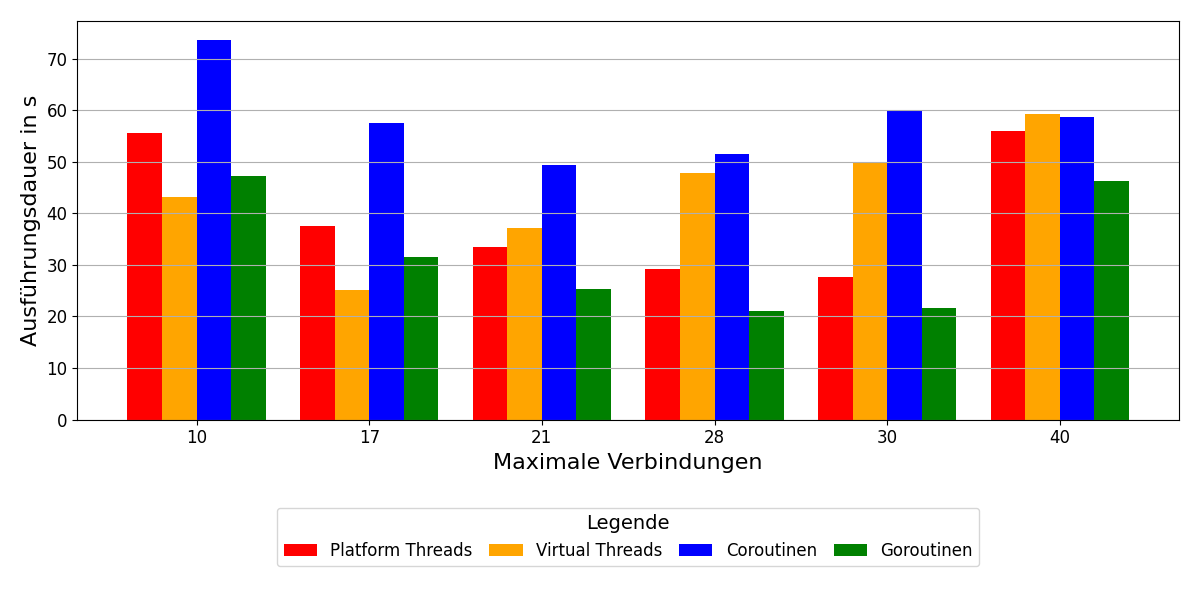
\includegraphics[scale=0.5]{figures/bank/connections10-40/execution_time_plot.png}
	\caption{Ausführungszeit pro Maximale Verbindungen,\\ Bank Messung 1: Maximale Verbindungen 10-40}
	\label{fig:bankConnZeit}
\end{figure}

Die Abbildung \ref{fig:bankConnZeit} zeigt die Ausführungszeit in Abhängigkeit der Anzahl an maximal zur Verfügung stehenden Datenbankverbindungen. Dabei liegen die optimalen Ausführungszeiten bei den oben genannten Werten. Des Weiteren hat sich gezeigt, dass die Schwankungen für alle Messparameter ab 40 maximal zur Verfügung stehenden Datenbankverbindungen aufhören. Jedoch auf einem deutlich höheren Niveau als bei ideal gewählten Verbindungszahlen.

\begin{figure}[H]
	\centering
	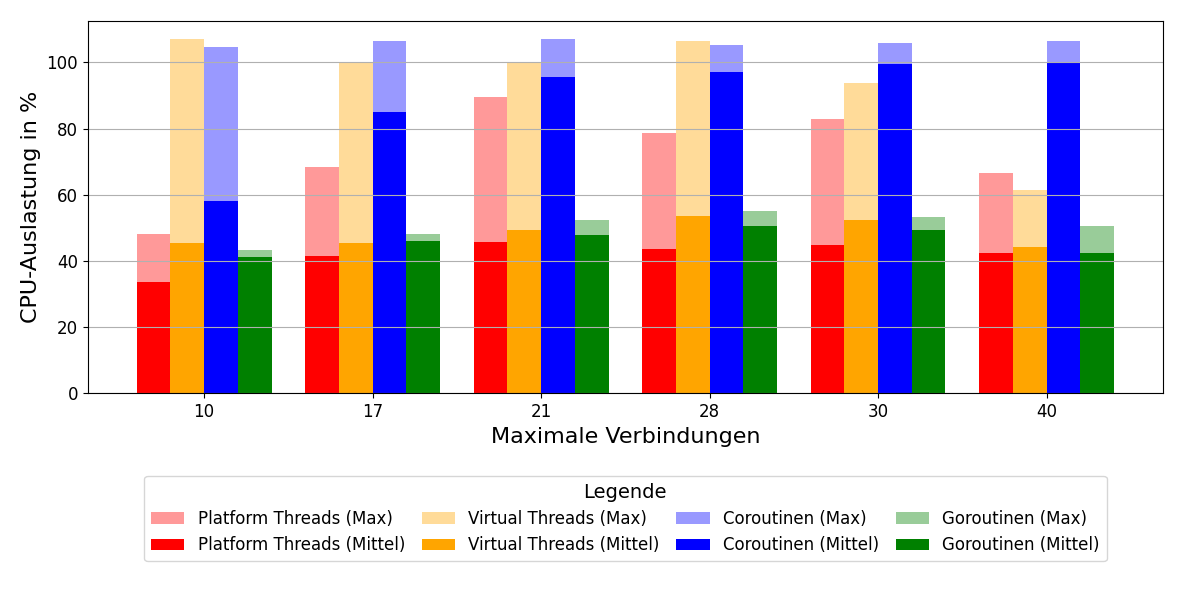
\includegraphics[scale=0.5]{figures/bank/connections10-40/cpu_usage_bar_plot.png}
	\caption{CPU-Auslastung pro Maximale Verbindungen,\\ Bank Messung 1: Maximale Verbindungen 10-40}
	\label{fig:bankConnCPU}
\end{figure}

Die Abbildung \ref{fig:bankConnCPU} zeigt die CPU-Auslastung der Bank-Benchmark Implementierungen in Abhängigkeit der Anzahl an maximal zur Verfügung stehenden Datenbankverbindungen. Es fällt auf, dass alle Implementierungen bis auf Coroutinen ungefähr 40-45\% der zur Verfügung stehenden CPU-Leistung benötigen. Im Gegensatz dazu weisen Coroutinen eine deutlich höhere CPU-Auslastung von 100\% auf. Diese Beobachtung lässt sich darauf zurückführen, dass Coroutinen R2DBC, einen reaktiven Ansatz, verwenden. Bei höheren maximalen Verbindungszahlen wird die CPU somit zum leistungslimitierenden Faktor für die Coroutinen-Implementierung.

\begin{figure}[H]
	\centering
	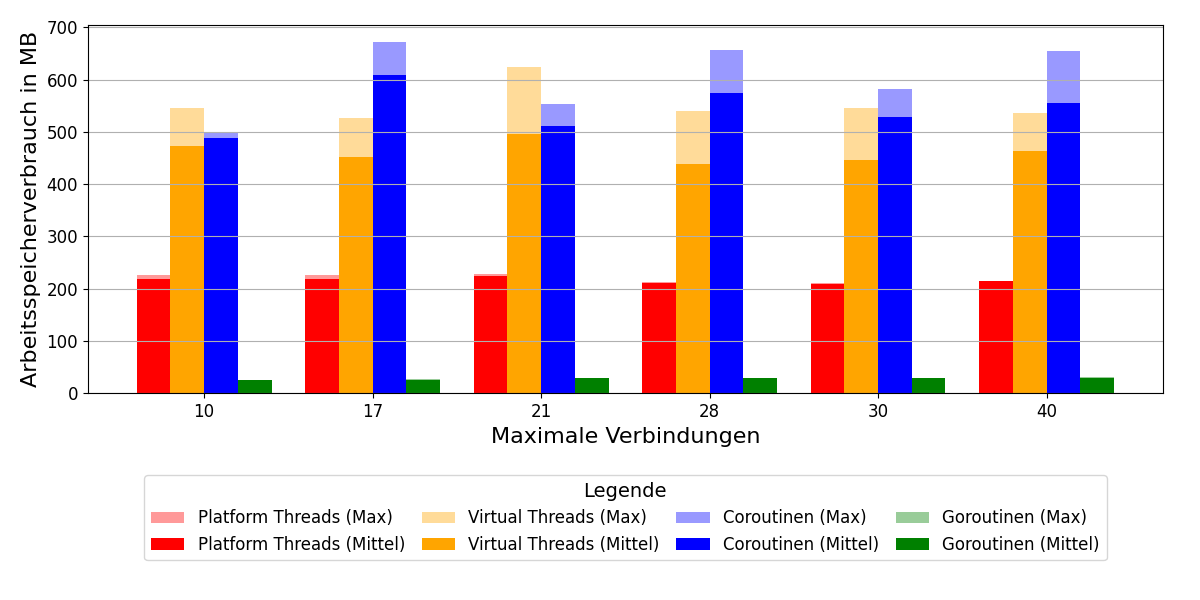
\includegraphics[scale=0.5]{figures/bank/connections10-40/memory_usage_bar_plot.png}
	\caption{Arbeitsspeicherverbrauch pro Maximale Verbindungen,\\ Bank Messung 1: Maximale Verbindungen 10-40}
	\label{fig:bankConnRAM}
\end{figure}

Die Abbildung \ref{fig:bankConnRAM} zeigt den Arbeitsspeicherverbrauch pro maximale Datenbankverbindungen für die verschiedenen Thread-Abstraktionen. Ein bemerkenswertes Merkmal dieser Darstellung ist die relative Konstanz der Werte über alle Messpunkte hinweg.

Unter den verglichenen Implementierungen weist Kotlin Coroutinen mit etwa 550 MB den höchsten Arbeitsspeicherverbrauch auf. Dicht dahinter folgen Java Virtual Threads mit ungefähr 450 MB. Java Platform Threads liegen mit circa 220 MB im mittleren Bereich. Go Goroutinen heben sich deutlich von den anderen Implementierungen ab und zeigen mit nur etwa 28 MB den mit Abstand niedrigsten Arbeitsspeicherverbrauch.

Trotz dieser erheblichen Unterschiede zwischen den verschiedenen Thread-Abstraktionen bleibt der jeweilige Arbeitsspeicherverbrauch über alle Messpunkte hinweg konstant. Dies lässt darauf schließen, dass der Arbeitsspeicherverbrauch eine charakteristische Eigenschaft der jeweiligen Implementierung ist und nicht von der Anzahl der maximalen Datenbankverbindungen beeinflusst wird, beziehungsweise diese nur einen kleinen Bruchteil ausmachen.

\begin{figure}[H]
	\centering
	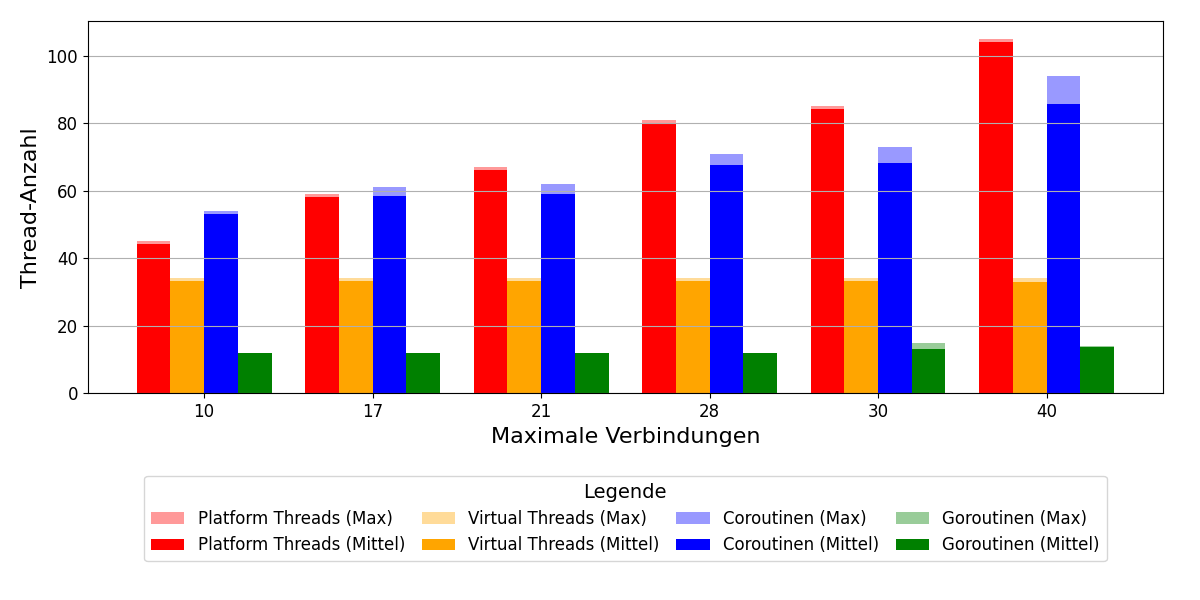
\includegraphics[scale=0.5]{figures/bank/connections10-40/num_threads_bar_plot.png}
	\caption{Thread-Anzahl pro Maximale Verbindungen,\\ Bank Messung 1: Maximale Verbindungen 10-40}
	\label{fig:bankConnThreads}
\end{figure}

Die Abbildung \ref{fig:bankConnThreads} zeigt die Thread-Anzahl der verschiedenen Bank-Benchmark Implementierungen in Abhängigkeit der maximal verfügbaren Datenbankverbindungen. Dabei fallen einige interessante Muster auf:
Virtual Threads und Goroutinen zeigen konstante Werte über alle Messpunkte hinweg. Virtual Threads verwendet durchgehend um die 33 Betriebssystem-Threads, während Goroutinen mit nur ca. 12 Betriebssystem-Threads auskommt. Diese Konstanz deutet auf eine erfolgreiche Entkopplung von den BS-Threads hin.

Platform Threads hingegen zeigen einen linearen Anstieg der Thread-Anzahl. Die Anzahl lässt sich durch die Formel \texttt{24+(maxConnections*2)} beschreiben, was auf die Verwendung von \texttt{Executors"".new""Fixed""Thread""Pool""(maxConnections*2)} zurückzuführen ist.

Coroutinen weisen ein anderes Verhalten auf. Die Thread-Anzahl steigt bis auf etwa 85 Threads an und stagniert dann zwischen 80 und 90 Threads, was sich mit Erfahrungen aus anderen Messungen deckt. Dieses Verhalten unterscheidet sich von den anderen drei Implementierungen, bei denen die maximalen gleichzeitigen Anfragen an den jeweiligen Pool auf \texttt{maxConnections*2} begrenzt sind. Bei Coroutinen gibt es keine solche Begrenzung dafür, wie viele Coroutinen gleichzeitig Anfragen an den R2DBC-Pool senden dürfen.

\begin{figure}[H]
	\centering
	\includegraphics[scale=0.5]{figures/bank/connections10-40/postgres\_cpu\_bar\_plot.png}
	\caption{PostgreSQL CPU-Auslastung pro Maximale Verbindungen,\\ Bank Messung 1: Maximale Verbindungen 10-40}
	\label{fig:bankConnPostgCPU}
\end{figure}

Die Abbildung \ref{fig:bankConnPostgCPU} zeigt die CPU-Auslastung der PostgreSQL-Datenbank in Abhängigkeit von der Anzahl der maximalen Datenbankverbindungen für verschiedene Thread-Abstrak\-tionen. Es fällt auf, dass mit Ausnahme der Coroutinen-Implementierung alle anderen untersuchten Implementierungen die Datenbank bei einer hohen Anzahl von Datenbankverbindungen vollständig auslasten können. Im Gegensatz dazu erreichen die Coroutinen nur eine maximale Auslastung der Datenbank von etwa 50\%. Diese Beobachtung lässt sich damit erklären, dass bei der Coroutinen-Implementierung die CPU-Auslastung der Anwendung selbst der limitierende Faktor ist.

\subsubsection{Messung 2: Bank - Verzögerung}

\begin{tabularx}{\textwidth}{@{}lX@{}}
	\textbf{Maximale Datenbankverbindungen:} & 80 \\
	\textbf{Anzahl der Bankkonten:} & 1000 \\
	\textbf{Anzahl der Überweisungen:} & 100.000 \\
	\textbf{Verzögerung der Überweisungen:} & \textbf{10-100 ms} \\
	\textbf{Implementierungen:} & Java Platform Threads, Java Virtual Threads, Kotlin Coroutinen, Go Goroutinen
\end{tabularx}

In der zweiten Messung des Bank-Benchmarks wurde untersucht, wie die verschiedenen Thread-Abstraktionen mit zunehmender Latenz der Datenbankoperationen umgehen. Die maximale Anzahl der Datenbankverbindungen wurde auf 80 festgelegt. Diese Einstellung wurde gewählt, um eine hohe Parallelität zu ermöglichen, ohne die standardmäßige Obergrenze von 100 Verbindungen in PostgreSQL zu überschreiten. Die Verzögerung der Über\-wei\-sun\-gen wurde durch die Verwendung von \texttt{pg\_sleep} in der Datenbank simuliert und variierte zwischen 10 und 100 Millisekunden.

Besonders interessant für die Analyse waren die Ausführungszeit sowie die CPU-Auslastung der verschiedenen Implementierungen.

\begin{figure}[H]
	\centering
	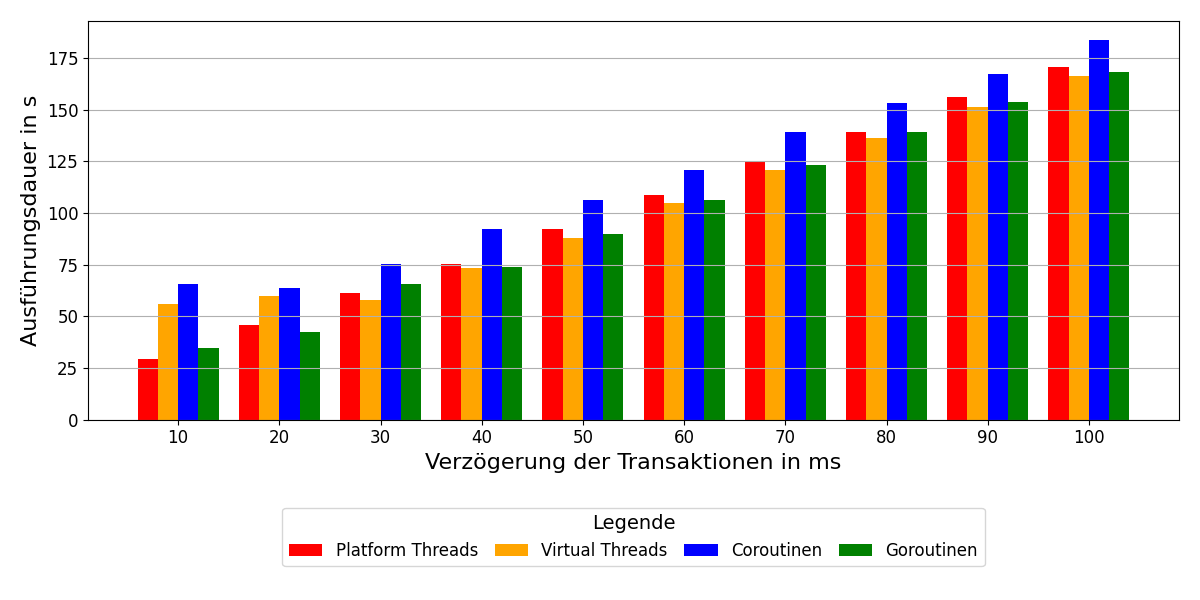
\includegraphics[scale=0.5]{figures/bank/delay80/execution_time_plot.png}
	\caption{Ausführungszeit pro Verzögerung,\\ Bank Messung 2: Verzögerung 10-100 ms}
	\label{fig:bankDelay80Zeit}
\end{figure}

Abbildung \ref{fig:bankDelay80Zeit} stellt die Ausführungszeit der verschiedenen Thread-Abstraktionen in Ab\-hän\-gig\-keit von der Verzögerung der Überweisungen dar. Die Grafik zeigt einen li\-ne\-aren Anstieg der Ausführungszeit für alle Implementierungen mit zunehmender Ver\-zö\-ge\-rung.

Bei geringen Verzögerungen weisen die Platform Threads zunächst die kürzeste Aus\-füh\-rungs\-zei\-t auf. Ab einer Verzögerung von etwa 30 Millisekunden ändert sich jedoch die Reihenfolge, und es stellt sich ein konsistentes Muster ein. Virtual Threads und Goroutinen zeigen dann die kürzesten Ausführungszeiten, dicht gefolgt von den Platform Threads. Die Coroutinen weisen durchgehend die längsten Ausführungszeiten auf, wenn auch der Abstand zu den anderen Implementierungen relativ gering bleibt.

Bemerkenswert ist, dass trotz der unterschiedlichen Leistungscharakteristika die Aus\-füh\-rungs\-zei\-ten aller getesteten Thread-Abstraktionen über den gesamten Ver\-zö\-ge\-rungs\-be\-reich hinweg recht nahe beieinander liegen.

\begin{figure}[H]
	\centering
	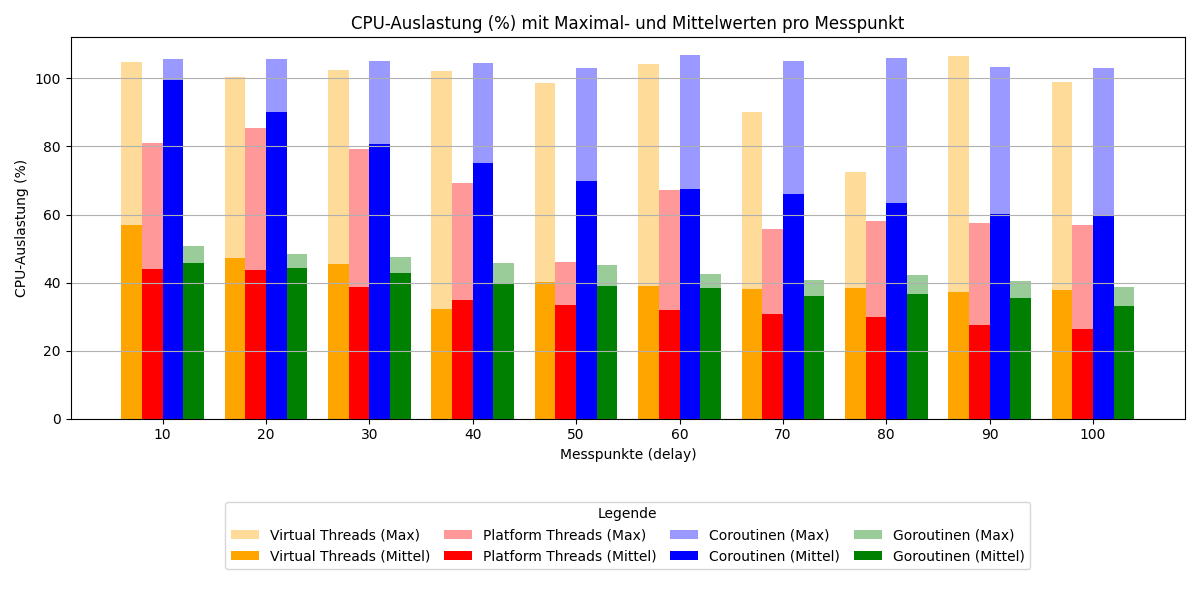
\includegraphics[scale=0.5]{figures/bank/delay80/cpu_usage_bar_plot.png}
	\caption{CPU-Auslastung pro Verzögerung,\\ Bank Messung 2: Verzögerung 10-100 ms}
	\label{fig:bankDelay80CPU}
\end{figure}

Abbildung \ref{fig:bankDelay80CPU} zeigt die CPU-Auslastung der verschiedenen Thread-Abstraktionen in Ab\-hän\-gig\-keit von der Verzögerung der Überweisungen. Bei einer Latenz von 10 Millisekunden liegen die CPU-Auslastungen für Platform Threads, Virtual Threads und Goroutinen eng beieinander, wobei Platform Threads die niedrigste Auslastung mit etwa 44\% und Virtual Threads die höchste mit etwa 56\% aufweisen. Auffällig ist, dass die Coroutinen-Implementierung bei dieser Latenz eine deutlich höhere CPU-Auslastung von 100\% zeigt, was mit den Ergebnissen aus der ersten Messung für eine hohe Anzahl maximaler Verbindungen übereinstimmt.

Mit zunehmender Verzögerung ist für alle Implementierungen ein leichter linearer Rück\-gang der CPU-Auslastung zu beobachten. Dieser Trend deutet darauf hin, dass bei längeren Wartezeiten zwischen den Überweisungen die Prozessorressourcen weniger intensiv genutzt werden. Die Coroutinen-Implementierung behält jedoch durchgehend die höchste CPU-Auslastung, während die anderen Thread-Abstraktionen weiterhin relativ dicht beieinander liegen.

Ein ähnliches Bild zeigt sich für die CPU-Auslastung der PostgreSQL-Datenbank, die ebenfalls mit steigender Latenz linear abnimmt (siehe Abb.: \ref{fig:bankDelay80PostgCPU}). 

Der Arbeitsspeicherverbrauch bleibt hingegen konstant und weist kaum Unterschiede zum Verbrauch in Messung 1 auf (siehe Abb.: \ref{fig:bankDelay80RAM}).

Die Thread-Anzahl bleibt ebenfalls konstant, was nicht überraschend ist, da mit festen Datenbankverbindungspools gearbeitet wird (siehe Abb.: \ref{fig:bankDelay80Threads}).

Bei Verwendung der jeweils idealen Anzahl an Verbindungen für die Implementierungen, die in Messung 1 ermittelt wurden, zeigt sich eine Verlagerung hinsichtlich der Implementierung mit den kürzesten Ausführungszeiten (siehe Abb.: \ref{fig:bankdelayIdealZeit}). Insgesamt sind jedoch alle Ausführungszeiten deutlich langsamer als bei 80 maximalen Verbindungen. Dies ist darauf zurückzuführen, dass die Parallelität durch die kleineren Pool-Größen deutlich begrenzter ist, was sich als Nachteil bei Latenzen in der Datenbankkommunikation erweist.

Abschließend lässt sich festhalten, dass Latenzen in der Kommunikation mit der Datenbank direkte Auswirkungen auf die Ausführungszeit haben. Zudem sinkt die CPU-Auslastung sowohl bei den Implementierungen als auch bei der PostgreSQL-Datenbank mit zunehmender Latenz.

Der Grund dafür liegt in der Limitierung durch den Datenbankverbindungspool, der zum begrenzenden Faktor für die Parallelität wird. Mit maximal 80 gleichzeitig ausführbaren Transaktionen reicht die Kapazität bei steigender Latenz nicht aus, um eine optimale Auslastung zu gewährleisten. Eine ideale Lösung wäre, wenn eine Verbindung freigegeben werden könnte, sobald eine Transaktion blockiert, sodass eine weitere Transaktion diese Verbindung nutzen könnte. Dies würde dem Prinzip der Thread-Abstraktionen ähneln, bei denen Ressourcen effizient wiederverwendet werden, wenn ein Thread oder eine Aufgabe auf eine I/O-Operation wartet.

\subsubsection{Messung 3: Bank - Anzahl an Überweisungen}

\begin{tabularx}{\textwidth}{@{}lX@{}}
	\textbf{Maximale Datenbankverbindungen:} & 80 \\
	\textbf{Anzahl der Bankkonten:} & 1000 \\
	\textbf{Anzahl der Überweisungen:} & \textbf{100.000 - 500.000} \\
	\textbf{Verzögerung der Überweisungen:} & 0.0 ms \\
	\textbf{Implementierungen:} & Java Platform Threads, Java Virtual Threads, Kotlin Coroutinen, Go Goroutinen
\end{tabularx}

In der dritten Messung des Bank-Benchmarks wurde untersucht, wie die verschiedenen Thread-Abstraktionen mit einer steigenden Anzahl von Überweisungen umgehen. Für diesen Test wurde die Anzahl der Überweisungen zwischen 100.000 und 500.000 variiert.

Die Messung wurde in zwei Varianten durchgeführt: Einmal mit einer maximalen Anzahl von 80 Datenbankverbindungen für alle Implementierungen und einmal unter den jeweils idealen Bedingungen, die in Messung 1 ermittelt wurden. Diese idealen Einstellungen waren 17 Verbindungen für Virtual Threads, 21 für Coroutinen, 28 für Goroutinen und 30 für Platform Threads.

Besonders interessant für die Analyse waren die Ausführungszeiten, sowohl für die Konfiguration mit 80 maximalen Verbindungen als auch für die idealen Einstellungen. Diese Zeiten geben Aufschluss darüber, wie gut die verschiedenen Thread-Abstraktionen mit einer zunehmenden Arbeitslast umgehen können.

\begin{figure}[H]
	\centering
	\includegraphics[scale=0.49]{figures/bank/transactions80/execution\_time\_plot.png}
	\caption{Ausführungszeit pro Anzahl an Überweisungen,\\ Bank Messung 3: Anzahl an Überweisungen 100.000-500.000}
	\label{fig:bankTransactions80Zeit}
\end{figure}

Abbildung \ref{fig:bankTransactions80Zeit} zeigt die Ausführungszeit pro Anzahl an Über\-wei\-sung\-en mit 80 maximalen Verbindungen für die verschiedenen Implementierungen. Es ist erkennbar, dass alle Implementierungen linear mit der steigenden Anzahl an Überweisungen skalieren. Besonders auffällig ist, dass die Coroutinen-Implementierung am besten skaliert und sich mit zunehmender Zahl an Überweisungen deutlich von den anderen drei Implementierungen absetzen kann.

\begin{figure}[H]
	\centering
	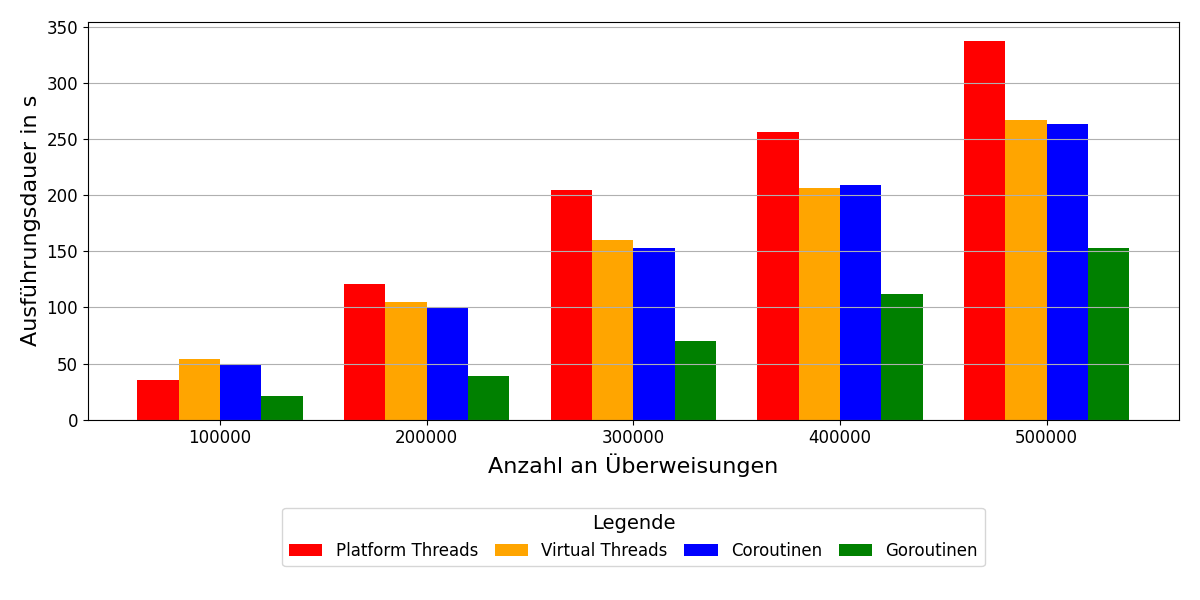
\includegraphics[scale=0.49]{figures/bank/transactionsIdeal/execution_time_plot.png}
	\caption{Ausführungszeit pro Anzahl an Überweisungen \\mit idealen Verbindungs-Einstellungen,\\ Bank Messung 3: Anzahl an Überweisungen 100.000-500.000}
	\label{fig:bankTransactionsIdealZeit}
\end{figure}

Im Vergleich dazu präsentiert Abbildung \ref{fig:bankTransactionsIdealZeit} die Ausführungszeit pro Anzahl an Über\-wei\-sun\-gen unter idealen Verbindungs-Einstellungen für jede Implementierung. Auch hier ist eine lineare Skalierung zu beobachten, jedoch bleibt das Verhältnis der Implementierungen zueinander nun weitgehend konstant. In dieser Konfiguration erweisen sich die Goroutinen als die schnellste Implementierung, mit einer, gegenüber den anderen, fast doppelt so schnellen Ausführungszeit. Virtual Threads und Coroutinen zeigen ähnliche Leistungen und liegen im Mittelfeld, während die Platform Threads die langsamste Performance aufweisen. Interessanterweise gibt es eine Ausnahme beim ersten Messpunkt, wo die Platform Threads die zweitschnellste Ausführungszeit verzeichnen.

Die restlichen Messwerte bleiben unauffällig. Es lässt sich beobachten, dass die CPU-Aus\-las\-tung für alle Implementierungen konstant bleibt (Abb.: \ref{fig:bankTransactions80CPU}), unabhängig von der steigenden Anzahl der Überweisungen. Ebenso bleibt die Thread-Anzahl über den gesamten Messbereich hinweg unverändert (\ref{fig:bankTransactions80Threads}). Die PostgreSQL CPU-Auslastung zeigt ebenfalls ein konstantes Verhalten (Abb.: \ref{fig:bankTransactions80PostgCPU}).

Der Arbeitsspeicherverbrauch weist einen langsamen, linearen Anstieg auf (Abb.: \ref{fig:bankTransactions80RAM}). Dies lässt sich dadurch erklären, dass mit steigender Anzahl der Überweisungen mehr Daten zu Beginn des Programms importiert werden müssen, was zu einem erhöhten Speicherbedarf führt.

Insgesamt lässt sich feststellen, dass die Anzahl der Überweisungen keinen signifikanten Einfluss auf die Performance-Metriken hat, mit Ausnahme der Ausführungszeit. Diese skaliert gleichmäßig mit der steigenden Anzahl der Überweisungen. Interessanterweise führt ein möglichst hoher Grad an Parallelisierung nicht automatisch zu besseren Laufzeiten. Wie bereits in Messung 1 beobachtet, werden die besten Ergebnisse für die Ausführungszeit bei ideal gewählten Werten für die maximalen Verbindungen erzielt.

\subsubsection{Messung 4: Bank - Anzahl an Bankkonten}

\begin{tabularx}{\textwidth}{@{}lX@{}}
	\textbf{Maximale Datenbankverbindungen:} & 80 \\
	\textbf{Anzahl der Bankkonten:} & \textbf{10, 100, 1000, 10000} \\
	\textbf{Anzahl der Überweisungen:} & 100.000 \\
	\textbf{Verzögerung der Überweisungen:} & 0.0 ms \\
	\textbf{Implementierungen:} & Java Platform Threads, Java Virtual Threads, Kotlin Coroutinen, Go Goroutinen
\end{tabularx}

Die vierte Messung des Bank-Benchmarks untersucht den Einfluss der Anzahl der Bankkonten auf die Performance der verschiedenen Thread-Abstraktionen. Für diesen Test wurde die Anzahl der Bankkonten von 10 bis 10.000 variiert, während die anderen Parameter konstant blieben.

Es ist wichtig zu beachten, dass die Anzahl der Bankkonten der Anzahl der Zeilen in der PostgreSQL-Tabelle entspricht. Bei einer Überweisung werden zwei Zeilen gesperrt, da sowohl das Sender- als auch das Empfängerkonto betroffen sind. Daraus folgt, dass die maximale Anzahl gleichzeitiger Transaktionen der Hälfte der Anzahl der Konten entspricht. Dies erklärt die längeren Ausführungszeiten bei einer geringen Anzahl von Konten, da dies zum begrenzenden Faktor wird.

Insgesamt zeigt diese Messung, dass die Anzahl der Bankkonten keine nennenswerten Auswirkungen auf die Performance hat, solange sie ausreichend groß gewählt wird. Die detaillierten Ergebnisse und Graphen können im Anhang eingesehen werden (Abschnitt: \ref{subsec:bank4graph}).

\subsubsection{Fazit: Bank}

Der Bank-Benchmark zeigt, dass die Performance von Thread-Abstraktionen stark von anderen Technologien abhängt, insbesondere von der Datenbank, dem Datenbanktreiber und dem Datenbankverbindungspool. Um das volle Potenzial der Thread-Abstraktionen auszuschöpfen, müssen all diese Komponenten die jeweiligen Thread-Abstraktionen unterstützen.

Die Leistung ist dementsprechend stark von den genutzten Technologien abhängig. Da Virtual Threads noch relativ neu sind, müssen andere Technologien nachziehen oder weiter optimiert werden, um das volle Potenzial der Virtual Threads ausnutzen zu können.

Ein generelles Problem, das sich herauskristallisierte, ist die fehlende Entkopplung bei Datenbankverbindungen, ähnlich wie sie bei Thread-Abstraktionen existiert. Dies begrenzt den Nutzen der Freigabe von Threads erheblich, da die maximale Anzahl an Verbindungen zum limitierenden Faktor für die Parallelität wird. Besonders deutlich wurde dies in der zweiten Messung mit künstlichen Latenzen in den Überweisungen. Hier stand theoretisch noch CPU-Leistung zur Verfügung, die aufgrund dieser Begrenzung nicht ausgeschöpft werden konnte.

Interessanterweise hat sich gezeigt, dass bei geringen Latenzen, also wenigen oder kurzen Blockierungen, ein hoher Grad an Parallelisierung nicht vorteilhaft ist. Die erste Messung demonstrierte sogar, dass die idealen Werte für maximale Verbindungen eher niedrig sind. Dies deutet darauf hin, dass es in solchen Szenarien wichtiger ist, den Overhead gering zu halten, als die Parallelität zu steigern.

\chapter{Zusammenfassung und Ausblick}

\section{Fazit}

Im ersten Teil dieser Arbeit wurde eine tiefgehende Recherche zu den Thread-Abstraktionen durchgeführt, die es ermöglichte, die theoretischen Konzepte der Technologien gegen\-über\-zu\-stellen. Dabei wurden Gemeinsamkeiten und Unterschiede in ihrer Funktionsweise sowie deren Stärken und Schwächen analysiert und miteinander verglichen:

Die drei neuen Thread-Abstraktionen der untersuchten Programmiersprachen (Java, Kotlin, Go) verfolgen einen ähnlichen Ansatz: Sie entkoppeln die Ausführung von Aufgaben von den Betriebssystem-Threads. Dies bedeutet, dass die Anzahl der gleichzeitig ausführbaren Aufgaben nicht mehr, wie bei Java Platform Threads, direkt an die Anzahl der verfügbaren Betriebssystem-Threads gebunden ist. Stattdessen wird ein Scheduling auf Laufzeitebene eingeführt, das es ermöglicht, eine deutlich größere Zahl von leichtgewichtigen Thread-Abstraktionen (wie Virtual Threads, Coroutinen oder Goroutinen) auf einer kleineren Anzahl von Betriebssystem-Threads zu verwalten.

Diese Entkopplung führt zu einem geringeren Ressourcenverbrauch, da nicht für jede parallel auszuführende Aufgabe ein eigener Betriebssystem-Thread erstellt werden muss. Dadurch können Anwendungen eine erheblich höhere Anzahl von gleichzeitigen Aufgaben effizient verwalten, was besonders bei I/O-lastigen Operationen von Vorteil ist, da diese oft blockieren.

Diese theoretische Grundlage wurde im zweiten Teil der Arbeit durch Benchmarks praktisch überprüft, um die Konzepte unter realistischen Bedingungen zu evaluieren. Ziel war es, die theoretischen Annahmen durch konkrete Messungen zu verifizieren oder zu falsifizieren und die tatsächliche Leistungsfähigkeit der Thread-Abstraktionen zu bewerten:

Diese theoretischen Effizienzsteigerungen wurde im Rahmen des ersten Benchmarks (Mergesort) deutlich demonstriert, insbesondere in den Messungen 2 und 3, bei denen gezielt viele Threads erstellt wurden. Die neuen Versionen zeigten sich deutlich länger performant als die alten Platform Threads. Bei ihnen blieb die Anzahl der Betriebssystem-Threads bis zum Schluss konstant niedrig blieb, während die Anzahl der Platform Threads stetig anstieg. 

Allerdings zeigte die erste Messung des Mergesort-Benchmarks auch, dass nach einer optimalen CPU-Auslastung, mit einen geringen Grad an Parallelisierung, keine weiteren Laufzeitvorteile erzielt werden konnten.

Der zweite Benchmark (Bank) offenbarte eine starke Abhängigkeit von anderen Technologien, die die neuen Thread-Abstraktionen unterstützen müssen. Selbst bei vorhandener Unterstützung konnte kein signifikanter Performancegewinn erzielt werden. Es wurde sichtbar, dass da eine Entkopplung von Datenbankverbindungen und Transaktionen mit den genutzten Technologien zurzeit nicht technisch möglich ist.

Ein zweiter zentraler Befund des Bank-Benchmarks ist, dass höhere Parallelisierung nicht automatisch bessere Performance bedeutet. Bei niedrigen Latenzen oder wenigen Blockierungen überwiegt der Verwaltungsaufwand vieler Datenbankverbindungen oft die Vorteile höherer Parallelisierung. Effiziente Ressourcennutzung und optimal abgestimmte Verbindungen sind entscheidender als die bloße Erhöhung paralleler Aufgaben.

Die neuen Thread-Abstraktionen zeigen ihre Stärken besonders in Szenarien mit hoher Parallelität in Kombination mit häufigen Unterbrechungen. Sie bieten mindestens die gleiche Leistung wie die alten Implementierungen, übertreffen diese jedoch deutlich in der beschrieben Situationen. 

Generell lässt sich festhalten, dass die neuen Thread-Abstraktionen in keinem Fall schlechter abschneiden als die alten. Dies ermöglicht beispielsweise in Java einen bedenkenlose Umstellung von Platform Threads auf Virtual Threads. Die neuen Virtual Threads konnten in den Benchmarks sogar besser abschneiden als ihr direktes Konkurrenzprodukt in der JVM, die Kotlin Coroutinen.

Trotz dieser Fortschritte zeigten die Goroutinen in Go mit Abstand die beste Performance, was nicht überrascht, da Go von Grund auf für Leistung und Nebenläufigkeit entwickelt wurde.


\section{Ausblick}

Die vorliegende Masterarbeit bietet eine solide Grundlage für weiterführende Untersuchungen im Bereich der Nebenläufigkeit und Thread-Abstraktionen in verschiedenen Programmiersprachen. Es gibt mehrere vielversprechende Anknüpfungspunkte, die das Potenzial haben, die Arbeit zu erweitern und zu vertiefen und durch Entwicklung eines robusten Testaufbaus inklusive entsprechender Messwerkzeuge ist dies mit einem überschaubaren Aufwand möglich.

Ein wichtiger Bereich für zukünftige Forschung wäre die Erweiterung um weitere Benchmarks. Dabei gibt es verschiedene interessante Ansätze:

Insbesondere wäre es interessant zu untersuchen ob es eine Möglichkeit zur Entkopplung von Transaktionen und Datenbankverbindungen gibt, ähnlich wie sie bei Thread-Abstraktionen existiert. Eine mögliche Lösung wäre die Entwicklung eines "Connection Pooling"-Systems, das Datenbankverbindungen ähnlich verwaltet wie Goroutinen oder Virtual Threads. Dieses System könnte eine große Anzahl von virtuellen Datenbankverbindungen auf eine begrenzte Anzahl tatsächlicher Verbindungen abbilden. Dadurch würde die Limitierung durch die maximale Anzahl an Datenbankverbindungen umgangen und die volle Leistungsfähigkeit der Thread-Abstraktionen könnte ausgeschöpft werden.

Des weiteren könnte die Untersuchung von Cancellation-Mechanismen wertvolle Einblicke liefern. Diese werden in den Sprachen unterschiedlich umgesetzt. Coroutinen nutzen Coroutinen-Scopes zur Ermöglichung einer hierarchischen Strukturierung, Goroutinen hingegen das Closing-Channels-Programmiermuster.
Für Java Virtual Threads wird zukünftig vermutlich die sogenannte Structured Concurrency eingeführt, welche ebenfalls eine Hierarchie unter den Virtual Threads ermöglicht.

Ein weiterer wichtiger Aspekt für zukünftige Untersuchungen wäre das Exception Handling. Eine detaillierte Analyse des Verhaltens bei Ausnahmen und Abbrüchen in nebenläufigen Szenarien könnte die Robustheit verschiedener Implementierungen aufzeigen.

Zudem könnte die Entwicklung eines Webservers nach dem Thread-per-Request Modell Erkenntnisse für praktische Anwendungsfälle liefern und die Effizienz der verschiedenen Thread-Abstraktionen in realen Szenarien demonstrieren.

Um ein noch umfassenderes Bild zu erhalten, wäre es alternativ auch möglich, die vorhandenen Benchmarks auf weitere Programmiersprachen mit entsprechenden Thread-Abs\-trak\-tio\-nen auszuweiten. Insbesondere könnten Sprachen wie C++ und Rust in Betracht gezogen werden, die ihre eigenen Ansätze zur Nebenläufigkeit bieten.

Insgesamt bietet diese Masterarbeit ein gutes Fundament für potenziell weitere Untersuchungen. Die gewonnenen Erkenntnisse können als Ausgangspunkt für tiefergehende Analysen und praktische Anwendungen in der Softwareentwicklung dienen.


\printbibliography


\chapter{Anhang}

\section{Mergesort: zusätzliche Graphen}

\subsection{Mergesort Messung 2: Graphen}

\begin{figure}[H]
	\centering
	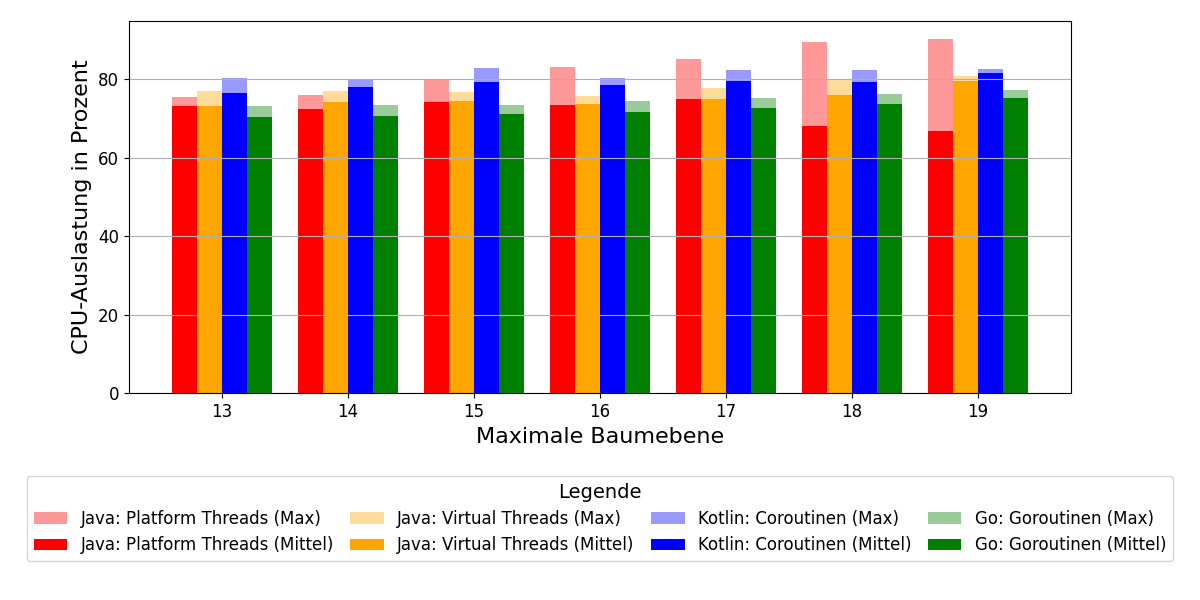
\includegraphics[scale=0.5]{figures/mergesort/Maximalebauebenen1-19_pvcg/cpu_usage_bar_plot.png}
	\caption{CPU-Auslastung pro maximaler Baumebene,\\ Mergesort Messung 2: max. Baumebenen 13-19}
	\label{fig:ms1-19CPU}
\end{figure}

\begin{figure}[H]
	\centering
	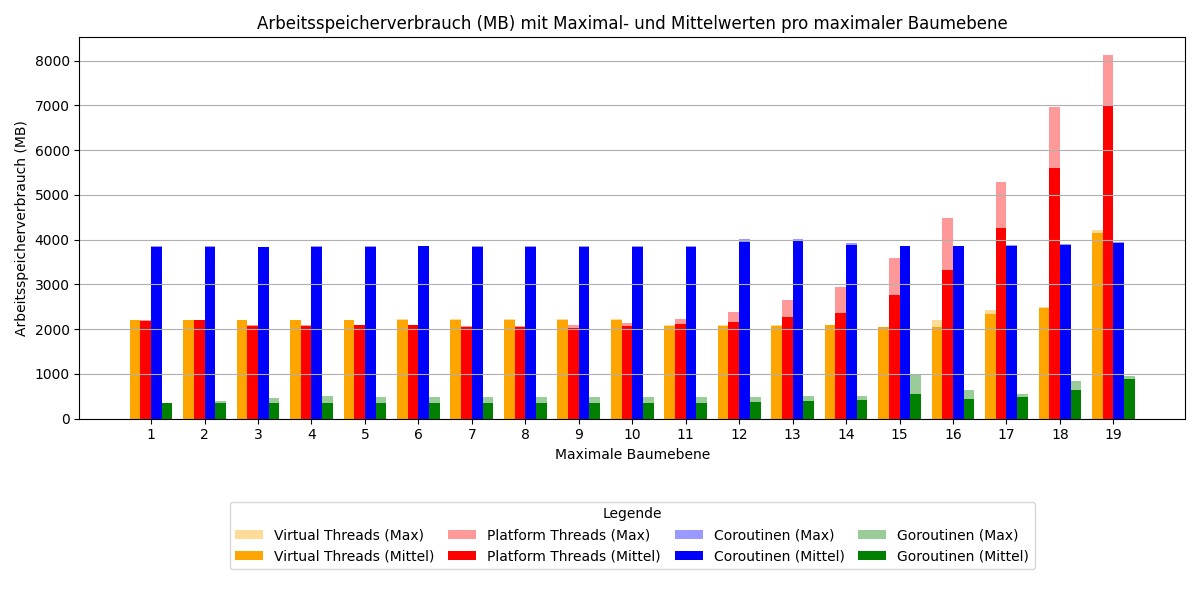
\includegraphics[scale=0.5]{figures/mergesort/Maximalebauebenen1-19_pvcg/memory_usage_bar_plot.png}
	\caption{Arbeitsspeicherverbrauch pro maximaler Baumebene,\\ Mergesort Messung 2: max. Baumebenen 13-19}
	\label{fig:ms1-19RAM}
\end{figure}

\subsection{Mergesort Messung 3: Graphen}

\begin{figure}[H]
	\centering
	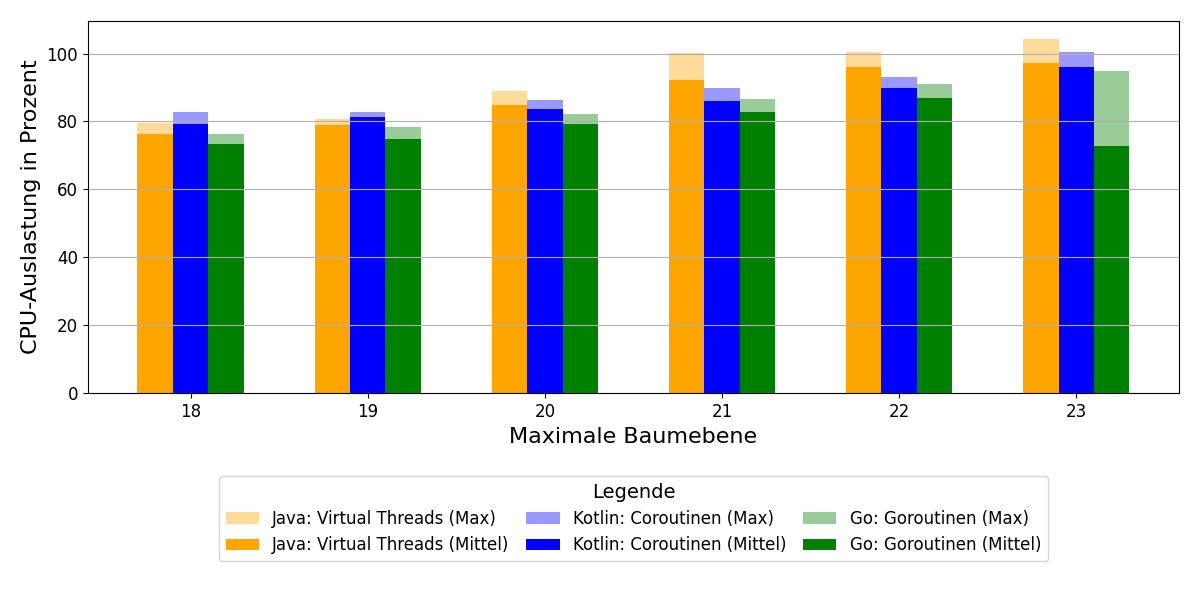
\includegraphics[scale=0.5]{figures/mergesort/Maximalebauebenen1-23_vcg/cpu_usage_bar_plot.png}
	\caption{CPU-Auslastung pro maximaler Baumebene,\\ Mergesort Messung 3: max. Baumebenen 18-23}
	\label{fig:ms1-23CPU}
\end{figure}

\begin{figure}[H]
	\centering
	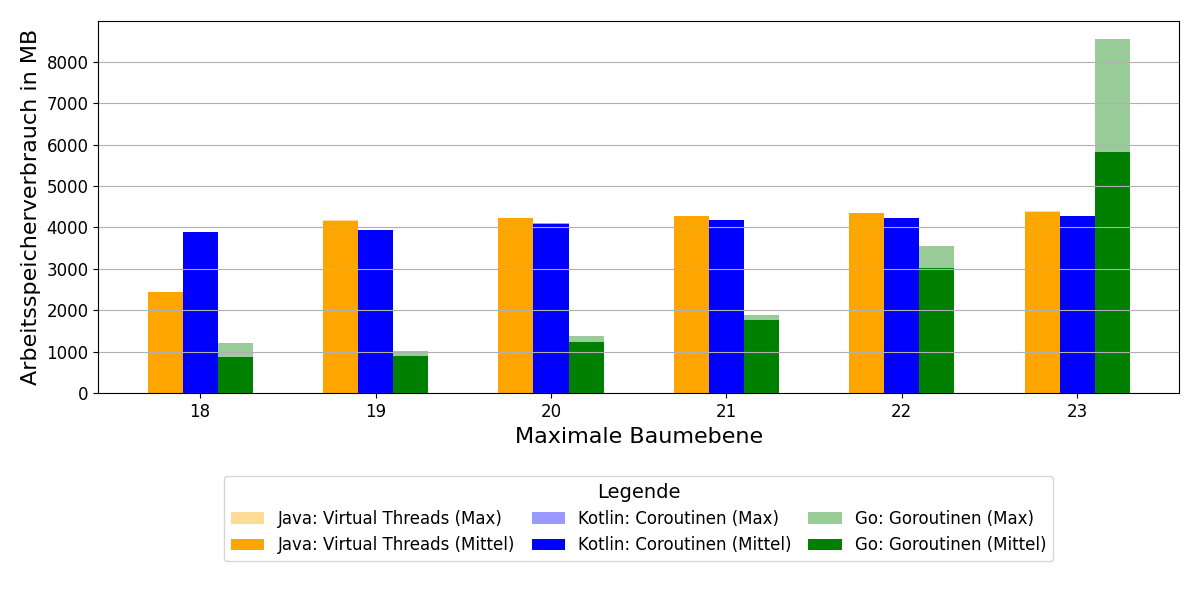
\includegraphics[scale=0.5]{figures/mergesort/Maximalebauebenen1-23_vcg/memory_usage_bar_plot.png}
	\caption{Arbeitsspeicherverbrauch pro maximaler Baumebene,\\ Mergesort Messung 3: max. Baumebenen 18-23}
	\label{fig:ms1-23RAM}
\end{figure}

\subsection{Mergesort Messung 4: Graphen}
\label{subsec:mergsort4graph}

\begin{figure}[H]
	\centering
	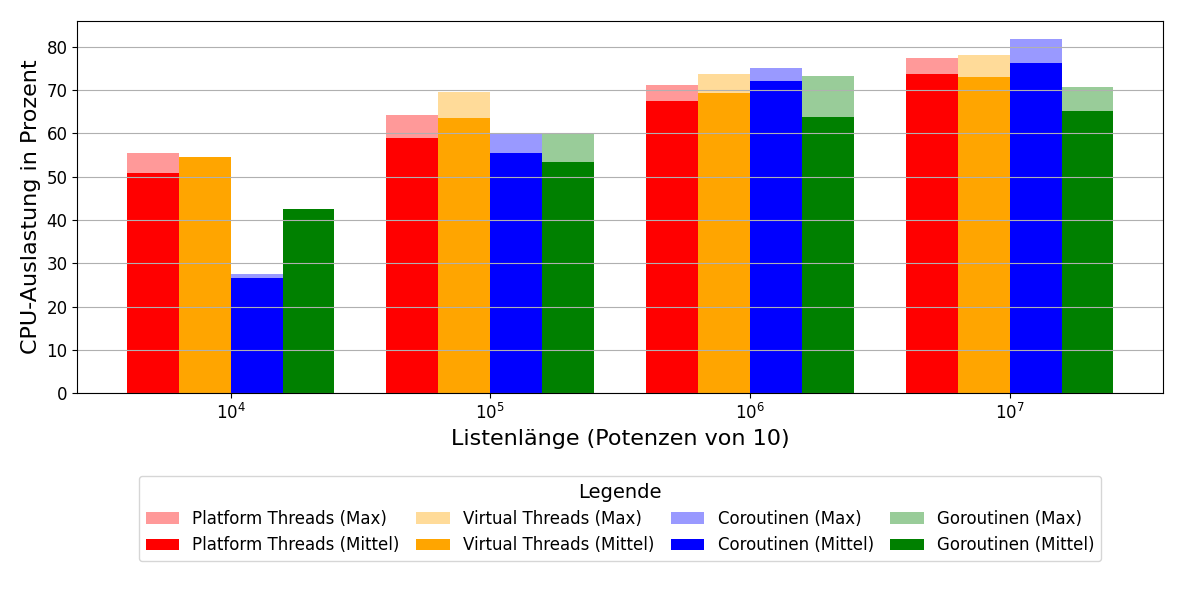
\includegraphics[scale=0.5]{figures/mergesort/Listenlaenge/cpu_usage_bar_plot.png}
	\caption{CPU-Auslastung pro Listenlänge,\\ Mergesort Messung 4: Listenlänge 10.000-10.000.000}
	\label{fig:mslaengeCPU}
\end{figure}

\begin{figure}[H]
	\centering
	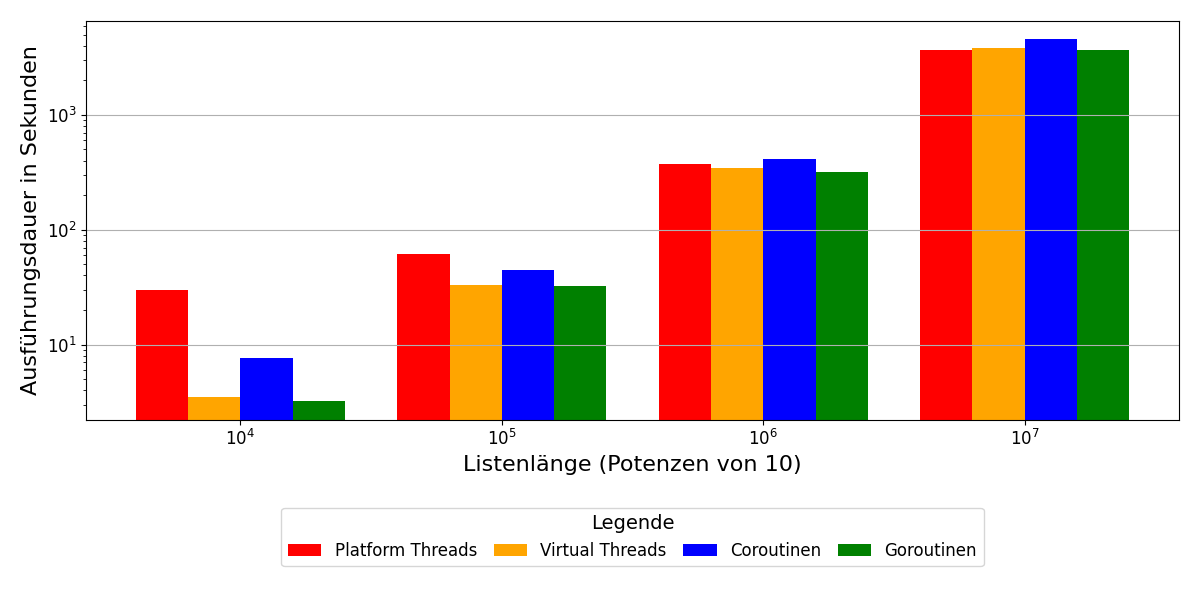
\includegraphics[scale=0.5]{figures/mergesort/Listenlaenge/execution_time_plot.png}
	\caption{Ausführungszeit pro Listenlänge,\\ Mergesort Messung 4: Listenlänge 10.000-10.000.000}
	\label{fig:mslaengeZeit}
\end{figure}

\begin{figure}[H]
	\centering
	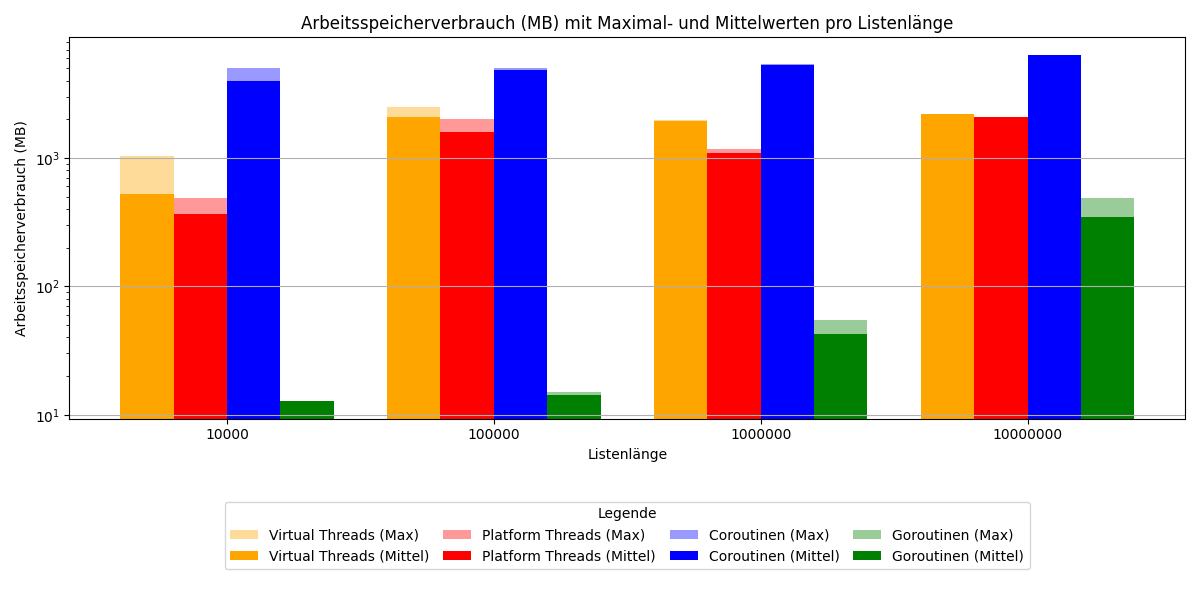
\includegraphics[scale=0.5]{figures/mergesort/Listenlaenge/memory_usage_bar_plot.png}
	\caption{Arbeitsspeicherverbrauch pro Listenlänge,\\ Mergesort Messung 4: Listenlänge 10.000-10.000.000}
	\label{fig:mslaengeRAM}
\end{figure}

\begin{figure}[H]
	\centering
	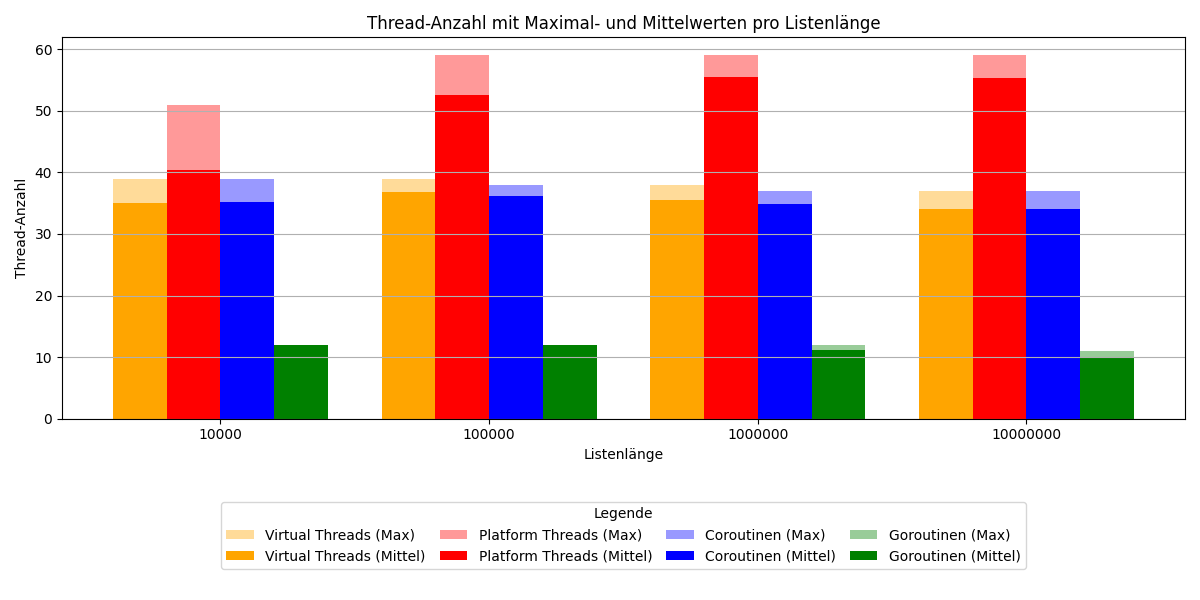
\includegraphics[scale=0.5]{figures/mergesort/Listenlaenge/num_threads_bar_plot.png}
	\caption{Thread-Anzahl pro Listenlänge,\\ Mergesort Messung 4: Listenlänge 10.000-10.000.000}
	\label{fig:mslaengeThreads}
\end{figure}

\section{Bank: zusätzliche Graphen}

\subsection{Bank Messung 2: Graphen}

\begin{figure}[H]
	\centering
	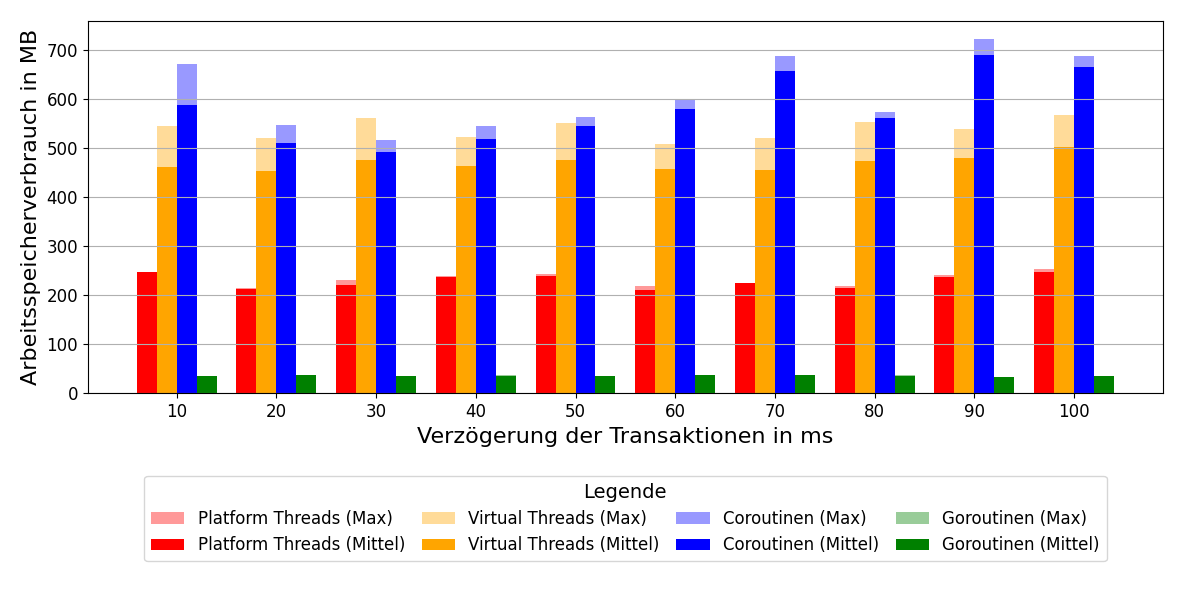
\includegraphics[scale=0.5]{figures/bank/delay80/memory_usage_bar_plot.png}
	\caption{Arbeitsspeicherverbrauch pro Verzögerung,\\ Bank Messung 2: Verzögerung 10-100 ms}
	\label{fig:bankDelay80RAM}
\end{figure}

\begin{figure}[H]
	\centering
	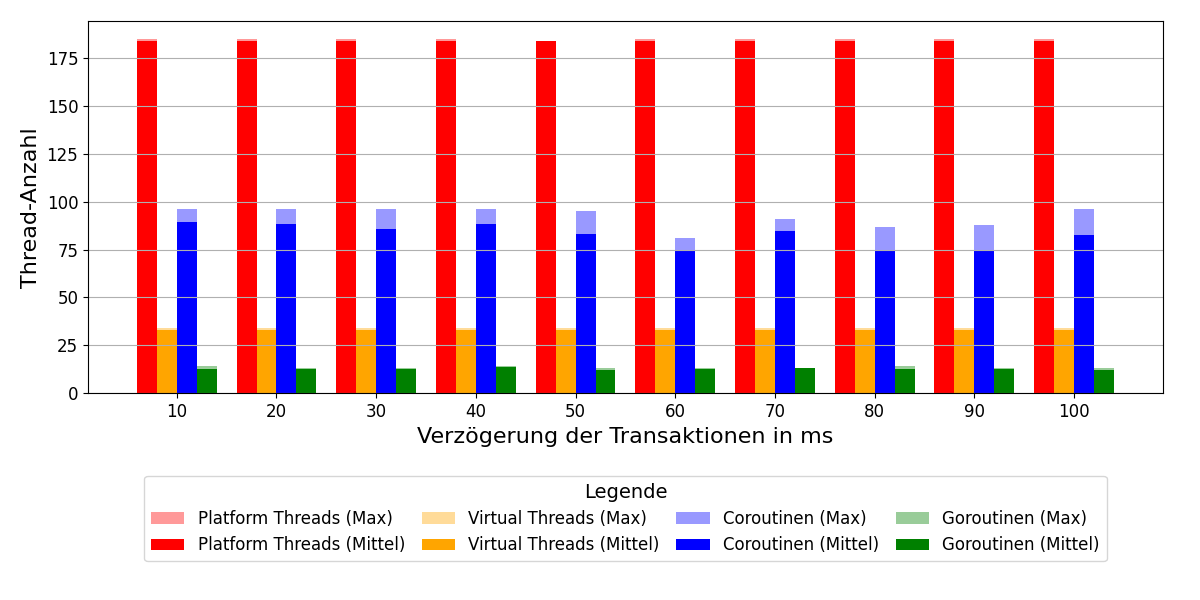
\includegraphics[scale=0.5]{figures/bank/delay80/num_threads_bar_plot.png}
	\caption{Thread-Anzahl pro Verzögerung,\\ Bank Messung 2: Verzögerung 10-100 ms}
	\label{fig:bankDelay80Threads}
\end{figure}

\begin{figure}[H]
	\centering
	\includegraphics[scale=0.5]{figures/bank/delay80/postgres\_cpu\_bar\_plot.png}
	\caption{PostgreSQL CPU-Auslastung pro Verzögerung,\\ Bank Messung 2: Verzögerung 10-100 ms}
	\label{fig:bankDelay80PostgCPU}
\end{figure}

\begin{figure}[H]
	\centering
	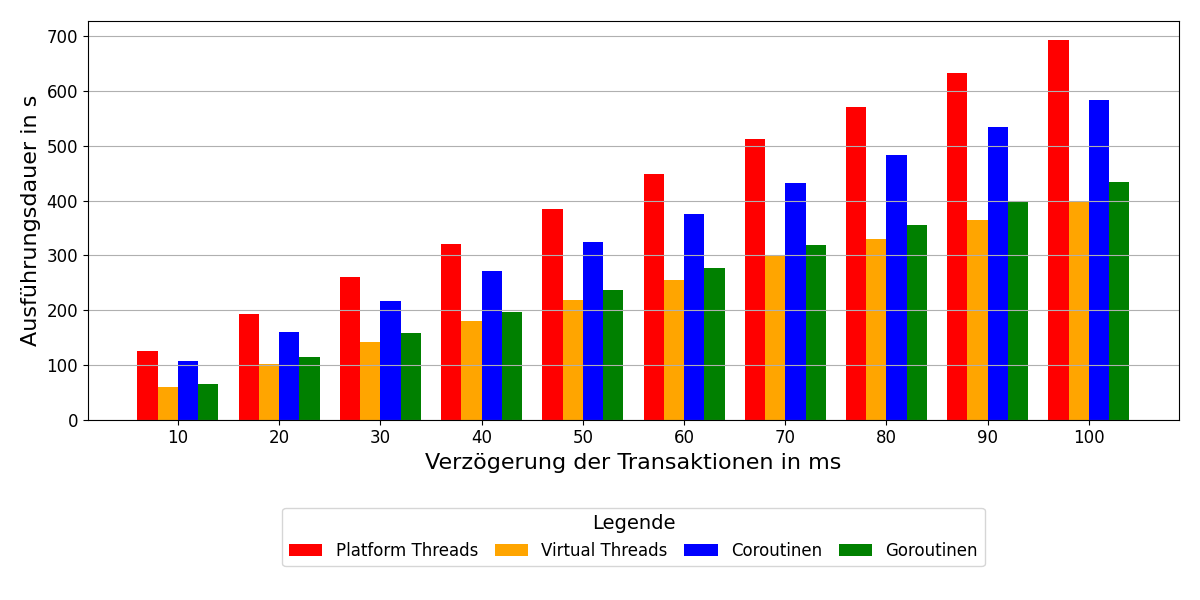
\includegraphics[scale=0.5]{figures/bank/delayIdeal/execution_time_plot.png}
	\caption{Ausführungszeit pro Verzögerung mit idealen Verbindungs-Einstellungen,\\ Bank Messung 2: Verzögerung 10-100 ms}
	\label{fig:bankdelayIdealZeit}
\end{figure}

\subsection{Bank Messung 3: Graphen}

\begin{figure}[H]
	\centering
	\includegraphics[scale=0.5]{figures/bank/transactions80/cpu\_usage\_bar\_plot.png}
	\caption{CPU-Auslastung pro Anzahl an Überweisungen,\\ Bank Messung 3: Anzahl an Überweisungen 100.000-500.000}
	\label{fig:bankTransactions80CPU}
\end{figure}

\begin{figure}[H]
	\centering
	\includegraphics[scale=0.5]{figures/bank/transactions80/memory\_usage\_bar\_plot.png}
	\caption{Arbeitsspeicherverbrauch pro Anzahl an Überweisungen,\\ Bank Messung 3: Anzahl an Überweisungen 100.000-500.000}
	\label{fig:bankTransactions80RAM}
\end{figure}

\begin{figure}[H]
	\centering
	\includegraphics[scale=0.5]{figures/bank/transactions80/num\_threads\_bar\_plot.png}
	\caption{Thread-Anzahl pro Anzahl an Überweisungen,\\ Bank Messung 3: Anzahl an Überweisungen 100.000-500.000}
	\label{fig:bankTransactions80Threads}
\end{figure}

\begin{figure}[H]
	\centering
	\includegraphics[scale=0.5]{figures/bank/transactions80/postgres\_cpu\_bar\_plot.png}
	\caption{PostgreSQL CPU-Auslastung pro Anzahl an Überweisungen,\\ Bank Messung 3: Anzahl an Überweisungen 100.000-500.0000}
	\label{fig:bankTransactions80PostgCPU}
\end{figure}

\subsection{Bank Messung 4: Graphen}
\label{subsec:bank4graph}

\begin{figure}[H]
	\centering
	\includegraphics[scale=0.5]{figures/bank/accounts80/execution\_time\_plot.png}
	\caption{Ausführungszeit pro Anzahl an Bankkonten,\\ Bank Messung 4: Anzahl an Bankkonten 10-10.000}
	\label{fig:bankAccounts80Zeit}
\end{figure}

\begin{figure}[H]
	\centering
	\includegraphics[scale=0.5]{figures/bank/accounts80/cpu\_usage\_bar\_plot.png}
	\caption{CPU-Auslastung pro Anzahl an Bankkonten,\\ Bank Messung 4: Anzahl an Bankkonten 10-10.000}
	\label{fig:bankAccounts80CPU}
\end{figure}

\begin{figure}[H]
	\centering
	\includegraphics[scale=0.5]{figures/bank/accounts80/memory\_usage\_bar\_plot.png}
	\caption{Arbeitsspeicherverbrauch pro Anzahl an Bankkonten,\\ Bank Messung 4: Anzahl an Bankkonten 10-10.000}
	\label{fig:bankAccounts80RAM}
\end{figure}

\begin{figure}[H]
	\centering
	\includegraphics[scale=0.5]{figures/bank/accounts80/num\_threads\_bar\_plot.png}
	\caption{Thread-Anzahl pro Anzahl an Bankkonten,\\ Bank Messung 4: Anzahl an Bankkonten 10-10.000}
	\label{fig:bankAccounts80Threads}
\end{figure}

\begin{figure}[H]
	\centering
	\includegraphics[scale=0.5]{figures/bank/accounts80/postgres\_cpu\_bar\_plot.png}
	\caption{PostgreSQL CPU-Auslastung pro Anzahl an Bankkonten,\\ Bank Messung 4: Anzahl an Bankkonten 10-10.000}
	\label{fig:bankAccounts80PostgCPU}
\end{figure}

\begin{figure}[H]
	\centering
	\includegraphics[scale=0.5]{figures/bank/accountsIdeal/execution_time_plot.png}
	\caption{Ausführungszeit pro Anzahl an Bankkonten \\mit idealen Verbindungs-Einstellungen, \\Bank Messung 4: Anzahl an Bankkonten 10-10.000}
	\label{fig:bankAccountsIdealZeit}
\end{figure}

\section{Mergesort Tabellen}

\subsection{Mergesort Messung 1: Tabellen}

\begin{table}[H]
	\centering
	\renewcommand{\arraystretch}{1.2} % Erhöhte Zeilenhöhe
	\rowcolors{2}{gray!10}{white} % Alternierende Zeilenfarben ab der zweiten Zeile
	\begin{tabularx}{\textwidth}{XXXXXXXXX} % 9 gleichmäßig verteilte Spalten
		\toprule
		\rowcolor{gray!20} % Kopfzeile farbig
		\textbf{\makecell[l]{Max \\ Baum- \\ ebene}} & 
		\textbf{\makecell[l]{JVT \\ Max \\ CPU}} & 
		\textbf{\makecell[l]{JVT \\ Mittel \\ CPU}} & 
		\textbf{\makecell[l]{JPT \\ Max \\ CPU}} & 
		\textbf{\makecell[l]{JPT \\ Mittel \\ CPU}} & 
		\textbf{\makecell[l]{Coro\\ Max \\ CPU}} & 
		\textbf{\makecell[l]{Coro\\ Mittel \\ CPU}} & 
		\textbf{\makecell[l]{Goro\\ Max \\ CPU}} & 
		\textbf{\makecell[l]{Goro\\ Mittel \\ CPU}} \\
		\midrule
		\csvreader[
		head to column names,
		late after line=\\
		]{measurements/mergesort/Maximalebauebenen1-6/cpu_usage_aggregated.csv}{}
		{\csvcoli & 
			\pgfmathparse{\csvcolii}\pgfmathprintnumber{\pgfmathresult}\% & 
			\pgfmathparse{\csvcoliii}\pgfmathprintnumber{\pgfmathresult}\% & 
			\pgfmathparse{\csvcoliv}\pgfmathprintnumber{\pgfmathresult}\% & 
			\pgfmathparse{\csvcolv}\pgfmathprintnumber{\pgfmathresult}\% & 
			\pgfmathparse{\csvcolvi}\pgfmathprintnumber{\pgfmathresult}\% & 
			\pgfmathparse{\csvcolvii}\pgfmathprintnumber{\pgfmathresult}\% & 
			\pgfmathparse{\csvcolviii}\pgfmathprintnumber{\pgfmathresult}\% & 
			\pgfmathparse{\csvcolix}\pgfmathprintnumber{\pgfmathresult}\%}
		\bottomrule
	\end{tabularx}
	\caption{CPU-Auslastung pro maximaler Baumebene,\\ Mergesort Messung 1: max. Baumebenen 1-6}
	\label{tab:ms1-6CPU}
\end{table}

\begin{table}[H]
	\centering
	\renewcommand{\arraystretch}{1.2} % Erhöhte Zeilenhöhe
	\rowcolors{2}{gray!10}{white} % Alternierende Zeilenfarben ab der zweiten Zeile
	\begin{tabularx}{\textwidth}{XXXXX} % 9 gleichmäßig verteilte Spalten
		\toprule
		\rowcolor{gray!20} % Kopfzeile farbig
		\textbf{\makecell[l]{Max \\ Baum- \\ ebene}} & 
		\textbf{\makecell[l]{JVT \\ Zeit \\ gesamt}} & 
		\textbf{\makecell[l]{JPT \\ Zeit \\ gesamt}} & 
		\textbf{\makecell[l]{Coro\\ Zeit \\ gesamt}} & 
		\textbf{\makecell[l]{Goro\\ Zeit \\ gesamt}} \\
		\midrule
		\csvreader[
		head to column names,
		late after line=\\
		]{measurements/mergesort/Maximalebauebenen1-6/execution_time_aggregated.csv}{}
		{\csvcoli & 
			\pgfmathparse{\csvcolii}\pgfmathprintnumber[use comma]{\pgfmathresult} s & 
			\pgfmathparse{\csvcoliii}\pgfmathprintnumber[use comma]{\pgfmathresult} s & 
			\pgfmathparse{\csvcoliv}\pgfmathprintnumber[use comma]{\pgfmathresult} s & 
			\pgfmathparse{\csvcolv}\pgfmathprintnumber[use comma]{\pgfmathresult} s}
		\bottomrule
	\end{tabularx}
	\caption{Ausführungszeit pro maximaler Baumebene,\\ Mergesort Messung 1: max. Baumebenen 1-6}
	\label{tab:ms1-6Zeit}
\end{table}

\begin{table}[H]
	\centering
	\renewcommand{\arraystretch}{1.2} % Erhöhte Zeilenhöhe
	\rowcolors{2}{gray!10}{white} % Alternierende Zeilenfarben ab der zweiten Zeile
	\begin{tabularx}{\textwidth}{XXXXXXXXX} % 9 gleichmäßig verteilte Spalten
		\toprule
		\rowcolor{gray!20} % Kopfzeile farbig
		\textbf{\makecell[l]{Max \\ Baum- \\ ebene}} & 
		\textbf{\makecell[l]{JVT \\ Max \\ RAM \\ in MB}} & 
		\textbf{\makecell[l]{JVT \\ Mittel \\ RAM \\ in MB}} & 
		\textbf{\makecell[l]{JPT \\ Max \\ RAM \\ in MB}} & 
		\textbf{\makecell[l]{JPT \\ Mittel \\ RAM \\ in MB}} & 
		\textbf{\makecell[l]{Coro\\ Max \\ RAM \\ in MB}} & 
		\textbf{\makecell[l]{Coro\\ Mittel \\ RAM \\ in MB}} & 
		\textbf{\makecell[l]{Goro\\ Max \\ RAM \\ in MB}} & 
		\textbf{\makecell[l]{Goro\\ Mittel \\ RAM \\ in MB}} \\ 
		\midrule
		\csvreader[
		head to column names,
		late after line=\\
		]{measurements/mergesort/Maximalebauebenen1-6/memory_usage_aggregated.csv}{}
		{\csvcoli & 
			\num{\csvcolii} & 
			\num{\csvcoliii} & 
			\num{\csvcoliv} & 
			\num{\csvcolv} & 
			\num{\csvcolvi} & 
			\num{\csvcolvii} & 
			\num{\csvcolviii} & 
			\num{\csvcolix} }
		\bottomrule
	\end{tabularx}
	\caption{Arbeitsspeicherverbrauch pro maximaler Baumebene,\\ Mergesort Messung 1: max. Baumebenen 1-6}
	\label{tab:ms1-6RAM}
\end{table}

\begin{table}[H]
	\centering
	\small
	\renewcommand{\arraystretch}{1.2} % Erhöhte Zeilenhöhe
	\rowcolors{2}{gray!10}{white} % Alternierende Zeilenfarben ab der zweiten Zeile
	\begin{tabularx}{\textwidth}{XXXXXXXXX} % 9 gleichmäßig verteilte Spalten
		\toprule
		\rowcolor{gray!20} % Kopfzeile farbig
		\textbf{\makecell[l]{Max \\ Baum- \\ ebene}} & 
		\textbf{\makecell[l]{JVT \\ Max \\ Thread}} & 
		\textbf{\makecell[l]{JVT \\ Mittel \\ Thread}} & 
		\textbf{\makecell[l]{JPT \\ Max \\ Thread}} & 
		\textbf{\makecell[l]{JPT \\ Mittel \\ Thread}} & 
		\textbf{\makecell[l]{Coro\\ Max \\ Thread}} & 
		\textbf{\makecell[l]{Coro\\ Mittel \\ Thread}} & 
		\textbf{\makecell[l]{Goro\\ Max \\ Thread}} & 
		\textbf{\makecell[l]{Goro\\ Mittel \\ Thread}} \\
		\midrule
		\csvreader[
		head to column names,
		late after line=\\
		]{measurements/mergesort/Maximalebauebenen1-6/num_threads_aggregated.csv}{}
		{\csvcoli & 
			\pgfmathparse{\csvcolii}\pgfmathprintnumber{\pgfmathresult} & 
			\pgfmathparse{\csvcoliii}\pgfmathprintnumber{\pgfmathresult} & 
			\pgfmathparse{\csvcoliv}\pgfmathprintnumber{\pgfmathresult} & 
			\pgfmathparse{\csvcolv}\pgfmathprintnumber{\pgfmathresult} & 
			\pgfmathparse{\csvcolvi}\pgfmathprintnumber{\pgfmathresult} & 
			\pgfmathparse{\csvcolvii}\pgfmathprintnumber{\pgfmathresult} & 
			\pgfmathparse{\csvcolviii}\pgfmathprintnumber{\pgfmathresult} & 
			\pgfmathparse{\csvcolix}\pgfmathprintnumber{\pgfmathresult}}
		\bottomrule
	\end{tabularx}
	\caption{Thread-Anzahl pro maximaler Baumebene,\\ Mergesort Messung 1: max. Baumebenen 1-6}
	\label{tab:ms1-6Threads}
\end{table}

\subsection{Mergesort Messung 2: Tabellen}

\begin{table}[H]
	\centering
	\renewcommand{\arraystretch}{1.2} % Erhöhte Zeilenhöhe
	\rowcolors{2}{gray!10}{white} % Alternierende Zeilenfarben ab der zweiten Zeile
	\begin{tabularx}{\textwidth}{XXXXXXXXX} % 9 gleichmäßig verteilte Spalten
		\toprule
		\rowcolor{gray!20} % Kopfzeile farbig
		\textbf{\makecell[l]{Max \\ Baum- \\ ebene}} & 
		\textbf{\makecell[l]{JVT \\ Max \\ CPU}} & 
		\textbf{\makecell[l]{JVT \\ Mittel \\ CPU}} & 
		\textbf{\makecell[l]{JPT \\ Max \\ CPU}} & 
		\textbf{\makecell[l]{JPT \\ Mittel \\ CPU}} & 
		\textbf{\makecell[l]{Coro\\ Max \\ CPU}} & 
		\textbf{\makecell[l]{Coro\\ Mittel \\ CPU}} & 
		\textbf{\makecell[l]{Goro\\ Max \\ CPU}} & 
		\textbf{\makecell[l]{Goro\\ Mittel \\ CPU}} \\
		\midrule
		\csvreader[
		head to column names,
		late after line=\\
		]{measurements/mergesort/Maximalebauebenen1-19_pvcg/cpu_usage_aggregated.csv}{}
		{\csvcoli & 
			\pgfmathparse{\csvcolii}\pgfmathprintnumber{\pgfmathresult}\% & 
			\pgfmathparse{\csvcoliii}\pgfmathprintnumber{\pgfmathresult}\% & 
			\pgfmathparse{\csvcoliv}\pgfmathprintnumber{\pgfmathresult}\% & 
			\pgfmathparse{\csvcolv}\pgfmathprintnumber{\pgfmathresult}\% & 
			\pgfmathparse{\csvcolvi}\pgfmathprintnumber{\pgfmathresult}\% & 
			\pgfmathparse{\csvcolvii}\pgfmathprintnumber{\pgfmathresult}\% & 
			\pgfmathparse{\csvcolviii}\pgfmathprintnumber{\pgfmathresult}\% & 
			\pgfmathparse{\csvcolix}\pgfmathprintnumber{\pgfmathresult}\%}
		\bottomrule
	\end{tabularx}
	\caption{CPU-Auslastung pro maximaler Baumebene,\\ Mergesort Messung 2: max. Baumebenen 1-19}
	\label{tab:ms1-19CPU}
\end{table}

\begin{table}[H]
	\centering
	\renewcommand{\arraystretch}{1.2} % Erhöhte Zeilenhöhe
	\rowcolors{2}{gray!10}{white} % Alternierende Zeilenfarben ab der zweiten Zeile
	\begin{tabularx}{\textwidth}{XXXXX} % 9 gleichmäßig verteilte Spalten
		\toprule
		\rowcolor{gray!20} % Kopfzeile farbig
		\textbf{\makecell[l]{Max \\ Baum- \\ ebene}} & 
		\textbf{\makecell[l]{JVT \\ Zeit \\ gesamt}} & 
		\textbf{\makecell[l]{JPT \\ Zeit \\ gesamt}} & 
		\textbf{\makecell[l]{Coro\\ Zeit \\ gesamt}} & 
		\textbf{\makecell[l]{Goro\\ Zeit \\ gesamt}} \\
		\midrule
		\csvreader[
		head to column names,
		late after line=\\
		]{measurements/mergesort/Maximalebauebenen1-19_pvcg/execution_time_aggregated.csv}{}
		{\csvcoli & 
			\pgfmathparse{\csvcolii}\pgfmathprintnumber[use comma]{\pgfmathresult} s & 
			\pgfmathparse{\csvcoliii}\pgfmathprintnumber[use comma]{\pgfmathresult} s & 
			\pgfmathparse{\csvcoliv}\pgfmathprintnumber[use comma]{\pgfmathresult} s & 
			\pgfmathparse{\csvcolv}\pgfmathprintnumber[use comma]{\pgfmathresult} s}
		\bottomrule
	\end{tabularx}
	\caption{Ausführungszeit pro maximaler Baumebene,\\ Mergesort Messung 2: max. Baumebenen 1-19}
	\label{tab:ms1-19Zeit}
\end{table}

\begin{table}[H]
	\centering
	\renewcommand{\arraystretch}{1.2} % Erhöhte Zeilenhöhe
	\rowcolors{2}{gray!10}{white} % Alternierende Zeilenfarben ab der zweiten Zeile
	\begin{tabularx}{\textwidth}{XXXXXXXXX} % 9 gleichmäßig verteilte Spalten
		\toprule
		\rowcolor{gray!20} % Kopfzeile farbig
		\textbf{\makecell[l]{Max \\ Baum- \\ ebene}} & 
		\textbf{\makecell[l]{JVT \\ Max \\ RAM \\ in MB}} & 
		\textbf{\makecell[l]{JVT \\ Mittel \\ RAM \\ in MB}} & 
		\textbf{\makecell[l]{JPT \\ Max \\ RAM \\ in MB}} & 
		\textbf{\makecell[l]{JPT \\ Mittel \\ RAM \\ in MB}} & 
		\textbf{\makecell[l]{Coro\\ Max \\ RAM \\ in MB}} & 
		\textbf{\makecell[l]{Coro\\ Mittel \\ RAM \\ in MB}} & 
		\textbf{\makecell[l]{Goro\\ Max \\ RAM \\ in MB}} & 
		\textbf{\makecell[l]{Goro\\ Mittel \\ RAM \\ in MB}} \\ 
		\midrule
		\csvreader[
		head to column names,
		late after line=\\
		]{measurements/mergesort/Maximalebauebenen1-19_pvcg/memory_usage_aggregated.csv}{}
		{\csvcoli & 
			\num{\csvcolii} & 
			\num{\csvcoliii} & 
			\num{\csvcoliv} & 
			\num{\csvcolv} & 
			\num{\csvcolvi} & 
			\num{\csvcolvii} & 
			\num{\csvcolviii} & 
			\num{\csvcolix} }
		\bottomrule
	\end{tabularx}
	\caption{Arbeitsspeicherverbrauch pro maximaler Baumebene,\\ Mergesort Messung 2: max. Baumebenen 1-19}
	\label{tab:ms1-19RAM}
\end{table}

\begin{table}[H]
	\centering
	\small
	\renewcommand{\arraystretch}{1.2} % Erhöhte Zeilenhöhe
	\rowcolors{2}{gray!10}{white} % Alternierende Zeilenfarben ab der zweiten Zeile
	\begin{tabularx}{\textwidth}{XXXXXXXXX} % 9 gleichmäßig verteilte Spalten
		\toprule
		\rowcolor{gray!20} % Kopfzeile farbig
		\textbf{\makecell[l]{Max \\ Baum- \\ ebene}} & 
		\textbf{\makecell[l]{JVT \\ Max \\ Thread}} & 
		\textbf{\makecell[l]{JVT \\ Mittel \\ Thread}} & 
		\textbf{\makecell[l]{JPT \\ Max \\ Thread}} & 
		\textbf{\makecell[l]{JPT \\ Mittel \\ Thread}} & 
		\textbf{\makecell[l]{Coro\\ Max \\ Thread}} & 
		\textbf{\makecell[l]{Coro\\ Mittel \\ Thread}} & 
		\textbf{\makecell[l]{Goro\\ Max \\ Thread}} & 
		\textbf{\makecell[l]{Goro\\ Mittel \\ Thread}} \\
		\midrule
		\csvreader[
		head to column names,
		late after line=\\
		]{measurements/mergesort/Maximalebauebenen1-19_pvcg/num_threads_aggregated.csv}{}
		{\csvcoli & 
			\pgfmathparse{\csvcolii}\pgfmathprintnumber{\pgfmathresult} & 
			\pgfmathparse{\csvcoliii}\pgfmathprintnumber{\pgfmathresult} & 
			\pgfmathparse{\csvcoliv}\pgfmathprintnumber{\pgfmathresult} & 
			\pgfmathparse{\csvcolv}\pgfmathprintnumber{\pgfmathresult} & 
			\pgfmathparse{\csvcolvi}\pgfmathprintnumber{\pgfmathresult} & 
			\pgfmathparse{\csvcolvii}\pgfmathprintnumber{\pgfmathresult} & 
			\pgfmathparse{\csvcolviii}\pgfmathprintnumber{\pgfmathresult} & 
			\pgfmathparse{\csvcolix}\pgfmathprintnumber{\pgfmathresult}}
		\bottomrule
	\end{tabularx}
	\caption{Thread-Anzahl pro maximaler Baumebene,\\ Mergesort Messung 2: max. Baumebenen 1-19}
	\label{tab:ms1-19Threads}
\end{table}

\subsection{Mergesort Messung 3: Tabellen}

\begin{table}[H]
	\centering
	\renewcommand{\arraystretch}{1.2} % Erhöhte Zeilenhöhe
	\rowcolors{2}{gray!10}{white} % Alternierende Zeilenfarben ab der zweiten Zeile
	\begin{tabularx}{\textwidth}{XXXXXXX} % 7 gleichmäßig verteilte Spalten
		\toprule
		\rowcolor{gray!20} % Kopfzeile farbig
		\textbf{\makecell[l]{Max \\ Baum- \\ ebene}} & 
		\textbf{\makecell[l]{JVT \\ Max \\ CPU}} & 
		\textbf{\makecell[l]{JVT \\ Mittel \\ CPU}} &
		\textbf{\makecell[l]{Coro\\ Max \\ CPU}} & 
		\textbf{\makecell[l]{Coro\\ Mittel \\ CPU}} & 
		\textbf{\makecell[l]{Goro\\ Max \\ CPU}} & 
		\textbf{\makecell[l]{Goro\\ Mittel \\ CPU}} \\
		\midrule
		\csvreader[
		head to column names,
		late after line=\\
		]{measurements/mergesort/Maximalebauebenen1-23_vcg/cpu_usage_aggregated.csv}{}
		{\csvcoli & 
			\pgfmathparse{\csvcolii}\pgfmathprintnumber{\pgfmathresult}\% & 
			\pgfmathparse{\csvcoliii}\pgfmathprintnumber{\pgfmathresult}\% & 
			\pgfmathparse{\csvcoliv}\pgfmathprintnumber{\pgfmathresult}\% & 
			\pgfmathparse{\csvcolv}\pgfmathprintnumber{\pgfmathresult}\% & 
			\pgfmathparse{\csvcolvi}\pgfmathprintnumber{\pgfmathresult}\% & 
			\pgfmathparse{\csvcolvii}\pgfmathprintnumber{\pgfmathresult}\%}
		\bottomrule
	\end{tabularx}
	\caption{CPU-Auslastung pro maximaler Baumebene,\\ Mergesort Messung 3: max. Baumebenen 1-23}
	\label{tab:ms1-23CPU}
\end{table}

\begin{table}[H]
	\centering
	\renewcommand{\arraystretch}{1.2} % Erhöhte Zeilenhöhe
	\rowcolors{2}{gray!10}{white} % Alternierende Zeilenfarben ab der zweiten Zeile
	\begin{tabularx}{\textwidth}{XXXX} % 9 gleichmäßig verteilte Spalten
		\toprule
		\rowcolor{gray!20} % Kopfzeile farbig
		\textbf{\makecell[l]{Max \\ Baum- \\ ebene}} & 
		\textbf{\makecell[l]{JVT \\ Zeit \\ gesamt}} & 
		\textbf{\makecell[l]{Coro\\ Zeit \\ gesamt}} & 
		\textbf{\makecell[l]{Goro\\ Zeit \\ gesamt}} \\
		\midrule
		\csvreader[
		head to column names,
		late after line=\\
		]{measurements/mergesort/Maximalebauebenen1-23_vcg/execution_time_aggregated.csv}{}
		{\csvcoli & 
			\pgfmathparse{\csvcolii}\pgfmathprintnumber[use comma]{\pgfmathresult} s & 
			\pgfmathparse{\csvcoliii}\pgfmathprintnumber[use comma]{\pgfmathresult} s & 
			\pgfmathparse{\csvcoliv}\pgfmathprintnumber[use comma]{\pgfmathresult} s}
		\bottomrule
	\end{tabularx}
	\caption{Ausführungszeit pro maximaler Baumebene,\\ Mergesort Messung 3: max. Baumebenen 1-23}
	\label{tab:ms1-23Zeit}
\end{table}

\begin{table}[H]
	\centering
	\renewcommand{\arraystretch}{1.2} % Erhöhte Zeilenhöhe
	\rowcolors{2}{gray!10}{white} % Alternierende Zeilenfarben ab der zweiten Zeile
	\begin{tabularx}{\textwidth}{XXXXXXX} % 7 gleichmäßig verteilte Spalten
		\toprule
		\rowcolor{gray!20} % Kopfzeile farbig
		\textbf{\makecell[l]{Max \\ Baum- \\ ebene}} & 
		\textbf{\makecell[l]{JVT \\ Max \\ RAM \\ in MB}} & 
		\textbf{\makecell[l]{JVT \\ Mittel \\ RAM \\ in MB}} & 
		\textbf{\makecell[l]{Coro\\ Max \\ RAM \\ in MB}} & 
		\textbf{\makecell[l]{Coro\\ Mittel \\ RAM \\ in MB}} & 
		\textbf{\makecell[l]{Goro\\ Max \\ RAM \\ in MB}} & 
		\textbf{\makecell[l]{Goro\\ Mittel \\ RAM \\ in MB}} \\
		\midrule
		\csvreader[
		head to column names,
		late after line=\\
		]{measurements/mergesort/Maximalebauebenen1-23_vcg/memory_usage_aggregated.csv}{}
		{\csvcoli & 
			\num{\csvcolii} & 
			\num{\csvcoliii} & 
			\num{\csvcoliv} & 
			\num{\csvcolv} & 
			\num{\csvcolvi} & 
			\num{\csvcolvii}}
		\bottomrule
	\end{tabularx}
	\caption{Arbeitsspeicherverbrauch pro maximaler Baumebene,\\ Mergesort Messung 3: max. Baumebenen 1-23}
	\label{tab:ms1-23RAM}
\end{table}

\begin{table}[H]
	\centering
	\small
	\renewcommand{\arraystretch}{1.2} % Erhöhte Zeilenhöhe
	\rowcolors{2}{gray!10}{white} % Alternierende Zeilenfarben ab der zweiten Zeile
	\begin{tabularx}{\textwidth}{XXXXXXX} % 9 gleichmäßig verteilte Spalten
		\toprule
		\rowcolor{gray!20} % Kopfzeile farbig
		\textbf{\makecell[l]{Max \\ Baum- \\ ebene}} & 
		\textbf{\makecell[l]{JVT \\ Max \\ Thread}} & 
		\textbf{\makecell[l]{JVT \\ Mittel \\ Thread}} & 
		\textbf{\makecell[l]{Coro\\ Max \\ Thread}} & 
		\textbf{\makecell[l]{Coro\\ Mittel \\ Thread}} & 
		\textbf{\makecell[l]{Goro\\ Max \\ Thread}} & 
		\textbf{\makecell[l]{Goro\\ Mittel \\ Thread}} \\
		\midrule
		\csvreader[
		head to column names,
		late after line=\\
		]{measurements/mergesort/Maximalebauebenen1-23_vcg/num_threads_aggregated.csv}{}
		{\csvcoli & 
			\pgfmathparse{\csvcolii}\pgfmathprintnumber{\pgfmathresult} & 
			\pgfmathparse{\csvcoliii}\pgfmathprintnumber{\pgfmathresult} & 
			\pgfmathparse{\csvcoliv}\pgfmathprintnumber{\pgfmathresult} & 
			\pgfmathparse{\csvcolv}\pgfmathprintnumber{\pgfmathresult} & 
			\pgfmathparse{\csvcolvi}\pgfmathprintnumber{\pgfmathresult} & 
			\pgfmathparse{\csvcolvii}\pgfmathprintnumber{\pgfmathresult}}
		\bottomrule
	\end{tabularx}
	\caption{Thread-Anzahl pro maximaler Baumebene,\\ Mergesort Messung 3: max. Baumebenen 1-23}
	\label{tab:ms1-23Threads}
\end{table}


\subsection{Mergesort Messung 4: Tabellen}
\label{subsec:mergsort4tabellen}

\begin{table}[H]
	\centering
	\renewcommand{\arraystretch}{1.2} % Erhöhte Zeilenhöhe
	\rowcolors{2}{gray!10}{white} % Alternierende Zeilenfarben ab der zweiten Zeile
	\begin{tabularx}{\textwidth}{>{\hsize=4.1\hsize}X*{8}{>{\hsize=3.3\hsize}X}}
		\toprule
		\rowcolor{gray!20} % Kopfzeile farbig
		\textbf{\makecell[l]{Listen- \\ länge}} & 
		\textbf{\makecell[l]{JVT \\ Max \\ CPU}} & 
		\textbf{\makecell[l]{JVT \\ Mittel \\ CPU}} & 
		\textbf{\makecell[l]{JPT \\ Max \\ CPU}} & 
		\textbf{\makecell[l]{JPT \\ Mittel \\ CPU}} & 
		\textbf{\makecell[l]{Coro\\ Max \\ CPU}} & 
		\textbf{\makecell[l]{Coro\\ Mittel \\ CPU}} & 
		\textbf{\makecell[l]{Goro\\ Max \\ CPU}} & 
		\textbf{\makecell[l]{Goro\\ Mittel \\ CPU}} \\
		\midrule
		\csvreader[
		head to column names,
		late after line=\\
		]{measurements/mergesort/Listenlaenge/cpu_usage_aggregated.csv}{}
		{
			\csvcoli &
			\pgfmathparse{\csvcolii}\pgfmathprintnumber{\pgfmathresult}\% & 
			\pgfmathparse{\csvcoliii}\pgfmathprintnumber{\pgfmathresult}\% & 
			\pgfmathparse{\csvcoliv}\pgfmathprintnumber{\pgfmathresult}\% & 
			\pgfmathparse{\csvcolv}\pgfmathprintnumber{\pgfmathresult}\% & 
			\pgfmathparse{\csvcolvi}\pgfmathprintnumber{\pgfmathresult}\% & 
			\pgfmathparse{\csvcolvii}\pgfmathprintnumber{\pgfmathresult}\% & 
			\pgfmathparse{\csvcolviii}\pgfmathprintnumber{\pgfmathresult}\% & 
			\pgfmathparse{\csvcolix}\pgfmathprintnumber{\pgfmathresult}\%}
		\bottomrule
	\end{tabularx}
	\caption{CPU-Auslastung pro Listenlänge,\\ Mergesort Messung 4: Listenlänge 10.000-10.000.000}
	\label{tab:mslaengeCPU}
\end{table}

\begin{table}[H]
	\centering
	\renewcommand{\arraystretch}{1.2} % Erhöhte Zeilenhöhe
	\rowcolors{2}{gray!10}{white} % Alternierende Zeilenfarben ab der zweiten Zeile
	\begin{tabularx}{\textwidth}{XXXXX} % 5 gleichmäßig verteilte Spalten
		\toprule
		\rowcolor{gray!20} % Kopfzeile farbig
		\textbf{\makecell[l]{Listen- \\ länge}} & 
		\textbf{\makecell[l]{JVT \\ Zeit \\ gesamt}} & 
		\textbf{\makecell[l]{JPT \\ Zeit \\ gesamt}} & 
		\textbf{\makecell[l]{Coro \\ Zeit \\ gesamt}} &
		\textbf{\makecell[l]{Goro \\ Zeit \\ gesamt}} \\
		\midrule
		\csvreader[
		head to column names,
		late after line=\\
		]{measurements/mergesort/Listenlaenge/execution_time_aggregated.csv}{}
		{\csvcoli & 
			\pgfmathparse{\csvcolii}\pgfmathprintnumber[use comma]{\pgfmathresult} s & 
			\pgfmathparse{\csvcoliii}\pgfmathprintnumber[use comma]{\pgfmathresult} s & 
			\pgfmathparse{\csvcoliv}\pgfmathprintnumber[use comma]{\pgfmathresult} s & 
			\pgfmathparse{\csvcolv}\pgfmathprintnumber[use comma]{\pgfmathresult} s}
		\bottomrule
	\end{tabularx}
	\caption{Ausführungszeit pro Listenlänge,\\ Mergesort Messung 4: Listenlänge 10.000-10.000.000}
	\label{tab:mslaengeZeit}
\end{table}

\begin{table}[H]
	\centering
	\renewcommand{\arraystretch}{1.2} % Erhöhte Zeilenhöhe
	\rowcolors{2}{gray!10}{white} % Alternierende Zeilenfarben ab der zweiten Zeile
	\begin{tabularx}{\textwidth}{>{\hsize=4.1\hsize}X*{8}{>{\hsize=3.3\hsize}X}} % 9 Spalten mit unterschiedlicher Breite
		\toprule
		\rowcolor{gray!20} % Kopfzeile farbig
		\textbf{\makecell[l]{Listen- \\ länge}} & 
		\textbf{\makecell[l]{JVT \\ Max \\ RAM \\ in MB}} & 
		\textbf{\makecell[l]{JVT \\ Mittel \\ RAM \\ in MB}} & 
		\textbf{\makecell[l]{JPT \\ Max \\ RAM \\ in MB}} & 
		\textbf{\makecell[l]{JPT \\ Mittel \\ RAM \\ in MB}} & 
		\textbf{\makecell[l]{Coro\\ Max \\ RAM \\ in MB}} & 
		\textbf{\makecell[l]{Coro\\ Mittel \\ RAM \\ in MB}} & 
		\textbf{\makecell[l]{Goro\\ Max \\ RAM \\ in MB}} & 
		\textbf{\makecell[l]{Goro\\ Mittel \\ RAM \\ in MB}} \\
		\midrule
		\csvreader[
		head to column names,
		late after line=\\
		]{measurements/mergesort/Listenlaenge/memory_usage_aggregated.csv}{}
		{\csvcoli & 
			\num{\csvcolii} & 
			\num{\csvcoliii} & 
			\num{\csvcoliv} & 
			\num{\csvcolv} & 
			\num{\csvcolvi} & 
			\num{\csvcolvii} & 
			\num{\csvcolviii} & 
			\num{\csvcolix}}
		\bottomrule
	\end{tabularx}
	\caption{Arbeitsspeicherverbrauch pro Listenlänge,\\ Mergesort Messung 4: Listenlänge 10.000-10.000.000}
	\label{tab:mslaengeRAM}
\end{table}

\begin{table}[H]
	\centering
	\small
	\renewcommand{\arraystretch}{1.2} % Erhöhte Zeilenhöhe
	\rowcolors{2}{gray!10}{white} % Alternierende Zeilenfarben ab der zweiten Zeile
	\begin{tabularx}{\textwidth}{>{\hsize=4.1\hsize}X*{8}{>{\hsize=3.6\hsize}X}}
		\toprule
		\rowcolor{gray!20} % Kopfzeile farbig
		\textbf{\makecell[l]{Liste- \\ länge}} & 
		\textbf{\makecell[l]{JVT \\ Max \\ Thread}} & 
		\textbf{\makecell[l]{JVT \\ Mittel \\ Thread}} & 
		\textbf{\makecell[l]{JPT \\ Max \\ Thread}} & 
		\textbf{\makecell[l]{JPT \\ Mittel \\ Thread}} & 
		\textbf{\makecell[l]{Coro\\ Max \\ Thread}} & 
		\textbf{\makecell[l]{Coro\\ Mittel \\ Thread}} & 
		\textbf{\makecell[l]{Goro\\ Max \\ Thread}} & 
		\textbf{\makecell[l]{Goro\\ Mittel \\ Thread}} \\
		\midrule
		\csvreader[
		head to column names,
		late after line=\\
		]{measurements/mergesort/Listenlaenge/num_threads_aggregated.csv}{}
		{\csvcoli & 
			\pgfmathparse{\csvcolii}\pgfmathprintnumber{\pgfmathresult} & 
			\pgfmathparse{\csvcoliii}\pgfmathprintnumber{\pgfmathresult} & 
			\pgfmathparse{\csvcoliv}\pgfmathprintnumber{\pgfmathresult} & 
			\pgfmathparse{\csvcolv}\pgfmathprintnumber{\pgfmathresult} & 
			\pgfmathparse{\csvcolvi}\pgfmathprintnumber{\pgfmathresult} & 
			\pgfmathparse{\csvcolvii}\pgfmathprintnumber{\pgfmathresult} & 
			\pgfmathparse{\csvcolviii}\pgfmathprintnumber{\pgfmathresult} & 
			\pgfmathparse{\csvcolix}\pgfmathprintnumber{\pgfmathresult}}
		\bottomrule
	\end{tabularx}
	\caption{Thread-Anzahl pro Listenlänge,\\ Mergesort Messung 4: Listenlänge 10.000-10.000.000}
	\label{tab:mslaengeThreads}
\end{table}

\newpage

\section{Bank Tabellen}

\subsection{Bank Messung 1: Tabellen}

\begin{table}[H]
	\centering
	\scriptsize
	\renewcommand{\arraystretch}{1.2} % Erhöhte Zeilenhöhe
	\rowcolors{2}{gray!10}{white} % Alternierende Zeilenfarben ab der zweiten Zeile
	\begin{tabularx}{\textwidth}{XXXXX} % 5 gleichmäßig verteilte Spalten
		\toprule
		\rowcolor{gray!20} % Kopfzeile farbig
		\small
		\textbf{\makecell[l]{max Ver- \\ bindungen}} & 
		\small
		\textbf{\makecell[l]{JVT \\ Zeit \\ gesamt}} & 
		\small
		\textbf{\makecell[l]{JPT \\ Zeit \\ gesamt}} & 
		\small
		\textbf{\makecell[l]{Coro \\ Zeit \\ gesamt}} &
		\small
		\textbf{\makecell[l]{Goro \\ Zeit \\ gesamt}} \\
		\midrule
		\csvreader[
		head to column names,
		late after line=\\
		]{measurements/bank/connections10-40/execution_time_aggregated.csv}{}
		{\csvcoli & 
			\pgfmathparse{\csvcolii}\pgfmathprintnumber[use comma]{\pgfmathresult} s & 
			\pgfmathparse{\csvcoliii}\pgfmathprintnumber[use comma]{\pgfmathresult} s & 
			\pgfmathparse{\csvcoliv}\pgfmathprintnumber[use comma]{\pgfmathresult} s & 
			\pgfmathparse{\csvcolv}\pgfmathprintnumber[use comma]{\pgfmathresult} s}
		\bottomrule
	\end{tabularx}
	\caption{Ausführungszeit pro Maximale Verbindungen,\\ Bank Messung 1: Maximale Verbindungen 10-40}
	\label{tab:bankConnZeit}
\end{table}

\begin{table}[H]
	\centering
	\small
	\renewcommand{\arraystretch}{1.2} % Erhöhte Zeilenhöhe
	\rowcolors{2}{gray!10}{white} % Alternierende Zeilenfarben ab der zweiten Zeile
	\begin{tabularx}{\textwidth}{>{\hsize=4.65\hsize}X*{8}{>{\hsize=3.5\hsize}X}}
		\toprule
		\rowcolor{gray!20} % Kopfzeile farbig
		\textbf{\makecell[l]{max Ver- \\ bindungen}} & 
		\textbf{\makecell[l]{JVT \\ Max \\ CPU}} & 
		\textbf{\makecell[l]{JVT \\ Mittel \\ CPU}} & 
		\textbf{\makecell[l]{JPT \\ Max \\ CPU}} & 
		\textbf{\makecell[l]{JPT \\ Mittel \\ CPU}} & 
		\textbf{\makecell[l]{Coro\\ Max \\ CPU}} & 
		\textbf{\makecell[l]{Coro\\ Mittel \\ CPU}} & 
		\textbf{\makecell[l]{Goro\\ Max \\ CPU}} & 
		\textbf{\makecell[l]{Goro\\ Mittel \\ CPU}} \\
		\midrule
		\csvreader[
		head to column names,
		late after line=\\
		]{measurements/bank/connections10-40/cpu_usage_aggregated.csv}{}
		{
			\csvcoli &
			\pgfmathparse{\csvcolii}\pgfmathprintnumber{\pgfmathresult}\% & 
			\pgfmathparse{\csvcoliii}\pgfmathprintnumber{\pgfmathresult}\% & 
			\pgfmathparse{\csvcoliv}\pgfmathprintnumber{\pgfmathresult}\% & 
			\pgfmathparse{\csvcolv}\pgfmathprintnumber{\pgfmathresult}\% & 
			\pgfmathparse{\csvcolvi}\pgfmathprintnumber{\pgfmathresult}\% & 
			\pgfmathparse{\csvcolvii}\pgfmathprintnumber{\pgfmathresult}\% & 
			\pgfmathparse{\csvcolviii}\pgfmathprintnumber{\pgfmathresult}\% & 
			\pgfmathparse{\csvcolix}\pgfmathprintnumber{\pgfmathresult}\%}
		\bottomrule
	\end{tabularx}
	\caption{CPU-Auslastung pro Maximale Verbindungen,\\ Bank Messung 1: Maximale Verbindungen 10-40}
	\label{tab:bankConnCPU}
\end{table}

\begin{table}[H]
	\centering
	\small
	\renewcommand{\arraystretch}{1.2} % Erhöhte Zeilenhöhe
	\rowcolors{2}{gray!10}{white} % Alternierende Zeilenfarben ab der zweiten Zeile
	\begin{tabularx}{\textwidth}{>{\hsize=4.65\hsize}X*{8}{>{\hsize=3.5\hsize}X}} % 9 Spalten mit unterschiedlicher Breite
		\toprule
		\rowcolor{gray!20} % Kopfzeile farbig
		\textbf{\makecell[l]{max Ver- \\ bindungen}} & 
		\textbf{\makecell[l]{JVT \\ Max \\ RAM \\ in MB}} & 
		\textbf{\makecell[l]{JVT \\ Mittel \\ RAM \\ in MB}} & 
		\textbf{\makecell[l]{JPT \\ Max \\ RAM \\ in MB}} & 
		\textbf{\makecell[l]{JPT \\ Mittel \\ RAM \\ in MB}} & 
		\textbf{\makecell[l]{Coro\\ Max \\ RAM \\ in MB}} & 
		\textbf{\makecell[l]{Coro\\ Mittel \\ RAM \\ in MB}} & 
		\textbf{\makecell[l]{Goro\\ Max \\ RAM \\ in MB}} & 
		\textbf{\makecell[l]{Goro\\ Mittel \\ RAM \\ in MB}} \\
		\midrule
		\csvreader[
		head to column names,
		late after line=\\
		]{measurements/bank/connections10-40/memory_usage_aggregated.csv}{}
		{\csvcoli & 
			\num{\csvcolii} & 
			\num{\csvcoliii} & 
			\num{\csvcoliv} & 
			\num{\csvcolv} & 
			\num{\csvcolvi} & 
			\num{\csvcolvii} & 
			\num{\csvcolviii} & 
			\num{\csvcolix}}
		\bottomrule
	\end{tabularx}
	\caption{Arbeitsspeicherverbrauch pro Maximale Verbindungen,\\ Bank Messung 1: Maximale Verbindungen 10-40}
	\label{tab:bankConnRAM}
\end{table}

\begin{table}[H]
	\centering
	\small
	\renewcommand{\arraystretch}{1.2} % Erhöhte Zeilenhöhe
	\rowcolors{2}{gray!10}{white} % Alternierende Zeilenfarben ab der zweiten Zeile
	\begin{tabularx}{\textwidth}{>{\hsize=4.65\hsize}X*{8}{>{\hsize=3.5\hsize}X}}
		\toprule
		\rowcolor{gray!20} % Kopfzeile farbig
		\textbf{\makecell[l]{max Ver- \\ bindungen}} & 
		\textbf{\makecell[l]{JVT \\ Max \\ Thread}} & 
		\textbf{\makecell[l]{JVT \\ Mittel \\ Thread}} & 
		\textbf{\makecell[l]{JPT \\ Max \\ Thread}} & 
		\textbf{\makecell[l]{JPT \\ Mittel \\ Thread}} & 
		\textbf{\makecell[l]{Coro\\ Max \\ Thread}} & 
		\textbf{\makecell[l]{Coro\\ Mittel \\ Thread}} & 
		\textbf{\makecell[l]{Goro\\ Max \\ Thread}} & 
		\textbf{\makecell[l]{Goro\\ Mittel \\ Thread}} \\
		\midrule
		\csvreader[
		head to column names,
		late after line=\\
		]{measurements/bank/connections10-40/num_threads_aggregated.csv}{}
		{\csvcoli & 
			\pgfmathparse{\csvcolii}\pgfmathprintnumber{\pgfmathresult} & 
			\pgfmathparse{\csvcoliii}\pgfmathprintnumber{\pgfmathresult} & 
			\pgfmathparse{\csvcoliv}\pgfmathprintnumber{\pgfmathresult} & 
			\pgfmathparse{\csvcolv}\pgfmathprintnumber{\pgfmathresult} & 
			\pgfmathparse{\csvcolvi}\pgfmathprintnumber{\pgfmathresult} & 
			\pgfmathparse{\csvcolvii}\pgfmathprintnumber{\pgfmathresult} & 
			\pgfmathparse{\csvcolviii}\pgfmathprintnumber{\pgfmathresult} & 
			\pgfmathparse{\csvcolix}\pgfmathprintnumber{\pgfmathresult}}
		\bottomrule
	\end{tabularx}
	\caption{Thread-Anzahl pro Maximale Verbindungen,\\ Bank Messung 1: Maximale Verbindungen 10-40}
	\label{tab:bankConnThreads}
\end{table}

\begin{table}[H]
	\centering
	\small
	\renewcommand{\arraystretch}{1.2} % Erhöhte Zeilenhöhe
	\rowcolors{2}{gray!10}{white} % Alternierende Zeilenfarben ab der zweiten Zeile
	\begin{tabularx}{\textwidth}{>{\hsize=4.64\hsize}X*{8}{>{\hsize=3.5\hsize}X}}
		\toprule
		\rowcolor{gray!20} % Kopfzeile farbig
		\textbf{\makecell[l]{max Ver- \\ bindungen}} & 
		\textbf{\makecell[l]{JVT \\ Postg. \\ Max \\ CPU}} & 
		\textbf{\makecell[l]{JVT \\ Postg. \\ Mittel \\ CPU}} & 
		\textbf{\makecell[l]{JPT \\ Postg. \\ Max \\ CPU}} & 
		\textbf{\makecell[l]{JPT \\ Postg. \\ Mittel \\ CPU}} & 
		\textbf{\makecell[l]{Coro \\ Postg. \\ Max \\ CPU}} & 
		\textbf{\makecell[l]{Coro \\ Postg. \\ Mittel \\ CPU}} & 
		\textbf{\makecell[l]{Goro \\ Postg. \\ Max \\ CPU}} & 
		\textbf{\makecell[l]{Goro \\ Postg. \\ Mittel \\ CPU}} \\
		\midrule
		\csvreader[
		head to column names,
		late after line=\\
		]{measurements/bank/connections10-40/postgres_cpu_aggregated.csv}{}
		{
			\csvcoli &
			\pgfmathparse{\csvcolii}\pgfmathprintnumber{\pgfmathresult}\% & 
			\pgfmathparse{\csvcoliii}\pgfmathprintnumber{\pgfmathresult}\% & 
			\pgfmathparse{\csvcoliv}\pgfmathprintnumber{\pgfmathresult}\% & 
			\pgfmathparse{\csvcolv}\pgfmathprintnumber{\pgfmathresult}\% & 
			\pgfmathparse{\csvcolvi}\pgfmathprintnumber{\pgfmathresult}\% & 
			\pgfmathparse{\csvcolvii}\pgfmathprintnumber{\pgfmathresult}\% & 
			\pgfmathparse{\csvcolviii}\pgfmathprintnumber{\pgfmathresult}\% & 
			\pgfmathparse{\csvcolix}\pgfmathprintnumber{\pgfmathresult}\%}
		\bottomrule
	\end{tabularx}
	\caption{PostgreSQL CPU-Auslastung pro Maximale Verbindungen,\\ Bank Messung 1: Maximale Verbindungen 10-40}
	\label{tab:bankConnPostgCPU}
\end{table}

\subsection{Bank Messung 2: Tabellen}

\begin{table}[H]
	\centering
	\renewcommand{\arraystretch}{1.2} % Erhöhte Zeilenhöhe
	\rowcolors{2}{gray!10}{white} % Alternierende Zeilenfarben ab der zweiten Zeile
	\begin{tabularx}{\textwidth}{XXXXX} % 5 gleichmäßig verteilte Spalten
		\toprule
		\rowcolor{gray!20} % Kopfzeile farbig
		\textbf{\makecell[l]{Verzö- \\ gerung}} & 
		\textbf{\makecell[l]{JVT \\ Zeit \\ gesamt}} & 
		\textbf{\makecell[l]{JPT \\ Zeit \\ gesamt}} & 
		\textbf{\makecell[l]{Coro \\ Zeit \\ gesamt}} &
		\textbf{\makecell[l]{Goro \\ Zeit \\ gesamt}} \\
		\midrule
		\csvreader[
		head to column names,
		late after line=\\
		]{measurements/bank/delay80/execution_time_aggregated.csv}{}
		{
			\csvcoli \hspace{0.2em} ms &
			\pgfmathparse{\csvcolii}\pgfmathprintnumber[use comma]{\pgfmathresult} s & 
			\pgfmathparse{\csvcoliii}\pgfmathprintnumber[use comma]{\pgfmathresult} s & 
			\pgfmathparse{\csvcoliv}\pgfmathprintnumber[use comma]{\pgfmathresult} s & 
			\pgfmathparse{\csvcolv}\pgfmathprintnumber[use comma]{\pgfmathresult} s}
		\bottomrule
	\end{tabularx}
	\caption{Ausführungszeit pro Verzögerung,\\ Bank Messung 2: Verzögerung 10-100 ms}
	\label{tab:bankDelay80Zeit}
\end{table}

\begin{table}[H]
	\centering
	\renewcommand{\arraystretch}{1.2} % Erhöhte Zeilenhöhe
	\rowcolors{2}{gray!10}{white} % Alternierende Zeilenfarben ab der zweiten Zeile
	\begin{tabularx}{\textwidth}{>{\hsize=4.5\hsize}X*{8}{>{\hsize=3.25\hsize}X}}
		\toprule
		\rowcolor{gray!20} % Kopfzeile farbig
		\textbf{\makecell[l]{Verzö- \\ gerung}} & 
		\textbf{\makecell[l]{JVT \\ Max \\ CPU}} & 
		\textbf{\makecell[l]{JVT \\ Mittel \\ CPU}} & 
		\textbf{\makecell[l]{JPT \\ Max \\ CPU}} & 
		\textbf{\makecell[l]{JPT \\ Mittel \\ CPU}} & 
		\textbf{\makecell[l]{Coro\\ Max \\ CPU}} & 
		\textbf{\makecell[l]{Coro\\ Mittel \\ CPU}} & 
		\textbf{\makecell[l]{Goro\\ Max \\ CPU}} & 
		\textbf{\makecell[l]{Goro\\ Mittel \\ CPU}} \\
		\midrule
		\csvreader[
		head to column names,
		late after line=\\
		]{measurements/bank/delay80/cpu_usage_aggregated.csv}{}
		{
			\csvcoli \hspace{0.2em} ms &
			\pgfmathparse{\csvcolii}\pgfmathprintnumber{\pgfmathresult}\% & 
			\pgfmathparse{\csvcoliii}\pgfmathprintnumber{\pgfmathresult}\% & 
			\pgfmathparse{\csvcoliv}\pgfmathprintnumber{\pgfmathresult}\% & 
			\pgfmathparse{\csvcolv}\pgfmathprintnumber{\pgfmathresult}\% & 
			\pgfmathparse{\csvcolvi}\pgfmathprintnumber{\pgfmathresult}\% & 
			\pgfmathparse{\csvcolvii}\pgfmathprintnumber{\pgfmathresult}\% & 
			\pgfmathparse{\csvcolviii}\pgfmathprintnumber{\pgfmathresult}\% & 
			\pgfmathparse{\csvcolix}\pgfmathprintnumber{\pgfmathresult}\%}
		\bottomrule
	\end{tabularx}
	\caption{CPU-Auslastung pro Verzögerung,\\ Bank Messung 2: Verzögerung 10-100 ms}
	\label{tab:bankDelay80CPU}
\end{table}

\begin{table}[H]
	\centering
	\renewcommand{\arraystretch}{1.2} % Erhöhte Zeilenhöhe
	\rowcolors{2}{gray!10}{white} % Alternierende Zeilenfarben ab der zweiten Zeile
	\begin{tabularx}{\textwidth}{>{\hsize=4.5\hsize}X*{8}{>{\hsize=3.25\hsize}X}} % 9 Spalten mit unterschiedlicher Breite
		\toprule
		\rowcolor{gray!20} % Kopfzeile farbig
		\textbf{\makecell[l]{Verzö- \\ gerung}} & 
		\textbf{\makecell[l]{JVT \\ Max \\ RAM \\ in MB}} & 
		\textbf{\makecell[l]{JVT \\ Mittel \\ RAM \\ in MB}} & 
		\textbf{\makecell[l]{JPT \\ Max \\ RAM \\ in MB}} & 
		\textbf{\makecell[l]{JPT \\ Mittel \\ RAM \\ in MB}} & 
		\textbf{\makecell[l]{Coro\\ Max \\ RAM \\ in MB}} & 
		\textbf{\makecell[l]{Coro\\ Mittel \\ RAM \\ in MB}} & 
		\textbf{\makecell[l]{Goro\\ Max \\ RAM \\ in MB}} & 
		\textbf{\makecell[l]{Goro\\ Mittel \\ RAM \\ in MB}} \\
		\midrule
		\csvreader[
		head to column names,
		late after line=\\
		]{measurements/bank/delay80/memory_usage_aggregated.csv}{}
		{\csvcoli \hspace{0.2em} ms & 
			\num{\csvcolii} & 
			\num{\csvcoliii} & 
			\num{\csvcoliv} & 
			\num{\csvcolv} & 
			\num{\csvcolvi} & 
			\num{\csvcolvii} & 
			\num{\csvcolviii} & 
			\num{\csvcolix}}
		\bottomrule
	\end{tabularx}
	\caption{Arbeitsspeicherverbrauch pro Verzögerung,\\ Bank Messung 2: Verzögerung 10-100 ms}
	\label{tab:bankDelay80RAM}
\end{table}

\begin{table}[H]
	\centering
	\renewcommand{\arraystretch}{1.2} % Erhöhte Zeilenhöhe
	\rowcolors{2}{gray!10}{white} % Alternierende Zeilenfarben ab der zweiten Zeile
	\begin{tabularx}{\textwidth}{>{\hsize=4\hsize}X*{8}{>{\hsize=3.25\hsize}X}}
		\toprule
		\rowcolor{gray!20} % Kopfzeile farbig
		\textbf{\makecell[l]{Verzö- \\ gerung}} & 
		\textbf{\makecell[l]{JVT \\ Max \\ Thread}} & 
		\textbf{\makecell[l]{JVT \\ Mittel \\ Thread}} & 
		\textbf{\makecell[l]{JPT \\ Max \\ Thread}} & 
		\textbf{\makecell[l]{JPT \\ Mittel \\ Thread}} & 
		\textbf{\makecell[l]{Coro\\ Max \\ Thread}} & 
		\textbf{\makecell[l]{Coro\\ Mittel \\ Thread}} & 
		\textbf{\makecell[l]{Goro\\ Max \\ Thread}} & 
		\textbf{\makecell[l]{Goro\\ Mittel \\ Thread}} \\
		\midrule
		\csvreader[
		head to column names,
		late after line=\\
		]{measurements/bank/delay80/num_threads_aggregated.csv}{}
		{\csvcoli \hspace{0.2em} ms &
			\pgfmathparse{\csvcolii}\pgfmathprintnumber{\pgfmathresult} & 
			\pgfmathparse{\csvcoliii}\pgfmathprintnumber{\pgfmathresult} & 
			\pgfmathparse{\csvcoliv}\pgfmathprintnumber{\pgfmathresult} & 
			\pgfmathparse{\csvcolv}\pgfmathprintnumber{\pgfmathresult} & 
			\pgfmathparse{\csvcolvi}\pgfmathprintnumber{\pgfmathresult} & 
			\pgfmathparse{\csvcolvii}\pgfmathprintnumber{\pgfmathresult} & 
			\pgfmathparse{\csvcolviii}\pgfmathprintnumber{\pgfmathresult} & 
			\pgfmathparse{\csvcolix}\pgfmathprintnumber{\pgfmathresult}}
		\bottomrule
	\end{tabularx}
	\caption{Thread-Anzahl pro Verzögerung,\\ Bank Messung 2: Verzögerung 10-100 ms}
	\label{tab:bankDelay80Threads}
\end{table}

\begin{table}[H]
	\centering
	\renewcommand{\arraystretch}{1.2} % Erhöhte Zeilenhöhe
	\rowcolors{2}{gray!10}{white} % Alternierende Zeilenfarben ab der zweiten Zeile
	\begin{tabularx}{\textwidth}{>{\hsize=4.5\hsize}X*{8}{>{\hsize=3.25\hsize}X}}
		\toprule
		\rowcolor{gray!20} % Kopfzeile farbig
		\textbf{\makecell[l]{Verzö- \\ gerung}} & 
		\textbf{\makecell[l]{JVT \\ Postg. \\ Max \\ CPU}} & 
		\textbf{\makecell[l]{JVT \\ Postg. \\ Mittel \\ CPU}} & 
		\textbf{\makecell[l]{JPT \\ Postg. \\ Max \\ CPU}} & 
		\textbf{\makecell[l]{JPT \\ Postg. \\ Mittel \\ CPU}} & 
		\textbf{\makecell[l]{Coro \\ Postg. \\ Max \\ CPU}} & 
		\textbf{\makecell[l]{Coro \\ Postg. \\ Mittel \\ CPU}} & 
		\textbf{\makecell[l]{Goro \\ Postg. \\ Max \\ CPU}} & 
		\textbf{\makecell[l]{Goro \\ Postg. \\ Mittel \\ CPU}} \\
		\midrule
		\csvreader[
		head to column names,
		late after line=\\
		]{measurements/bank/delay80/postgres_cpu_aggregated.csv}{}
		{
			\csvcoli \hspace{0.2em} ms &
			\pgfmathparse{\csvcolii}\pgfmathprintnumber{\pgfmathresult}\% & 
			\pgfmathparse{\csvcoliii}\pgfmathprintnumber{\pgfmathresult}\% & 
			\pgfmathparse{\csvcoliv}\pgfmathprintnumber{\pgfmathresult}\% & 
			\pgfmathparse{\csvcolv}\pgfmathprintnumber{\pgfmathresult}\% & 
			\pgfmathparse{\csvcolvi}\pgfmathprintnumber{\pgfmathresult}\% & 
			\pgfmathparse{\csvcolvii}\pgfmathprintnumber{\pgfmathresult}\% & 
			\pgfmathparse{\csvcolviii}\pgfmathprintnumber{\pgfmathresult}\% & 
			\pgfmathparse{\csvcolix}\pgfmathprintnumber{\pgfmathresult}\%}
		\bottomrule
	\end{tabularx}
	\caption{PostgreSQL CPU-Auslastung pro Verzögerung,\\ Bank Messung 2: Verzögerung 10-100 ms}
	\label{tab:bankDelay80PostgCPU}
\end{table}

\begin{table}[H]
	\centering
	\renewcommand{\arraystretch}{1.2} % Erhöhte Zeilenhöhe
	\rowcolors{2}{gray!10}{white} % Alternierende Zeilenfarben ab der zweiten Zeile
	\begin{tabularx}{\textwidth}{XXXXX} % 5 gleichmäßig verteilte Spalten
		\toprule
		\rowcolor{gray!20} % Kopfzeile farbig
		\textbf{\makecell[l]{Verzö- \\ gerung}} & 
		\textbf{\makecell[l]{JVT \\ Zeit \\ gesamt}} & 
		\textbf{\makecell[l]{JPT \\ Zeit \\ gesamt}} & 
		\textbf{\makecell[l]{Coro \\ Zeit \\ gesamt}} &
		\textbf{\makecell[l]{Goro \\ Zeit \\ gesamt}} \\
		\midrule
		\csvreader[
		head to column names,
		late after line=\\
		]{measurements/bank/delayIdeal/execution_time_aggregated.csv}{}
		{
			\csvcoli \hspace{0.2em} ms &
			\pgfmathparse{\csvcolii}\pgfmathprintnumber[use comma]{\pgfmathresult} s & 
			\pgfmathparse{\csvcoliii}\pgfmathprintnumber[use comma]{\pgfmathresult} s & 
			\pgfmathparse{\csvcoliv}\pgfmathprintnumber[use comma]{\pgfmathresult} s & 
			\pgfmathparse{\csvcolv}\pgfmathprintnumber[use comma]{\pgfmathresult} s}
		\bottomrule
	\end{tabularx}
	\caption{Ausführungszeit pro Verzögerung mit idealen Verbindungs-Einstellungen,\\ Bank Messung 2: Verzögerung 10-100 ms}
	\label{tab:bankdelayIdealZeit}
\end{table}

\subsection{Bank Messung 3: Tabellen}

\begin{table}[H]
	\centering
	\renewcommand{\arraystretch}{1.2} % Erhöhte Zeilenhöhe
	\rowcolors{2}{gray!10}{white} % Alternierende Zeilenfarben ab der zweiten Zeile
	\begin{tabularx}{\textwidth}{XXXXX} % 5 gleichmäßig verteilte Spalten
		\toprule
		\rowcolor{gray!20} % Kopfzeile farbig
		\textbf{\makecell[l]{Überwei- \\ sungen}} & 
		\textbf{\makecell[l]{JVT \\ Zeit \\ gesamt}} & 
		\textbf{\makecell[l]{JPT \\ Zeit \\ gesamt}} & 
		\textbf{\makecell[l]{Coro \\ Zeit \\ gesamt}} &
		\textbf{\makecell[l]{Goro \\ Zeit \\ gesamt}} \\
		\midrule
		\csvreader[
		head to column names,
		late after line=\\
		]{measurements/bank/transactions80/execution_time_aggregated.csv}{}
		{
			\csvcoli &
			\pgfmathparse{\csvcolii}\pgfmathprintnumber[use comma]{\pgfmathresult} s & 
			\pgfmathparse{\csvcoliii}\pgfmathprintnumber[use comma]{\pgfmathresult} s & 
			\pgfmathparse{\csvcoliv}\pgfmathprintnumber[use comma]{\pgfmathresult} s & 
			\pgfmathparse{\csvcolv}\pgfmathprintnumber[use comma]{\pgfmathresult} s}
		\bottomrule
	\end{tabularx}
	\caption{CPU-Auslastung pro Anzahl an Überweisungen,\\ Bank Messung 3: Anzahl an Überweisungen 100.000-500.000}
	\label{tab:bankTransactions80Zeit}
\end{table}

\begin{table}[H]
	\centering
	\renewcommand{\arraystretch}{1.2} % Erhöhte Zeilenhöhe
	\rowcolors{2}{gray!10}{white} % Alternierende Zeilenfarben ab der zweiten Zeile
	\begin{tabularx}{\textwidth}{>{\hsize=4.5\hsize}X*{8}{>{\hsize=3.28\hsize}X}}
		\toprule
		\rowcolor{gray!20} % Kopfzeile farbig
		\textbf{\makecell[l]{Überwei- \\ sungen}} & 
		\textbf{\makecell[l]{JVT \\ Max \\ CPU}} & 
		\textbf{\makecell[l]{JVT \\ Mittel \\ CPU}} & 
		\textbf{\makecell[l]{JPT \\ Max \\ CPU}} & 
		\textbf{\makecell[l]{JPT \\ Mittel \\ CPU}} & 
		\textbf{\makecell[l]{Coro\\ Max \\ CPU}} & 
		\textbf{\makecell[l]{Coro\\ Mittel \\ CPU}} & 
		\textbf{\makecell[l]{Goro\\ Max \\ CPU}} & 
		\textbf{\makecell[l]{Goro\\ Mittel \\ CPU}} \\
		\midrule
		\csvreader[
		head to column names,
		late after line=\\
		]{measurements/bank/transactions80/cpu_usage_aggregated.csv}{}
		{
			\csvcoli &
			\pgfmathparse{\csvcolii}\pgfmathprintnumber{\pgfmathresult}\% & 
			\pgfmathparse{\csvcoliii}\pgfmathprintnumber{\pgfmathresult}\% & 
			\pgfmathparse{\csvcoliv}\pgfmathprintnumber{\pgfmathresult}\% & 
			\pgfmathparse{\csvcolv}\pgfmathprintnumber{\pgfmathresult}\% & 
			\pgfmathparse{\csvcolvi}\pgfmathprintnumber{\pgfmathresult}\% & 
			\pgfmathparse{\csvcolvii}\pgfmathprintnumber{\pgfmathresult}\% & 
			\pgfmathparse{\csvcolviii}\pgfmathprintnumber{\pgfmathresult}\% & 
			\pgfmathparse{\csvcolix}\pgfmathprintnumber{\pgfmathresult}\%}
		\bottomrule
	\end{tabularx}
	\caption{Ausführungszeit pro Anzahl an Überweisungen,\\ Bank Messung 3: Anzahl an Überweisungen 100.000-500.000}
	\label{tab:bankTransactions80CPU}
\end{table}

\begin{table}[H]
	\centering
	\renewcommand{\arraystretch}{1.2} % Erhöhte Zeilenhöhe
	\rowcolors{2}{gray!10}{white} % Alternierende Zeilenfarben ab der zweiten Zeile
	\begin{tabularx}{\textwidth}{>{\hsize=4.5\hsize}X*{8}{>{\hsize=3.25\hsize}X}} % 9 Spalten mit unterschiedlicher Breite
		\toprule
		\rowcolor{gray!20} % Kopfzeile farbig
		\textbf{\makecell[l]{Überwei- \\ sungen}} & 
		\textbf{\makecell[l]{JVT \\ Max \\ RAM \\ in MB}} & 
		\textbf{\makecell[l]{JVT \\ Mittel \\ RAM \\ in MB}} & 
		\textbf{\makecell[l]{JPT \\ Max \\ RAM \\ in MB}} & 
		\textbf{\makecell[l]{JPT \\ Mittel \\ RAM \\ in MB}} & 
		\textbf{\makecell[l]{Coro\\ Max \\ RAM \\ in MB}} & 
		\textbf{\makecell[l]{Coro\\ Mittel \\ RAM \\ in MB}} & 
		\textbf{\makecell[l]{Goro\\ Max \\ RAM \\ in MB}} & 
		\textbf{\makecell[l]{Goro\\ Mittel \\ RAM \\ in MB}} \\
		\midrule
		\csvreader[
		head to column names,
		late after line=\\
		]{measurements/bank/transactions80/memory_usage_aggregated.csv}{}
		{\csvcoli & 
			\num{\csvcolii} & 
			\num{\csvcoliii} & 
			\num{\csvcoliv} & 
			\num{\csvcolv} & 
			\num{\csvcolvi} & 
			\num{\csvcolvii} & 
			\num{\csvcolviii} & 
			\num{\csvcolix}}
		\bottomrule
	\end{tabularx}
	\caption{Arbeitsspeicherverbrauch pro Anzahl an Überweisungen,\\ Bank Messung 3: Anzahl an Überweisungen 100.000-500.000}
	\label{tab:bankTransactions80RAM}
\end{table}

\begin{table}[H]
	\centering
	\renewcommand{\arraystretch}{1.2} % Erhöhte Zeilenhöhe
	\rowcolors{2}{gray!10}{white} % Alternierende Zeilenfarben ab der zweiten Zeile
	\begin{tabularx}{\textwidth}{>{\hsize=4\hsize}X*{8}{>{\hsize=3.28\hsize}X}}
		\toprule
		\rowcolor{gray!20} % Kopfzeile farbig
		\textbf{\makecell[l]{Überwei- \\ sungen}} & 
		\textbf{\makecell[l]{JVT \\ Max \\ Thread}} & 
		\textbf{\makecell[l]{JVT \\ Mittel \\ Thread}} & 
		\textbf{\makecell[l]{JPT \\ Max \\ Thread}} & 
		\textbf{\makecell[l]{JPT \\ Mittel \\ Thread}} & 
		\textbf{\makecell[l]{Coro\\ Max \\ Thread}} & 
		\textbf{\makecell[l]{Coro\\ Mittel \\ Thread}} & 
		\textbf{\makecell[l]{Goro\\ Max \\ Thread}} & 
		\textbf{\makecell[l]{Goro\\ Mittel \\ Thread}} \\
		\midrule
		\csvreader[
		head to column names,
		late after line=\\
		]{measurements/bank/transactions80/num_threads_aggregated.csv}{}
		{\csvcoli &
			\pgfmathparse{\csvcolii}\pgfmathprintnumber{\pgfmathresult} & 
			\pgfmathparse{\csvcoliii}\pgfmathprintnumber{\pgfmathresult} & 
			\pgfmathparse{\csvcoliv}\pgfmathprintnumber{\pgfmathresult} & 
			\pgfmathparse{\csvcolv}\pgfmathprintnumber{\pgfmathresult} & 
			\pgfmathparse{\csvcolvi}\pgfmathprintnumber{\pgfmathresult} & 
			\pgfmathparse{\csvcolvii}\pgfmathprintnumber{\pgfmathresult} & 
			\pgfmathparse{\csvcolviii}\pgfmathprintnumber{\pgfmathresult} & 
			\pgfmathparse{\csvcolix}\pgfmathprintnumber{\pgfmathresult}}
		\bottomrule
	\end{tabularx}
	\caption{Thread-Anzahl pro Anzahl an Überweisungen,\\ Bank Messung 3: Anzahl an Überweisungen 100.000-500.000}
	\label{tab:bankTransactions80Threads}
\end{table}

\begin{table}[H]
	\centering
	\renewcommand{\arraystretch}{1.2} % Erhöhte Zeilenhöhe
	\rowcolors{2}{gray!10}{white} % Alternierende Zeilenfarben ab der zweiten Zeile
	\begin{tabularx}{\textwidth}{>{\hsize=4.5\hsize}X*{8}{>{\hsize=3.25\hsize}X}}
		\toprule
		\rowcolor{gray!20} % Kopfzeile farbig
		\textbf{\makecell[l]{Überwei- \\ sungen}} & 
		\textbf{\makecell[l]{JVT \\ Postg. \\ Max \\ CPU}} & 
		\textbf{\makecell[l]{JVT \\ Postg. \\ Mittel \\ CPU}} & 
		\textbf{\makecell[l]{JPT \\ Postg. \\ Max \\ CPU}} & 
		\textbf{\makecell[l]{JPT \\ Postg. \\ Mittel \\ CPU}} & 
		\textbf{\makecell[l]{Coro \\ Postg. \\ Max \\ CPU}} & 
		\textbf{\makecell[l]{Coro \\ Postg. \\ Mittel \\ CPU}} & 
		\textbf{\makecell[l]{Goro \\ Postg. \\ Max \\ CPU}} & 
		\textbf{\makecell[l]{Goro \\ Postg. \\ Mittel \\ CPU}} \\
		\midrule
		\csvreader[
		head to column names,
		late after line=\\
		]{measurements/bank/transactions80/postgres_cpu_aggregated.csv}{}
		{
			\csvcoli &
			\pgfmathparse{\csvcolii}\pgfmathprintnumber{\pgfmathresult}\% & 
			\pgfmathparse{\csvcoliii}\pgfmathprintnumber{\pgfmathresult}\% & 
			\pgfmathparse{\csvcoliv}\pgfmathprintnumber{\pgfmathresult}\% & 
			\pgfmathparse{\csvcolv}\pgfmathprintnumber{\pgfmathresult}\% & 
			\pgfmathparse{\csvcolvi}\pgfmathprintnumber{\pgfmathresult}\% & 
			\pgfmathparse{\csvcolvii}\pgfmathprintnumber{\pgfmathresult}\% & 
			\pgfmathparse{\csvcolviii}\pgfmathprintnumber{\pgfmathresult}\% & 
			\pgfmathparse{\csvcolix}\pgfmathprintnumber{\pgfmathresult}\%}
		\bottomrule
	\end{tabularx}
	\caption{PostgreSQL CPU-Auslastungl pro Anzahl an Überweisungen,\\ Bank Messung 3: Anzahl an Überweisungen 100.000-500.000}
	\label{tab:bankTransactions80PostgCPU}
\end{table}

\begin{table}[H]
	\centering
	\renewcommand{\arraystretch}{1.2} % Erhöhte Zeilenhöhe
	\rowcolors{2}{gray!10}{white} % Alternierende Zeilenfarben ab der zweiten Zeile
	\begin{tabularx}{\textwidth}{XXXXX} % 5 gleichmäßig verteilte Spalten
		\toprule
		\rowcolor{gray!20} % Kopfzeile farbig
		\textbf{\makecell[l]{Überwei- \\ sungen}} & 
		\textbf{\makecell[l]{JVT \\ Zeit \\ gesamt}} & 
		\textbf{\makecell[l]{JPT \\ Zeit \\ gesamt}} & 
		\textbf{\makecell[l]{Coro \\ Zeit \\ gesamt}} &
		\textbf{\makecell[l]{Goro \\ Zeit \\ gesamt}} \\
		\midrule
		\csvreader[
		head to column names,
		late after line=\\
		]{measurements/bank/transactionsIdeal/execution_time_aggregated.csv}{}
		{
			\csvcoli &
			\pgfmathparse{\csvcolii}\pgfmathprintnumber[use comma]{\pgfmathresult} s & 
			\pgfmathparse{\csvcoliii}\pgfmathprintnumber[use comma]{\pgfmathresult} s & 
			\pgfmathparse{\csvcoliv}\pgfmathprintnumber[use comma]{\pgfmathresult} s & 
			\pgfmathparse{\csvcolv}\pgfmathprintnumber[use comma]{\pgfmathresult} s}
		\bottomrule
	\end{tabularx}
	\caption{Ausführungszeit pro Anzahl an Überweisungen\\mit idealen Verbindungs-Einstellungen, \\Bank Messung 3: Anzahl an Überweisungen 100.000-500.000}
	\label{tab:bankTransactionsIdealZeit}
\end{table}

\subsection{Bank Messung 4: Tabellen}

\begin{table}[H]
	\centering
	\renewcommand{\arraystretch}{1.2} % Erhöhte Zeilenhöhe
	\rowcolors{2}{gray!10}{white} % Alternierende Zeilenfarben ab der zweiten Zeile
	\begin{tabularx}{\textwidth}{XXXXX} % 5 gleichmäßig verteilte Spalten
		\toprule
		\rowcolor{gray!20} % Kopfzeile farbig
		\textbf{\makecell[l]{Bank- \\ konten}} & 
		\textbf{\makecell[l]{JVT \\ Zeit \\ gesamt}} & 
		\textbf{\makecell[l]{JPT \\ Zeit \\ gesamt}} & 
		\textbf{\makecell[l]{Coro \\ Zeit \\ gesamt}} &
		\textbf{\makecell[l]{Goro \\ Zeit \\ gesamt}} \\
		\midrule
		\csvreader[
		head to column names,
		late after line=\\
		]{measurements/bank/accounts80/execution_time_aggregated.csv}{}
		{
			\csvcoli &
			\pgfmathparse{\csvcolii}\pgfmathprintnumber[use comma]{\pgfmathresult} s & 
			\pgfmathparse{\csvcoliii}\pgfmathprintnumber[use comma]{\pgfmathresult} s & 
			\pgfmathparse{\csvcoliv}\pgfmathprintnumber[use comma]{\pgfmathresult} s & 
			\pgfmathparse{\csvcolv}\pgfmathprintnumber[use comma]{\pgfmathresult} s}
		\bottomrule
	\end{tabularx}
	\caption{Ausführungszeit pro Anzahl an Bankkonten,\\ Bank Messung 4: Anzahl an Bankkonten 10-10.000}
	\label{tab:bankAccounts80Zeit}
\end{table}

\begin{table}[H]
	\centering
	\renewcommand{\arraystretch}{1.2} % Erhöhte Zeilenhöhe
	\rowcolors{2}{gray!10}{white} % Alternierende Zeilenfarben ab der zweiten Zeile
	\begin{tabularx}{\textwidth}{>{\hsize=4.5\hsize}X*{8}{>{\hsize=3.25\hsize}X}}
		\toprule
		\rowcolor{gray!20} % Kopfzeile farbig
		\textbf{\makecell[l]{Bank- \\ konten}} & 
		\textbf{\makecell[l]{JVT \\ Max \\ CPU}} & 
		\textbf{\makecell[l]{JVT \\ Mittel \\ CPU}} & 
		\textbf{\makecell[l]{JPT \\ Max \\ CPU}} & 
		\textbf{\makecell[l]{JPT \\ Mittel \\ CPU}} & 
		\textbf{\makecell[l]{Coro\\ Max \\ CPU}} & 
		\textbf{\makecell[l]{Coro\\ Mittel \\ CPU}} & 
		\textbf{\makecell[l]{Goro\\ Max \\ CPU}} & 
		\textbf{\makecell[l]{Goro\\ Mittel \\ CPU}} \\
		\midrule
		\csvreader[
		head to column names,
		late after line=\\
		]{measurements/bank/accounts80/cpu_usage_aggregated.csv}{}
		{
			\csvcoli &
			\pgfmathparse{\csvcolii}\pgfmathprintnumber{\pgfmathresult}\% & 
			\pgfmathparse{\csvcoliii}\pgfmathprintnumber{\pgfmathresult}\% & 
			\pgfmathparse{\csvcoliv}\pgfmathprintnumber{\pgfmathresult}\% & 
			\pgfmathparse{\csvcolv}\pgfmathprintnumber{\pgfmathresult}\% & 
			\pgfmathparse{\csvcolvi}\pgfmathprintnumber{\pgfmathresult}\% & 
			\pgfmathparse{\csvcolvii}\pgfmathprintnumber{\pgfmathresult}\% & 
			\pgfmathparse{\csvcolviii}\pgfmathprintnumber{\pgfmathresult}\% & 
			\pgfmathparse{\csvcolix}\pgfmathprintnumber{\pgfmathresult}\%}
		\bottomrule
	\end{tabularx}
	\caption{CPU-Auslastung pro Anzahl an Bankkonten,\\ Bank Messung 4: Anzahl an Bankkonten 10-10.000}
	\label{tab:bankAccounts80CPU}
\end{table}

\begin{table}[H]
	\centering
	\renewcommand{\arraystretch}{1.2} % Erhöhte Zeilenhöhe
	\rowcolors{2}{gray!10}{white} % Alternierende Zeilenfarben ab der zweiten Zeile
	\begin{tabularx}{\textwidth}{>{\hsize=4.5\hsize}X*{8}{>{\hsize=3.25\hsize}X}} % 9 Spalten mit unterschiedlicher Breite
		\toprule
		\rowcolor{gray!20} % Kopfzeile farbig
		\textbf{\makecell[l]{Bank- \\ konten}} & 
		\textbf{\makecell[l]{JVT \\ Max \\ RAM \\ in MB}} & 
		\textbf{\makecell[l]{JVT \\ Mittel \\ RAM \\ in MB}} & 
		\textbf{\makecell[l]{JPT \\ Max \\ RAM \\ in MB}} & 
		\textbf{\makecell[l]{JPT \\ Mittel \\ RAM \\ in MB}} & 
		\textbf{\makecell[l]{Coro\\ Max \\ RAM \\ in MB}} & 
		\textbf{\makecell[l]{Coro\\ Mittel \\ RAM \\ in MB}} & 
		\textbf{\makecell[l]{Goro\\ Max \\ RAM \\ in MB}} & 
		\textbf{\makecell[l]{Goro\\ Mittel \\ RAM \\ in MB}} \\
		\midrule
		\csvreader[
		head to column names,
		late after line=\\
		]{measurements/bank/accounts80/memory_usage_aggregated.csv}{}
		{\csvcoli & 
			\num{\csvcolii} & 
			\num{\csvcoliii} & 
			\num{\csvcoliv} & 
			\num{\csvcolv} & 
			\num{\csvcolvi} & 
			\num{\csvcolvii} & 
			\num{\csvcolviii} & 
			\num{\csvcolix}}
		\bottomrule
	\end{tabularx}
	\caption{Arbeitsspeicherverbrauch pro Anzahl an Bankkonten,\\ Bank Messung 4: Anzahl an Bankkonten 10-10.000}
	\label{tab:bankAccounts80RAM}
\end{table}

\begin{table}[H]
	\centering
	\renewcommand{\arraystretch}{1.2} % Erhöhte Zeilenhöhe
	\rowcolors{2}{gray!10}{white} % Alternierende Zeilenfarben ab der zweiten Zeile
	\begin{tabularx}{\textwidth}{>{\hsize=4\hsize}X*{8}{>{\hsize=3.28\hsize}X}}
		\toprule
		\rowcolor{gray!20} % Kopfzeile farbig
		\textbf{\makecell[l]{Bank- \\ konten}} & 
		\textbf{\makecell[l]{JVT \\ Max \\ Thread}} & 
		\textbf{\makecell[l]{JVT \\ Mittel \\ Thread}} & 
		\textbf{\makecell[l]{JPT \\ Max \\ Thread}} & 
		\textbf{\makecell[l]{JPT \\ Mittel \\ Thread}} & 
		\textbf{\makecell[l]{Coro\\ Max \\ Thread}} & 
		\textbf{\makecell[l]{Coro\\ Mittel \\ Thread}} & 
		\textbf{\makecell[l]{Goro\\ Max \\ Thread}} & 
		\textbf{\makecell[l]{Goro\\ Mittel \\ Thread}} \\
		\midrule
		\csvreader[
		head to column names,
		late after line=\\
		]{measurements/bank/accounts80/num_threads_aggregated.csv}{}
		{\csvcoli &
			\pgfmathparse{\csvcolii}\pgfmathprintnumber{\pgfmathresult} & 
			\pgfmathparse{\csvcoliii}\pgfmathprintnumber{\pgfmathresult} & 
			\pgfmathparse{\csvcoliv}\pgfmathprintnumber{\pgfmathresult} & 
			\pgfmathparse{\csvcolv}\pgfmathprintnumber{\pgfmathresult} & 
			\pgfmathparse{\csvcolvi}\pgfmathprintnumber{\pgfmathresult} & 
			\pgfmathparse{\csvcolvii}\pgfmathprintnumber{\pgfmathresult} & 
			\pgfmathparse{\csvcolviii}\pgfmathprintnumber{\pgfmathresult} & 
			\pgfmathparse{\csvcolix}\pgfmathprintnumber{\pgfmathresult}}
		\bottomrule
	\end{tabularx}
	\caption{Thread-Anzahl pro Anzahl an Bankkonten,\\ Bank Messung 4: Anzahl an Bankkonten 10-10.000}
	\label{tab:bankAccounts80Threads}
\end{table}

\begin{table}[H]
	\centering
	\renewcommand{\arraystretch}{1.2} % Erhöhte Zeilenhöhe
	\rowcolors{2}{gray!10}{white} % Alternierende Zeilenfarben ab der zweiten Zeile
	\begin{tabularx}{\textwidth}{>{\hsize=4.5\hsize}X*{8}{>{\hsize=3.25\hsize}X}}
		\toprule
		\rowcolor{gray!20} % Kopfzeile farbig
		\textbf{\makecell[l]{Bank- \\ konten}} & 
		\textbf{\makecell[l]{JVT \\ Postg. \\ Max \\ CPU}} & 
		\textbf{\makecell[l]{JVT \\ Postg. \\ Mittel \\ CPU}} & 
		\textbf{\makecell[l]{JPT \\ Postg. \\ Max \\ CPU}} & 
		\textbf{\makecell[l]{JPT \\ Postg. \\ Mittel \\ CPU}} & 
		\textbf{\makecell[l]{Coro \\ Postg. \\ Max \\ CPU}} & 
		\textbf{\makecell[l]{Coro \\ Postg. \\ Mittel \\ CPU}} & 
		\textbf{\makecell[l]{Goro \\ Postg. \\ Max \\ CPU}} & 
		\textbf{\makecell[l]{Goro \\ Postg. \\ Mittel \\ CPU}} \\
		\midrule
		\csvreader[
		head to column names,
		late after line=\\
		]{measurements/bank/accounts80/postgres_cpu_aggregated.csv}{}
		{
			\csvcoli &
			\pgfmathparse{\csvcolii}\pgfmathprintnumber{\pgfmathresult}\% & 
			\pgfmathparse{\csvcoliii}\pgfmathprintnumber{\pgfmathresult}\% & 
			\pgfmathparse{\csvcoliv}\pgfmathprintnumber{\pgfmathresult}\% & 
			\pgfmathparse{\csvcolv}\pgfmathprintnumber{\pgfmathresult}\% & 
			\pgfmathparse{\csvcolvi}\pgfmathprintnumber{\pgfmathresult}\% & 
			\pgfmathparse{\csvcolvii}\pgfmathprintnumber{\pgfmathresult}\% & 
			\pgfmathparse{\csvcolviii}\pgfmathprintnumber{\pgfmathresult}\% & 
			\pgfmathparse{\csvcolix}\pgfmathprintnumber{\pgfmathresult}\%}
		\bottomrule
	\end{tabularx}
	\caption{PostgreSQL CPU-Auslastungl pro Anzahl an Bankkonten,\\ Bank Messung 4: Anzahl an Bankkonten 10-10.000}
	\label{tab:bankAccounts80PostgCPU}
\end{table}

\begin{table}[H]
	\centering
	\renewcommand{\arraystretch}{1.2} % Erhöhte Zeilenhöhe
	\rowcolors{2}{gray!10}{white} % Alternierende Zeilenfarben ab der zweiten Zeile
	\begin{tabularx}{\textwidth}{XXXXX} % 5 gleichmäßig verteilte Spalten
		\toprule
		\rowcolor{gray!20} % Kopfzeile farbig
		\textbf{\makecell[l]{Bank- \\ konten}} & 
		\textbf{\makecell[l]{JVT \\ Zeit \\ gesamt}} & 
		\textbf{\makecell[l]{JPT \\ Zeit \\ gesamt}} & 
		\textbf{\makecell[l]{Coro \\ Zeit \\ gesamt}} &
		\textbf{\makecell[l]{Goro \\ Zeit \\ gesamt}} \\
		\midrule
		\csvreader[
		head to column names,
		late after line=\\
		]{measurements/bank/accountsIdeal/execution_time_aggregated.csv}{}
		{
			\csvcoli &
			\pgfmathparse{\csvcolii}\pgfmathprintnumber[use comma]{\pgfmathresult} s & 
			\pgfmathparse{\csvcoliii}\pgfmathprintnumber[use comma]{\pgfmathresult} s & 
			\pgfmathparse{\csvcoliv}\pgfmathprintnumber[use comma]{\pgfmathresult} s & 
			\pgfmathparse{\csvcolv}\pgfmathprintnumber[use comma]{\pgfmathresult} s}
		\bottomrule
	\end{tabularx}
	\caption{Ausführungszeit pro Anzahl an Bankkonten\\mit idealen Verbindungs-Einstellungen, \\Bank Messung 4: Anzahl an Bankkonten 10-10.000}
	\label{tab:bankAccountsIdealZeit}
\end{table}

%\input{abkuerz.tex}      % Einbinden von Tex-Files
%\input{einfuehrung.tex}
%
%\include{normen}        % Einbinden von größeren Tex-Files,z.B. Kapiteln
%\include{aufbau}
%\include{zitieren}
%\include{form}
%\include{allgtips}
%
%\bibliographystyle{alpha}  % Schlüssel als Buchstaben
%\bibliography{literaturverzeichnis}      % Literaturverzeichnis

\end{document}


